%%%%%%%%%%%%%%%%%%%%%%%%%%%%%%%%%%%%%%%%%
% Masters/Doctoral Thesis 
% LaTeX Template
% Version 1.43 (17/5/14)
%
% This template has been downloaded from:
% http://www.LaTeXTemplates.com
%
% Original authors:
% Steven Gunn 
% http://users.ecs.soton.ac.uk/srg/softwaretools/document/templates/
% and
% Sunil Patel
% http://www.sunilpatel.co.uk/thesis-template/
%
% License:
% CC BY-NC-SA 3.0 (http://creativecommons.org/licenses/by-nc-sa/3.0/)
%
% Note:
% Make sure to edit document variables in the Thesis.cls file
%
%%%%%%%%%%%%%%%%%%%%%%%%%%%%%%%%%%%%%%%%%

%----------------------------------------------------------------------------------------
%	PACKAGES AND OTHER DOCUMENT CONFIGURATIONS
%----------------------------------------------------------------------------------------

\documentclass[11pt, oneside]{Thesis} % The default font size and one-sided printing (no margin offsets)

\graphicspath{{images/}} % Specifies the directory where pictures are stored

%\usepackage[round, comma, sort&compress]{natbib} % Use the natbib reference package - read up on this to edit the reference style; if you want text (e.g. Smith et al., 2012) for the in-text references (instead of numbers), remove 'numbers' 
\hypersetup{urlcolor=blue, colorlinks=true} % Colors hyperlinks in blue - change to black if annoying

\usepackage{amsmath,amsfonts,amssymb}
\usepackage{graphicx}
\usepackage{epsfig}
\usepackage{epstopdf}
\usepackage{rotating}
\usepackage{lineno}
\usepackage{ltablex}
\usepackage{afterpage}

\usepackage[tight,footnotesize]{subfigure}

 
\usepackage{multirow}
%\usepackage[english,algoruled,vlined]{algorithm2e}
\usepackage{algorithm}
\usepackage{algpseudocode}
\usepackage{amsmath}
%\usepackage{hyperref}
\usepackage{minitoc}
%\setcounter{secnumdepth}{1}% number \part and \chapter in book classes
\usepackage{array}
\usepackage{xparse}
\usepackage{tabularx}

\usepackage{listings}
%%Define the HATP language
%
%Author: Raphaël Lallement, raphael . lallement [at] laposte . net

\usepackage{listings}

\lstdefinelanguage{HATP}{
	keywords={define,entityType,entityAttributes,
		dynamic,static,atom,set,bool,string,number,
		true,false,NULL,new,add,in,rem,
		method,operator,projects,preconditions,effects,cost,duration,subtasks,goal,
		FORALL,EXIST,IF,SELECT,SELECTONCE,SELECTORDERED, plans},
	sensitive=true,
	comment=[l]{//},
	string=[b]{"},
	tabsize=3,
	basicstyle={\singlespacing},aboveskip={-3ex}
}

\lstalias{hatp}{HATP}
 


\title{\ttitle} % Defines the thesis title - don't touch this

\begin{document}

\frontmatter % Use roman page numbering style (i, ii, iii, iv...) for the pre-content pages

\setstretch{1.3} % Line spacing of 1.3

% Define the page headers using the FancyHdr package and set up for one-sided printing
\fancyhead{} % Clears all page headers and footers
\rhead{\thepage} % Sets the right side header to show the page number
\lhead{} % Clears the left side page header

\pagestyle{fancy} % Finally, use the "fancy" page style to implement the FancyHdr headers

\newcommand{\HRule}{\rule{\linewidth}{0.5mm}} % New command to make the lines in the title page

\theoremstyle{plain}
\newtheorem*{prop}{Assumption}

\makeatletter
\newcommand{\thickhline}{%
    \noalign {\ifnum 0=`}\fi \hrule height 1.5pt
    \futurelet \reserved@a \@xhline
}
\newcolumntype{"}{@{\hskip\tabcolsep\vrule width 1.5pt\hskip\tabcolsep}}
\makeatother


% PDF meta-data
\hypersetup{pdftitle={\ttitle}}
\hypersetup{pdfsubject=\subjectname}
\hypersetup{pdfauthor=\authornames}
\hypersetup{pdfkeywords=\keywordnames}

\linenumbers % to activate the line numbers
\renewcommand\thelinenumber{\color{red}\arabic{linenumber}}

%----------------------------------------------------------------------------------------
%	TITLE PAGE
%----------------------------------------------------------------------------------------

\begin{titlepage}
\begin{center}

\textsc{\LARGE \univname}\\[1.5cm] % University name
\textsc{\Large Doctoral Thesis}\\[0.5cm] % Thesis type

\HRule \\[0.4cm] % Horizontal line
{\huge \bfseries \ttitle}\\[0.4cm] % Thesis title
\HRule \\[1.5cm] % Horizontal line
 
\begin{minipage}{0.4\textwidth}
\begin{flushleft} \large
\emph{Author:}\\
\href{http://www.johnsmith.com}{\authornames} % Author name - remove the \href bracket to remove the link
\end{flushleft}
\end{minipage}
\begin{minipage}{0.4\textwidth}
\begin{flushright} \large
\emph{Supervisor:} \\
\href{http://www.jamessmith.com}{\supname} % Supervisor name - remove the \href bracket to remove the link  
\end{flushright}
\end{minipage}\\[3cm]
 
\large \textit{A thesis submitted in fulfilment of the requirements\\ for the degree of \degreename}\\[0.3cm] % University requirement text
\textit{in the}\\[0.4cm]
%\groupname\\\deptname\\[2cm] % Research group name and department name
 
{\large \today}\\[4cm] % Date
%\includegraphics{Logo} % University/department logo - uncomment to place it
 
\vfill
\end{center}

\end{titlepage}

%\newcommand{\todo}[1]{\textbf{\textit{\color{red} #1}}}
%\newcommand{\todo}[1]{#1}
\newcommand{\note}[1]{\textbf{\textit{\color{blue} #1}}}

%----------------------------------------------------------------------------------------
%	DECLARATION PAGE
%	Your institution may give you a different text to place here
%----------------------------------------------------------------------------------------

%\Declaration{
%
%\addtocontents{toc}{\vspace{1em}} % Add a gap in the Contents, for aesthetics

%I, \authornames, declare that this thesis titled, '\ttitle' and the work presented in it are my own. I confirm that:
%
%\begin{itemize} 
%\item[\tiny{$\blacksquare$}] This work was done wholly or mainly while in candidature for a research degree at this University.
%\item[\tiny{$\blacksquare$}] Where any part of this thesis has previously been submitted for a degree or any other qualification at this University or any other institution, this has been clearly stated.
%\item[\tiny{$\blacksquare$}] Where I have consulted the published work of others, this is always clearly attributed.
%\item[\tiny{$\blacksquare$}] Where I have quoted from the work of others, the source is always given. With the exception of such quotations, this thesis is entirely my own work.
%\item[\tiny{$\blacksquare$}] I have acknowledged all main sources of help.
%\item[\tiny{$\blacksquare$}] Where the thesis is based on work done by myself jointly with others, I have made clear exactly what was done by others and what I have contributed myself.\\
%\end{itemize}
% 
%Signed:\\
%\rule[1em]{25em}{0.5pt} % This prints a line for the signature
% 
%Date:\\
%\rule[1em]{25em}{0.5pt} % This prints a line to write the date
%}

\clearpage % Start a new page

%----------------------------------------------------------------------------------------
%	QUOTATION PAGE
%----------------------------------------------------------------------------------------

\pagestyle{empty} % No headers or footers for the following pages

%\null\vfill % Add some space to move the quote down the page a bit
%
%\textit{``Thanks to my solid academic training, today I can write hundreds of words on virtually any topic without possessing a shred of information, which is how I got a good job in journalism."}
%
%\begin{flushright}
%Dave Barry
%\end{flushright}

\vfill\vfill\vfill\vfill\vfill\vfill\null % Add some space at the bottom to position the quote just right

\clearpage % Start a new page

%----------------------------------------------------------------------------------------
%	ABSTRACT PAGE
%----------------------------------------------------------------------------------------

\addtotoc{Abstract} % Add the "Abstract" page entry to the Contents

\abstract{\addtocontents{toc}{\vspace{1em}} % Add a gap in the Contents, for aesthetics
There has been an increasing interest, in the last years, in robots that are able to cooperate with humans not only as simple tools, but as full agents, able to execute collaborative activities in a natural and efficient way. In this work, we developed an architecture for Human-Robot Interaction able to execute joint activities with humans. This thesis is organized in several chapters, following the layered structure of our system.

First, we explain how we are able to produce symbolic information from perceptual data, through geometrical reasoning, in a Situation Assessment component. Through this capacity, and a rule-based framework, our system is able to model and maintain humans' mental beliefs, allowing the robot to understand what humans currently know about the state of the world. This component is able to infer humans' actions and intentions by linking physical observations, obtained by  reasoning on humans' motions and their relationships with the environment, with planning and humans' mental beliefs, through a framework based on Markov Decision Processes and Bayesian Networks.  We show, in a user study, that this model approaches the capacity of humans to infer intentions.

In our system, the robot can act with goal-oriented behaviors. Goals can be directly received by humans or generated by the system, by reasoning on the state of the world and on the most likely humans' intentions.

After producing a goal, the system creates a shared plan, considering all the agents that collaborate in the scenario. Our system is able to communicate with different planners, and has been used with two task planners, a Hierarchical Task Network based planner, and a novel multi-agent probabilistic planner, based on Markov Decision Processes. Shared plans can be explained to users, negotiated, and monitored. All these aspects can be adapted to the expertise of users on the current scenario, by maintaining and updating the knowledge level of each user on the tasks to perform, and by explaining and monitoring these in more or less details. We show, in a user study, that this adaptive behavior is perceived by users better than a system without this capacity.

After that, we describe how our robot is able to execute actions in a safe and robust way, taking humans into account. We present a framework used to achieve joint actions, by continuously estimating the robot's partner activities and reacting accordingly. This framework uses hierarchical Mixed Observability Markov Decision Processes, which allow us to estimate variables, such as the human's commitment to the task, and to react accordingly, splitting the decision process in different levels.

Finally, we present two case studies where we have applied our system. First, we present a human-aware robot guide, able to guide users with adaptive and proactive behaviors, changing the speed to adapt to their needs, proposing a new pace to better suit the task's objectives, and directly engaging users to propose help. This system was integrated with other components to deploy a robot in the Schiphol Airport of Amsterdam, to guide groups of passengers to their flight gates. We performed user studies both in a laboratory and in the airport, demonstrating the robot's capacities and showing that it is appreciated by users. 

We present a second case study of a domestic robot helper. We show how all the aspects of our systems are combined to perform a joint task. Additionally, we introduce in our system the capacity to perform human-robot handovers, reacting accordingly to the user's actions.

\paragraph{Version fran\c caise}
~\\

Ces dernières années, un intérêt croissant a été porté aux robots en mesure de coopérer avec les humains, non uniquement comme de simples outils, mais comme des agents complets, capables de conduire des activités de collaboration d'une manière naturelle et efficace. Dans ce travail, nous avons développé une architecture pour l'Interaction Homme-Robot capable d'executer des tâches conjointes avec des humains. Nous avons organisé cette thèse en plusieurs chapitres, suivant les differents composants de notre système. 

Tout d'abord, nous expliquons comment le robot est capable de produire des informations symboliques à partir de données perceptives, par raisonnement géométrique, dans un composant d'évaluation de la situation. Grâce à cette capacité, et un cadre fondé sur des règles, notre système est capable de modéliser et de maintenir les états mentales des humains, ce qui permet au robot de comprendre ce que les humains connaissent actuellement sur l'état du monde. Ce composant est en mesure de déduire les actions et les intentions des humains, en reliant les observations physiques, obtenu en raisonnant sur les mouvements des humains et leurs interactions avec l'environnement,  avec la planification et les états mentales des humains, grâce à un cadre fondé sur un Processus de Décision Markovien (MDP) et des réseaux bayésiens. Nous montrons, dans une étude utilisateur, que ce modèle se rapproche de la capacité de l'homme à déduire des intentions. 

Dans notre système, le robot peut agir avec des comportements axés sur les buts. Les objectifs peuvent être reçus directement par les humains ou générés par le système, par un raisonnement sur l'état du monde et sur les intentions  humaines les plus probables. 

Après avoir produit un but, le systéme crée un plan commun, qui inclu tous les agents qui collaborent dans le scénario. Notre système est capable de communiquer avec différents planificateurs, et a été utilisé avec deux planificateurs de tâches, un planificateur basé sur un réseau hiérarchique de tâche (HTN), et un nouveau planificateur probabiliste multi-agent, basé sur un processus de décision markoviens. Les plans partagés peuvent être expliqués aux utilisateurs, négociés et contrôlés. Tous ces aspects peuvent être adaptés à l'expertise des utilisateurs sur le scénario actuel, par le maintien et la mise à jour au niveau de chaque utilisateur des connaissances sur les tâches à accomplir, et en expliquant et surveillant de celles-ci en adaptant le niveau de détails. Nous montrons, dans une étude utilisateur, que ce comportement adaptatif est perçu par les utilisateurs comme une amélioration comparé à un système sans cette capacité. 

Après cela, nous décrivons comment notre robot est capable d'exécuter des actions d'une manière sûre et robuste. Nous présentons une infrastructure logicielle utilisée pour exécuter des actions communes, en estimant en permanence les activités des partenaires du robot et en réagissant en conséquence. Cette infrastructure utilise des processus de décision markoviens hiérarchiques à observabilité mixte, qui nous permet d'estimer les variables, telles que l'engagement de l'homme à la tâche, et de réagir en conséquence, en divisant le processus de décision en différents niveaux. 
}

\clearpage % Start a new page

%----------------------------------------------------------------------------------------
%	ACKNOWLEDGEMENTS
%----------------------------------------------------------------------------------------

\setstretch{1.3} % Reset the line-spacing to 1.3 for body text (if it has changed)

\acknowledgements{\addtocontents{toc}{\vspace{1em}} % Add a gap in the Contents, for aesthetics

TODO\ldots
}
\clearpage % Start a new page

%----------------------------------------------------------------------------------------
%	LIST OF CONTENTS/FIGURES/TABLES PAGES
%----------------------------------------------------------------------------------------

\pagestyle{fancy} % The page style headers have been "empty" all this time, now use the "fancy" headers as defined before to bring them back


\addtocounter{tocdepth}{-4}% “delete” lowest level from TOC

\lhead{\emph{Contents}} % Set the left side page header to "Contents"
\dominitoc[d]
\setcounter{minitocdepth}{2} 
\tableofcontents % Write out the Table of Contents


\lhead{\emph{List of Figures}} % Set the left side page header to "List of Figures"
\listoffigures % Write out the List of Figures
%
\lhead{\emph{List of Tables}} % Set the left side page header to "List of Tables"
\listoftables % Write out the List of Tables


%----------------------------------------------------------------------------------------
%	ABBREVIATIONS
%----------------------------------------------------------------------------------------
%
\clearpage % Start a new page
%
\setstretch{1.5} % Set the line spacing to 1.5, this makes the following tables easier to read
%
\lhead{\emph{Abbreviations}} % Set the left side page header to "Abbreviations"
\listofsymbols{ll} % Include a list of Abbreviations (a table of two columns)
{
\textbf{MDP} & \textbf{M}arkov \textbf{D}ecision \textbf{P}rocess \\
\textbf{POMDP} & \textbf{P}artially \textbf{O}bservable \textbf{M}arkov \textbf{D}ecision \textbf{P}rocess \\
\textbf{MOMDP} & \textbf{M}ixed \textbf{O}bservability \textbf{M}arkov \textbf{D}ecision \textbf{P}rocess \\
\textbf{MAMDP} & \textbf{M}ulti \textbf{A}gent \textbf{M}arkov \textbf{D}ecision \textbf{P}rocess \\
\textbf{BN} & \textbf{B}ayesan \textbf{N}etwork \\
\textbf{DBN} & \textbf{D}ynamic \textbf{B}ayesan \textbf{N}etwork \\
\textbf{IG} & \textbf{I}ntention \textbf{G}raph \\
\textbf{HATP} & \textbf{H}uman-\textbf{A}ware \textbf{T}ask \textbf{P}lanner \\
\textbf{HAPP} & \textbf{H}uman-\textbf{A}ware \textbf{P}robabilistic \textbf{P}lanner \\
}

%----------------------------------------------------------------------------------------
%	PHYSICAL CONSTANTS/OTHER DEFINITIONS
%----------------------------------------------------------------------------------------

%\clearpage % Start a new page
% %
% \lhead{\emph{Definitions}} % Set the left side page header to "Physical Constants"
% %
% \begin{itemize}
% \item Agent: a human or robot.
% \item Entity: an agent, an agent's joint, or an object.
% \item Joint: an agent is composed by different joints (e.g. head, hand for a human; gripper, base, for a robot).
% \item Action:  a tuple $(name, preconditions, target, postconditions)$. The $name$ of an action is a unique string that identifies it. The $preconditions$ are a list of properties that must be true in order to realize the action. In our system, an action is executed on a $target$, which can be a physical object, like a cup, but also an area of the environment, like a room. The $postconditions$ are the set of properties, and their values, affected by the action's execution.
% \item Fact: a statetement composed by a $pubject$, a $predicate$, and a $value$.
% \end{itemize}

%----------------------------------------------------------------------------------------
%	SYMBOLS
%----------------------------------------------------------------------------------------
%
%\clearpage % Start a new page
%
%\lhead{\emph{Symbols}} % Set the left side page header to "Symbols"
%
%\listofnomenclature{lll} % Include a list of Symbols (a three column table)
%{
%$a$ & distance & m \\
%$P$ & power & W (Js$^{-1}$) \\
%% Symbol & Name & Unit \\
%
%& & \\ % Gap to separate the Roman symbols from the Greek
%
%$\omega$ & angular frequency & rads$^{-1}$ \\
%% Symbol & Name & Unit \\
%}

%----------------------------------------------------------------------------------------
%	DEDICATION
%----------------------------------------------------------------------------------------

%\setstretch{1.3} % Return the line spacing back to 1.3
%
%\pagestyle{empty} % Page style needs to be empty for this page
%
%\dedicatory{For/Dedicated to/To my\ldots} % Dedication text
%
%\addtocontents{toc}{\vspace{2em}} % Add a gap in the Contents, for aesthetics

%----------------------------------------------------------------------------------------
%	THESIS CONTENT - CHAPTERS
%----------------------------------------------------------------------------------------

\mainmatter % Begin numeric (1,2,3...) page numbering

\pagestyle{fancy} % Return the page headers back to the "fancy" style

% Include the chapters of the thesis as separate files from the Chapters folder
% Uncomment the lines as you write the chapters

\setcounter{mtc}{5}


\addtocontents{toc}{\vspace{2em}} % Add a gap in the Contents, for aesthetics


\newpage


\setcounter{mtc}{5}
\part{Overview}
\lhead{Part I. \emph{Overview}}

In this part we give a general overview on the thesis. Chapter~\ref{chapter:introduction} introduces the problem of Human-Robot Interaction, motivating our work and how we have contributed to this important subject. Chapter~\ref{chapter:system_overview} presents some architectures for Human-Robot Interaction and gives a bird's eye view on the system that we have developed.


% Chapter Template



\chapter{Introduction} % Main chapter title

\label{chapter:introduction} % Change X to a consecutive number; for referencing this chapter elsewhere, use \ref{ChapterX}

\lhead{Chapter 1. \emph{Introduction}} % Change X to a consecutive number; this is for the header on each page - perhaps a shortened title

In the current days robots are starting to be introduced in our lives more and more, and we can expect that, in the next decade, they will complete the transition from mechanic tools, used mostly in industries, to true partners and companions. There is an increasing interest in studying how robots should behave in environments inhabited by humans, and, in some works, robots have been deployed in crowded and dynamic environments, like airports and museums.

Human-Robot cooperation poses a multitude of problems. Imagine a mobile robot working in a warehouse, carrying and sorting crates in different locations. Already, we are presented with quite a complex problem, where the robot needs to have a good representation of the world (i.e. position of the crates, obstacles, layout of the warehouse), to create plans to reach the goal (which crates to move, where to bring them, which paths to follow), and to have sufficient motion and manipulation skills to achieve them. If humans are present in the environment, they should be represented and considered by the robot in its plans and actions.  Modeling humans as simple moving obstacles might not be enough if we consider issues of trust, legibility, and acceptability. The robot should respect a number of social rules in the presence of humans, like maintaining a socially acceptable distance, whenever possible, from them, and approaching them from a visible position.

The problem becomes even more complex when robots and humans need to cooperate to solve a goal, for example by sorting together the crates, or even by sharing the load of heavy objects. To understand  how to approach this problem we can observe how humans cooperate with themselves. Research in psychology and philosophy \citep{pacherie2012phenomenology} characterizes the execution of cooperative actions as `joint actions'. \cite{sebanz2006joint} have proposed that the execution of a joint action depends on three different abilities: sharing representations, predicting actions, and integrating predicted effects of own and other's actions. These abilities can be achieved by the combination of different mechanisms:
\begin{itemize}
\item Joint Attention. The ability to direct a partner's attention, in order to create a shared representation of objects and events. Humans use a large number of social cues, like gaze direction or pointing gestures, to indicate what is currently under observation. This mechanism helps filling important gaps in the knowledge of a partner, and points to the importance of understanding what others know and perceive.
\item Action Observation. Observing other partners' actions is crucial in understanding what are their goals. Studies have shown that observing a person performing an action produces a motor resonance, which increases with the observer's level of expertise in the action. Understanding what others are doing allows to predict the outcomes of their activities, and even their next movements.
\item Task Sharing. Humans are able to predict, in some circumstances, what others will do  even without direct observation. A notable example is a well trained sport team, which is able to act like a single entity, coordinating seamlessly. This ability suggests that humans possess a shared representation of tasks, which include actions that should be performed by each partner of the team.
\item Action Coordination. Predicting actions is not enough. Humans also need to choose a complementary action and adjust its parameters to partners, like the exact moment and place where it should be performed. 
\end{itemize}

It seems that robots need to have an equivalent of these mechanism, in order to cooperate in a natural and acceptable way with humans. Is this enough to create robot partners? Unfortunately, we just scratched the surface of the problem. While these areas are already very complex, and not completely understood, humans possess other skills that should be translated to robots. For example, when a robot's behavior shows a degree of intelligence, humans usually try to have a conversation with it, which can lead to frustration or disbelief in the actual capacities of the robot. Issues such as dialogue, representation, and refinement of knowledge are very complex and will not be a direct focus of this work.

The goal of this work is, instead, to provide a framework to allow a robot to work in social environments and execute joint actions with humans in a natural way. We have built our system using psychology as an inspiration, without trying to replicate accurately human mechanisms, an area of work studied in cognitive systems. 

\section*{Contributions}

The main contributions of this work are the following:
\begin{itemize}
\item Building a supervision system for Human-Robot Interaction (HRI). The aim of this system is being able to execute cooperative human-robot actions in a natural and efficient way. It has been built by integrating new components, developed in this work, with existing ones.
\item Developing a novel algorithm to infer human intentions and actions. This algorithm, based on Markov Decision Processes (MDP), and Bayesian Networks (BN), allows the robot to better understand humans by reasoning not only on their actions, but also on their knowledge and awareness of the environment. The algorithm is efficient and scalable, and has been tested in a user study to prove that it is able to approach the capacity of humans to infer intentions.
\item Developing a framework to execute joint actions between the robot and a human. This framework is based on Mixed Observability Markov Decision Processes (MOMDP) and has been applied to two different examples: the handover and  the robot guide.
\item Developing a multi-agent probabilistic planning algorithm, based on MDPs. This planner is able, starting from a list of single-agent MDP models, to build a multi-agent model, taking into account issues such as cooperation and conflicts in the agents' actions. The planner was developed to work on tightly coupled problems, where agents interactions are frequent. The complexity associated to MDPs is partially mitigated by introducing features such as parameters, abstract states, and hierarchical models.
\item Evaluating the different components in user studies. We have performed two user studies to evaluate the capacity of the system to infer human intentions, and how its adaptive plan explanation and management skills are perceived by humans. In addition, parts of the system, joined with components of other partners in an European project, where evaluated with real users in a robot guide scenario, ran at the airport of Schiphol in Amsterdam.
\end{itemize}

\section{Organization of the Thesis}
During the development of our work we identified three different aspects of our robot: the observer, the coworker, and the teacher. This thesis is organized in different parts, reflecting these aspects.

Part~\ref{part:robot_observer} introduces the problem of the robot observer, where a robot is constantly monitoring the activities of humans in the environment, trying to infer their goals and to help them achieve it.  Chapter~\ref{chapter:belief_management} shows how the robot is able to use geometrical reasoning to understand what humans know about the current environment. Chapter~\ref{chapter:intention} introduces our intention and action recognition algorithm, showing how the robot can use it to infer what actions humans execute, and how they connect to his possible intentions. Chapter~\ref{chapter:observer_results} shows our experiments in this problem, where we compared our algorithm with humans prediction in a user study.

Part~\ref{part:robot_coworker} introduces the robot coworker problem, where a robot has to complete a cooperative scenario with a human helper. Chapter~\ref{chapter:plan_management} analyzes how our system is able to produce shared plans, which include both the robot and humans, and how it is able to manage them, synchronizing with humans. Chapter~\ref{chapter:task_execution} explains how the robot is able to execute tasks and, in particular, introduces the Collaborative Planners, a framework that we use to represent and execute joint actions. Chapter~\ref{chapter:coworker_experiments} introduces a human-robot cooperative scenario, showing how our system is able to handle several possible situations. Chapter ~\ref{chapter:mamdp} introduces the Multi-Agent Markov Decision Process, a probabilistic model that we have recently developed to extend the capacity of the robot coworker.

Part~\ref{part:robot_teacher} discusses about how a robot can teach a task to users, adapting its explanations to their expertise in the domain. Chapter~\ref{chapter:knowledge} explains how we are able to model and update a human's expertise in a task and how the robot can adapt its explanations to this model. We also evaluate different strategies in collaborative planning, favoring teaching or efficiency. Chapter~\ref{chapter:teacher_results} shows a user study that evaluates our algorithm to teach a cooperative task.

Part~\ref{part:case_study} presents a complex case study, where we cooperated in the development of a human-aware robot guide, which was then deployed in the Schiphol Airport of Amsterdam. Chapter~\ref{chapter:spencer} shows how we designed this system, adapting the capacities explained in the previous parts. Chapter~\ref{chapter:spencer_results} shows our experiments, performed both in a laboratory environment and in the airport, with real passengers.

Finally, Part~\ref{part:conclusions} concludes this thesis. Chapter~\ref{chapter-conclusions} reviews our achievements and discusses possible future works. We also present in this part appendix~\ref{appendix-methods}, where we introduce in a formal way the models used in the our work.

\section{Published Works}
\begin{itemize}
\item Milliez, Grégoire, et al. ``Simulating human-robot interactions for dialogue strategy learning." Simulation, Modeling, and Programming for Autonomous Robots. Springer International Publishing, 2014. 62-73.
\item Triebel, Rudolph, et al. ``SPENCER: A socially aware service robot for passenger guidance and help in busy airports.", 2015.
\item Fiore, Michelangelo, et al. ``An Adaptive and Proactive Human-Aware Robot Guide." Social Robotics. Springer International Publishing, 2015. 194-203.
\item Fiore Michelangelo, et al. ``On planning and task achievement modalities for human-robot collaboration." Experimental Robotics. Springer International Publishing, 2016.
\item Milliez, Grégoire, et al. ``Using human knowledge awareness to adapt collaborative plan generation, explanation and monitoring." The Eleventh ACM/IEEE International Conference on Human Robot Interaction. IEEE Press, 2016.
\item Devin, Sandra et al. ``Some essential skills and their combination in an architecture for a cognitive and interactive" robot arXiv preprint arXiv:1603.00583, 2016
\item Caccavale, Riccardo, et al. ``Attentional Supervision of Human-Robot Collaborative Plans." The IEEE International Symposium on Robot and Human Interactive Communication (RO-MAN), 2016.
\end{itemize}




\chapter{System Overview}
\label{chapter:system_overview}

\lhead{Chapter 2. \emph{System Overview}} % Change X to a consecutive number; this is for the header on each page - perhaps a shortened title


In this chapter we provide an overview on our system. Section~\ref{sec:overview-intro} provides an overview of some relevant architectures, which consider humans at multiple levels. Section~\ref{sec:overview-characteristics} presents the main characteristics of our system, while section~\ref{sec:overview-architecture} shows a high-level overview of its architecture, introducing the main layers. 

\section{Introduction}
\label{sec:overview-intro}

While different authors have studied HRI, most works focus on specific aspects of the problem, like how robots are perceived by children~\citep{kozima2007children}, or how they can navigate in human environments~\citep{sisbot2007human}. Few robotic architectures, at the moment, take humans into account at all levels, from planning to execution. We will briefly review some examples, and will detail a part of their specific aspects in the future chapters:
\begin{itemize} 
\item \cite{trafton2013act} present ACT-R/E, a cognitive architecture, based
on the ACT-R architecture, used for human robot interaction tasks. The
architecture aims at simulating how humans think, perceive and act in
the world. ACT-R/E has being tested in different scenarios, such as
theory of mind and hide and seek, to show its capacity of modeling
human behaviors and thoughts. Being a cognitive architecture, ACT-R/E is focused on modeling human 
cognition, and not on efficiently solving tasks. For this reason, the system could encounter issues in handling complex human-robot cooperative tasks. 

\item In \cite{Fong_2006} the authors present  HRI/OS, an agent-based system
that allows humans and robots to work in teams. In this system, a central unit, called Task Manager, coordinates the achievement of a goal, by decomposing the problem in smaller tasks and assigning these to human and robot agents. Agents are assumed to work in parallel and independently on their own tasks. When an agent encounters a difficulty, it can send a request for help, which other agents can answer to provide the needed assistency. HRI/OS implements a spatial reasoning component, which allows communication between agents to be more natural and effective. This system is conceived for team based work on loosely coupled problems. It does not provide a sophisticated cognitive model, or the skills required to execute in a natural way tightly coupled problems, where the agents need to solve a task by frequently interacting and performing actions together. 

\item  The HAMMER architecture \citep{demiris2003distributed} is a system, inspired by
research in biology, that can be handle HRI scenarios. The main idea of this architecture is
using the robot schemas for both prediction and execution of motions. \cite{johnson2005perceptual} have extended the system to include visual perspective taking, increasing the cognitive capacities of the robot.  This architecture has been tested in experimental settings involving imitation of another robot's movements and with a human demonstrator.  The system is mainly focused on prediction tasks and does not present a way to model the mental state of other humans, which is very important to correctly understand others' actions and goals.

\item In \cite{BreazealGB09} the authors present a cognitive architecture for HRI. The system uses a simulation approach, similar to HAMMER, where the robot schemes can be used for both prediction and for execution. This architecture is able to infer human goals and actions, as well as modeling human beliefs on the state of the world. While supporting human-robot cooperation, the architecture does not directly present models for aspects such as sharing plans, monitoring their execution, and executing joint actions. 

\item In \cite{clodic2009shary} the authors present the LAAS architecture
 for human robot interaction, tested in domestic environments to
perform tasks such as serving a drink to a person. The decisional layer of this architecture
is composed by three modules: the Task Agenda, which manages the high-level goals and tasks of the 
robot; SHARY, a supervision system able to execute tasks, monitor the execution of actions performed by humans, and perform simple exchanges of information between the robot and humans; and HATP, a human-aware task planner, able to build plans that include humans and robots. Our work is an evolution of this architecture which includes new aspects, like spatial
reasoning and modeling of joint actions.

\end{itemize}

\section{Characteristics}
\label{sec:overview-characteristics}

In this work, our goal was developing a system allowing a robot to interact with a human in a way that is pleasing for the human, but also efficient and safe. To achieve this objective, we have developed an architecture composed by different layers, and, at each layer, we have asked ourselves the question: how can we consider the human at this level? While working on this problem we realized that our robot can show three different faces, which we called the \textit{robot observer}, the \textit{robot coworker}, and the \textit{robot teacher}.

In the robot observer case, the robot is costantly monitoring the environment, reasoning in order to understand the current situation.  Including humans in this kind of scenario means reasoning on their activities and on their effects on the environment. In particular, we are interested in having an estimation of a human's \textit{intention}. In literature about psychology \citep{bruner1981} and philosophy \citep{bratman1984}, an intention is the wish and will to achieve a goal. Intentions emerge from contextual causes (motivations) and are present until the goal is achieved or abandoned, pushing agents to undertake actions leading to that goal. While a human can have many goals, short or long-termed, we are interested in inferring what is the current goal that he is trying to achieve through his activites, and see if the robot can provide help. The robot observer can help an elderly person to remember to take its medicine, or indicate to forgetful person the locations of his keys, if he is looking for them.

In the robot coworker case, the robot has to perform a task together with a human. In this situation, we stress the point that the goal of this robot is not to complete a task, but to complete it \textit{together} with a human.  It is important that the robot is able to produce and manage collaborative plans, which include not only its actions, but also the ones of the human. We will call a shared plan a collaborative plan, which includes the robot and humans, that is known (and expected to be followed) by all the participants.
This is an area of artificial intelligence called multi-agent planning. In our system an \textit{agent} is a robot or a human which is able to act and influence the environment. 

While we have developed our system as a generic architecture, able to work in different tasks and problems, we are particularly interested in tightly coupled tasks, where the human and the robot need to interact, often by performing \textit{joint actions}. We consider as a \textit{joint action} a cooperative task, performed by the human and the robot together. In this situations creating a classical plan could not be enough, since the robot needs to costantly adapt to the human's actions. For example, in the case of handover, where the robot is giving an object to the human, the robot can not simply extend its arm and release the object at some point, but needs to find a good position where the exchange can be performed, eventually changing this position depending on the human's actions; understand when the object can be safely released; and also if the human is actually going to take the object or is, momentarely or for a longer period of time, doing something else.

Finally, in the robot teacher case, the robot is trying to explain a complex task to a human, in an efficient and interesting way. In order to do so, it is important the robot understands what the human already knows about the task. Problems are often composed by repetitive or similar operations, and explaining every single action can be boring for a human, particularly if he already has some expertise in the domain. For example, if the robot is teaching a human to cook a dish, which requires julienning three eggplants, it is not necessary that it explains in details how to cut each eggplant. The robot can teach the human how to julienne the first eggplant, and then just ask him to repeate the same operation on the other two eggplants. Of course, the robot should consider that the human might not have understood well its explanation, and my need further advice.  

It is important to understand that these three aspects of the robot are not actually separated. The robot coworker needs the reasoning skills of the observer, in order to produce efficient plans for the current situation and to cooperate with the human. Similarly, the robot observer needs the coworker's abilities if it wants to help the human to achieve his goal. The robot teacher needs the coworker's (and in turn, the observer) capacity to create shared plans. While we can imagine simpler versions of these scenarios, where the three aspects are actually separated (e.g. a robot teacher with predefined strategies, that does not need to plan), we believe that their integration provide a richer framework for HRI.


\section{Architecture}
\label{sec:overview-architecture}
To respect these characteristics, we designed a supervision system composed by the following layers, as shown in figure \ref{fig:intro-system_architecture}:

\begin{itemize}
\item Situation Assessment. This layer uses geometrical reasoning, starting from perceptual data, to produce symbolic information, like the reachability of objects, which actions have been performed by humans, and the spatial relationships (distance, orientation, and their variations) between humans and the robot. These symbolic information are stored in a Database, which is able to represent the knowledge of other humans, as viewed by the robot. Using this feature, the robot can represent, for example, the fact that a human does not know, or that he has wrong information, about the location of an object. 
\item Goal Management. This layer manages the different goals of the robot. Goals can be directly received from exernal inputs, like a human or a terminal, or generated by the robot starting from information present in the Database. For example, after deducing that the human is looking for his glasses in the Situation Assessment layer, the Goal Management layer can create a goal to fetch them. In this work we developed very simple rule mechanisms manage goals. Since this layer is not a crucial point in our system we will not present it in the thesis.
\item Plan Management. This layer is in charge of managing plans to achieve the current goal. This layer receives as input a multi-agent plans, which includes the actions of the robot and of other humans. When managing a plan, the robot will execute its own actions and synchronize with the human, by monitoring its activities and comparing them to what is expected from the plan.
Plans can be managed in three different modalities: robot leader, human leader, and equal partners.  This layer also supports human-aware explanation of plans, by adapting the explanation process to the expertise of users in the tasks. Additionally, this layer supports a simple form of plan negotiation, which allows humans to express preference in the allocation of tasks.
\item Task Execution. This layer handles the execution of the robot's actions, including joint actions shared with other agents. Human safety and robustness are achieved by stopping and resuming operations  when unexpected or dangerous situations arise, like a human moving into the operative area of the robot.
\end{itemize}

 \begin{figure}[h!]
	\centering
	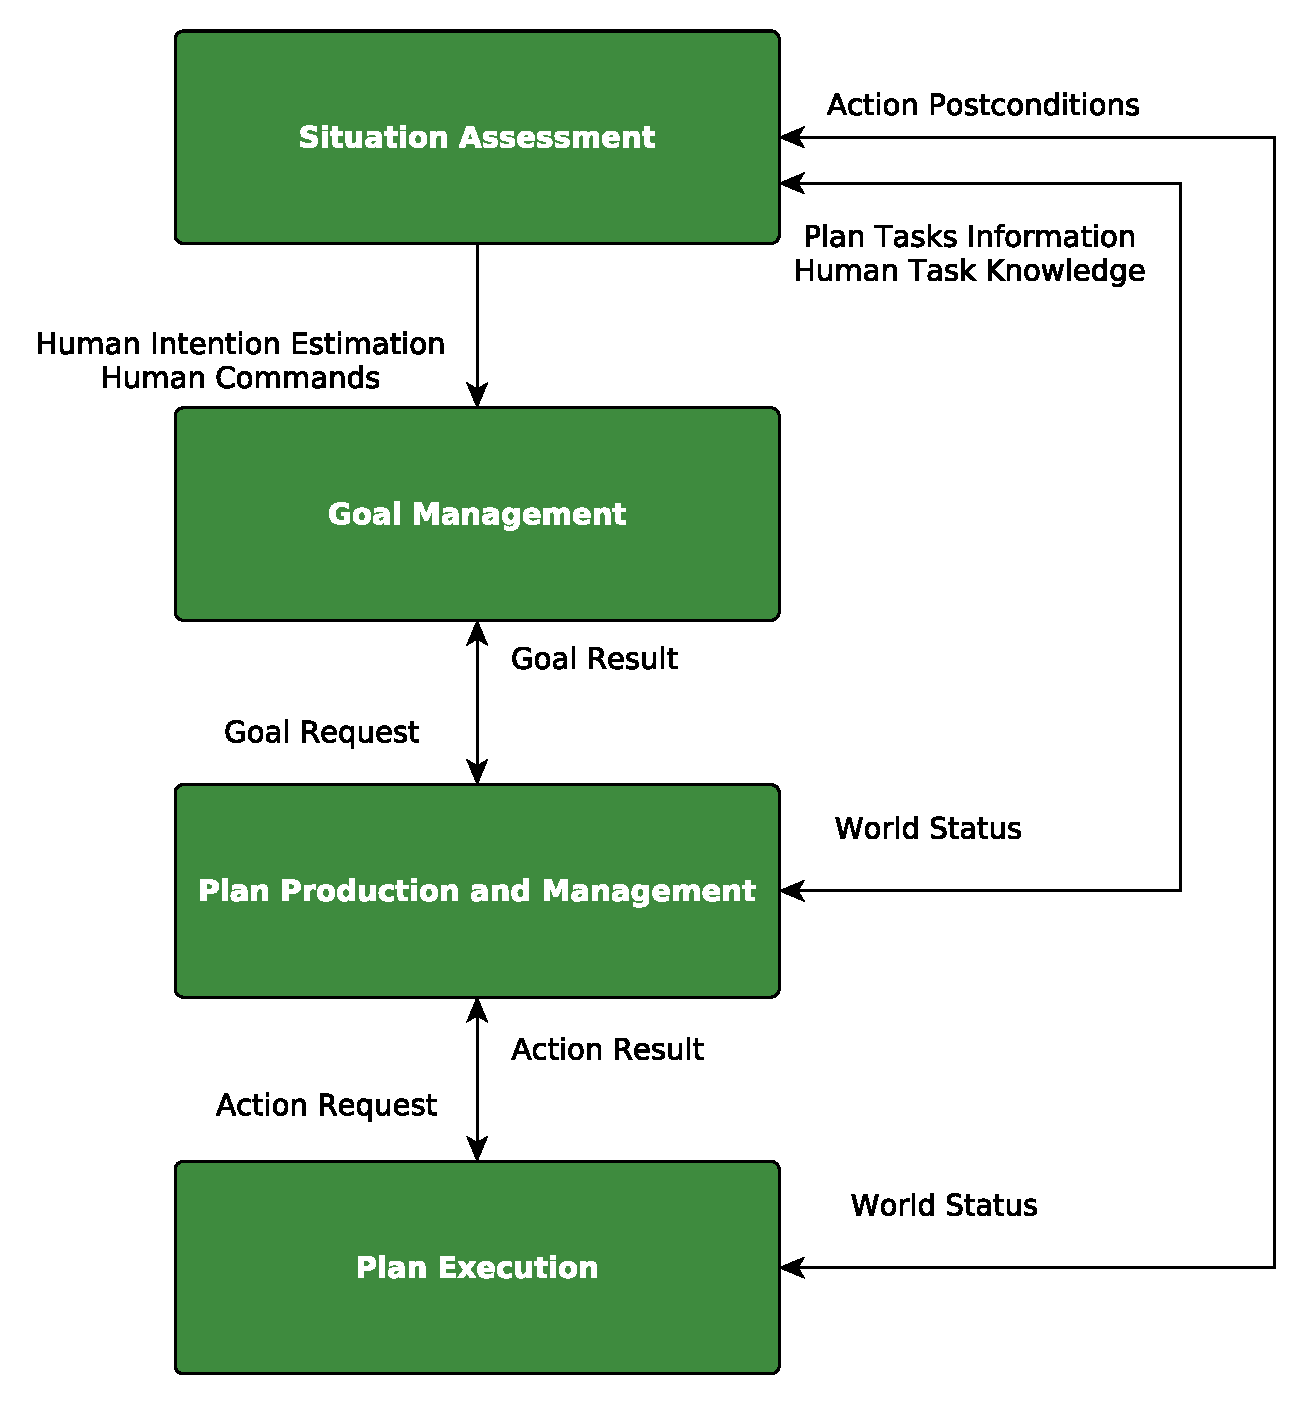
\includegraphics[scale=0.45]{img/intro/system_architecture.pdf}
	\caption[System architecture]{This picture shows the different layers of the system. Green rectangles represent parts of the
	supervision system, while blue rectangles external modules}
	\label{fig:intro-system_architecture}
\end{figure}

The system can also easily interact with different modules, which can be changed depending on the current needs:
\begin{itemize}
\item Task Planner. The Plan Management layer provides an interface for different planners. New planners can be introduced by creating a bridge that respects the interface provided, producing plans in the format requested by the Plan Management layer and reading information about the world state from the Situation Assessment layer.
\item Motion Planners and Executors. The Task Execution layer is interfaced with a set of motion planners and an executor to accomplish the robot's movements and actions. New modules can be introduced by respecting the interface used in the layer.
\end{itemize}


To achieve these goals we use the well-known ROS framework\footnote{http://www.ros.org/}, which naturally supports different robots and modules. The system has been implemented and tested in simulation, using the GAZEBO simulator\footnote{http://gazebosim.org/}, and on two different robots, the PR2 by Willow Garage\footnote{https://www.willowgarage.com/pages/pr2/overview}, and the SPENCER robot\footnote{http://www.spencer.eu/}, developed in an European research project. 

The system has been used in two european projects: SPENCER, whose tasks was building a human-aware robot to guide passengers in an airport scenario; and SAPHARI European project\footnote{http://www.saphari.eu/}, where it was used to execute a cooperative scenario, where a robot and a human had to clean a table together.

\part{The Robot Observer} % Main chapter 
\label{part:robot_observer} % Change X to a consecutive number; for referencing this chapter elsewhere, use \ref{ChapterX}

\lhead{Part II. \emph{The Robot Observer}} % Change X to a consecutive number; this is for the header on each page - perhaps a


In any application that is not entirely composed by repetitive, precomputed actions, robots need reasoning skills, which severely depend on the quality of the representation of the current environment. This representation can be more or less complex, depending on the application. 

Imagine, for example, a robot whose task is cleaning the floor of a room. In the simplest case, this robot would only be provided with an elementary set of sensors. Without the capacity to understand which areas actually need cleaning, this robot could only move through the room, randomly or with some strategy, achieving the task in a longer amount of time than what would actually be needed. 

% In a fairly simple case, this robot would rely on a map of the room and a set of lasers, or bumper sensors, to detect obstacles. 

Now, imagine a household robot that needs to actively help a family that lives in an apartment, by fetching objects, providing information, and helping to accomplish various tasks. Let us imagine that one of the members of the family, Greg, is moving in the living room, searching around, while exclaming `Where are my glasses?'. In the ideal situation, our robot would try to help Greg, by giving him information such as `They are on the table to your right', or even by fetching them for him. 

Clearly, in this scenario, the robot needs deeper reasoning skills. It needs to understand that the user is looking for its glasses, to link them to their actual physical location, to compute the spatial relationship between the table and the glasses, and to provide information in a natural way. In fact, if the robot would tell Greg that the glasses are in the position $(3.2, 5.0 , 1.3)$, Greg would likely be very perplexed. A more natural way would be to inform Greg that his glasses are on a table, whose location is pointed taking into account Greg's position.

In this case, having sophisticated sensors is, of course, important but not sufficient. The robot needs also to \textit{reason} on the sensor's data in order to produce meaningful information. For example: laser points and camera images need to be integrated to recognize objects and humans; spatial relationships  (e.g. the glasses are on the table) have to be properly modeled; actions performed by humans, and their effects on the environment, need to be recognized; and so on. 

The process of reasoning on data to produce symbolic information is called \textit{situation assessment}. Endsley explained in \cite{endsley1995toward} that this process is deeply linked to the quality of  decions of the robot.

While in many applications robots can benefit from a situation assessment component, being able to perform complex reasoning on data is particularly important in HRI. If the robot is able to take better decisions (i.e.  efficient, safe, socially acceptable, natural) than it will be perceived in a more positive manner by humans. 

Situation assessment is the fundamental skill for the \textit{robot observer}. In this part, we will show the situation assessment mechanisms of our system. Chapter~\ref{chapter:belief_management} shows how we can use geometrical reasoning in order to understand what the robot and other humans know and perceive about the current environment. Chapter~\ref{chapter:intention} shows how our robot is able to infer the current intention of a human and the actions it performs. Finally, chapter~\ref{chapter:observer_results} details a user study that we developed to validate our intention recognition algorithm.



                 % Chapter Template

\chapter{Belief Management} % Main chapter title

\label{chapter:belief_management} % Change X to a consecutive number; for referencing this chapter elsewhere, use \ref{ChapterX}

\lhead{Chapter 3. \emph{Belief Management}} % Change X to a consecutive number; this is for the header on each page - perhaps a shortened title

In this chapter we show how our system is able to manage agents beliefs. Section~\ref{sec:belief_management-intro} provides an introduction to the subject, with a discussion on some relevant works. Section~\ref{sec:belief_management-overview} shows an overview of our approach, discussing its key aspects and modules. Sections~\ref{sec:belief_management-system_inputs}  shows the simplified mechanism that we use to detect objects and humans. In section~\ref{sec:belief_management-geometrical_reasoning} we explain the geometrical reasoning capacities of our system, introducing the main symbolic facts that are computed. Finally, in section~\ref{sec:belief_management-belief_management} we show how we build human belief models starting from these facts.

\section{Introduction}
\label{sec:belief_management-intro}
%Motivation

In HRI, it is important to represent humans not as simple obstacles, but as acting entities, with different beliefs on the state of the world and with the capacity to affect the environment. 

A simple example to prove this point is related to proxemics. Normally, when we approach an object, like a table, in an empty environment, we just choose the quickest path. If, intead, the environment is populated by other people, we will follow a set of social rules, like keeping a certain distance from them. If the robot does not follow these rules, it might freighten people, for example by approaching quickly from behind the person, or be considered as `rude'.


Theory of Mind~\citep{premack1978does} is a skill used to reason about humans' beliefs and thoughts, and how they affect actions. An ability linked to this concept is perspective taking, which is widely studied in developmental literature.  Flavell in \cite{flavell1977development} describes two levels of perspective taking: 
perceptual perspective taking, the capacity to understand that other people see the world differently \citep{Tversky1999}; and conceptual perspective taking, the capacity to attribute thoughts and feelings to other people \citep{Baron1985}. 

Through perceptual perspective taking we are able to compute information such as `I can see the glasses, but you can not', `you can reach the bottle, but I can not'. Conceptual perspective taking is equally important, and allows us, for example, to understand that a friend, when choosing the flavors for its ice cream, would choose its favourites, which might differs from ours.

An important study linked to conceptual perspective taking is the \textit{divergent belief task}.  Formulated in~\cite{wimmer1983}, this kind of task requires the ability to recognize that others can have beliefs about the world that differ from the observable reality.  A typical test used to study divergent belief is the Sally and Anne test (Figure~\ref{fig:belief_management-sally_anne}). In this test, Sally and Anne are two puppets. A short scene is shown to participants, where Sally takes a ball and hides it in her basket, before leaving the room. While she is away, Anne takes the ball from Sally's basket and puts it in her  box. After Sally returns, participants are asked a question: ``Where will Sally look for her object?''. Young children, or those affected by autism, might answer (wrongly) that Sally will look for her object in Anne's box, not taking into account that she does not know that it was moved.

 \begin{figure}[ht!]
	\centering
	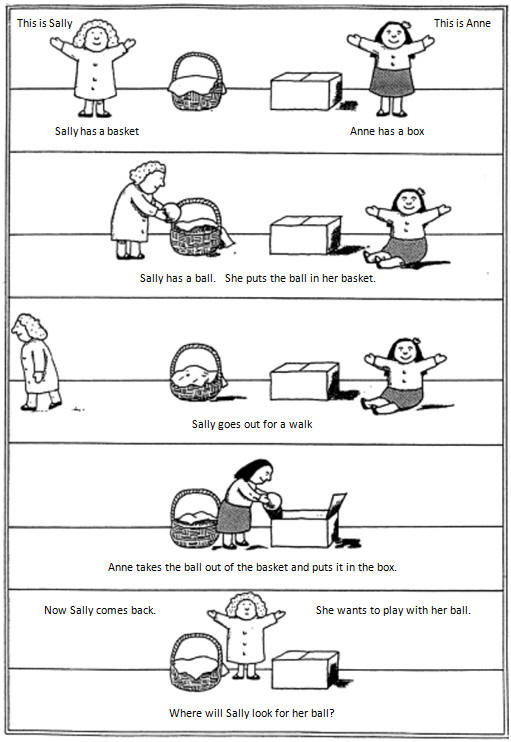
\includegraphics[scale=0.45]{img/observer/sally-anne.jpg}
	\caption{The Sally and Anne test. Original artwork by Axel Scheffler.}
	\label{fig:belief_management-sally_anne}
\end{figure}

Studies on individuals that do not possess the required mechanisms to perform perspective taking \citep{frick2014picturing} have shown that they encounter great difficulties in social relationships, confirming the importance of this ability.

These studies make us think that perspective taking could be very important in robotics. For example, let us imagine a scenario where Greg and a robot are performing some household repairs, which require the use of different tools. The robot might create a plan to achieve this goal where the human needs to use a screwdriver, which is actually behind a box, hidden from the sight of  Greg. Without perspective taking, the robot will procede in its task while Greg is desperately looking for the screwdriver. By using perspective taking, instead, the robot would infer that Greg does not know where the screwdriver is, and can not see it. In this situation, the robot might inform Greg of the location of the screwdriver, give it to him, or create a plan where Greg does not need to use it, thus being a more likable helper.

Previous works in robotics have actually demonstrated that enhancing the robot's perspective taking abilities improves its reasoning capabilities, leading to more appropriate and efficient task planning and interaction strategies \citep{Trafton2005,ros2010one,breazeal2006}. Let us review some implementations of perspective taking.

The HAMMER system, previously presented in chapter~\ref{chapter:introduction}, has been extended in~\cite{johnson2005perceptual} to introduce perceptual perspective taking, using the concept of forward and inverse visual models. Forward vision models analyze sensory data to produce information, like the geometrical coordinates of objects. Inverse visual models, instead, receive as input desired properties and states (for example, the presence of objects of a certain shape and color in a particular location), and try to produce an appropriate visual image that respects these inputs.

Perspective taking is performed by introducing two forward vision models. The first one produces the location and relationships between objects and end effectors (like grippers), while the second  computes the gaze direction of other agents. Using the results of these models as input of an inverse visual model, the system can reconstruct the scene as seen by another agent. The representation of knowledge by agents is not explicitly handled in the system. 

The architecture of~\cite{BreazealGB09}, also presented in chapter~\ref{chapter:introduction}, is another cognitive system which uses simulation mechanisms, but the work  includes both perceptual and conceptual perceptive taking. In this system the robot's schemas are used to build its mental model and execute its tasks, but also to build humans mental models and infer their actions and goals.

The robot is able to build a belief on the world state by analyzing perceptual data, producing symbolic information, such as the location or color of an object. This belief is constantly maintained, by adding new information and erasing those that are no longer valid.

To build a belief model of a human, the robot manipulates perceptual data, by filtering objects that can not be seen by the human (because they are occluded, for example), and transforming the data to simulate a first-person experience on the human. By using the same mechanisms to manage the belief for itself and for humans, the robot can infer divergent belief situations. This method has been tested on variants of the Sally and Anne test with good results.

The belief management algorithm of this systems does not take into account information that can not be directly perceived, but must be inferred. For example, in a domestic scenario, a human might not be aware that a mug containing liquid is hot and should not be touched. These aspects could be inferred by taking into account the results of actions, like pouring hot liquid in the mug.

Another system able to model agent beliefs is~\cite{scheutz2013computational}. This work is oriented toward problems where a distributed team of agents needs to communicate over a remote connection to solve a task. Each agent is assumed to be able to create its own mental model using its perception capacities, even though the precise rules for these mechanisms are not explained. When an agent receives information, he updates his mental belief using a set of rules, introducing the new data and checking for incongruencies with his previous information.  Using the same mechanism, each agent forms a belief model of other agents that have received the same information.

We created a rule-based approach for belief management, based on geometric reasoning and on inference, which we will introduce in the following sections. 

\section{Belief Management Overview}
\label{sec:belief_management-overview}

\subsection{Process overview}

Managing beliefs means being able to build and maintain a model of the belief of each agent. Our system is able to accomplish this task with different steps.

Of course, to reason on the current situation the system needs to be able to detect humans and objects in the environment. In some case, to be generic, we will call an agent or an object an \textit{entity}. Section~\ref{belief_management:entity_detection} will show how detect and track entities.

We can assign \textit{attributes} to entities, parts of entities (e.g. the arm of a human), and areas to represent different information, like properties, the state of entities or relationships between entities. Examples of attributes are:
an agent can be in a specific area; a box can be opened and can contain objects; a bottle can contain liquids; a mug can be hot; a room can be a silent area, where the robot should avoid making any noise.
We divide attributes in two classes, which influence the capacity of agents to perceive them: 
\begin{itemize}
\item Fully observable. These attributes can be observed by any present agent looking at the linked entity or area (e.g. the box is open, Greg is in the kitchen).
\item Partially observable. These attributes can be observed by present agents only in specific situations, represented as rules linked to the object and the attributes, e.g. an agent can see that a box contains items only when it is open, an agent can detect that the mug is hot only when he touches it. 
\end{itemize}

The locations of entities are integrated with other data produced by sensors through geometrical reasoning in order to produce symbolic informations, such as spatial relationships between objects and humans. We represent these information as facts. A fact is a tuple $subject\> predicate\> value$, which we use to represent symbolic knowledge. An example of fact is $CUP\> isOn\> TABLE$, which defines the location of an object. The instance of an attribute is represented as a fact, and so, each fact will correspond to exactly one attribute. More details about this aspect will be shown in section~\ref{sec:belief_management:geometrica_reasoning}.

We call \textit{world state} the collection of all facts describing the current situation. A \textit{belief model} is a collection of facts representing the knowledge of an agent on the world state. Each agent can have a different belief model, since the environment can change without an agent being able to perceive it. To represent the lack of knowledge of an agent, the value of a property can be \textit{unknown}. For example, the robot could take a tool from the table, while Greg is in another room, and place it in a box. Greg has not seen this event, and so his belief model will contain the (wrong) information that the tool is still on the table.  Section~\ref{sec:belief_management-belief_management} will show in, details, our approach to update the belief model of an agent.

In general, beliefs models are updated when the system infers that an \textit{action} has been executed, bringing a change to the environment.  We define an action as a tuple $(name, preconditions, target, postconditions)$. The $name$ of an action is a unique string that identifies it. The $preconditions$ are a set of facts that must be true in order to realize the action. In our system, an action is executed on a $target$, which can be a physical object, like a cup, but also an area of the environment, like a room. The $postconditions$ are the set of facts, and their values, affected by the action's execution.  


Since we are interested on reasoning and not perceptual aspects, we use inference, as explained in section \ref{sec:belief_management-intention_recognition}, in order to understand when a human has performed an action. Through the predefined $postconditions$ of actions we can also infer changes in the state of objects, e.g. the human opens a box, so the box is now open. 


\subsection{Architecture}
These aspects are represented in the Situation Assessment layer, and in particular in the following modules, shown in figure~\ref{fig:belief_management-belief_management_overview}.

\begin{itemize}
\item Sensor Data. Data produced by different possible sensors (e.g. lasers, camera, etc.).
\item Entity Detection. Different components detect and track humans and objects in the environment.
\item Geometrical Reasoning. Symbolic facts are produced starting from perceptual data.
\item Belief Management. The system maintains a mental model of each agent.
\item Database. The Database stores symbolic facts produced by the system.
\item Intention and Action Recognition. The system infers the current intentions of a human, and which actions are executed, by integrating  geometrical reasoning, the human's belief model, planning, and bayesian inference.
\end{itemize}

 \begin{figure}[ht!]
	\centering
	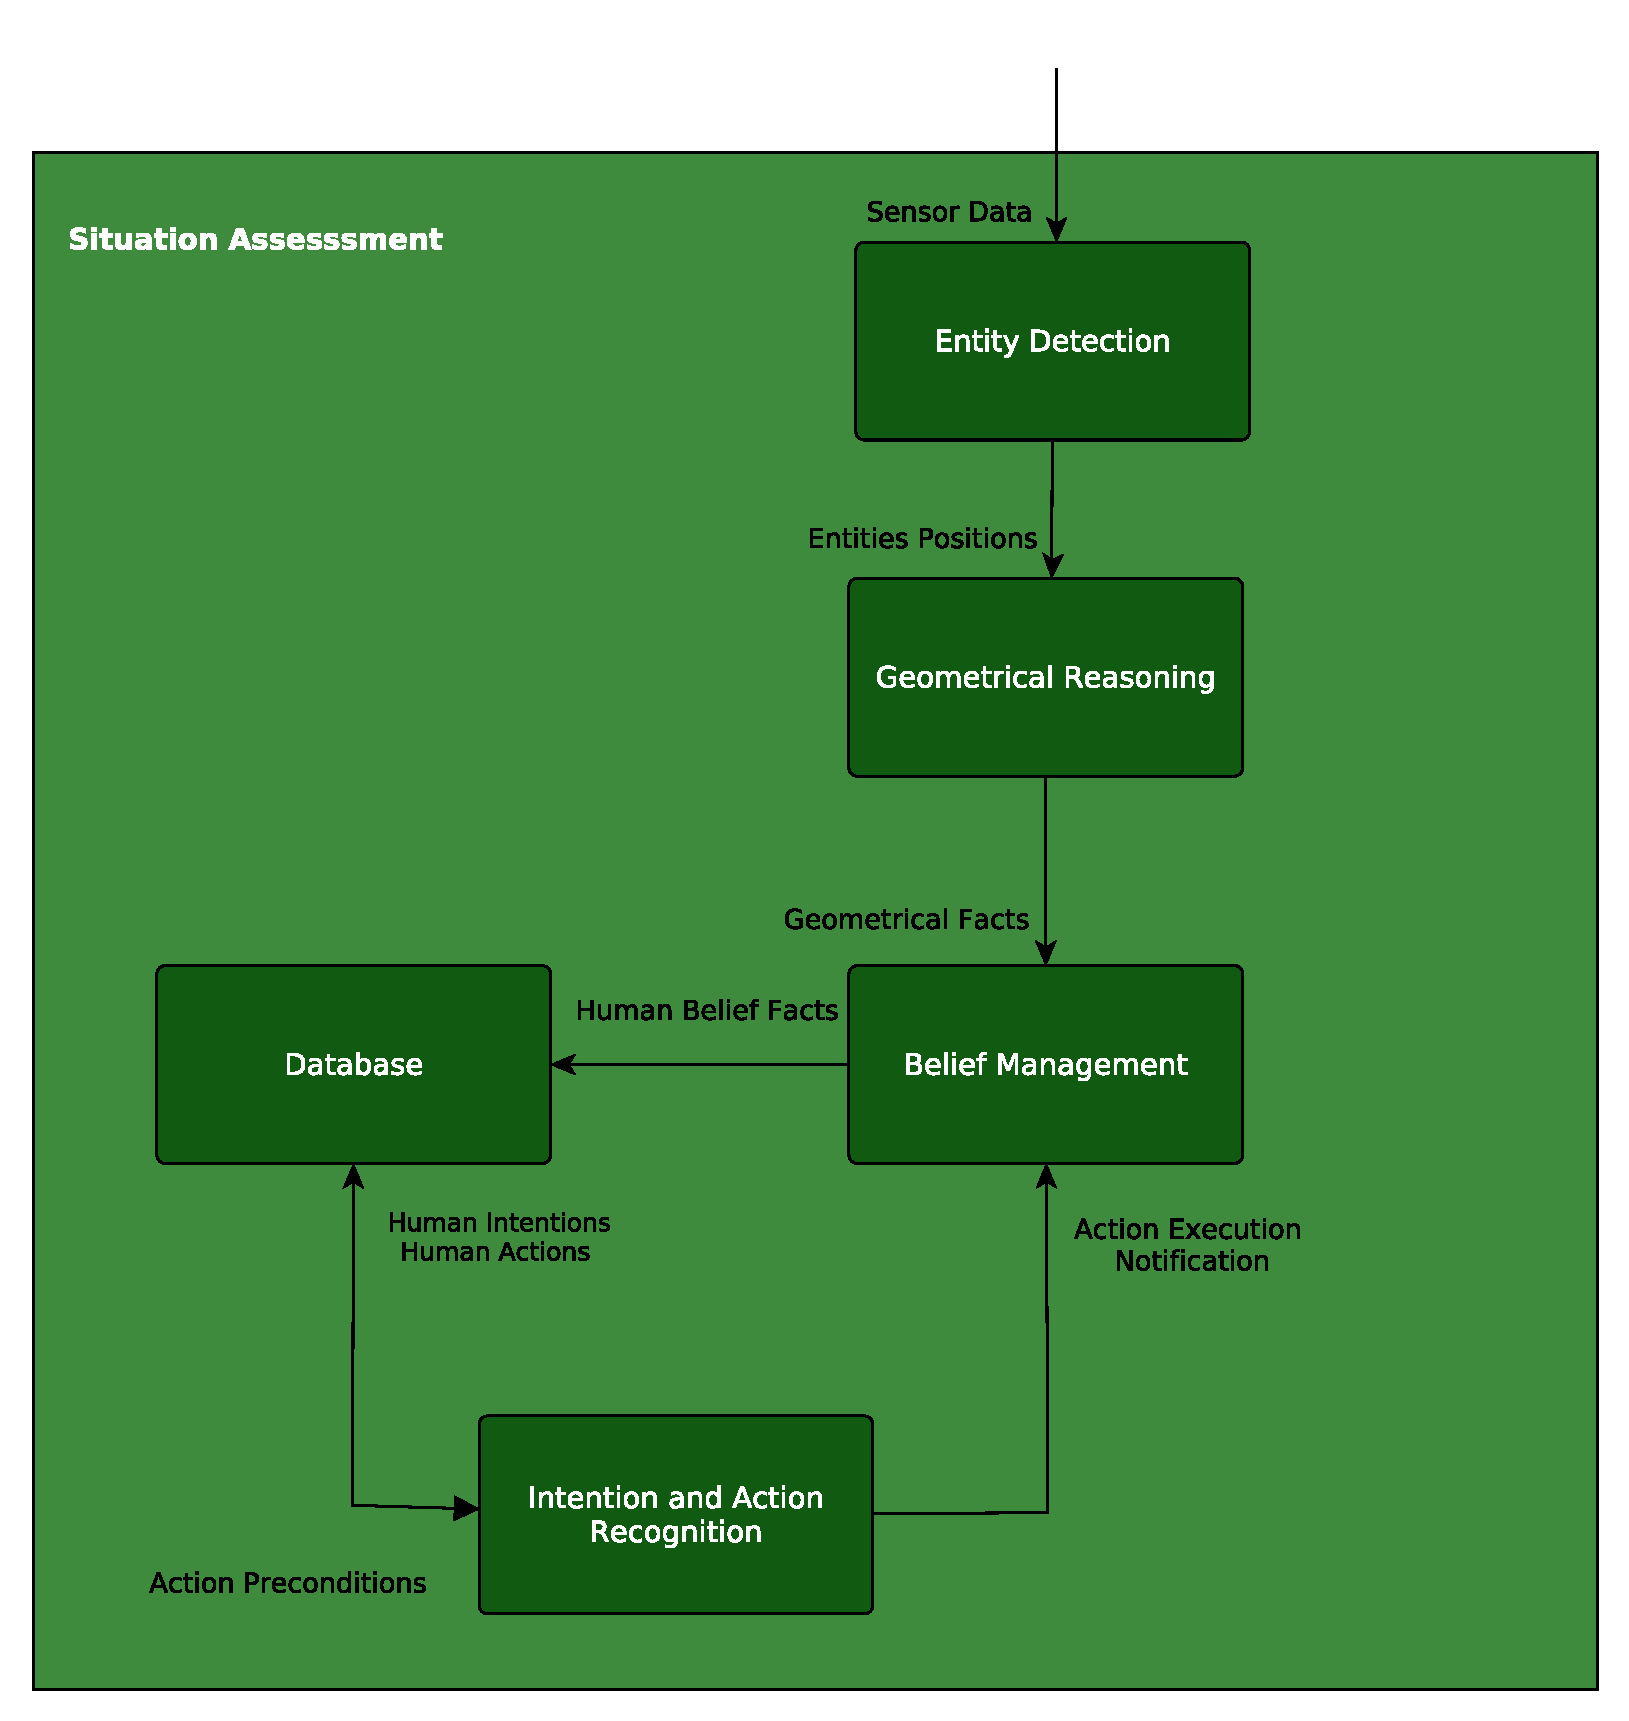
\includegraphics[scale=0.45]{img/observer/situation_assessment_overview.pdf}
	\caption{Overview of the different modules composing the Situation Assessment layer}
	\label{fig:belief_management-belief_management_overview}
\end{figure}

Symbolic facts are constantly produced, starting from the sensor data and from the position of entities. The Belief Manager collects these information to maintain the belief model of each agent. The belief model of humans and of the robot is used by the Intention and Action Recognition module to infer the most likely human intentions, and which actions they perform. All these information are introduced in the Database, and can be read by other components. For example, the Goal Management layer can choose a goal based on human commands or an estimation of humans' intentions. In a similar way, the Task Execution layer will read the Database in order to obtain the state of the world, to check action preconditions.  

The geometrical reasoning and belief management capacities of this layer were presented in \cite{Milliez2014}, where they were used to pass the Sally and Anne test~\cite{Baron1985} on a robotic platform. 

Dialogue can be a very important source of information. Agents often communicate, while executing a task together, or even when working independently, to clarify ambiguities and obtain missing information. While we will not present a specific dialogue component in this work,  in \cite{Ferreira2015} our belief management component was integrated with a situated dialogue system in a simulator. This model was compared with a basic system (without belief awareness) in a study with 60 interactions, in a simulated environment. We successfully showed that the dialogue management system significantly improves its efficiency, reducing the number of dialogue turns in the interaction, and its accuracy, with a higher success rate when a divergent belief situation appears.

In the following sections we will show how our system is able to manage agents' belief models. Actions will be treated, at this point, as input received by the Belief Management module. The intention and action recognition capacities of our system will be explained in~\ref{chapter:intention_recognition}. 

\section{Entity Detection}
\label{sec:belief_management-entity_detection}
In our system, we chose to simplify perception issues, focusing on reasoning aspects. We associate a unique tag to every object that is interesting in a particular scenario. When the robot observes a tag using a camera, it detects the corresponding object using a tag-matching algorithm.
Regarding humans, we use a motion capture software to identify and track agents moving in the environment. Using different tags, we can track the head, shoulders, and right arm of a human. Our situation assessment component has also been tested using a laser and RGB based detector, detailed in~\cite{lindermulti}, in the SPENCER european project. We also experimented using a depth camera, mounted on the ceiling, and a color-recognition algorithm to identify humans. 

 \begin{figure}[ht!]
	\centering
	\includegraphics[scale=0.7, trim={0 3cm 0 0}]{img/observer/explore.pdf}
	\caption[The robot builds a representation of the environment]{The robot explores the environment, recognizing objects through tags, and building a representation of the environment.}
	\label{fig:belief_management-explore}
\end{figure}

\section{Geometrical Reasoning}
\label{sec:belief_management-geometrical_reasoning}

Using its perception abilities the robot can build a representation of the environment, starting with entities' positions. With geometrical reasoning we can compute spatial relationships between entities, e.g. the glasses are on the shelf, the human is moving toward the library, the glasses are reachable by the human, the bottle is visible for the human. These reasonings provide a base for the perspective taking abilities of the robot.  The geometrical reasoning capacities of our system were introduced in~\cite{Sisbot2011}. This work was updated to include the production of new symbolic facts. We will show a list of some of the most important facts that our system is able to produce through geometrical reasoning.

\begin{itemize}
\item \textit{isOn}. Used when an object is on top of another, for example $CUP\; isOn\; TABLE$.
\item \textit{isNextTo}. Used when two objects are on the same surface and close to each other, for example $CUP\; isNextTo\; BOX$.
\item \textit{isReachable}. Used when an object is reachable by an agent, computed through inverse kinematics. An example of such predicate is $CUP\; isReachableBy\; ROBOT$
\item \textit{isVisible}. Used when an entity is visible by an agent. This is calculated by computing the field of view of an agent, and checking if there is a sufficient portion of the object not hidden by occlusions in this field. An example of this predicate is $CUP\; isVisibleBy\; ROBOT$.
\item \textit{isMoving}. Used when an agent is currently moving. This is computed by checking if the agent's displacements in a pre-determined time unit is bigger than a pre-determined threshold. We use an hysteresis filter to avoid continuous oscillation in the value of the fact. An example of $isMoving$ is $ROBOT\; isMoving\; TRUE$.
\item \textit{isMovingToward}. Used to indicate that an agent is moving toward a particular entity. This is computed by checking if the distance between the agent and the entity is decreasing. An example of this predicate is $ROBOT\; isMovingToward\; GREG$.
\item \textit{isOrientedToward}. Used to indicate that an agent is oriented toward a particular entity, for example $ROBOT\; isOrientedToward\; GREG$.
\item \textit{pose}. Used to indicate that an agent is in a particular pose, for example $GREG\; pose\; HANDOVER$.
\item \textit{isAt}. Used to indicate that an agent is in a particular location, for example $GREG\; isAt\; LIVING\_ROOM$.
\end{itemize}


\section{Belief Management}
\label{sec:belief_management-belief_management}
We have created a rule based framework in order to build the beliefs of each agent and update them when needed. Human belief models are updated using the perspective taking skills of the robot. When the robot detects the execution of an action in the world, with the mechanisms shown in chapter~\ref{chapter:intention_recognition},
it updates the belief model for itself and for every human that can perceive the action, adding its $postconditions$ to their models. When an action is not perceived by a human (e.g. the user was in another room), his belief model will not be updated, as he is not aware of the changes that occurred.

However, when he comes back and looks at the environment, we assign him a new belief state following a set of rules, which we will now explain. We call $p$ a fact, $H$ the agent, $HB$ his belief model, and $RB$ the robot's belief model. We also create the following predicates: $obs(p)$ means that $p$ is observable for $H$, $valid(p,x)$ means that $p$ does not contradict the current perception data of agent $x$, $value(p,m)$ is the value $p$ in belief model $m$, and $vis(p,x)$ means that agent $x$ has visibility on the linked entities of $p$ (e.g. if $p$ is $MUG\; isOn \; TABLE$ the linked entities are $MUG$ and $TABLE$) . The rules for the $valid$ predicate will be different in each attribute. For example the fact \textit{MUG isOn TABLE} will not be valid for agent Max if he can see that there is no mug on the table. For each fact $p\in HB \cup RB$:
\begin{itemize}
\item if $p \in RB, \quad p\not\in HB,\quad obs(p),\quad vis(p,H) \rightarrow value(p,HB)=value(p,RB)$.
\item if $p \not \in RB,\quad p\in HB,\quad obs(p),\quad vis(p,H) \rightarrow remove\quad $p$ \quad from \quad HB$.
\item if $p\in RB,\quad p\in HB$ then:
	\begin{itemize}
      \item if $value(p,HB)\neq value(p,RB),\\ \quad obs(p),\quad vis(p,H) \rightarrow \\ value(p,HB)=value(p,RB)$.
      \item if $value(p,HB)\neq value(p,RB),\\ \quad !obs(p),\quad !valid(p,H) \rightarrow \\ value(p,HB)=\textit{unknown}$.
	\end{itemize}
\end{itemize}
The idea of this set of rules is updating an agent's mental belief model for a fact only if it is observable, or if it is not observable and perception data contradicts the current value of the fact (e.g. the mug was moved from the table to the kitchen while the agent was in another room. While the agent can not see where is the mug, he can see it is no longer on the table).


%TODO: Image of perspective taking

 
\chapter{Inferring Human Actions and Intentions} % Main chapter title

\label{chapter:intention} % Change X to a consecutive number; for referencing this chapter elsewhere, use \ref{ChapterX}

\lhead{Chapter 3. \emph{Intention Recognition}} % Change X to a consecutive number; this is for the header on each page - perhaps a shortened title

In this chapter we show how our system is able to infer human actions and intentions. Section~\ref{sec:intention-intro} introduces the problem of intention recognition, discussing some works that studied it. Section~\ref{sec:intention-intention_recognition} shows our approach at solving this problem, while section~\ref{sec:intention-example} shows an example of a run of our algorithm.


\section{Introduction}
\label{sec:intention-intro}
A crucial skill to interact with humans is recognizing others' actions and goals. This process is is directly linked to modeling humans' beliefs, since, as explained by \cite{byom2013theory} ``as humans, we generally believe that others act in ways that are consistent with their beliefs and goals". 

The recognition of human activities is an important topic in computer science research, which can be studied at different levels. Anticipating human actions and movements allows the robot to adapt its behavior and proactively help humans, as studied in \cite{koppula2013anticipating}. 

Sequences of actions can be linked to plans, a well-known topic called plan recognition. Several approaches have been studied in this domain using, for example, classical planning \cite{ramirez2009plan}, probabilistic \cite{bui2003general} or logic techniques \cite{singla2011abductive}.

As previously said, we call an intention the wish and will to achieve a goal. Intention recognition is intrinsically linked to plan recognition, since, if an agent is acting by following a plan to achieve a goal we can assume that it has a corresponding intention. In the rest of this chapter, we will consider plan recognition as a way to recognize intentions. 

Other approaches that can be used to estimate the intention of a human are Interactive Partially Observed Markov Decision Processes (I-POMDP) and Inverse Learning. I-POMDP~\citep{gmytrasiewicz2004interactive} offer a rich framework that extends Partially Observed Markov Decision Processes (POMDP) in a multi-agent setting. Inference in these models can be extremely complex, but there have been attempts at solving this issue, like in~\cite{doshi2009monte,hoang2013interactive}. 

Inverse Reinforcement Learning~\citep{ng2000algorithms} formulates the problem of computing an unknown reward function of an agent after observing his behavior. This strategy has been applied, with Bayesian Networks (BN), in~\cite{Nagai2015}, in order to learn the mental model of another agent, and choose appropriate actions for a relationship building task. A linked approach is inverted planning, which has been applied in a bayesian framework in~\cite{baker2009action}  for human action understanding.

The use of contextual information can be used to further disambiguate complex situations. For example, if it is currently raining (context), we could think that it is more likely that Greg will look for his umbrella (intention) if he has to go out. ~\cite{Liu2014} shows a system using BNs to understand users' intentions with an emphasis on contextual information. This BN is constructed using object affordances nodes (e.g. a cup can be washed or used for drinking), context nodes (e.g. it's a hot day, the cup was recently used), and intention nodes (e.g. drinking from a cup or washing it). The causal links between contexts and intentions are learnt through a user study, which uses an online questionnaire where participants need to rate the strenght of the connection betwen an intention and a context. The work does not study how to adapt this BN to complex plans, composed by sequences of actions.

It is very important to consider humans' beliefs when estimating their intentions. In a dynamic environment, agents can execute actions, modifying the state of the world without other agents being able to perceive the changes. Let us imagine a scenario. Bob comes back home from work and would like to relax while reading. He lays down on a sofa with a book, and reaches to a nearby table to grab his glasses. He does not know that his wife, during the day, moved the glasses to another room. If we would ignore Bob's beliefs on the world (i.e. he does not know that the glasses are not on the table) we could infer that, for example, Bob would like a drink while he is sitting on the sofa, or the tv remote controller. If, instead, we would know that Bob thinks his glasses are on the table (and we would use other contextual information perhaps, like Bob's habitudes) we would be able to correctly infer Bob's current intention, that is, taking his glasses, and warn him that they are not there, perhaps even fetching them for him. 

In robotics, an interesting framework that considers this issue is the Bayesian Theory of Mind \cite{baker2014modeling}, used to represent the inference process of an observer looking at another agent's behaviors. The acting agent is modeled as a POMDP, whose richness is able to represent his possible beliefs about the world. The observer's process is modeled as a DBN, built starting from the agent's POMDP but considering his reward function (that represents his desires) as hidden. The system has been tested against some alternative models and compared, in user studies, with human capacities, to understand how well it models theory of mind. Since the models used are quite complex, scalability in the model could be an issue. Also, the study is focused on a single-agent scenario, and does not consider collaborative problems.

Let us examine the two simulation-based systems that we already presented in the previous section, HAMMER ~\cite{demiris2007prediction}, and the architecture of \cite{BreazealGB09}, and see how these cognitive architectures are able to infer actions and intentions.

The HAMMER system is organized with couples of inverse and forward models.  Inverse models receive as input the goal and state of the system, producing the motor commands which are needed to achieve the goal. Forward models, instead, receive as input motor commands and compute the predicted future state. When these two models are linked, the forward model receives as input the motor commands produced by an inverse model. This link can form a loop, with the output of a forward model returning to its inverse model, which can adjust a range of parameters if the predicted future state does not match exactly the desired state. These models can be organized in parallel schemas and used to recognize actions performed by a demonstrator. 

In this case, the demonstrator's current state, as perceived by the robot, is fed in the inverse models, which in turn sends their output to their forward models. The state predicted by the forward models are compared with the demonstrator's state at the next time step. This comparison produces a score, which can be used to infer the most likely action performed. 

Forward and inverse models can be organized in hierarchical schemas, to infer actions and plans. The complexity of these schemas could be quite significant, particularly when trying to recognize a goal which can be achieved in many different ways, depending on the context. 

\cite{BreazealGB09} uses a similar ideas, where the all the possible robot movements are represented as a graph of connected poses, with arcs representing possible transitions between the poses. This graph is used both to represent the robot's movements and to map observed trajectories. Tasks are represented as schemas, which can be organized in sequential and hierarchical structures to represent complex goals.

 When trying to infer an agent's intention the robot looks for a schema whose motor action matches the observed activities of the agent. After that, the schema is traversed in reverse in order to try to determine the real intention. The system is not able to deal with ambiguities, and this algorithm stops if it comes to a point where there is more than a possible explanation for the current behavior. 

An example of non simulation-based system in this topic can be seen in \cite{talamadupula2014coordination}. This architecture is used to coordinate human-robot teams, based on intention recognition and belief modeling. Creating and maintaining beliefs is handled using the strategy explained in ~\cite{scheutz2013computational}, presented in the previous subsection. Prediction of other humans intentions' is based on the plan recognition algorithm of \cite{ramirez2009plan}. While this algorithm uses efficient replanning to increase its efficiency, in complex domains, where the users have many different strategies to achieve a goal, the system would need to execute frequent replans to infer the actual strategy chosen by the user, which can be expensive.

Our goal was developing an algorithm able, through inference, to recognize human actions and connect them to possible intentions. To avoid errors in interpretation, we decided to use humans' belief models, and not the robot knowledge, to perform our reasonings. We also decided to use contextual information to further disambiguate our estimation. Another goal was to make this algorithm fast and scalable. 

This algorithm was introduced in~\cite{devin2016some} and we will show, in the next sections, how it was designed. 

\section{Intention and Action Inference}
\label{sec:intention-intention_recognition}
In order to infer actions and intentions, we will provide the following information to the robot: a list of known contexts, a list of known intentions, a list of known actions, a set of observations of human actions, and a belief model of humans and of the robot itself.

We introduce a simplification in our model: at each time step, a human can execute only one action and has only one intention, decreasing the ambiguities in the inference process.

We propose, as central model used for intention estimation, a framework based on BNs. We call our implementation of BN an Intention Graph (IG).
An IG is linked to a specific human, and composed by the following layers of nodes:
\begin{itemize}
\item Context Nodes: these nodes represent contextual information, modeled as boolean variables (e.g. HotDay, ColdDay).
\item Intention Nodes: these boolean nodes represent the set of possible intentions. Each intention can conditionally depend on several contexts.
\item Action Nodes. This is the set of human actions whose preconditions are satisfied when the IG is created. Each of these nodes is conditionally dependent on all the intention nodes. 
\item Observation Nodes. We associate to each action a different set of observation nodes, that depend conditionally on the associated action node. For example, the distance of a human from the \textit{target} of an action can be an Observation Node.
\end{itemize}

In a typical usage, the robot will create, for each monitored human, an IG, formed by the Context and Intention Nodes, which we consider statically known by the robot, and a variable list of Action and Observation nodes, which depends on the human's belief model. The robot will create action nodes for each known action whose $preconditions$ are \textit{satisfied in the human's belief model}, and their related Observation Nodes. We stress, in particular, that actions are created based on the human's belief model, since the human might be trying to execute actions that are actually impossible in the current situation (e.g. the human tries to take an object from a basket without looking inside it. He does not know that the object is not there anymore).  These IGs will be updated every time that an agent performs an action, creating and removing Action and Observation nodes, depending on the state of the world after the action was performed.

When monitoring a human, we set Context Nodes and Observation Nodes as \textit{evidence}, considering them observable by the robot. These information will allow us to have a good estimation of the most likely actions and intentions of the human, as explained in subsection~\ref{sec:intention-intention and action inference}. 

An example of IG, taken from an experiment, can be seen in figure~\ref{fig:intention-intention_graph}. In the following paragraphs, we will explain the role of these layers of nodes, and how the conditional dependencies between them are computed. After that, we will show an example showing how an IG is created and updated following a sequence of human actions, and how the robot is able to use it to infer the most likely human intention.

 \begin{figure}[ht!]
	\centering
	\includegraphics[trim={2cm 11cm 11cm 17cm},clip,scale=0.45]{img/observer/cookieScenario.pdf}
	\caption[Intention Graph]{A scene from our experiment. The yellow arrows show possible actions and their associated probabilities. The diagram represents the current IG. Green circles represent evidence nodes and blue circles other nodes. For the Context Nodes (top of the graph), we represented nodes with a false value as greyed out, and nodes with a true value as green. The most likely nodes in the graph are represented with a glowing effect. The observation nodes were compressed in a single block to simplify the diagram}
	\label{fig:intention-intention_graph}
\end{figure}

The following subsection will provide details on the IG, while section~\ref{sec:intention-example} will show an example of its use.

\subsection{From Contexts to Intentions}
We introduce a set of contexts in our domain. We consider as context any information that can be used to characterize and motivate an intention \citep{abowd1999towards}. We model a context  as a fact, which can assume different values and influences the probability of a user having a particular intention. For example, we imagine that a human is more likely to be cooking at dinner time, or to drink a hot mug of tea on a cold day.

Contextual nodes can directly influence one or more Intention nodes. In this work, we chose to learn these conditional dependencies from humans, as explained in section~\ref{sec:intention-experiments}.

\subsection{From Intentions to Actions}
\label{sec:intention-action_evaluation}
To understand how actions are linked to intentions the robot needs to answer the following question: what actions would a human take, in this situation, given his belief of the world, in order to achieve its intention?
Our idea is based on the principle of rationality \citep{Dennet1989}, which states that agents tend to choose the most efficient actions, taking into account their beliefs about the world, in order to achieve their desires.

In~\cite{Blakemore2001}, the authors explain that ``the attribution of intentions to actions might rely on simulating the observed action and mapping it into representations of our own intention". We represent this idea by providing the robot with a set of planning models. Each one of these planning models is related to an intention, and represents all the known plans to achieve its linked goal. In this way, we can estimate how much the current human actions are compatible with the plans related to an intention.

In our implementation, for each intention known by the robot, we will create an associated Markov Decision Process (MDP), to represent all the possible plans linked to this intention. After solving the set of MDPs we will use the calculated action value function \(Q(s,a)\), to create conditional dependencies between Intention and Action nodes in the IG. We define \(P(a|I_i=1)\), the probability that action $a$ will be performed if intention $I_i$ is true, as as:
\begin{equation}
 P(a|I_i=1)=\frac{Q_i(s,a)}{\sum_b(Q_i(s,b))}
\end{equation}
  where we normalize the value function $Q_i(s,a)$ for intention $i$ and action $a$ in the human's belief state $s$, over the value function $Q_i(s,b)$ calculated on all the monitored actions $b$. 

%   We can extend this calculation to the case where a generic number of intentions are true to compute the probabilities of action nodes: 
% \begin{equation}
%   P(a|I_1,I_2,...,I_m)=\frac{\sum_{i:I_i=1}Q_i(s,a)}{\sum_b\sum_{i:I_i=1}Q_i(s,b)}
% \end{equation}

The key idea in this problem is to use the human's belief state as input for the MDPs' value functions. In this way we are using perspective taking at a planning level, since the human action will be consistent with his intention in his own belief state but may be not optimal, irrelevant, or even dangerous in the real world (e.g. in case of wrong belief).

Our idea is similar to \cite{karami2010human}. In this work, the robot planning model is a POMDP, where the human intention is a hidden variable. The transition function for the human intention is computed starting from the action values obtained from a set of human MDPs, that simulate human policies related to different intentions. In this work, we used a BN for the inference process, instead of a POMDP. This allows us to include in a simple way more information in the inference process, such as context, and to separate the mechanisms used for inference and for the robot's actions. Also, we improve the recognition process by including the belief state of the human.

\subsection{From Actions to Observations}
Intentions will be inferred from human actions, so the robot needs to monitor their execution. For each Action Node we can define a different set of Observation Nodes, which depend on the specific actions. Typical examples are: the distance of the human's body from the action's $target$, its variation, the distance of the human's hand from the action's $target$, and its variation. The conditional dependencies of the Observation Nodes are precomputed.

\subsection{Intention and Action Inference}
\label{sec:intention-intention and action inference}
We assume, in this work, that at each moment a human can only execute a single action, and the robot will react only to his most likely intention. The most likely action and intention are inferred from the BN in the following way. We call $P(n)$ the inferred probability of a node $n$, $B(n)$ the set of brothers of $n$ (that is, nodes on the same layer), and $\delta_1$, $\delta_2$ two thresholds. The robot selects the most likely action and intention following these rules: 
\begin{itemize}
\item  \(P(n_i)>\delta_1\) 
\item  \(\forall b \in B(n_i): P(n_i)>P(b)+\delta_2\), where $n_i$ is the node associated to the interested intention or action.
\end{itemize}

To infer that an action has been performed, the robot uses an estimation of the action's probability and geometrical reasoning. For example, the robot infers that a human has taken a bottle if his hand is closer to it than a threshold $\sigma$  and the action's probability in the IG respect the previous rules. For another example, the robot infers that a human has mixed some ingredients in a bowl if his hand approaches the bowl and then leaves after some seconds, always taking into account the probability of the action in the IG.

When the robot infers that an action has been performed, it updates the world state with its $postconditions$, triggering an update on the beliefs of all present agents. The current human intention is recorded in the Database, and will be used by the Goal Management layer.

 \begin{figure}[ht!]
	\centering
	\includegraphics[scale=0.8, trim={0 4cm 0 0}]{img/observer/pick.pdf}
	\caption[Actions and world update]{The human picks an object and the robot updates accordingly the world state. The spheres surrounding objects show when the human's hand is considered to be near an object.}
	\label{fig:intention-pick}
\end{figure}

\subsection{Action Inference with Unknown Intentions}
In some situations, we are interested in inferring human actions without using information from intentions. One situation is when we the robot as a shared plan with a human. The MDPs used in our implementation are able to plan only for a single-agent, and can not be used to represent the shared plan. This could be a problem, because when agents act alone, they might execute different actions than when acting together. For example, if Greg and the robot are reordering a room together, Greg might give the robot a book, because in the shared plan the robot will put it in its place. If Greg is acting alone, he will need to place the book back by himself.  

In this situation, we will create an IG using only actions and observations. In this way, we can still infer which actions are executed, but we have to rely only on geometrical reasoning. Since we are using limited perception algorithms, we could easily encounter ambiguous situation, where, for example, the human moves his hand toward two close objects. In this situation, without using higher level information, the system could make mistakes, and infer that the wrong action has been performed.

We will discuss, in chapter~\ref{chapter:mamdp} about a possible multi-agent implementation to solve this issue.

\section{Proactive Behaviors}
\label{subsec:intention-proactive_behaviors}
Information about the most likely intention and action will be introduced in the Situation Assessment layer's Database, to be read by the Goal Management layer. Based on this information, the robot can execute two different proactive behaviors: correcting the belief state of the human, and proactively helping him to achieve his task.

\subsection{Correcting Belief State}
Having a wrong or incomplete belief on the world state can lead agents to execute non optimal, useless, or even dangerous actions. The robot needs to detect these situations in order to warn the human. For example Greg could search for his glasses in a wrong location if he does not know that they were moved, or could touch a hot object if he does not know its temperature.

 The robot assumes that it always holds a correct belief state. Our solution uses the expected action rewards introduced in \ref{sec:intention-action_evaluation}. The idea is comparing the expected reward for performing an action according to the human and the robot's belief states. To formalize: we compare the action values \(Q_m(s_h,a_h)\) and \(Q_m(s_r,a_h)\), where $m$ is the most likely intention,  $s_h$ and $s_r$ are the robot's and human's belief state, and $a_h$ is the most likely action. If these values are not equal the human expects a different outcome from its action than what should actually happen. 

We propose a simple solution, where the robot warns the human of the detected divergent belief for that action. For example, Bob wants to drink tea from a closed, opaque bottle, which the robot knows is empty (perhaps because another agent drank the last glass), while Bob does not. When he approaches the bottle, the robot detects that his most likely intention is to drink tea. 

The system calculates the expected rewards from taking the bottle in the two belief models and obtains different values. The system checks the facts related to the attributes associated to the target of the action (i.e. the bottle) in the two mental models, and extracts the differences.  Using this information, the robot corrects the divergent belief, informing the human that the bottle is now empty. 

If there is no difference in the belief models, it means that the divergent belief is actually related to a future action that the human is expected to execute. For example, let us imagine a scenario where Greg is trying to prepare a dish, requiring pasta and tomatoes. Let us imagine that Greg does not know that there are no more tomatoes, and moves to take the pasta. Using Greg's belief model, there will be a certain reward to take the pasta, since it is a necessary step to prepare the dish. In the robot's belief model, the reward will be zero (assuming that he correctly inferred the intention of Greg to prepare pasta with tomato sauce), because there are no more tomatoes. While there are is no divergent belief on attributes related to the pasta, it would be useful if the robot would inform Greg that there are no more tomatoes.

A solution is extracting an horizon of future actions from the MDP related to the \textit{prepare pasta with tomato sauce} intention. Our system can do this by simulating an update on the MDP, considering as starting state the current human belief model, choosing as actions from the agent's policy computed when solving the model, and taking as next states the most likely effects of the actions. We can repeat the reasoning on the targets of each action in this horizon, in order to find a divergent belief. 

If we can still not find a divergent belief, the robot can only inform a human that there might be a problem to achieve its goal, but it is not able to identify it.

% In our system, the Goal Management layer will detect these situations, by reading the Database, and choose a \textit{warn agent} goal (as will be explained in chapter \ref{chapter:goal_management}).

In a real scenarios, the human might have several divergent beliefs at the same time. While the robot could inform the human as soon as it detects a divergent belief, it would risk overloading him with unneeded information. For example, Greg might not know that his wife drank a mug of coffee or moved the remote control to the table, but maybe he will not need these information in the near future. We chose, with this approach, to give information about a divergent belief only when it risks impacting the actions of a human.

\subsubsection{Performing a part of the plan}
There are situations in which the robot should help the human achieve its goal by physically acting. The Goal Management layer will consider new inferred intentions as possible goals for the robot, and will communicate with the Plan Management layer to achieve them, as explained in chapters~\ref{chapter:plan_management} and~\ref{chapter:plan_execution}. 

\section{Intention Graph Example}
\label{sec:intention-example}

\subsection{Scenario}
We will now show an example of use of an IG. We start by defining a scenario with a human, Greg, and two possible intentions: drinking water and reordering a table, by moving all the objects on top of it to the kitchen. We set three different locations: a \textit{table}, a \textit{shelf}, and a \textit{kitchen}. We consider two objects: a \textit{glass} and a \textit{bottle}. Both these objects can contain water, but the \textit{bottle} is opaque and Greg can not observe if there is water or not in it. We simplify the situation by imagining that the bottle is already open. Of course, this scenario is not realistic and is chosen just to illustrate the IG. In a real situation Greg would notice that the bottle is empty when taking it, because it would be too light, or by looking through its hole.

At the start of the scenario, Greg is at the \textit{shelf}, the \textit{bottle} and \textit{glass} are on the \textit{table}, and the they are both empty.  We set a situation of divergent belief, where Greg does not know that the bottle is empty, but the robot has this information. 

We introduce two predicates: \textit{isAt}, that represented the location of an entity, and can assume the values \textit{TABLE}, \textit{SHELF}, and \textit{KITCHEN}; and \textit{capacity}, which indicates if an object contains water, and can assume the values \textit{0}, and \textit{1}. 

The belief models of Greg and of the robot are shown in table~\ref{table:intention-ig_bm}, while the set up for this scenario is shown in figure~\ref{fig:intention-ig_scenario}.

 \begin{table}[h!]
\centering
\scriptsize
\renewcommand{\arraystretch}{1.3}
\begin{tabular}{|c|c|}
\hline
Robot & Human \\ \hline \hline
GLASS isAt TABLE  & GLASS isAt TABLE \\ \hline
BOTTLE isAt TABLE & BOTTLE isAt TABLE \\ \hline
GLASS capacity 0  & GLASS capacity 0  \\ \hline
BOTTLE capacity 0 & BOTTLE capacity 1 \\ 
\hline
\end{tabular}
\caption[Belief models in the IG scenario]{Belief models for Greg and for the robot in the IG example scenario. There is a divergent belief situation, where Greg does not know that the bottle is currently empty, represented by the fact \textit{BOTTLE capacity VALUE} }
 \label{table:intention-ig_bm}    
\end{table}



 \begin{figure}[ht!]
	% \centering
	\includegraphics[scale=0.5]{img/observer/ig_scenario.pdf}
	\caption[IG Example Scenario]{The image shows the set-up for the IG example scenario. The locations are represented as different rectangles. Greg is represented as a black circle. The glass and bottle are represented, respectively, by a blue circle and a red circle.}
	\label{fig:intention-ig_scenario}
\end{figure}

We introduce two contexts in the scenario: \textit{HotDay}, representing the fact that the day is particularly warm, and \textit{AlreadyDrank}, representing the fact that the human has recently drank water.

We introduce this possible set of actions in the scenario: taking the bottle, taking the glass, filling the glass using the bottle, drinking from the glass, moving to the kitchen, moving to the table, placing the objects in different locations. We simplify this set to only include the actions relevant to this example, and so we do not include the possibilities for Greg to refill the bottle with water. Also, we consider that Greg can only hold a single object at a moment. 

\subsection{Building the Intention Graph}
We build a starting IG with the following nodes:
\begin{itemize}
	\item Context Nodes: \textit{HotDay}, \textit{AlreadyDrank}.
	\item Intention Nodes: \textit{DrinkWater}, \textit{ReorderTable}.
	\item Action Nodes: \textit{MoveTable}, \textit{MoveKitchen}. These two actions are introduced in the IG because they are the only ones whose $preconditions$ are currently satisfied, since Greg can move in any location where he is not at the moment.
	\item Observation Nodes: \textit{BodyDistanceTable}, \textit{TowardTable}, \textit{BodyDistanceKitchen}, \textit{TowardKitchen}. The \textit{BodyDistance} nodes represent the distance between Greg and an object, and can assume the values \textit{close}, \textit{medium}, \textit{far}, \textit{out of range}. The \textit{Toward} nodes are \textit{true} if the distance between \textit{Greg} and the object is decreasing, and false otherwise.
\end{itemize}


In this scenario, we precompute the probability table of the causal links between Context Nodes and Intention Nodes, and between Action Nodes and Observaton Nodes. We set a causal link between \textit{HotDay} and \textit{DrinkWater}, and one between \textit{AlreadyDrank} and \textit{ReorderTable}. In both cases, we use the following probability table:

 \begin{table}[h!]
\centering
\begin{tabular}{|c|c|c|}
\hline
Context & \multicolumn{2}{|c|}{Intention} \\ \hline \hline
& 0 & 1 \\ \hline
0  & 0.6 & 0.4 \\ \hline
1 & 0.4 & 0.6 \\ \hline
\end{tabular}
\caption[Belief models in the IG scenario]{Conditioned probabilities of the Intention Nodes in the IG example scenario.}
 \label{table:intention-ig_intention}    
\end{table}

We consider as slightly more likely that Greg wants to drink water in a Hot Day, and that he wants to reorder the table if he drank recently.

We set a causal link between each action and its observation nodes. For example, \textit{MoveTable} will have a causal link with \textit{BodyDistanceTable} and \textit{TowardTable}. In both actions, we use the following probability tables:

 \begin{table}[h!]
\centering
\begin{tabular}{|c|c|c|}
\hline
Action & \multicolumn{2}{|c|}{Toward} \\ \hline \hline
& 0 & 1 \\ \hline
0  & 0.8 & 0.2 \\ \hline
1 & 0.2 & 0.8 \\  \hline
\end{tabular}
\caption[Belief models in the IG scenario]{Conditioned probabilities of the Toward Nodes in the IG example scenario.}
 \label{table:intention-ig_toward}    
\end{table}

 \begin{table}[h!]
\centering
\begin{tabular}{|c|c|c|c|c|}
\hline
Action & \multicolumn{4}{|c|}{Distance} \\ \hline \hline
& Close & Medium & Far & Out of Range \\ \hline
0  & 0.16 & 0.2 & 0.25 & 0.39 \\ \hline
1 & 0.39 & 0.25 & 0.2 & 0.16 \\ \hline
\end{tabular}
\caption[Belief models in the IG scenario]{Conditioned probabilities of the Distance Nodes in the IG example scenario.}
 \label{table:intention-ig_distance}    
\end{table}

If Greg is executing an action, it  more likely that he is moving toward the action's $target$. For example, the \textit{MoveTable} action is more likely the closer Greg is to the table and if the distance to it is decreasing.

\subsection{Building the Human MDPs}
To set the conditioned probabilities between Intention and Action Nodes, we created two different MDPs, each related to one of the intentions. We will now show the state space $S$, action set $A$ and reward function $R$  of the two MDPs. We do not include the transition function of the model as it is extensive and does not help understanding this example.

\begin{itemize}
\item DrinkWater:
\begin{itemize}
\item $S$: $\{agent\_isAt, glass\_isAt, bottle\_isAt, bottle\_capacity, glass\_capacity\}$.
\item $A$: $\{agent\_move\_table, agent\_move\_kitchen, agent\_move\_shelf, agent\_take\_bottle, \\ 
agent\_take\_glass, 
agent\_fill\_glass\_bottle, agent\_drink\_glass, agent\_place\_bottle\_table, \\ agent\_place\_bottle\_kitchen, agent\_place\_bottle\_shelf, agent\_place\_glass\_table, \\ agent\_place\_glass\_kitchen, agent\_place\_glass\_shelf\}$.
\item $R(s,a)=1000 \quad \text{if} \\
glass\_isAt==agent\_isAt \; \text{AND} \; glass\_capacity==1  \; \text{AND} \; a==agent\_drink\_glass$.
\end{itemize}


\item ReorderTable:
\begin{itemize}
\item $S$: $\{agent\_isAt, glass\_isAt, bottle\_isAt\}$.
\item $A$: $\{agent\_move\_table, agent\_move\_kitchen, agent\_move\_shelf, agent\_take\_bottle,\\ agent\_take\_glass, 
agent\_place\_glass\_kitchen, agent\_place\_bottle\_kitchen\}$.
\item $R(s,a)=1000 \quad \text{if} \\
(glass\_isAt==kitchen \; \text{AND} \; bottle\_isAt==human \; \text{AND} \; a==human\_place\_bottle\_kitchen)  \\
 \text{OR} \\
 (glass\_isAt==human \; \text{AND} \; bottle\_isAt==kitchen \; \text{AND} \; a==human\_place\_glass\_kitchen)$.
\end{itemize}
\end{itemize}

After solving these MDPs we used their action value functions to compute the conditioned probabilities for the Action Nodes, as shown in section~\ref{sec:intention-action_evaluation}.

\subsection{Simulated Run}
We will now show a simulated run of this scenario in three steps. This run was created by introducing a stream of observations in the system, including the actions that Greg will perform. We consider that Greg's intention in this example is \textit{Drink Water}. We will conduct three different tests for each step:
\begin{itemize}
	\item Test 1. We create the IG using the human's mental belief state to compute the causal links between Action and Intention nodes. We do not use context to help disambiguate the intentions.
	\item Test 2. We add contextual information to Test 1, setting \textit{HotDay} to \textit{true} and \textit{RecentlyDrank} to \textit{false}.
	\item Test 3. We do not use contextual information and use the robot's mental belief state to compute the causal links between Action and Intention nodes. This means that the robot will evaluate Greg's action by considering that he knows that the bottle is currently empty (even though he does not know).
\end{itemize}

We will now describe and discuss these stages:
\begin{itemize}
	\item Greg is approaching the \textit{table}, as shown in figure ~\ref{fig:intention-ig_exp1}. The observations are updated correspondingly, and the probabilities of the actions are computed. The action \textit{MoveTable} has the highest probability. 
		\begin{itemize}
			\item Test 1. At this stage, the system is not able to infer the correct intention. Greg could be going to the \textit{table} to take the objects and bring them to the \textit{kitchen} or to drink water. The probability of the two intentions is both 0.50.
			\item Test 2. By using context, the system is already able to infer the correct intention. The probability of \textit{DrinkWater} becomes 0.69, and that of \textit{ReorderTable} 0.3. The robot could already fire a proactive behavior to inform Greg that the \textit{bottle} is, in fact, empty.
			\item Test 3. Without context, the system thinks that Greg is trying to reorder the table, since it is not possible to drink water because the \textit{bottle} is empty. The system would infer a wrong intention.
		\end{itemize}
	\item Greg has arrived to the \textit{table}, as shown in figure~\ref{fig:intention-ig_exp2}. The $postconditions$ of the action are added to the mental models of the robot and of Greg, changing Greg's location. The system creates a new IG, setting as actions those whose $preconditions$ are now satisfied: \textit{MoveKitchen}, \textit{MoveShelf}, \textit{TakeGlass}, and \textit{TakeBottle}. At this point, Greg's hand moves toward the \textit{bottle}, and the observations nodes are set appropriately.
		\begin{itemize}
			\item Test 1. The system is still not able to disambiguate between the two intentions. Greg could be taking the  \textit{bottle} to fill the \textit{glass} or to bring it to the \textit{kitchen}.
			\item Test 2. In this case, the context is still providing the missing information to understand that Greg wants to drink water.
			\item Test 3. In this case, since it is not possible to drink water in the robot's mental belief, the system is still inferring the wrong intention.
		\end{itemize} 
	\item Greg has taken the \textit{bottle}, and is now bringing it to the \textit{glass}, as shown in figure~\ref{fig:intention-ig_exp3}. A new IG is created, containing the actions that are now executable: \textit{MoveKitchen}, \textit{MoveShelf}, \textit{PlaceBottleTable}, and \textit{FillGlass}. In test 3, the IG created would not contain the action to fill the glass with water, since it is not executable in the robot's mental belief model, where the \textit{bottle} is empty.
		\begin{itemize}
			\item Test 1. At this point, the system has enough information to understand that Greg's intention is \textit{DrinkWater}, which assumes a probability of 0.90. The system can now fire a proactive behavior, with the robot informing Greg of the divergent belief. Even tought the action \textit{PlaceBottleTable} and \textit{FillGlass} could be ambiguous from a geometric point of view (since, in both cases, the arm of the human will approach the table), the system could infer that the action performed was \textit{FillGlass} since it is more \textit{useful} in the current situation and with the considered intentions.
			\item Test 2. Context confirms this intention, bringing the probability to 0.99.
			\item Test 3. In this case, Greg's movement would not be understood, since in the robot's mental belief model it is not possible to fill the glass with water. Greg's action would actually be inferred as \textit{PlaceBottleTable}, which has no use for any intention.
		\end{itemize}
\end{itemize}

 \begin{figure}[ht!]
	\centering
	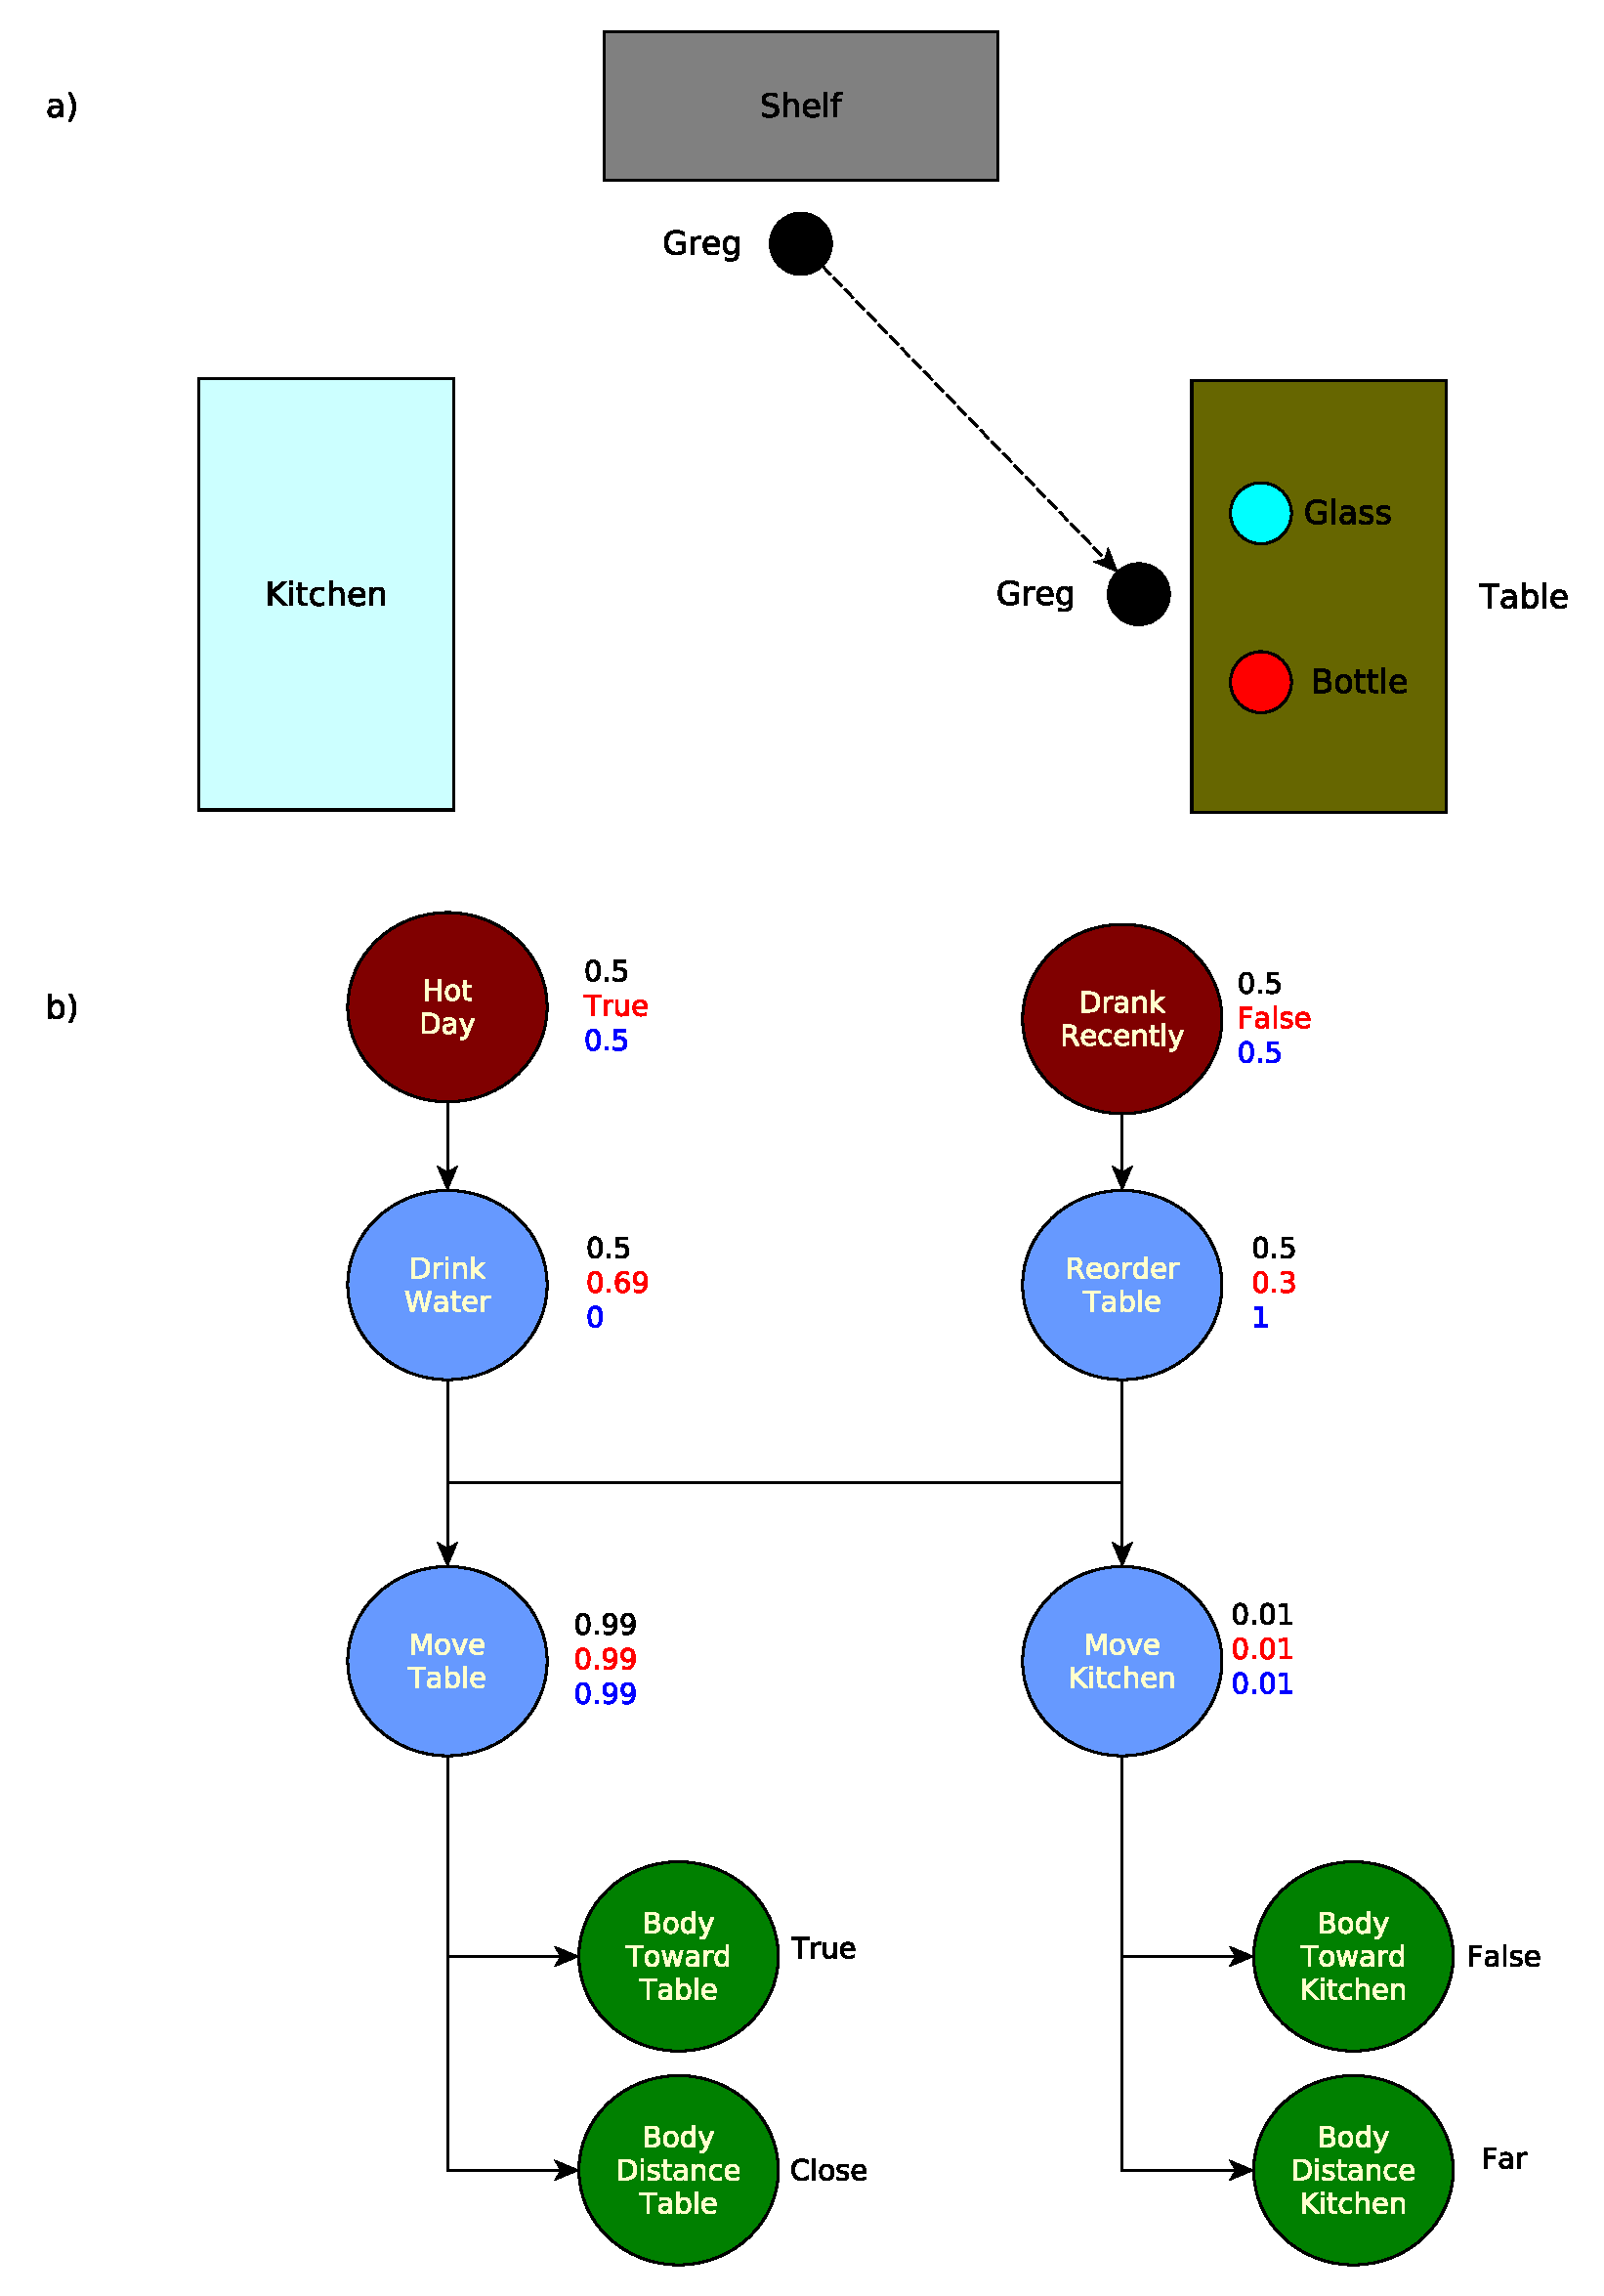
\includegraphics[scale=0.4]{img/observer/ig_exp1.pdf}
	\caption[IG Example 1]{a) Greg, represented as a black circle, is approaching the table. The two black circles correspond to his starting and ending location, with the dotted arrow showing the direction of his movement. b) The corresponding IG graph. Nodes are represented as circles and causal links as arrows. Intention and Action nodes are represented as blue. Observation nodes are represented as green to show that we consider them as evidence, fixing their values. Context nodes are represented in yellow to mean that in the first and third test they are treated as standard nodes, and in the second as evidence.
 	 For each node we show the probability that its value is true or its current value, if it is treated as evidence. We show three different values for each node: the black one shows the value if we compute the probability by using the human's mental belief (test 1), the red if we use the human's mental belief and treat context nodes as evidence (test 2), and the blue if we do not use context and use the robot's mental belief for the computation (test 3). Test 1 shows that at this point the system is not able to disambiguate between the two intention, which have a value of 0.50. Test 2 shows that context would help the robot to infer correctly the intention. Test 3 shows that by not using the human's mental belief the robot would discard the drink water intention, considering it not achievable.}
	\label{fig:intention-ig_exp1}
\end{figure}

\clearpage

\hfill
 \begin{figure}[ht!]
	\centering
	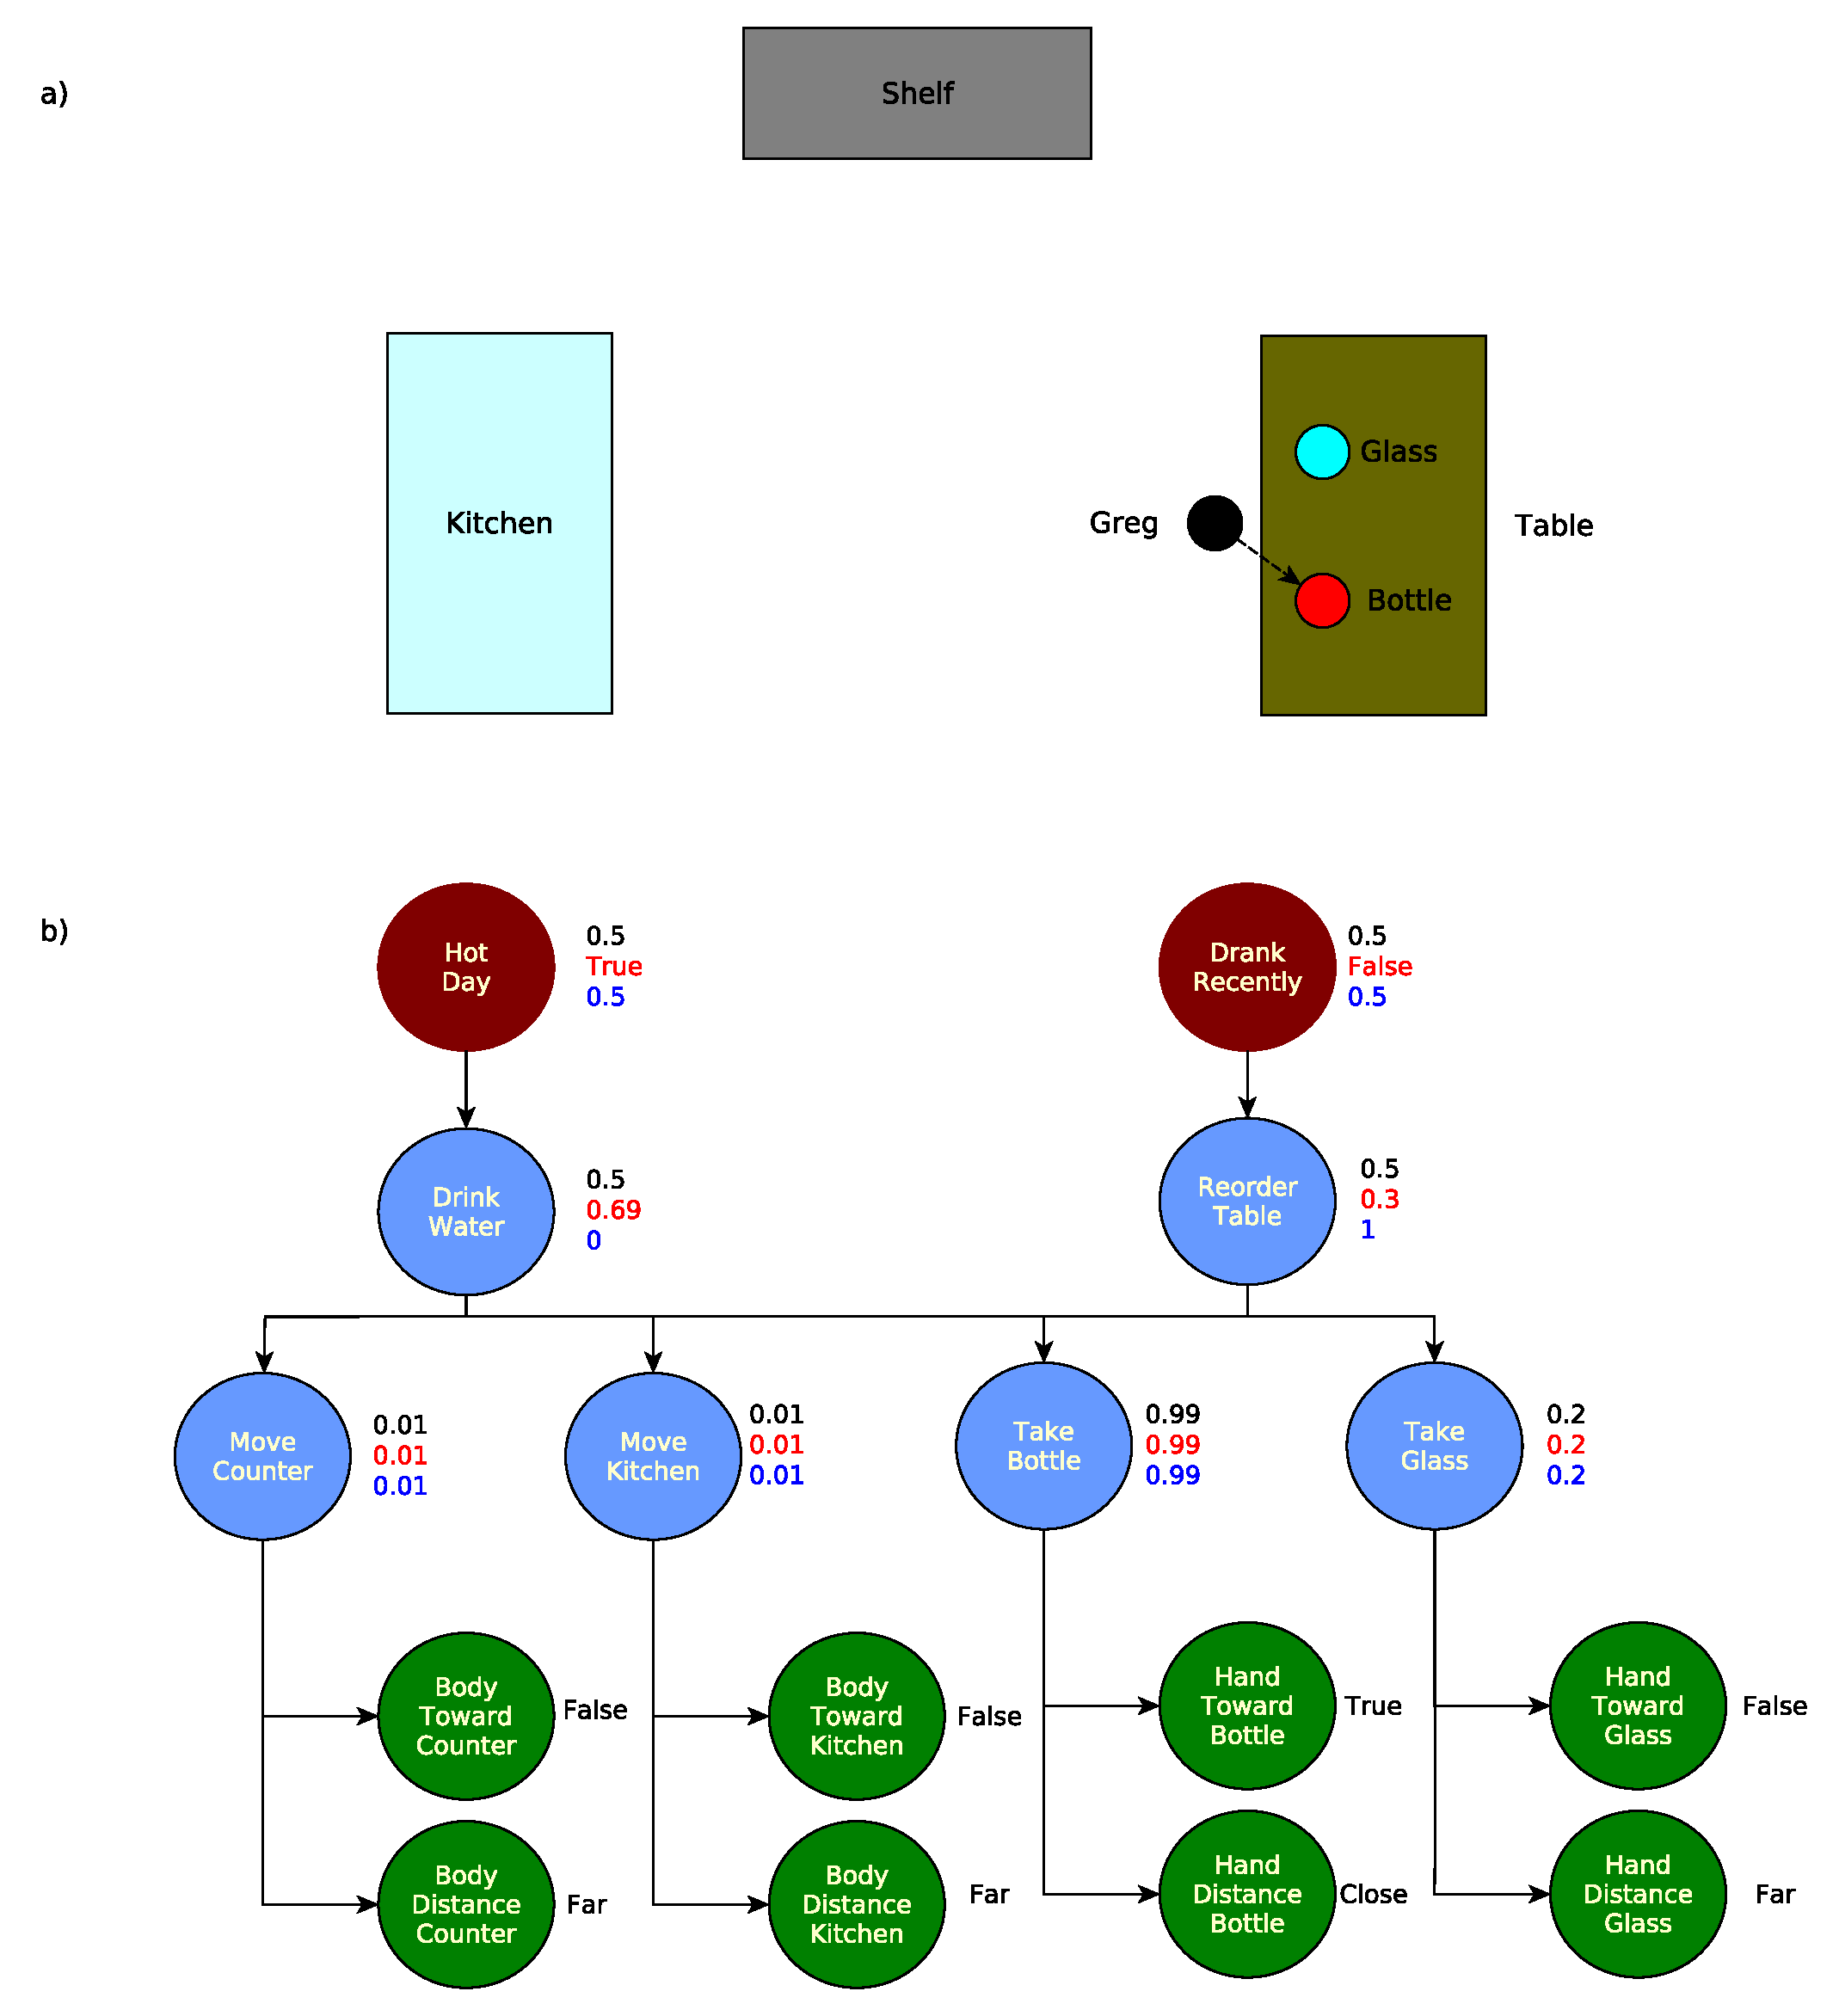
\includegraphics[scale=0.4]{img/observer/ig_exp2.pdf}
	\caption[IG Example 2]{a) Greg's hand is approaching the bottle. b) The corresponding IG graph. As before, test 1 is shown in black, test 2 in red, and test 3 in blue. The results of 
	the test are very similar to the previous time step, shown in figure~\ref{fig:intention-ig_exp1}.}
	\label{fig:intention-ig_exp2}
\end{figure}

\clearpage
 \begin{figure}[ht!]
	\centering
	\includegraphics[scale=0.4]{img/observer/ig_exp3.pdf}
	\caption[IG Example 3]{a) Greg has taken the bottle, shown by placing the red circle and black circle close. His hand, with the bottle, is now approaching the glass b) The corresponding IG graph. As before, test 1 is shown in black and test 2 in red. Test 3 is not shown since the fill glass action would not be executable in the robot's mental belief model, and so the corresponding IG would be different. In test 1 the system has now sufficient information to infer the corrent intention, which has a value of 0.98. Test 2 confirms this choice.}
	\label{fig:intention-ig_exp3}
\end{figure}
\clearpage

\section{Discussion}

This component is able to estimate the likelihood of a human's intention by combining BNs, MDPs, geometrical reasoning, and the capacity to model human's beliefs. Contextual information can further help to disambiguate the inference process. 

Another advantage of our approach is its good scalability. Computing the probabilities in a BN can be done using efficient and well know algorithms, which scale well with the size of the network, meaning that the IG is able to accomodate the addition of new actions, observations and contexts. 

Adding a new intention means creating and solving another MDP. Since this process is done offline this would not impact the run of the system. When computing the conditional probabilities of the action nodes, the system uses the action value function of the MDPs, which is stored in memory and can be directly accessed.
 
\chapter{Results and Experiments} % Main chapter title

\label{chapter:observer_results} % Change X to a consecutive number; for referencing this chapter elsewhere, use \ref{ChapterX}

\lhead{Chapter 4. \emph{Results and Experiments}} % Change X to a consecutive number; this is for the header on each page - perhaps a shortened title

This chapter presents an experiment used to evaluate the intention recognition capacity of our system. Section~\ref{sec:observer_experiment-case_study} introduces our case study, where we decided to compare the prediction of our system with those of humans. Section~\ref{sec:observer_experiment-experiment} explains how the experiment was actually conducted. We show and discuss our results in section~\ref{sec:observer_experiment-discussion}.


\section{Case Study}
\label{sec:observer_experiment-case_study}
\subsection{Study Description}

Evaluating the capacity of the system to estimate human intentions is not easy, since intentions are not directly observable. A possible solution, as shown in~\cite{baker2014modeling}, is comparing the estimation of human intentions, performed by other humans, with the predictions of our system. In order to perform this comparison we created a user study where we showed participants several videos, asking them to estimate the likelihood of a set of intentions  for each video, and collected their results. The same tests were simulated on the system, streaming as input a sequence of observations  corresponding to the actions shown in the video (e.g. if the video shows a human approaching the table, we will stream to the system a trajectory of coordinates that leads to the table position). All of the test videos ended in a situation of ambiguity. For example, in one test we showed a human approaching a table with different objects, and stopped the video before users could see which object the human wanted to take. Some videos include more information than others, like comments by humans or situations that help to disambiguate the intention. 

We have performed an equivalence test, comparing users' intentions predictions with those of the system, following the two one-sided tests (TOST) approach. We choose as a threshold for equivalence the standard deviation $\sigma$ of the users' answers. The idea behind this choice is that, if the system's answers are closer than a standard deviation to the average human answers, its predictions are comparable to an average human answer from our user group. 

We defined our hypothesis as follow: 
\begin{itemize}
\item $H_0$: $\mu_{hi}-\mu_{si}\leq-\sigma_{hi}$ \; \text{OR} \; $\mu_{hi}-\mu_{si}\geq\sigma_{hi}$ 
\item $H_A$: $-\sigma_{hi}<\mu_{hi}-\mu_{si}<\sigma_{hi}$  
\end{itemize}
where $\mu_{hi}$ and $\mu_{si}$ are the human average and the system's answer for test $i$, $\sigma_{hi}$ is the variance of the human answers for test $i$.

We have performed tests to evaluate: a) prediction in absence of clues, b) prediction in the presence of contextual clues, c) prediction in the presence of belief state clues.

We have built a household environment with a fixed set of furniture: a \textit{Kitchen Shelf}, a \textit{Table}, a \textit{Sofa}, and a \textit{Chair}. In this environment, we have created two scenarios, composed by several tests, with two agents, \textit{Max} and \textit{Bob}, performing different actions. Each scenario contained a set of objects, and a constrained set of intentions. For the tests related to belief states, we start by showing the users a specific sequence of events, allowing them to build a mental model of the agents. A corresponding simulated sequence will be streamed to the system for this test.
We will describe in details the two scenarios and the relative tests.

\subsection{Cookie Scenario}
\begin{itemize}
\item Objects: a \textit{Cookie Box}, a \textit{Mug}, and a \textit{Bottle of Water} were placed on the \textit{Table}, close to each other. A pack of \textit{Cookies} was placed on the \textit{Kitchen Shelf}. The \textit{Cookie Box} could contain, or not, \textit{Cookies}.
\item Intentions: \textit{Eating a Cookie}, \textit{Drinking Water}, \textit{Reading the Book}.
\item Tests:
\begin{itemize}
	\item \textit{No Clues}: \textit{Max} approaches the \textit{Table}.
    \item \textit{Contextual Clues}: \textit{Max} approaches the \textit{Table} commenting on the warmth of the day.
	\item \textit{Divergent Belief No Cookies}: \textit{Max} approaches the \textit{Table}.
	\item \textit{Divergent Belief Cookies}: \textit{Bob} approaches the \textit{Table}.
\end{itemize}
\item  \textit{Divergent Belief Event}:  \textit{Max} and \textit{Bob} are chatting on the \textit{Sofa}. Max eats the last \textit{Cookie} from the \textit{Cookie Box} before closing it and leaving. While \textit{Max} is away, \textit{Bob} takes \textit{Cookies} from the \textit{Kitchen Shelf}, fills the \textit{Cookie Box} with them, and closes it, before leaving.
\end{itemize}

The \textit{Divergent Belief Event} was shown to the users (and its simulation streamed to the system) between the \textit{Contextual Clues} and the \textit{Divergent Belief No Cookiies} events. 


We have deliberately included an intention, \textit{Reading the Book}, without placing a book in the visible environment, introducing a confusing element in the scenario. This scenario can be seen in figure~\ref{fig:observer_experiments-cookie}.


 \begin{figure}[ht!]
	\centering
	\includegraphics[scale=0.5]{img/observer/cookie1-blur.pdf}
	\caption{The cookie intention scenario}
	\label{fig:observer_experiments-cookie}
\end{figure}


\subsection{Keys Scenario}
\begin{itemize}
\item Objects: a \textit{Box} was placed on the \textit{Table}, that partially occluded the sight of people approaching. A \textit{Book} and a \textit{Mug} where placed behind the \textit{Box}, so that they could be seen from the sofa but not from approaching people.
\item Intentions: \textit{Taking the Mug}, \textit{Taking the Keys}, \textit{Reading the Book}.
\item Tests and Events:
\begin{itemize}
\item \textit{No Clues}: \textit{Max} approaches the \textit{Table}.
\item\textit{Contextual Clues}: \textit{Max} approaches the \textit{Table} in a hurry, while putting on a coat.
\item \textit{Divergent Belief Max}: \textit{Max} approaches the \textit{Table} in a hurry, while putting on a coat.
\end{itemize}
\item \textit{Divergent Belief Event}: \textit{Max} is sitting on the \textit{Table}, drinking from the \textit{Mug}, while having the \textit{Keys} in his hands. His phone rings, so he drops the \textit{Keys} and the \textit{Mug} on the \textit{Table}, behind the \textit{Box}, and leaves the room. While \textit{Max} is away, \textit{Bob} comes and sits on the \textit{Sofa}, reading a \textit{Book}. When he sees the \textit{Keys}, he takes them, places the \textit{Book} on the \textit{Table}, and leaves.
\end{itemize}

The \textit{Divergent Belief Event} was shown to the users (and its simulation streamed to the system) between \textit{Contextual Clues} and the \textit{Divegent Belief Max} events. This scenario can be seen in figure~\ref{fig:observer_experiments-keys}.

 \begin{figure}[ht!]
	\centering
	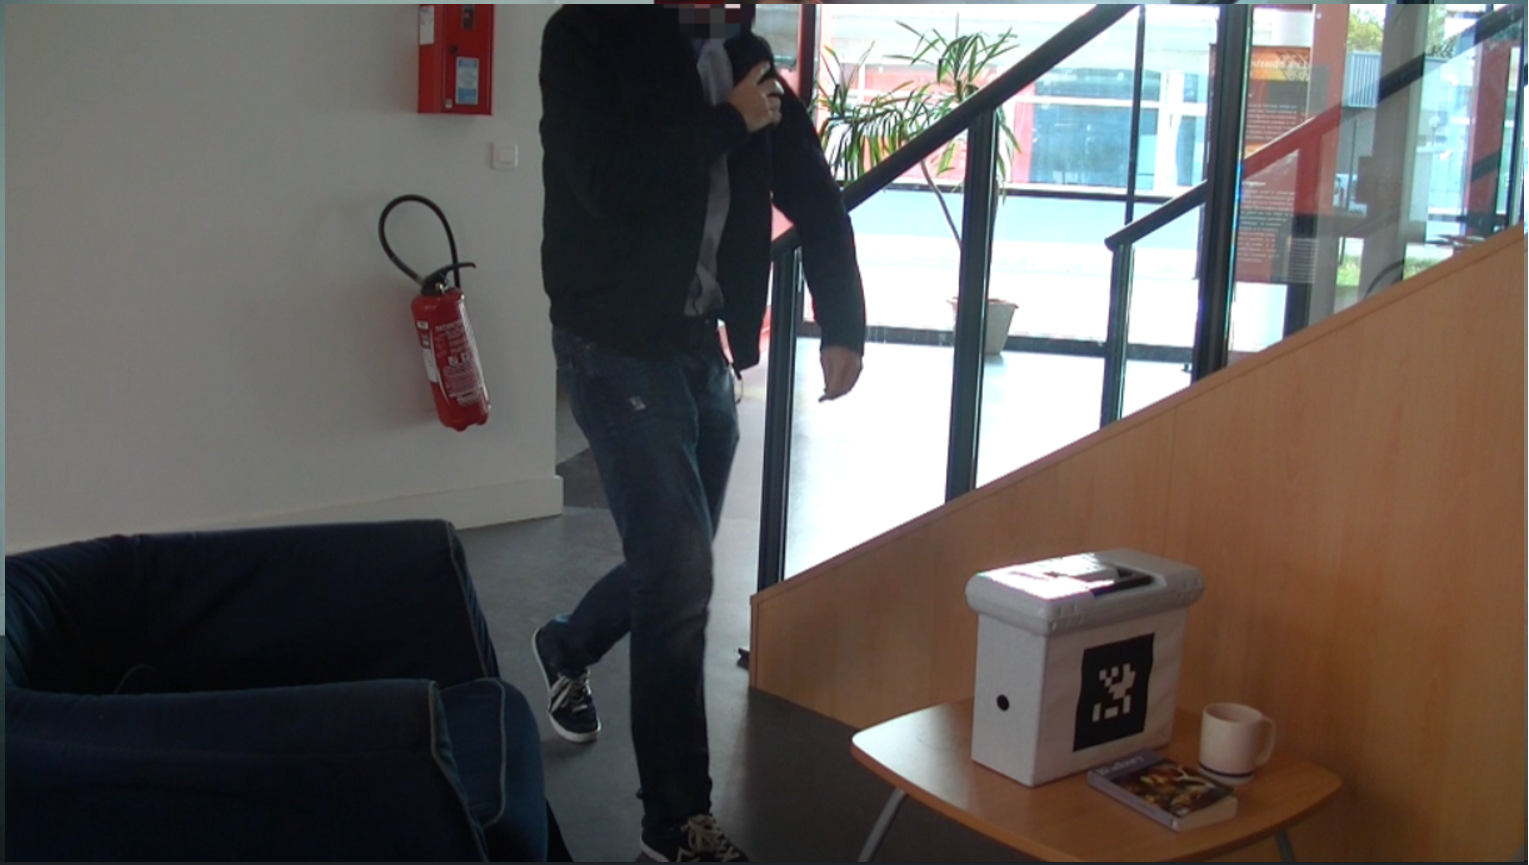
\includegraphics[scale=0.5]{img/observer/keys2-blur.pdf}
	\caption{The keys intention scenario}
	\label{fig:observer_experiments-keys}
\end{figure}

\section{Experiment}
\label{sec:observer_experiment-experiment}
\subsection{User Study}
We built an online user study, where we presented videos related to the tests and events of the two scenarios to users, who had to evaluate the likelihood of each intention of the scenario
on a five-level Likert scale. The user study was conducted in three languages, with users living in two different countries\footnote{A version of this user study was provided at http://goo.gl/forms/YiuFHnF63c}. We collected answers from 78 adults, performed an average, and converted them to percentile scores, in order to compare them with the system's predictions.

Looking at users' answers (figure \ref{fig:observer_experiments-user_study_results}), we can see that, in the absence of clues, people rated similarly the two intentions related to visible objects. Contextual clues had the highest influence on users' ratings. This is particularly visible in the \textit{Contextual Clues} test of the \textit{Keys Scenario}, where users chose as the most likely intention \textit{Take Keys}, even if no keys were visible in the video. Divergent beliefs also influenced users decisions, but not as strongly as context. The strongest responses, over all, where given by the \textit{Divergent Belief Max} test on \textit{Keys Scenario}, which uses both divergent belief and contextual information.

\subsection{System Implementation}
\label{subsec:observer_results-system_implementation}
In this subsection, we show how we implemented this experiment on our system. We will start by showing how we created a simulation of the scenarios. Then we will explain how we computed conditional dependencies between intentions and contexts, and finally we will discuss about the actual implementation of the IGs in the two scenarios.

\subsubsection{Setting up the Simulation}
% At the start of a scenario the robot scanned the environment, building a model of its world state. 
We built a simulation to represent these two scenarios. For each scenario, we set the positions of the objects and computed a starting world state.

 At the start of the scenario, the system does not have information about what each human knows, and so it will assume that they have the same belief model as itself. The system will be able to form a different belief model of each human only with the \textit{Divergent Belief} event. This is a simplification. In the real world, we believe that humans have complex mechanisms to infer others' mental beliefs, based on many aspects. For example, if we would go to the home of a friend, we would probably infer that he has knowledge even about attributes that he can not immediately perceive (e.g. he will know that that he can find a glass in a cabinet in the kitchen even if he can not see it at the moment). Instead, if other people come at our home, we would infer that they do not know where objects are located until they see them. Our system is not able to replicate this idea, leading to our simplification.

 For each test of our simulation, we streamed coordinates related to the body and hand positions of agents, following what was shown in the videos of the user study. For example, if in a test we showed Max moving from the hallway to the table, we streamed a trajectory of coordinates representing this path. 

The inference process was performed by building different IGs for the scenarios. Each test had a different graph, related to its main agent. 

\subsubsection{Contextual Information}
We considered three different Context Nodes for our simulation: \textit{Hot Day}, true when the day is particularly warm; \textit{Break Time}, true when the agents are taking a pause; \textit{Time to Leave}, true when it is late in the day, and the humans usually leave work and return home.

As previously said, we have chosen to follow \cite{Liu2014} in order to learn the link between Context and Intention Nodes. We submitted a questionnaire to 15 users with 16 questions, representing every possible combination of the intentions and contexts used in our scenarios. In each question,
the users had to rate how they perceived that a context influenced a particular intention. The rating was based on a five-level Likert scale, representing the range (\textit{very negatively}, \textit{very positively}). For example, one of the questions asked how a very warm day would influence the probability that the user would drink water.

The conditional dependency between intention $I_i$ and context $C_j$ was computed in the following way: 
\begin{equation}
 P(I_i|C_j=1)=\frac{\sum_{k=1}^5 ncj_k \times v_k}{n\_users}
\end{equation}

where $ncj_k$ is the number of persons who rated the influence of context $C_j$ on intention $I_i$ with the value $k$, $v_k$ is the probability value that we associated to $k$ (where 1=0.1, 2=0.3, 3=0.5, 4=0.7, 5=0.9) and $n\_users=15$ is the number of users that participated in the test.

We set the values of Context Nodes manually in the tests, depending  on the information shown in the videos. While we simulated this aspect, we will give some ideas on how the values of these Context Nodes could be inferred in a real scenario.

\begin{itemize}
\item \textit{Hot Day}. The temperature of the day could be measured by a sensor or obtained from a meteo application. Also, in one of the tests Max is commenting that the day is very warm. A speech recognition software could capture this information.
\item \textit{Break Time} and \textit{Time to Leave}. These information could be either hardcoded (e.g. in the company, workers have an hour of break from 13 to 14 and leave at 17:30) or learnt by observing the agents' activities.
\end{itemize}



\subsubsection{Cookie Scenario}
The starting world state for the cookie scenario is shown in table~\ref{table:observer_results-system_starting_state_cookie}.

 \begin{table}[h!]
\centering
\scriptsize
\renewcommand{\arraystretch}{1.3}
\begin{tabular}{|c|c|}
\hline
MUG isAt TABLE    \\ \hline
BOTTLE isAt TABLE  \\ \hline
COOKIEBOX isAt TABLE   \\ \hline
COOKIEBOX capacity 1    \\ \hline
COOKIES\_SUPPLY isAt KITCHEN    \\ \hline
\end{tabular}
\caption[Starting World State for the Cookie Scenario]{The starting world state for the cookie scenario.}
 \label{table:observer_results-system_starting_state_cookie}    
\end{table}


 With our perception capacities, we would not be able to detect if the cookie box is full or empty, and so we consider it as full (using the attribute $capacity$, which can have a value of 1 or 0) at the start of a test, and update its value using the $postconditions$ of inferred human actions. We consider the box as empty when we infer that a human has taken a cookie from inside, and as full when we infer that a human has put a cookie in it.


In the \textit{Cookie Scenario} the graph for the tests is constructed from the following nodes:
\begin{itemize}
\item Context Nodes: \textit{Hot Day}, \textit{Break Time}, \textit{Time to Leave}
\item Intention Nodes: \textit{Fill Cookie Box}, \textit{Eat Cookie}, \textit{Drink Water}, \textit{Read Book}.
\item Action Nodes: \textit{Move to Table}, \textit{Move to Kitchen}.
\item Observation Nodes: distance of the agent's body and hand to each action's associated \textit{target}.
\end{itemize}

We introduce the \textit{Fill Cookie Box} intention, not present in the human test, to allow the system to detect when Bob fills the \textit{Cookie Box} during the \textit{Divergent Belief Event}.

As previously said, we set Context Nodes to plausible values, that could be extracted by watching the videos. For the \textit{Contextual Clues} test, we set the value of \textit{Hot Day} to true (since Max is commenting about the temperature), and \textit{Break Time} and \textit{Time to Leave} to false (since no data in the video points to one of these contexts being true. Max and Bob seem to have taken a break from work before the other events are shown, in the Divergent Belief Event).

\textit{Divergent Belief Event}, \textit{Divergent Belief No Cookie}, and \textit{Divergent Belief Cookie} were streamed sequentially to the system, which updated the agents' mental models and created new IGs accordingly.
After the \textit{Divergent Belief Event}, the robot inferred that Max has a divergent belief on the \textit{Cookie Box}, because he does not know that Bob filled it. The mental states of the two humans, at this point, is shown in table~\ref{table:observer_results-divergent_event}.


\begin{table}[h!]
\centering
\scriptsize
\renewcommand{\arraystretch}{1.3}
\begin{tabular}{|c|c|}
\hline
Bob & Max \\ \hline \hline
MUG isAt TABLE   & MUG isAt TABLE \\ \hline
BOTTLE isAt TABLE  & BOTTLE isAt TABLE \\ \hline
COOKIEBOX isAt TABLE   & COOKIEBOX isAt TABLE \\ \hline
COOKIEBOX capacity 1  & COOKIEBOX capacity 0   \\ \hline
COOKIES\_SUPPLY isAt KITCHEN & COOKIEBOX\_SUPPLY isAt KITCHEN  \\ \hline
\end{tabular}
\caption[Belief models of Max And Bob after the Divergent Belief Event]{The table shows the belief models of Max and Bob after the Divergent Belief Event. } 
 \label{table:observer_results-divergent_event}    
\end{table}



 During the \textit{Divergent Belief Event} several IGs need to be created with different Action and Observation Nodes, to follow the sequence of actions by the two agents. For example, when \textit{Max} leaves the room, \textit{Bob} has the possibility to execute the actions \textit{Take Mug}, \textit{Take Water Bottle}, \textit{Open Cookie Box}, \textit{Move to Kitchen Shelf} or \textit{Leave Room}. Intention and Context nodes remains the same in all the IGs of the scenario.



\subsubsection{Keys Scenario}
The starting world state for the keys scenario is shown in table~\ref{table:observer_results-system_starting_state_keys}.

 \begin{table}[h!]
\centering
\scriptsize
\renewcommand{\arraystretch}{1.3}
\begin{tabular}{|c|c|}
\hline
BOX isAt TABLE    \\ \hline
BOOK isAt TABLE  \\ \hline
MUG isAt TABLE   \\ \hline
\end{tabular}
\caption[Starting World State for the Keys Scenario]{The starting world state for the keys scenario.}
 \label{table:observer_results-system_starting_state_keys}    
\end{table}

The IG for this scenario is similar to the one for the \textit{Cookie Scenario}, with the following differences.
\begin{itemize}
\item Context Nodes: \textit{Hot Day}, \textit{Break Time} and \textit{Time to Leave}.
\item Intention Nodes: \textit{Drink Water}, \textit{Take Keys}, \textit{Read Book}.
\end{itemize}

Action Nodes and Observation Nodes are the same as the previous scenario, and follow the same ideas during the \textit{Divergent Belief Event}. An example of IG used in the tests can be seen in figure \ref{fig:intention-intention_graph}, presented in chapter~\ref{chapter:intention}. For the \textit{Contextual Clues} and \textit{Divergent Belief} test, we set the \textit{Time to Leave} context value to \textit{true} (since Max is putting on a coat and seems in a hurry), and other Context Node values to \textit{false}. Using the component described in the chapter~\ref{chapter:intention} and these IGs the system was able to obtain predictions from the user actions.

\section{Discussion}
\label{sec:observer_experiment-discussion}
We performed TOST tests for each intention in the scenarios, comparing the humans' answers with the system's, for a total of 21 tests. We calculated p-values and performed our tests using a significance value $\alpha=0.05$.

Analyzing the results of our equivalence tests, shown in figure \ref{fig:observer_experiments-user_study_results}, produces some interesting information.
\begin{itemize}
\item \textbf{The behavior of our system is often close to human capacities}. 16 tests out of 21 passed our requirements   with very low p-value scores. 
\item \textbf{Context and Divergent Belief are necessary}. A system without these skills would only have been able to model properly the \textit{No Clues} cases. 
\item \textbf{There are still some missing aspects in our system}. 
	\begin{itemize}
		\item When our system does not find a strategy to achieve a goal, the probability of the related intention is inferred as zero. Humans, instead, perform a different kind of reasoning. This is particularly evident in the \textit{Contextual Clues} test of the \textit{Keys Scenario}, where our system produced very different results than the users' answers. In this case, contextual information made users think that Max wanted to take the keys, even if no keys where actually present. Somehow, humans are able to infer the mental belief of Max, deducing that maybe he thinks that there are keys on the table. Our system is not able to replicate this reasoning.
		\item In some situations it seems that humans perform complex temporal reasonings. In the \textit{Divergent Belief Cookie} of the \textit{Cookie Scenario}, the users' average answer for the \textit{Eat Cookie} intention was quite high. We believe that users thought that, since Bob, in the previous videos, filled the box, probably he wants to eat a cookie. Contextual information about the warmth of the day where less strong in this case. 
	\end{itemize}

\end{itemize}
 \begin{figure}[ht!]
	\centering
	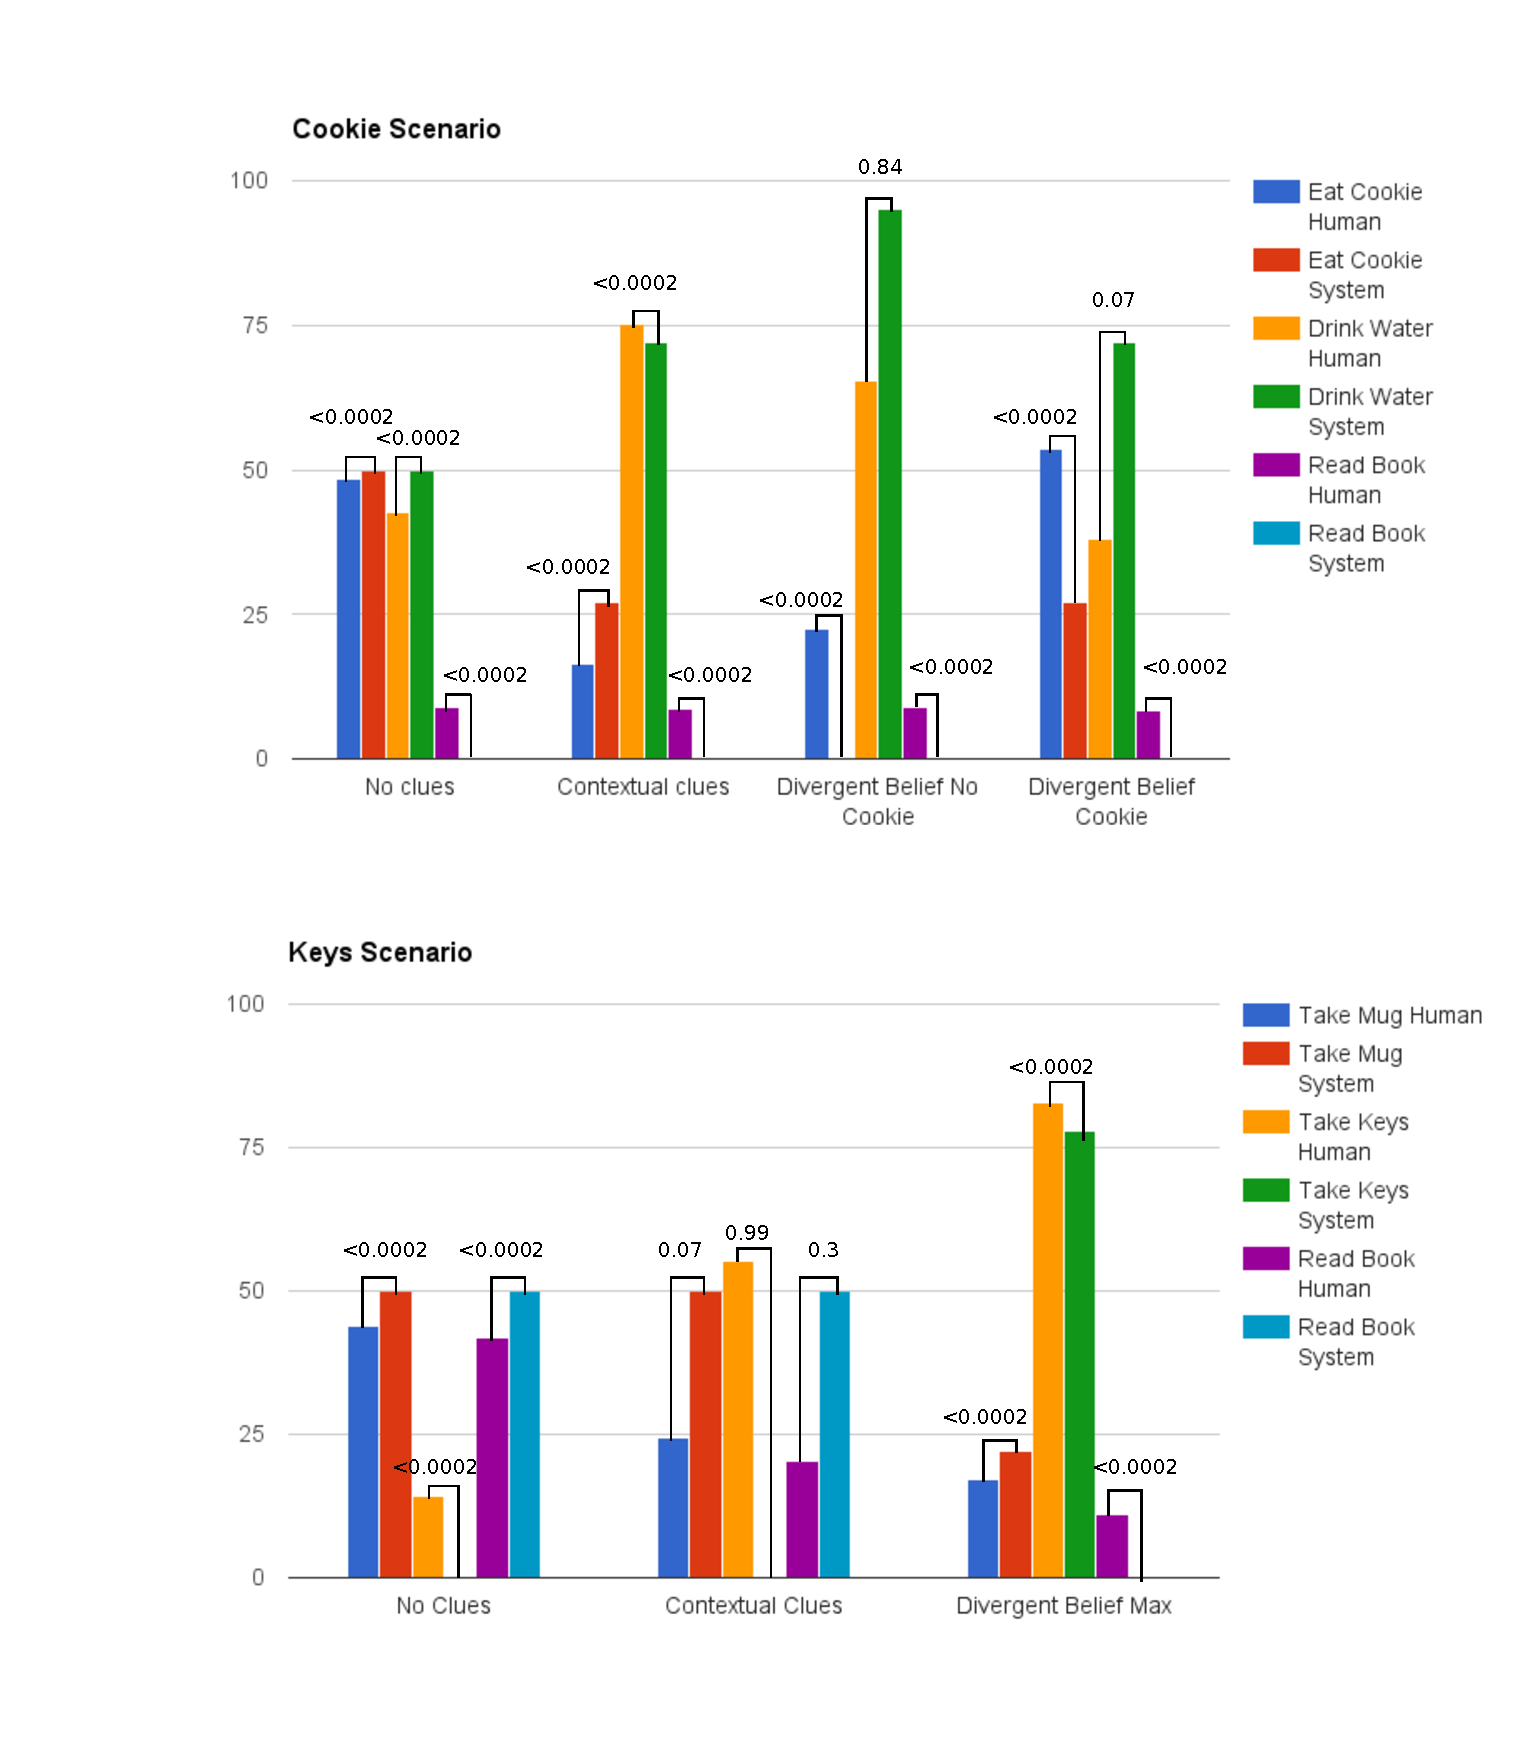
\includegraphics[clip,scale=0.7]{img/observer/scenarios_redone_1.pdf}
	\caption[Experiment results]{Experiment results. Results from the two scenarios are represented as graphs. Intentions, as estimated by the humans and the system, are represented by different colors, as shown in the legend of the graphs, with estimations of the same intention by the system or the human placed in adjacent positions. Each column represents the likelihood of an intention, expressed as a percentile score. P-values from the equivalence tests are shown, linking the estimation of an intention by the humans and by the system.}
	\label{fig:observer_experiments-user_study_results}
\end{figure}



 

\part{The Robot Coworker} % Main chapter title

\label{part:robot_coworker} % Change X to a consecutive number; for referencing this chapter elsewhere, use \ref{ChapterX}

\lhead{Part 2. \emph{The Robot Coworker}} % Change X to a consecutive number; this is for the header on each page - perhaps a

Robots can be used to perform a large number of different operations. Some of these will be simple enough that the robot can just achieve its task by performing a prefixed sequence of elementary actions. In other cases, the robot might have to achieve complex goals, which require the ability to create plans and to adapt them to the current state of the world. When cooperating with other agents, the robot has to build a shared plan, which includes the actions that every agent need to perform, in order to coordinate and ensure the correct achievement of the goal. We can imagine the following process:
\begin{itemize}
	\item The system receives a new goal. This can be directly introduced by a human, or chosen after some kind of reasoning by the robot.
	\item One of the agents (the robot or the humans) proposes a plan to achieve the goal, and presents it to the other agents.
	\item The agents negotiate the plan. In some situations, one of the agents might not be able (or might not want) to perform a specific action, or sequence of actions. The agent can refuse the plan, proposing a correction or a completely different plan.
	\item The agents execute the plan. Each agent performs its part of the plan. In addition, agents may check the state of others to monitor the correct execution of their part of the plan or to coordinate with them.
	\item An agent might fail its part of the plan. If this happens the agents need to create a new plan to account for this failure.
 	\item The process continues until the goal is achieved or it becomes unachievable (for example, a needed resource is no longer available).
\end{itemize}

When humans cooperate this process can be very quick. For simple tasks humans are able to coordinate without explicitly forming a plan, in particular if they are used to cooperating together. Other times, when there are unexpected problems during the execution of a plan, humans are able to quickly re-adapt their plan, without completely restarting this process. In order to cooperate in a natural way with humans, robots need to reproduce these mechanisms.

In this part we will introduce the mechanisms that we developed for the \textit{robot coworker} problem. In this problem, the robot has to achieve a goal together with a human, cooperating to solve the task. We are particularly interested in tightly coupled problems, where the agent and the robot need to interact often in order to achieve a goal.
The main aspects of our work are the management of plans, shown in chapter~\ref{chapter:plan_management}, and their execution, particularly the execution of joint actions, shown in chapter~\ref{chapter:task_execution}. Chapter~\ref{chapter:coworker_experiments} shows our experiments in the robot coworker problem. We also show, in chapter~\ref{chapter:mamdp} a recent extension to this work, involving multi-agent probabilistic planning.

% Chapter Template

\chapter{Plan Management} % Main chapter title

\label{chapter:plan_management} % Change X to a consecutive number; for referencing this chapter elsewhere, use \ref{ChapterX}

\lhead{Chapter 6. \emph{Plan Management}} % Change X to a consecutive number; this is for the header on each page - perhaps a shortened title

In this chapter, we introduce the Plan Management capacity of our system. Section~\ref{sec:plan_management-intro} introduces the subject, with a review of two systems able to manage cooperative plans. Section~\ref{sec:plan_management-overview} shows the main aspects of this component. Our system is able to use different plan management modalities, as explained in section~\ref{sec:plan_management-modalities}. Section~\ref{sec:plan_management-hatp} introduces HATP, a human-aware multi-agent planner interfaced with our system. Section~\ref{sec:plan_management-plan_manager} introduces our algorithm to manage plans. Finally, section~\ref{sec:plan_management-plan_monitoring} explains how we compare human activities with the current cooperative plan.

\section{Introduction}
\label{sec:plan_management-intro}

When agents cooperate, they agree on a common plan to solve the task, implicitly or explicitly. We call this sort of plan a \textit{shared plan}.  Participants in a shared plan do not limit themselves to simply execute their parts of the plan, but, in fact, need to constantly monitor other participants, to synchronize their actions and adapt their plans to them. Let us an imagine a situation where the robot is executing a shared plan with Greg. If the robot execute its own actions without observing Greg we might encounter several situation where the two will put in danger, perhaps even preclude, the achievement of the goal. For example, Greg might be late in executing a crucial action, and the robot should wait for him. An even more dangerous example happens if Greg has starts following another plan, for personal choice or for other circumstances, and does not inform the robot about this change. If the robot does not notice that Greg has changed his strategy, and does not adapt its own plan, the two might not be able to achieve their goal.

We call \textit{plan management} the process where the robot executes its own actions while coordinating with others and monitoring their activities. 

Two examples of systems able to execute shared plans are  Chaski \citep{shah2011improved} and Pike \citep{levine2014concurrent,karpas2015robust}.

Chaski is an executive system that enables the robot to anticipate and adapt to other agents actions. Chaski is based on human teamwork strategies, including ideas such as least moment commitment, frequent communications on the task status, and considering the consequences of the robot's choices on other agents. Chaski is able to execute plans in two different modalities: Equal Partners and Leader and Assistant. The system receives as input a shared plan, which includes the activities that need to be performed, the capacities of each agent, and the deadlines for these activities. Chaski produces a compact representation of all the possible schedulings of activities, based on this plan, which is used to take decisions on the fly during execution and to adapt to human choices. Results show that Chaski is able to reduce human's idle time in an equal partners scenario. A possible problem of this approach is that, if an agent completely deviates from the chosen plan, the system needs to create a new plan, which needs to be encoded again.

Pike is another executive, able to simultaneously recognize human plans and adapt to them. Pike receives as input a plan, represented as a Temporal Plan Network with Uncertainty (TPNU). Pike represents this plan by considering controllable choices (i.e. actions) for the robot and uncontrollable choices for the human. The idea is considering that these choices are not independent.  In this way the system can infer what actions the human would rationally take to achieve his goal and what actions the robot should take to help him. The system receives a stream of human choices, which allows it to determine the robot's actions. Pike has been tested in simulation and with a real robot with good results, managing, on average, to take decisions with a low latency.

If the human does not follow the TPNU Pike will return a failure. The authors discuss integrating the system with a generative planner in the future to overcome this limitation.

In the next sections, we will present our approach to the problem.

\section{Overview}
\label{sec:plan_management-overview}

\subsection{Process Overview}
Our Plan Management module receives, as input, a goal, which can be generated by the system or introduced by a human, using a tablet interface. After receiving a goal, the system will request a multi-agent plan to the task planner, including the actions of the robot and of other humans. We do not deal, in this module, with issues of task scheduling, which we leave to the task planner. While, in this chapter, we will concentrate on cooperative plans, our system is completely able to manage plans with only one agent, robot or human. 

One of the goals of our system is flexibility; we consider important the possibility to interface with external components. Different planners can interface with our plan management algorithm, if they respect our interface.

For each scenario, we define a planning \textit{domain}, which includes every entity and task that can be used in plans for that scenario. We consider that plans can be decomposed in a set of sub-parts, that we call \textit{tasks}. In general tasks can be further decomposed in simpler sub-tasks, until reaching the most basic form of task of a domain, which we call \textit{action}. Both actions and tasks follow the same representations, $(name,preconditions,target,postconditions)$, that we introduced in chapter~\ref{chapter:belief_management}. In chapter~\ref{chapter:intention} we introduced our intention and action recognition module. As we said, this this module possesses a list of known actions. Every action in a planning domain that can be performed by humans need to be present in this list. In this way, the system will be able to monitor the execution of actions by humans, by using the mechanisms of the robot observes. This process will be explained in more details in section~\ref{sec:plan_management-plan_monitoring}.

In some situations, to be more generic, we will use the word \textit{task} to refer to both tasks and actions, since actions are actually tasks that can not be decomposed in the current planning model.

Each planner used by our system needs to represent its plans as a set of streams, one for each agent. A stream is a sequence of nodes, where each node corresponds to task assigned to be executed by the agent. Nodes can be connected by causal links, even among different streams, to ensure synchronization. A causal link $l=(t_1,t_2)$ indicates that  task $t_1$ should be execute before task $t_2$. This ensures that all the preconditions to execute $t_2$ are fullfilled. Moreover, if $t_1$ and $t_2$ are executed by different agents, and if there is a shared resource connected to the task, the causal link indicates that the resource will be released by the agent only after $t_1$ is completed. An example of this data structure is shown in figure~\ref{fig:plan_management-streams}.

\begin{figure}[ht!]
 \centering
  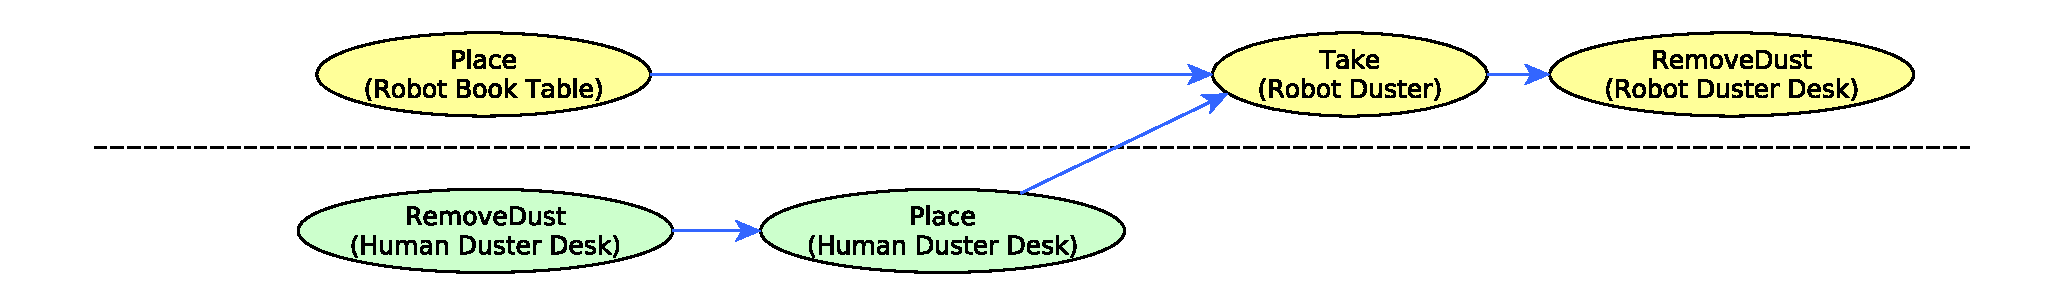
\includegraphics[scale=0.45]{img/coworker/plan_management/streams.pdf}
 \caption[Plan data structures]{
 A plan stream structure. The upper stream represents the robot, and the lower one a human. Each node represents a task to be performed by the agent. For each task, the stream shows its name and, in parenthesis, the name of the agent and the parameters of the task. Causal links are represented as arrows between the nodes. Notice the causal link between the Place(Human Duster Desk) node in the human stream and the Take(Robot Duster) node in the robot stream. This link indicates that the robot should wait that the human places the duster before executing the action to take it, ensuring synchronization.}
 \label{fig:plan_management-streams}
 \end{figure}

The system will manage each stream separately. By using the causal links, the robot is able to synchronize with humans. Joint actions (e.g. cooperative actions executed by two agents) will be treated by this module as actions of the robot, and be executed with a specific framework,  explained in chapter~\ref{chapter:task_execution}.

Plans can be managed in three different modalities. The robot can be the leader, choosing a plan and guiding the human in its execution. The robot can also be an assistant, and follow the orders of the human. Finally, the robot and the human can be equal partners. This mechanisms will be explained in section~\ref{sec:plan_management-modalities}.


% \begin{itemize}
% 	\item Interface with external planners in order to create a shared plan. The system has been integrated with a HTN (Hierarchical Task Network) based planner, HATP (Human-Aware Task Planner), and with a multi-agent MDP planner.
% 	\item Monitor a human plan. Our system is able to monitor other agents' parts of a plan, to cordinate with them and to react when an agent fails an action or his actions diverge from the current plan.
% 	\item Receive plans from a user. Users can interact with the robot with a tablet application, asking it to execute specific actions or goals.
% 	\item Executing shared plans in different modalities. The robot can be a leader, assistant, or equal partner of humans during plan management.
% \end{itemize}

\subsection{Architecture}
A number of modules implement these ideas, as shown in figure \ref{fig:plan_management-architecture}:
\begin{itemize}
\item Task Planner. Creates a shared plan for the involved agents. We consider the Task Planner as an external module. Our system has been integrated with the HATP planner, which we will introduce in section~\ref{sec:plan_management-hatp}. We have also recently introduced a probabilistic multi-agent planner based on MDPs, which we will discuss in chapter~\ref{chapter:mamdp}.
\item Plan Manager. Manages the current plan, interacting with the Task Execution layer to execute the robot's tasks and with the Situation Assessment layer to monitor humans' tasks.
\end{itemize}

After receiving a goal from the Goal Management layer, the Plan Manager module sends a request to the Task Planner to look for a suitable plan. After receiving a plan, this module will interact with the Task Execution and Situation Assessment layers to execute it. 

\afterpage{\clearpage}
\begin{sidewaysfigure}[ht!]
	\centering
	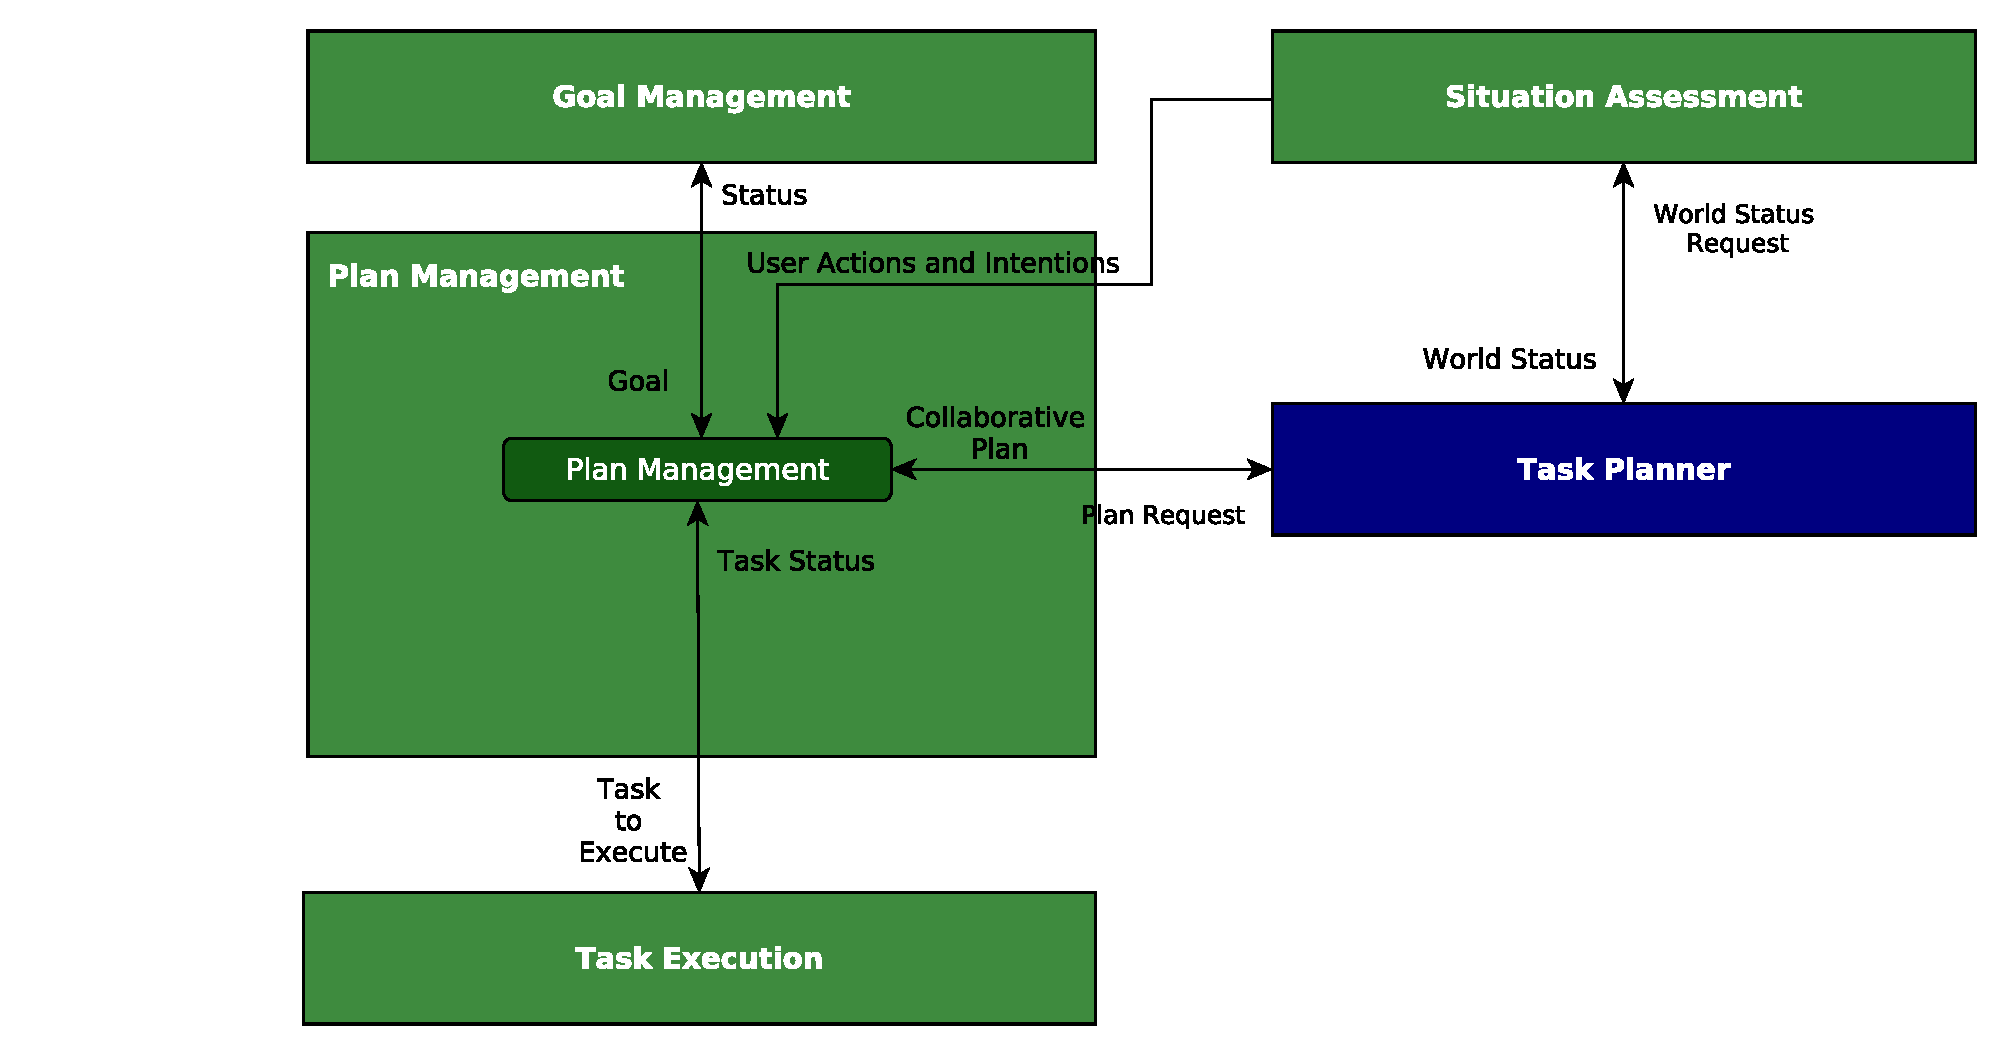
\includegraphics[scale=0.5]{img/coworker/plan_management/plan_management_architecture.pdf}
	\caption[The architecture of the Plan Management layer]{The architecture of the Plan Management layer. Light green rectangles represent modules, while dark green rectangles layers. The Task Planner is shown as a blue rectangle to indicate that it is a module external to the system. Arrows represent messages exchanged between components, with the label detailing the message.}
	\label{fig:plan_management-architecture}
\end{sidewaysfigure}


Parts of this chapter were presented in \cite{Lallement2014,fioreiser2014}.

\section{Plan Management Modalities}
\label{sec:plan_management-modalities}
When acting together, agents sometimes do not have the same decision power, with one of them assuming the role of a leader. We represent this idea, in our system, by proposing three different modalities: \textit{robot leader}, \textit{human leader}, and \textit{equal partners}. The robot is able to switch from one modality to another during the execution of a plan. For example, if the current modality is \textit{robot leader} and rhe Robot receives a command from a user, it will switch to the \textit{human leader} modality, after interrupting its current action.

\subsection{Robot leader}
\label{subsec:plan_management-robot_leader}
In this modality the robot, after computing the plan, will present it to the user and start executing it. The robot will track the status of humans, informing them of which actions they should execute. This modality can be helpful when interacting with  naive users or in tasks where the robot has a better knowledge of the  domain or of the environment than the other agents.

We have developed two different algorithms to present the computed plan to the user. In the first, simpler case, the robot will verbalize sequentially all the actions, stating which agent should perform them. 

For example, the plan presented in figure~\ref{fig:plan_management-streams} would be explained in the following way: ``I will place the book on the table. You will remove the dust from the desk and then place the duster on the desk. After that, I will take the duster and then I will remove the dust from the desk".

To generate this kind of verbalization we create a textual representation for each object and task, and then verbalize it with a text-to-speech application. Using simple rules, we follow the plan streams and verbalize each node. To create a more interesting and varied explanation, we use some connective words between nodes. We added some randomness in the algorithm. For example, the robot will randomly select words such as ``At this point", ``After that", or ``Then" to introduce a task. Since this algorithm is not a focus of our work we will not present it in details.

 We have also developed a more advanced algorithm to adapt this process to the expertise of a user in the tasks to execute. We will present this algorithm in chapter~\ref{chapter:knowledge}.

\subsection{Human Leader}
The human can also create plans, interacting with the robot by using a
tablet application, shown in figure~\ref{fig:plan_management-tablet}. Using the tablet, the human can choose a goal for the robot, but also pause or stop its actions. The human can choose, as goal,  the execution of a simple action, but also of a more complex task, involving many actions.


In this modality the robot  will simply observe the surroundings and wait for user inputs. User commands have a priority over the other two plan management modalities. If the robot receives a command from the
application while it is in another modality, it will abandon its current
plan, stopping its actions at a safe point, and then execute the user's
command. 

We feel that this interaction modality is important for two
different reasons.  First, some users will simply prefer to be in
charge of the execution process, for a matter of personal preference or because they
feel they have a deeper knowledge on how to realize the current task
than the robot. We can picture, for example, industrial or medical
scenarios, where the human is the leader and asks the robot to perform
different tasks to help him, when needed.

 A second use of this modality is in situations where
the robot does not have  a clear estimation of the users' intentions and
goals. For example, in a domestic environment, a user could decide to
order a robot to bring him a drink, a need that the robot can not always anticipate.

\begin{figure}[ht!]
 \centering
 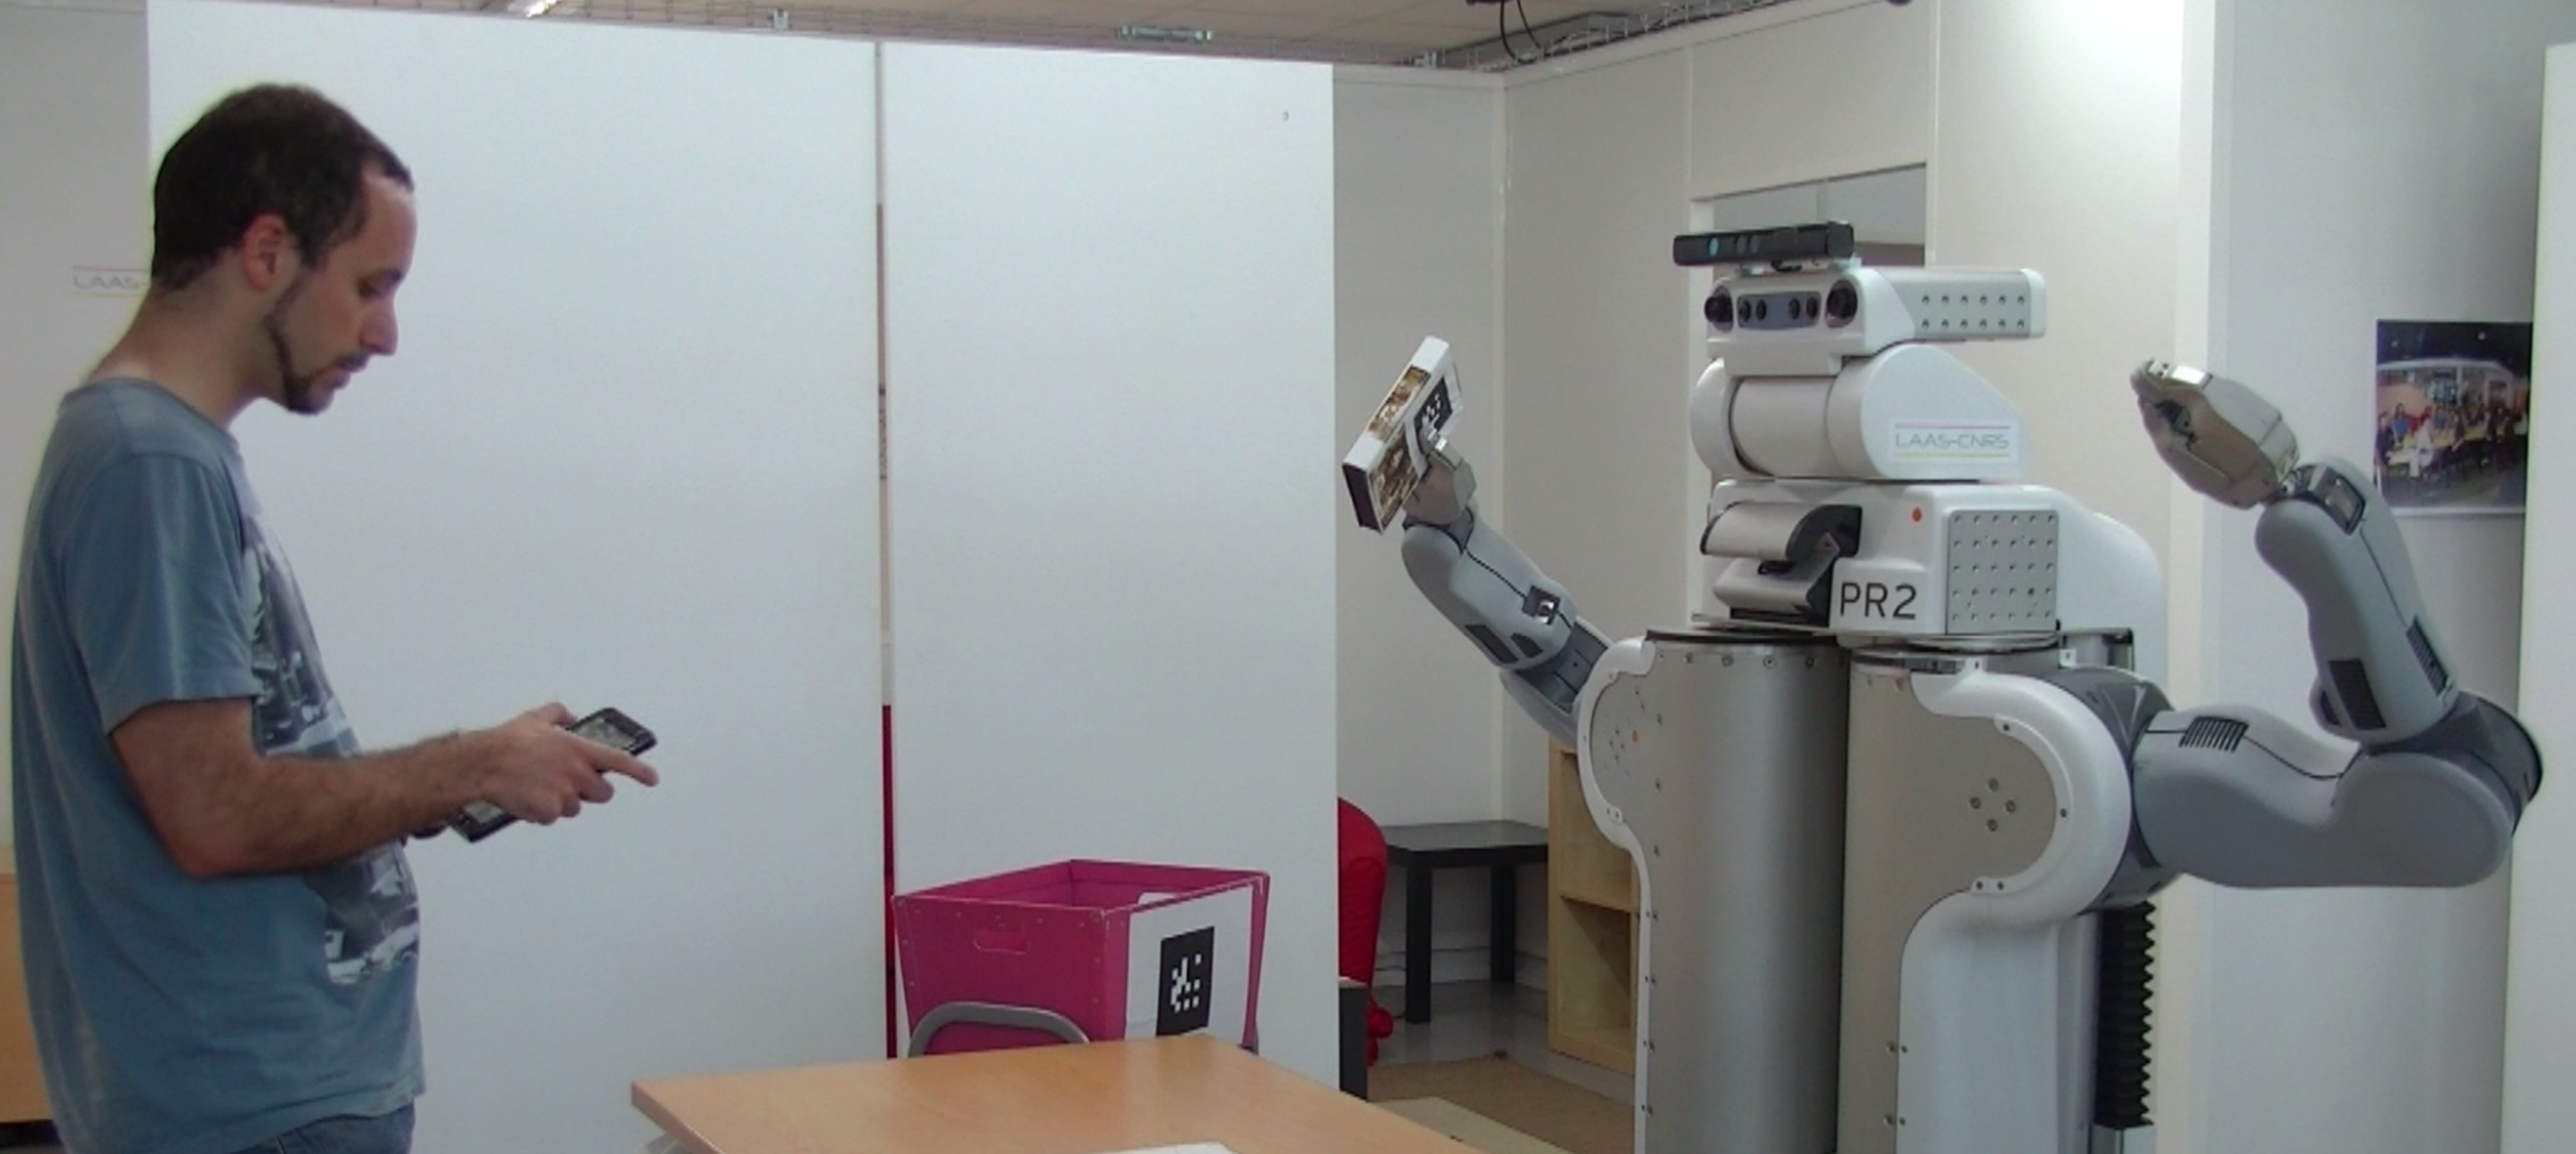
\includegraphics[scale=0.25]{img/coworker/plan_management/tablet.pdf}
 \caption[Giving goals to the robot]{The human is giving a goal to the robot by using a tablet application.}
 \label{fig:plan_management-tablet}
 \end{figure}

\subsection{Equal Partners}
In the last presented operation modality the robot will try to help
the human to complete a task. At the start of the scenario, the robot
will observe the environment. After the user takes an
action the robot will calculate a plan and try to help as it can, by
performing actions related to that task and by giving helpful information to
the user, for example to fill gaps in their knowledge. In this modality, 
the robot will not explain or negotiate the current plan and will not warn humans if
their actions differ from the plan computed by the robot.

We feel that, particularly in non-critical tasks, where defining an accurate plan between the partners is not
fundamental, this modality is a very natural way of
interaction between different partners.



\section{Human-Aware Task Planner}
\label{sec:plan_management-hatp}
In this section we will briefly introduce HATP~\citep{Lallement2014}, a planning framework that we used in many experiments with our system.

Computing a plan in complex environments can be very hard and time consuming. A useful approach to reduce the search space in planning is introducing the knowledge of an expert in the system, in order to guide the planner toward desirable states. An implementation of this idea is Hierarchic Task Network (HTN), where the domain expert specifies a hierarchical library of operations, called methods, when the operation is a node in the hierarchy, and actions, when the operation is a leaf. HATP extends HTN for human-robot interaction problems. Among the capacities of HATP we can find:
\begin{itemize}
\item Multi-Agent. HATP is able to include different agents in its domain, specifying which actions each one can execute. HATP is able to plan for different agents at the same time, humans and robots. The planner can also compute ``joint actions", that involves more agents at the same time.
\item Social Rules. The domain expert can introduce a set of rules, which represent desirable behaviors. Social rules help producing human-aware plans, that avoid behaviors that can be considered rude for humans. Using social rules, HATP can also balance in different ways the amount of effort of each agent in the plan. For example, we might choose that the human should have a minimum effort in the plan, or that the effort should be balanced between the human and the robot.
\item Cost Driven. The domain expert can specify a cost for actions. Plan pruning allows to explore more efficiently the search space, discarding paths that are not promising.
\end{itemize} 

Plans are represented as an HTN tree decomposition and as a set of streams, one per agent, which shows which actions each agent needs to perform. Causal links are introduced between streams to ensure synchronization.

\section{Plan Management}
\label{sec:plan_management-plan_manager}

Our plan management algorithm receives as input a plan composed by a set of streams, one for each agent. Each stream will be handled in parallel, using different threads of execution. We will now explain this algorithm, which is shown in figure \ref{fig:plan_management-manage_plan}.
\begin{itemize}
  \item Each thread executes the part of the plan of an agent, composed by $n$ different tasks.
  \item For each task, for every causal link $(t_i,t_n$), where $t_n$ is the current task, and $t_i$ is another task, the plan manager waits until $t_i$ is completed, or there is an error. This process is handled in the \textit{waitCausalLinks} procedure.
  \item When all the causal links have been satisfied, the execute\textbackslash monitor procedure is called, depending if the thread is managing the robot or a human. The \textit{executeTask} operation interacts with the Task Execution layer to complete the task, while the MonitorTask operation with the Situation Assessment layer.
  \item If these procedures succed, the Plan Manager switches to the next task, otherwise it returns a failure.
  \item The process is continued until there is a failure or the plan for the current agent is completed.
\end{itemize} 

\begin{figure}[ht!]
 \centering
 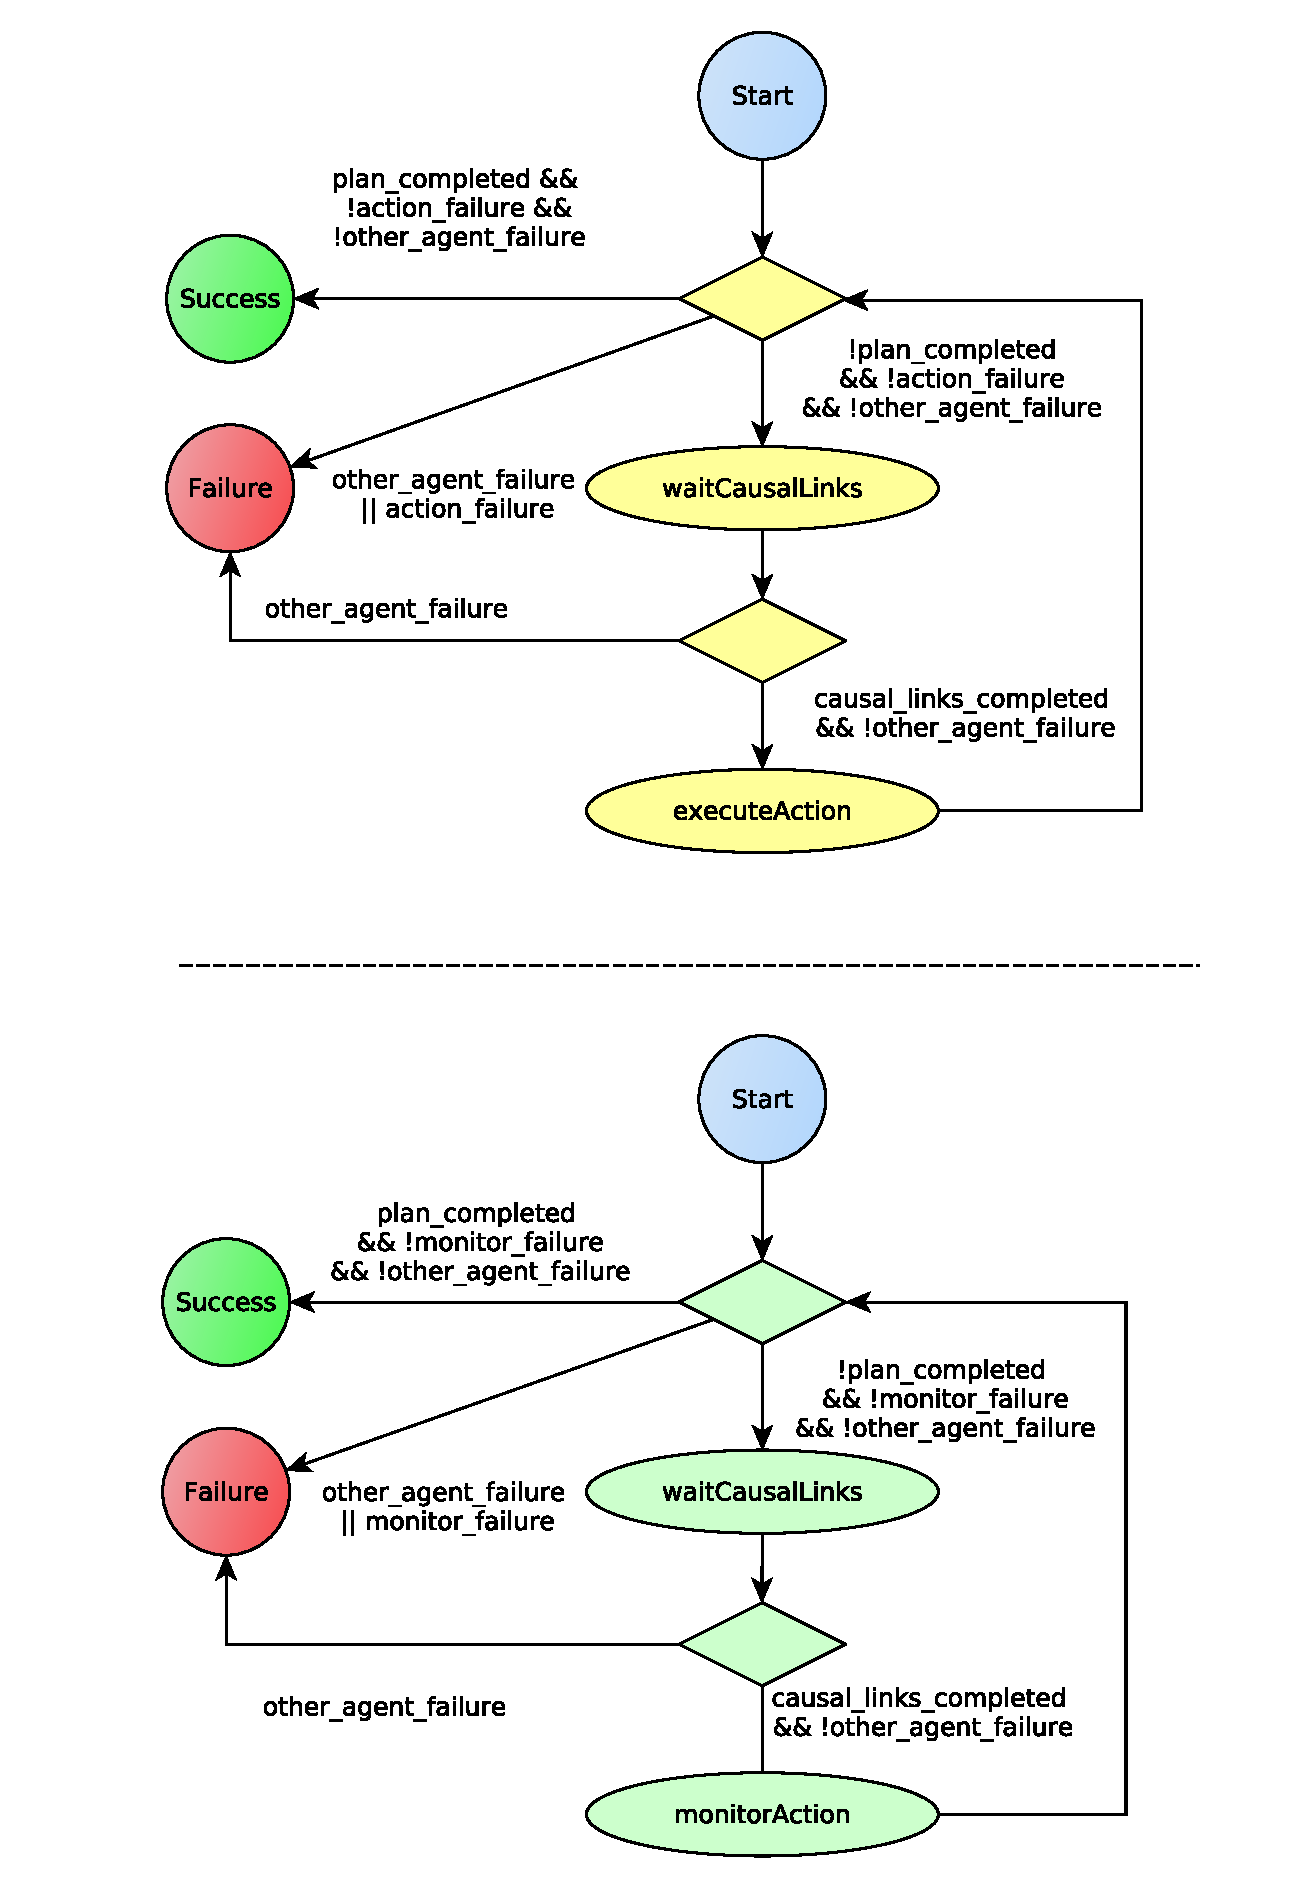
\includegraphics[scale=0.6]{img/coworker/plan_management/manage_plan.pdf}
 \caption[Plan Management Algorithm]{The plan management algorithm. The algorithm is composed by different threads, one for each agent. In this instance, the upper lane represents the robot's management thread, while the bottom a human's management thread. Elliptic nodes represent operations. Diamond nodes, representing divergences in the algorithm, where added to the graph only when they could simplify the understanding of the algorithm. Arrows imply a transition between nodes, with the label of the arrow representing the condition of the transition, when present. The absence of a label implies that a transition is always applied. The blue circle node, called ``start", represents the start of the algorithm. The green and red circle nodes, instead, represent the success or failure of the algorithm.}
 \label{fig:plan_management-manage_plan}
 \end{figure}

Failures in the algorithm lead to a replan request. If a new plan is found, the algorithm starts again, otherwhise the goal is considered as failed. Depending on the modality, the robot will also give different verbal information to the human.

If the current management modality is \textit{robot leader}, the robot will warn the human the he executed a wrong action. If the replan is successfull, the robot will explain the new plan to the human. 

When the human is the leader, the robot is following orders. The current order might be to execute a task which still requires coordination, and the robot might expect the human to follow a particular strategy. If the human deviates from this strategy the robot will replan, but not issue any warning.

A similar approach is used in the \textit{equal partners} modality. In this case, the robot will adapt to the deviations in the humans' actions, but the replanning process should be almost hidden from the human, in order to be more natural. The robot will replan and start managing the new plan without informing the human.

% In this modality, the robot will expect users to execute a specific set of tasks, warning them if they do not respect this allocation. Sometimes, the robot will choose the decomposition of the tasks that should be executed by a user, but, when the partner is competent enough in a high-level task,  we may want to allow him the flexibility to execute it as he sees fit. 

\section{Task Monitoring}
\label{sec:plan_management-plan_monitoring}

During the execution of a plan, the robot will monitor other human partners. In general, having a shared plan, the robot knows what is the next task that the human should perform, and can monitor if it is accomplished. Task monitoring poses a number of different issues:
\begin{itemize}
\item Understanding when the next expected action has been performed. In some situations the robot will monitor the execution of a specific action. In this event, it needs to understand when the action has been completed.
\item Understanding when the next expected task has been performed. In some situations, the robot wants to give a human cooperator the freedom to perform a task (that is, a complex operation that can be composed by a sequence of actions) as he sees fit. This is a more complex problem than monitoring a specific action, since the robot needs to reason on the results of sequences of actions.
\item Evaluating the human engagement in the current task. The robot needs to understand if the human is trying to accomplish its current task, if he momentarily interrupted it, or if he abandoned it.
\end{itemize}

At the moment, we have implemented and integrated in our system only monitoring of actions. We will show how we include this idea, and then illustrate in the chapter~\ref{chapter:mamdp} how we could extend our system to monitor tasks and evaluate the human engagement in the current task.

\subsection{Monitoring Actions}
At all time, as previously explained in chapter~\ref{chapter:intention}, the robot constantly observes the environment, monitoring which actions are executed. As previously said, each action that can be executed by a human needs to have the same representation in the Situation Assessment and Plan Management layers. When the Plan Manager needs to monitor an action $a$ of a human stream, its $preconditions$ will be satisfied (since, if we are monitoring $a$, all of its causal links have been already satisfied). This means that $a$ will be present in the IG for the human, which will be monitoring its execution (chapter~\ref{chapter:intention} gives more details about this mechanism).

As we said in section~\ref{subsec:intention-unknown_intentions}, the single-agent MDP mechanism that we introduced is not sufficient to monitor a joint goal, and so the IG for the human, in the coworker scenario, only includes Actions and Observation nodes.

The Plan Manager will wait for Situation Assessement to infer that an action has been performed by the human. If the action is different from $a$, it will return an error, prompting a replan. Otherwise, the plan management will continue with the next action in the stream, if there are any.

For example, let us imagine a scenario where Greg is near a table, with a \textit{bottle} and a \textit{book} on top. Let us say that, at the moment, Greg can execute three actions: \textit{take book}, \textit{take bottle}, and \textit{move kitchen}. The current IG for Greg will include these actions, as well as observations to infer their execution. In this example, Greg's plan is represented by a stream of three sequential actions: \textit{move to table, take bottle, move kitchen}. 
Greg has just completed the action \textit{move to table}, and should now execute the action \textit{take bottle}, if he follows this stream. If the system infers that Greg executes \textit{take book} or \textit{move kitchen}, the plan manager will replan, since Greg executed a different action that the one that was expected. If Greg executes \textit{take book}, the system will start monitoring the next action in the stream, which is \textit{move kitchen}.


\subsection{Monitoring and Unseen Actions}
Often, in cooperative tasks, agents will operate in different locations, and so they can not observe each other actions all the time. Perhaps one of the agents is cooking in the kitchen,  while the robot is preparing the table for dinner. While we do not deal, in this work, with these issues, there are several studies on plan recognition in partially observable environments, like \cite{geib2005partial}. 
% Chapter Template

\chapter{Task Execution} % Main chapter title

\label{chapter:task_execution} % Change X to a consecutive number; for referencing this chapter elsewhere, use \ref{ChapterX}

\lhead{Chapter 7. \emph{Task Execution}} % Change X to a consecutive number; this is for the header on each page - perhaps a shortened title

This chapter shows how our system is able to execute tasks, and particularly joint actions. Section~\ref{sec:task_execution-intro} introduces the subject. Section~\ref{sec:task_execution-overview} describes our approach, with the components that implement it. Section~\ref{sec:task_execution-action_executor} shows the main aspects of the Task Executor module, while section~\ref{sec:task_execution-collaborative_planners} shows the framework we use to execute human-robot joint actions. Finally, section~\ref{sec:task_execution-handover} shows an example of a Collaborative Planner for human-robot handovers.


\section{Introduction}
\label{sec:task_execution-intro}
Acting in a human-crowded environment is a difficult problem. Even when acting independently, the robot needs: to ensure human safety, by taking others into account when planning and stopping if its actions could bring harm; to perform legible movements, so that its actions can be understand by humans (studied, for example, in~\cite{dragan2013legibility}); and to be robust, trying to complete its task even in front of unexpect conditions. 

These issues show us that humans should not be treated as simple obstacles by the robot, but need specialized reasoning and execution algorithms.

When performing a cooperative action with the human the robot needs to continuously monitor its partner, checking if he is involved in the task, stopping to wait for him, adapting its movements, and eventually abandoning the task. For example, if the robot is giving an object to a human, it will have to choose a position for its arm where the human can easily reach the object, change this position if the human is moving, and abandon the task if the human leaves the area.

\cite{bussy2012proactive} studied how to execute a transportation scenario jointly with a human partner, but the work is based more on haptic and control issues than actual reasoning, an area of the problem not deeply investigated.


\section{Overview}
\label{sec:task_execution-overview}

\subsection{Process Overview}

We have built a module to execute tasks, represented, as in the previous chapter, as $(name, preconditions, target, postconditions)$, in a human-aware way. The focus of this module is not the planning or execution of the robot's motions, which are handled in external components, but the  execution of a task, from start to finish. This problem presents several issues and steps:

\begin{itemize}
\item The robot needs to monitor if the task is actually achievable. Even though, if the task is part of the plan, our plan management algorithm, presented in section~\ref{sec:plan_management-plan_management} ensures that the preconditions of the task are satisfied when it is executed, the task could still not be executable. This problem may arise for different reasons. First, the robot is planning by using its knowledge of the state of the world, which may be faulty. For example, the robot might believe, when planning, that an object is on a table, and produce a plan where it will take it. If the object's location was different, because it was moved without the robot knowing, the robot will not be able to achieve its task. Second, external events can happen that make a task unachievable. The robot might not be able to detect or link these events to the achievement of a task. For example, if a gush of wind throws the object to the floor, the robot might not immediatly understand that this will prevent it in the future to take the object.
\item The system needs to interact with motion planners and executors to produce the range of movements needed by the robot to achieve its action.
\item The robot needs to constantly monitor its environment in order to ensure that the action is executed in a safe way. In particular, humans may move, while the robot is acting, in positions where they could be endanger by the robot's motions. To ensure human's safety, the robot needs to detect these situations and stop or pause its motions.
\item After a task is executed, the system needs to infer its effects, in order to update the knowledge on the state of the world. In general, a part of the postconditions of the actions could be observed by the robot. For example, if the robot has placed an object on a table, the robot could observe, and not only infer, its location. Since our perception can be faulty, if we do not integrate observation with inference, we might encounter situations where the robot is not able to observe the effects of its actions. For example, the robot has placed an object on the table, but the light conditions or the orientation of the object do not allow it's recognition by the perception algorithms. To avoid this problem, the robot will update the position of the object using inference, in its mental model, and then refine it through observation, if it is able to see it.
\end{itemize}

We are particularly interested in the execution of human-robot joint actions. We have defined, in chapter\~ref{chapter-overview} a joint action as a cooperative action between the two agents. As previously said, this kind of action requires additional mechanism to allow the robot to cooperate with the human in a natural and efficient way. We developed a specific framework, which we called Cooperative Planners, based on MOMDPs, to deal with this issue, which we explain in section~\ref{sec:task_execution-cooperative_planners}

\subsection{Architecture}

These ideas are represented in the following modules, as shown in figure~\ref{fig:task_execution:architecture}.
\begin{itemize}
	\item Task Executor. This module executes the robot's actions in a robust, human-aware, and flexible way.
	\item Collaborative Planners. This set of planners are used to execute human-robot joint actions, allowing the robot to adapt its actions to the collaborators.
	\item Motion Planners and Executors. These planners, treated as external modules, are in charge of choosing trajectories for the robot, taking into account the environment and the present agents. We will not discuss this component, as it is outside the boundaries of this work. More details can be found in \cite{Sisbot2008,Mainprice2011,Pandey2010}.
\end{itemize}

We developed this layer with flexibility in mind. We can easily expand the system, by adding new actions, or switching motion planners and executors, without having an impact on the rest of the architecture.

\begin{figure}[h!]
	\centering
	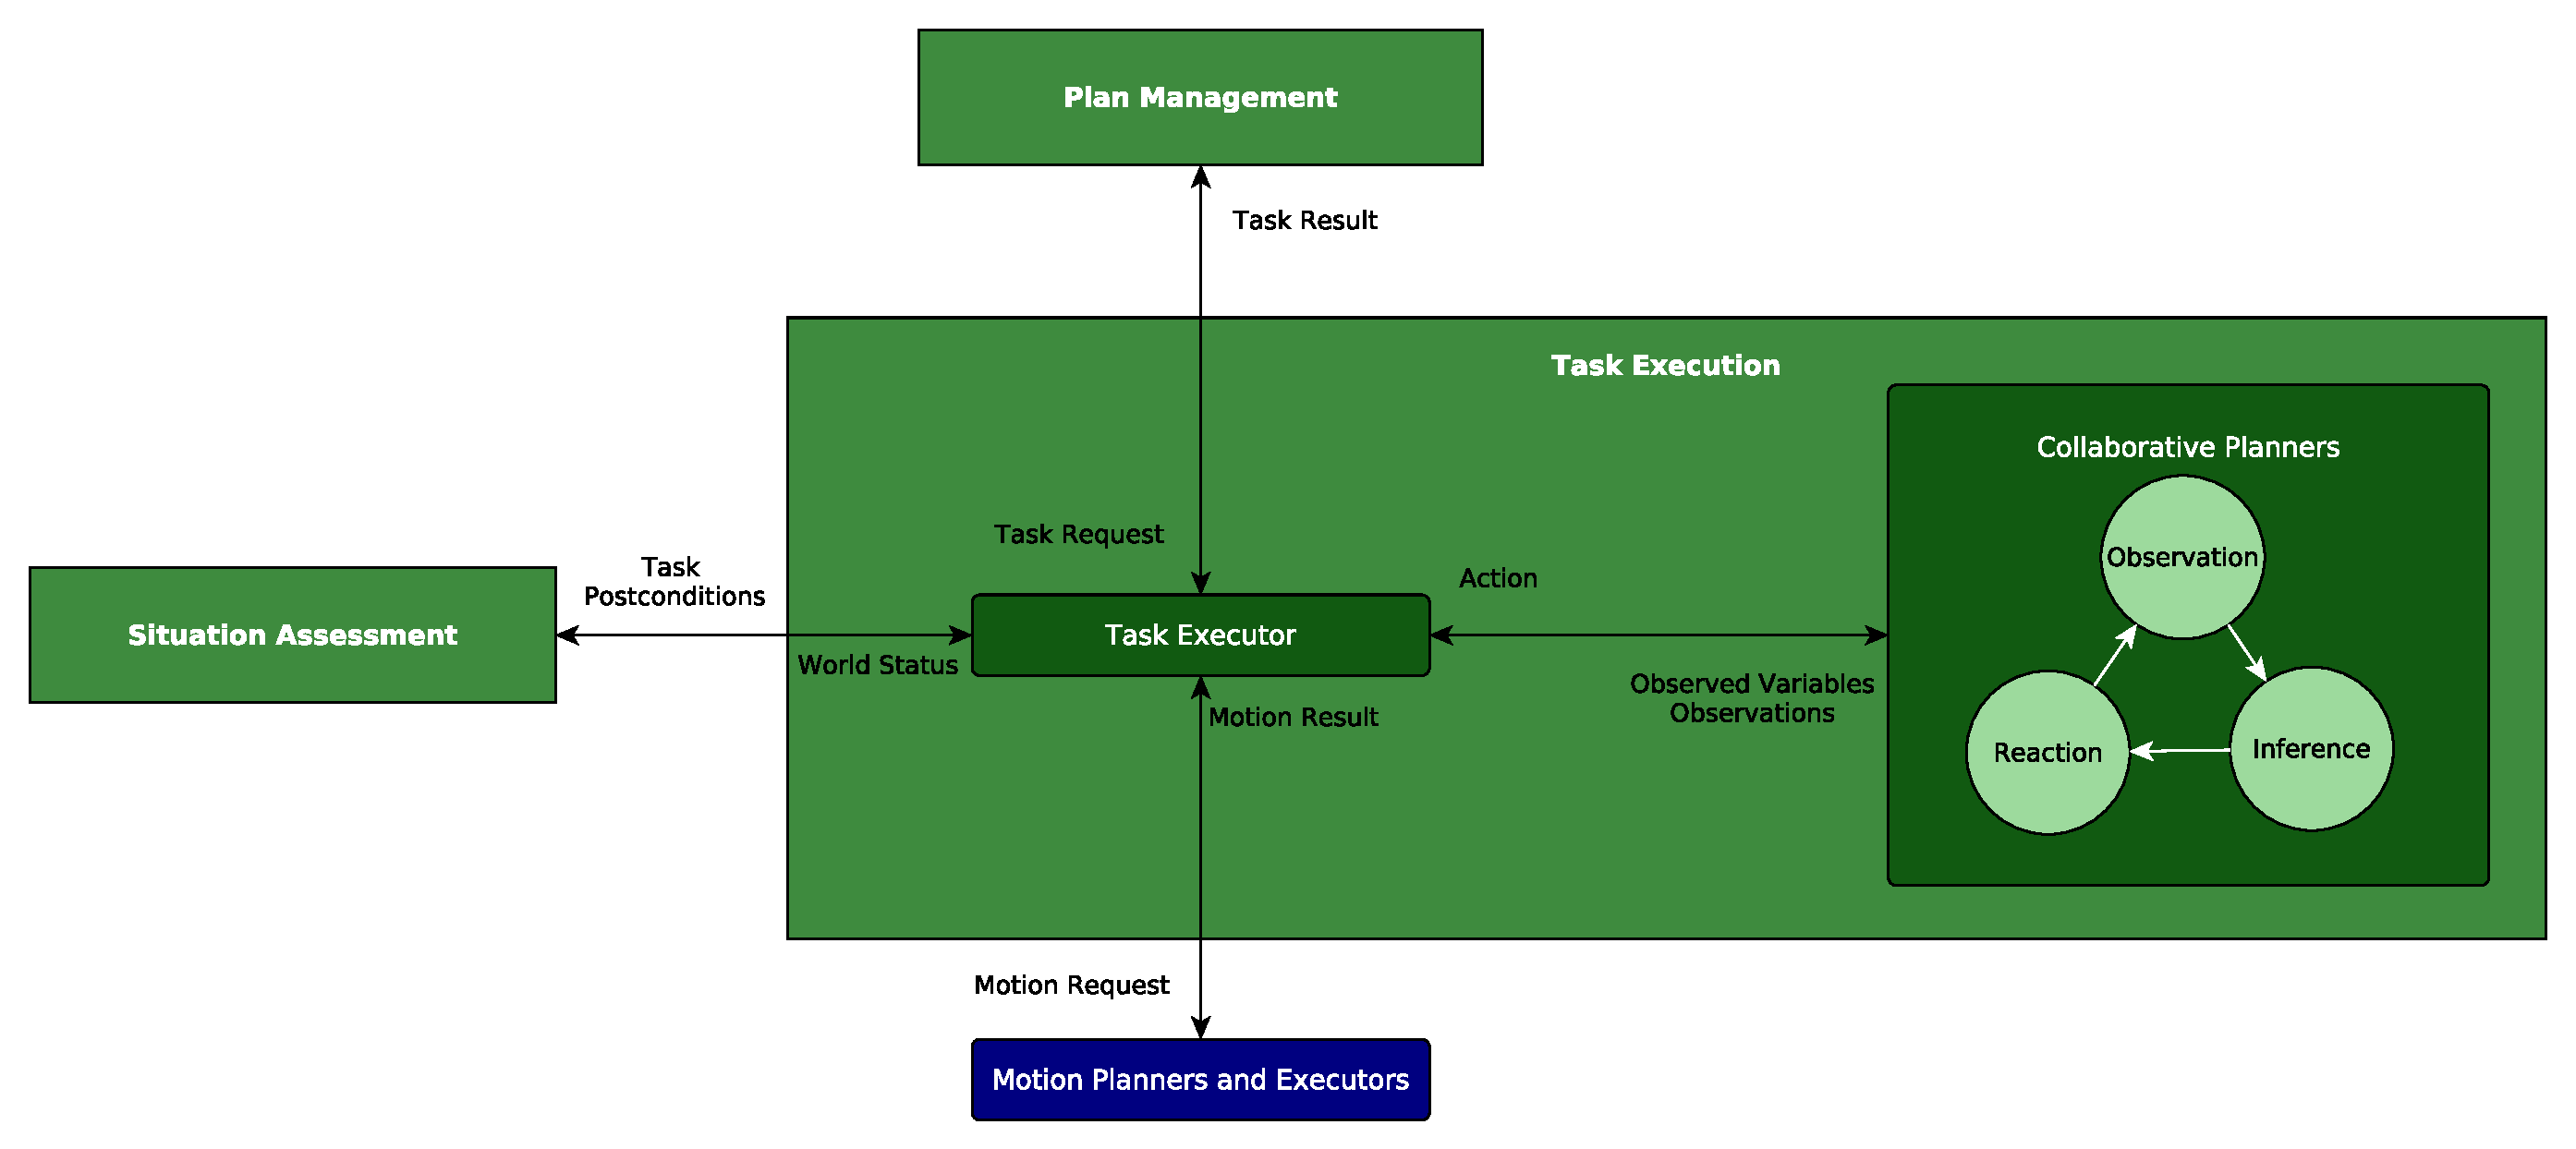
\includegraphics[clip,scale=0.38]{img/coworker/task_execution/architecture.pdf}
	\caption[The architecture of the Task Execution layer]{The architecture of the Task Execution  layer. Dark green rectangles represent modules, while light green rectangles layers. Blue rectangle repreesent external modules. Arrows represent message exchanged between components, with the label detailing the message. The white ellipses represens, and their arrows, represent the process of the Collaborative Planners, explained in Section \ref{sec:task_execution-collaborative_planners}. While, in this image we present the Collaborative Planners as a single unit, the system actually has a set of planners, and will choose, during the execution of a joint action, which one to use.}
	\label{fig:task_execution:architecture}
\end{figure}


Parts of this chapter where presented in~\cite{fioreiser2014}.

\section{Task Executor}
\label{sec:task_execution-action_executor}
The Task Executor handles task requests from the Plan Management layer. Following the ideas presented in section~\ref{sec:task_execution-overview}, the execution of an task is handled in several steps:
\begin{itemize}
\item Check Preconditions. The system can check if the preconditions of the task are valid by sending a query to the Situation Assessment layer. If the preconditions are not valid, the module returns an error.
\item Execute Task. The task is executed, by communicating with the Motion Planners and Executors and, if the current task is a joint action, with the Collaborative Planners.
\item Set Postconditions. The postconditions of the task are set in the Situation Assessment layer.
\end{itemize}

The execution of an task can fail, and in that case the world status is updated consequently. For example, if the robot was trying to pick an object, and the motion planner does not manage to compute a trajectory to reach it, the object will be considered as \textit{not reachable} by the robot in the current world status. When the Plan Management replans, the system could look for a plan where the robot changes position and tries again the pick, or even asks another agent to give him the object.

Tasks can be paused and resumed, for example because a human steps in the trajectory planned by the robot. The robot is also able to show some social clues during an action, for example by moving its head toward the tasks's $target$. 

\section{Collaborative Planners} 
\label{sec:task_execution-collaborative_planners}
When executing joint actions with humans, the robot needs to continuously observe its partner and react appropriately. The robot's action should be based on different aspects. First of all, the robot should act differently depending on the current status and level of advancement of the task. Second, the robot should consider the status of the world, in order to take appropriate actions. Then, as we said, the robot should observe its partner's behavior, which can give different information. Of course, the robot should coordinate with the human's movements. For example, if the two agents are performing an handover, and the human extends his hand, the robot should extend its arm to bring the object in a reachable position.

Observing the human's action can give us more subtle information, that represent how much he is engaged in the task. For example, in the case of the handover, if the human is oriented toward the robot and extending his hand, we can assume that the human is currently engaged and cooperating. If, instead, the human is looking in another direction, or moving away, we can infer that he is currently doing something else, and perhaps has even abandoned the task.

To reason on all these variables and produce an appropriate reaction, we introduced a special framework to manage cooperative actions, called the Collaborative Planners, based on hierarchical Mixed Observability Markov Decision Processes (MOMDP). A MOMDP can be modeled as a tuple $(S_h,S_o,A,T,R,\Omega,O,\gamma)$, where $S_h$ is the hidden state, $S_o$ is the observed state, $A$ is the set of actions, $T$ is the transition function, $R$ is the reward function, $\Omega$ is the observation function, $O$ is the set of observations, and $\gamma$ is a discount factor. More details about Markov Models are provided in chapter~\ref{chapter:appendix}.

Using an MMODP we can model both observed variables, like the task and world status, and hidden variables, like the engagement level of the human, which we can measure from observations. Using a hierarchy of models, as explained in \cite{pineau2001hierarchical}, we can represent complex scenarios and tasks with smaller, simpler models, that can be solved more easily, and expand them by adding more actions and complex behaviors as we see fit.

For each joint actions, we will introduce a new Collaborative Planner. When the system is executing a joint action between the robot and a human, the task executor will contact the related Collaborative Planner.  The task executor will send requests containing the observations and observed variables, used to update the MMODPs, and the planner will return a sub-action to execute. To maintain this model generic the Collaborative Planners will output high-level actions, which the task executor will adapt to the current situation. This process will continue until the planner reaches a goal states, chooses to abandon the task, or there is a failure.

We provide a \textit{basic framework} that we use to implement Collaborative Planners, that can be adapted to the specific task. While it is not obligatory to implement a Collaborative Planner following these ideas, we believe that they offer a good basis for cooperative tasks:

\begin{itemize}
	\item $S_h=\{human\_commitment\}$
		\begin{itemize}
			\item $values(human\_commitment)=\{engaged,not\_engaged,not\_interested\}$.
		\end{itemize}  

		The human commitment to the task can be modeled as a hidden variable.  A user can be engaged in the task, meaning that he is actively participating; not engaged, meaning that he is currently not participating, but we expect that he will resume the task (imagine, for example, a user receiving a phone call while executing a joint task); or not interested, meaning that he has abandoned the task. 

		Modeling the human commitment is very important, since the robot should choose its action based on this variable, and of course on other task related variables. For example, if the user is not currently engaged in the task, the robot might choose to wait for him, or ask him if he has a problem. If he has abandoned the task, the robot might look for another plan, or ask the help of another human. If he is committed, the robot could proceed to accomplish the task, as long as the world state allows it.

	\item $S_o:\{task\_advancement\}$.
		\begin{itemize}
			\item $values(task\_advancement)=\{not\_started,started,completed\}$.
		\end{itemize}

		The status of advancement of the task can provide useful information to help the robot to choose its actions. A simple way to represent it, is considering just an initial state, where the agents have decided to execute a cooperative task, but have not started executing it yet; a middle state, where the agents are working to complete the task; and a final state, where the task is completed. Different tasks could further refine this variable.
	\item $A:\{continue,wait,abandon,engage\}$.

		When building an action set, the developer should consider how much control the MOMDP should have over the robot's actions. In our implementations, we chose to plan generic high level actions, that will be adapted by the Task Executor. This strategy allows us to simplify the state space of the MOMDP. In a basic Collaborative Planner, the robot is able to: continue its task, meaning that it will take the next logical action depending on the current state, maintained by the Task Executor; wait for the user, if the robot detects that he is momentarily not engaged in the task; abandon, if the user is not interested anymore in executing the task; engage, to communicate with the user, for example by giving him a warning.

	\item $T$, $R$ and $O$ are, of course, completely dependent on the joint task.
	$\Omega$ is dependent on the current application. Some typical observations are related to spatial relationships between the user and the robot (e.g. the user is more likely to be interested in the task if he is close to the robot and oriented toward him), or particular poses of the user (e.g. the user is ready to receive an object if he has extended its arm toward the robot).

\end{itemize}

Our idea is similar to the work of \cite{ferrari2015hierarchical}. The authors propose a framework based on hierarchical POMDPs for cooperative tasks, with a three layer structure. This framework was applied to an escort application, where the robot had to guide a user to its location in a human-aware way, adapting to his behaviors. In this application, the commitment of the user is estimated by reasoning on how much the human is focused on the robot, and on their distance.
We implemented a similar application, for a robot guide, using our Collaborative Planners, which we will show in chapter~\ref{chapter:spencer}. The main difference between our framework and the one developed by the authors is that they chose to have a much richer decision power to the POMDP, while in our system planning is actually split among several units, and the Task Execution module has a big role in adapting the actions of the Collaborative Planners. We also do note use a precise hierarchical framework, leaving to the single Collaborative Planners the choice on how many layers of task to use.

We will show, in the next section, an example of collaborative planner which develops on this basic framework.

\section{Collaborative Planner for Handover}
\label{sec:task_execution-handover}
The handover collaborative planner has the goal to handle both human-robot and robot-human handovers in a human-aware way. We will show parts of this model now, avoiding the observation and transition function, as they are extensive and do not provide particular help in understanding this example.

\begin{itemize}
	\item $S_h:\{human\_commitment\}$.
		The hidden variable, and its values, follow the basic framework presented in the previous section.
	\item $S_o:\{task\_advancement\, timer, human\_distance\}$.
		\begin{itemize}
			\item $value(task\_advancement)=\{not\_started,started,touching,completed\}$.
			\item $values(timer)=\{not\_expired,expired\}$.
			\item $values(human\_distance)=\{close, far, out\_of\_range\}$.
		\end{itemize}

		The task advancement is represented in a similar way as the basic framework. We add the $touching$ value to this variable, representing the fact that the gripper of the robot has detected some pressure (e.g. the human has placed an object in it, if the handover is human-robot, or he has grabbed the object kept in the gripper, if the handover is robot-human).
		 We add a timer variable, which is started and controller by the Task Executor when the robot is waiting for the user, because he is momentarily not engaged in the task. When the timer expires in the Task Executor, this variable will be set accordingly, and the robot can perform specific actions (e.g. ask the user if he still wants to perform the task).
		 We also consider the human distance from the robot, classyfing it as $close$ to the robot, $far$ from the robot, and $out\_of\_range$ if the human is not visible. 
	\item $A:\{continue,wait,abandon,engage\}$.

		The actions follow the basic framework. The $continue$ action is chosen when the user is $engaged$. The Task Executor will react differently to this action, dependingly on the current $task\_advancement$. If $task\_advancement \neq touching$ then the robot will extend (or keep extended) the arm toward the user. If $task\_advancement=touching$ the robot will release the object, or grab it from the human's hand, depending on the kind of handover.

		The $wait$ action is chosen when the user is $not\_engaged$. In this case the robot will retract its hand to an intermediate position. The Task Executor will start a timer.

		The $abandon$ action is chosen when the user is $not\_interested$ or the task is $completed$.

		Finally, the $engage$ action is chosen when the $timer$ is $expired$. In this case the robot will ask the human if he still wants to perform the handover.
	\item
	\item $O:\{human\_arm\,human\_orientation,human\_distance\_variation\}$.
		\begin{itemize}
			\item $values(human\_arm)=\{approaching,retracting,still,unknown\}$.
			\item $values(human\_orientation)=\{toward\_robot,other,unknown\}$.
			\item $values(human\_distance\_variation)=\{decreasing,increasing,still,unknown\}$.
		\end{itemize}

		We present several human observations, used to estimate his engagement. In general, we consider that the human is more likely to be $engaged$ when he is approaching the robot, he is turned toward it, and his arm is extending. If the human is turned away, or even leaving, it is more likely that he is currently $not\_engaged$ or even $not\_interested$. Finally, if the human is $out\_of\_range$, his observations will be $unknown$, since the robot does not know his location.

	\item  $R$: the robot is rewarded for completing the task, performing the handover, and for executing desirable behaviors, like waiting for a user if we detect that he is not engaged, and abandoning the task if he is no longer interested in the joint action. 
\end{itemize}

An example of handover using this Collaborative Planner is shown in figure~\ref{fig:task_execution-handover}.

\begin{figure}[h!]
	\centering
	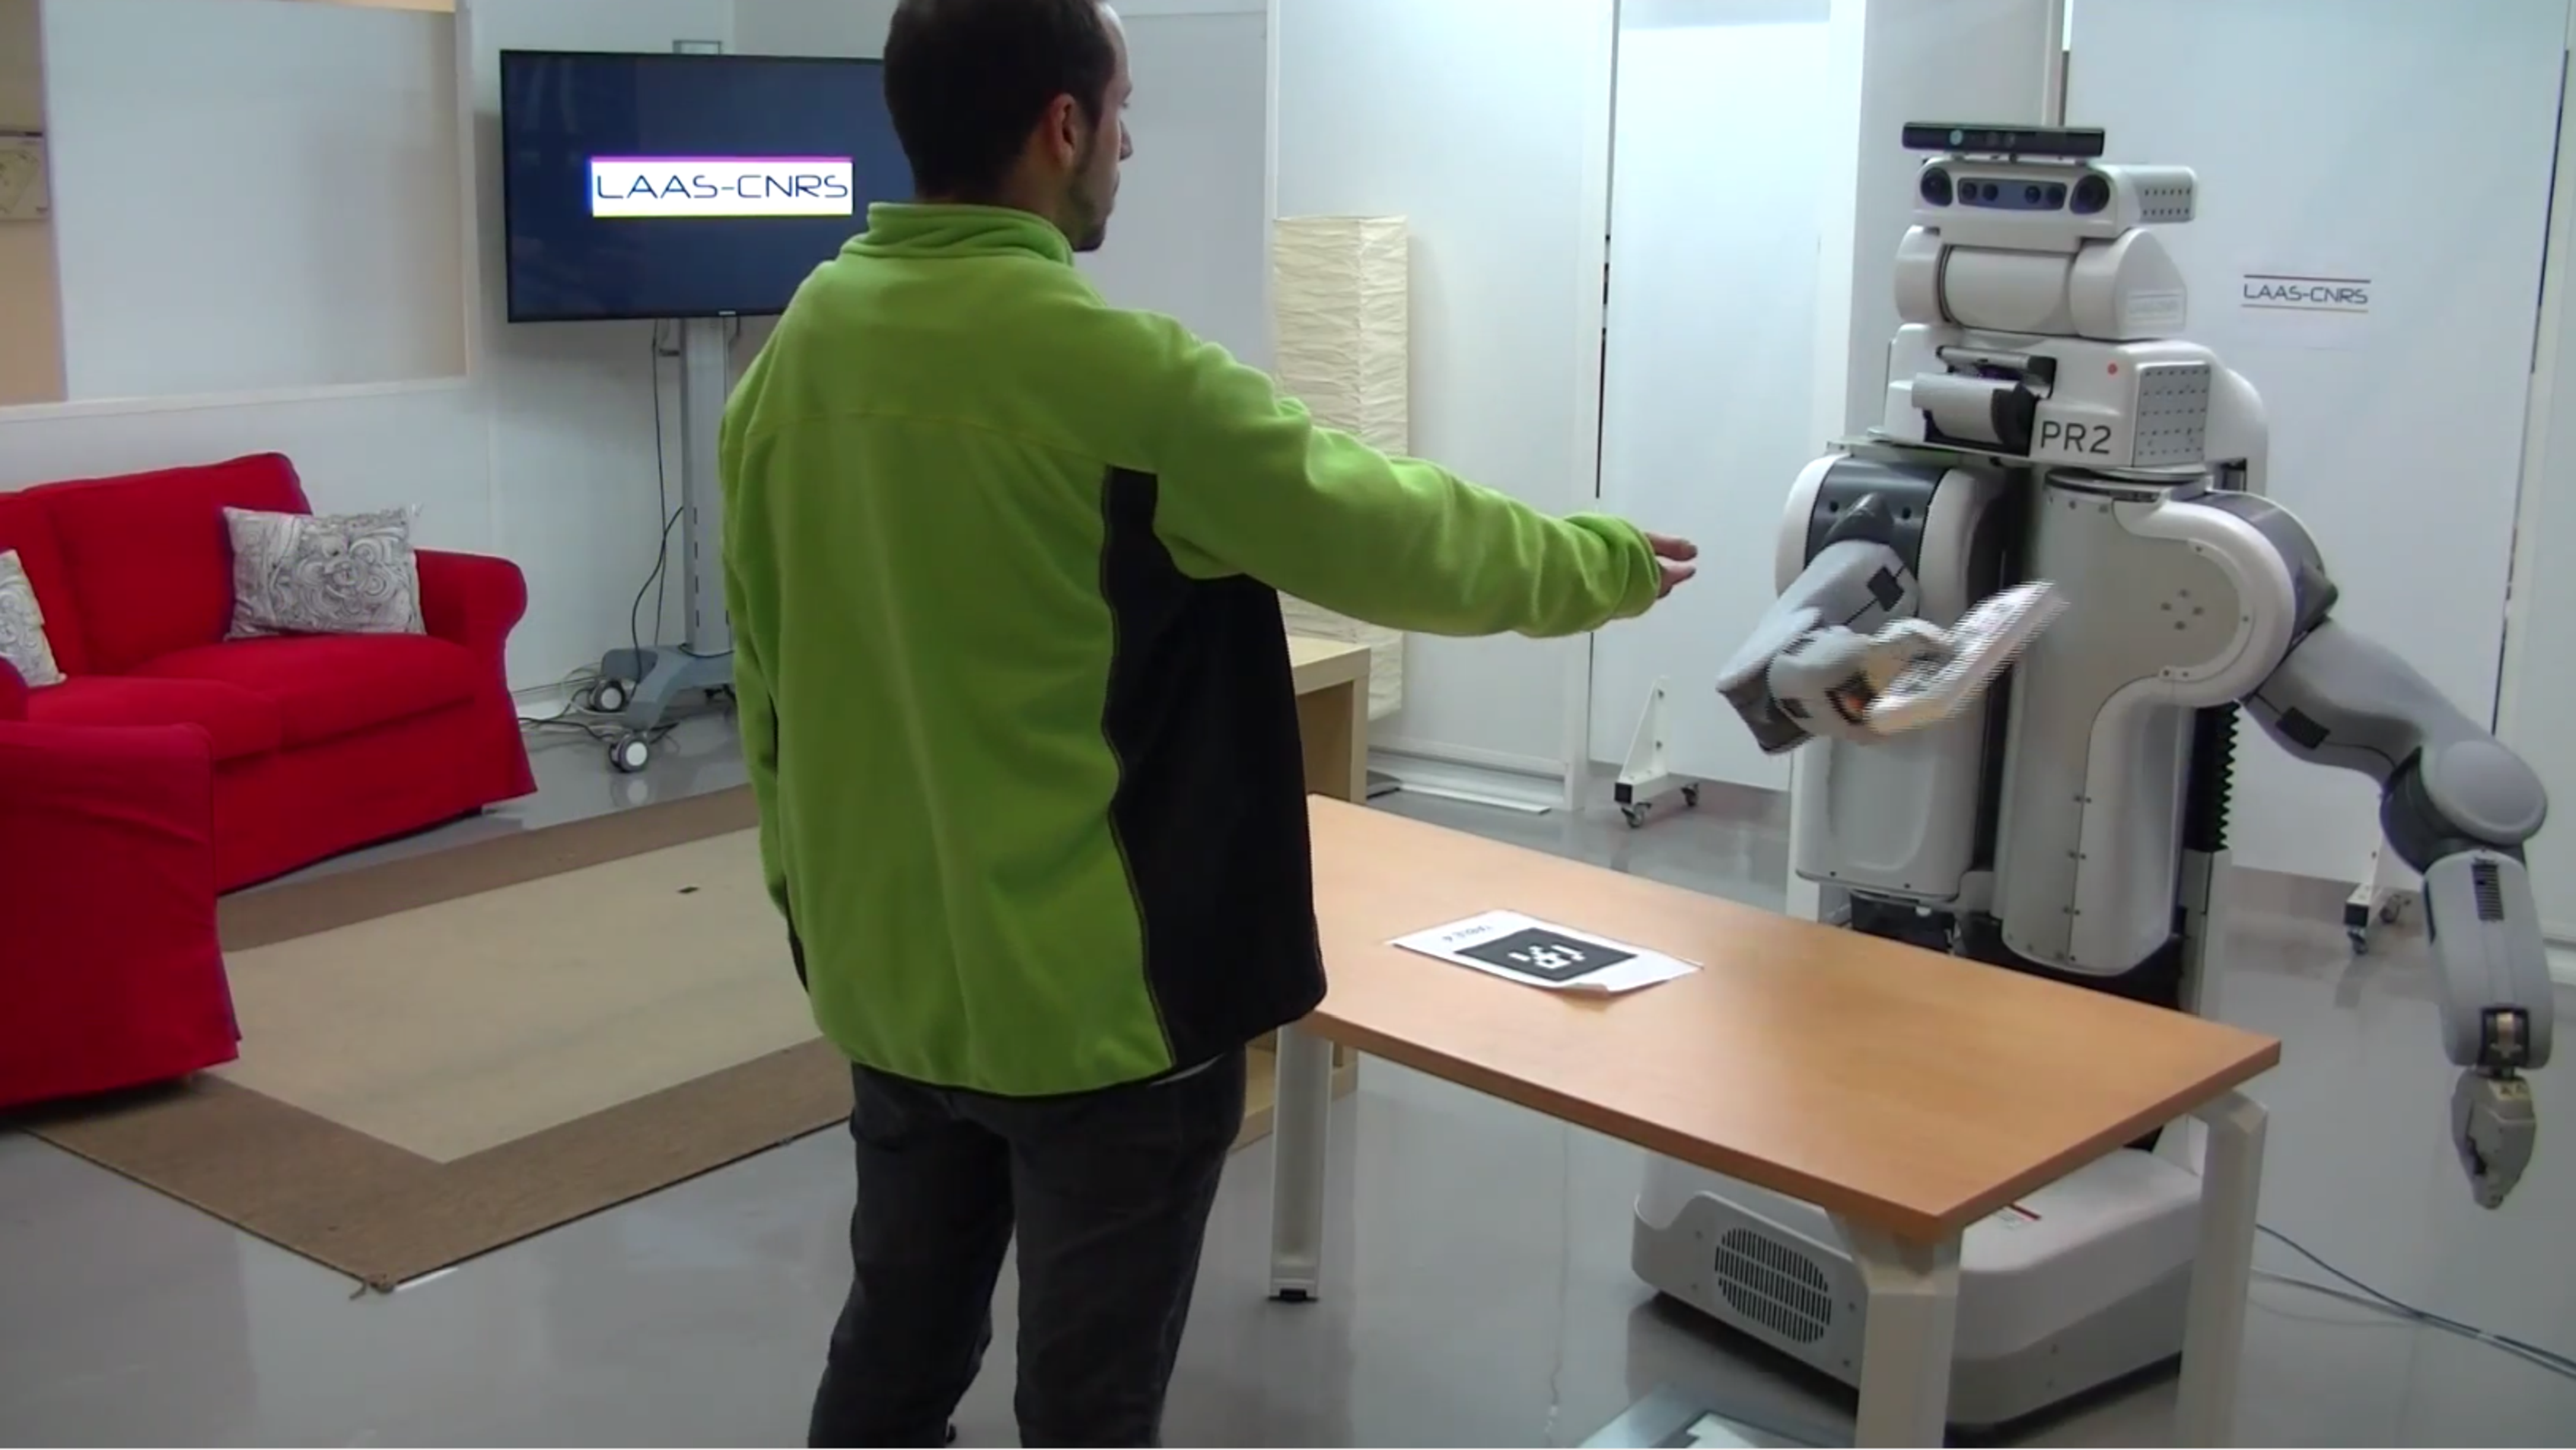
\includegraphics[scale=0.3]{img/coworker/task_execution/handover.pdf}
	\caption[Handover]{A robot-human handover}
	\label{fig:task_execution-handover}
\end{figure}
 
\chapter{Experiments and Results} % Main chapter title

\label{chapter:coworker_experiments} % Change X to a consecutive number; for referencing this chapter elsewhere, use \ref{ChapterX}

\lhead{Chapter 8. \emph{Experiments and Results}} % Change X to a consecutive number; this is for the header on each page - perhaps a shortened title

This chapter presents an experiment used to evaluate the robot coworker problem. Section~\ref{sec:coworker_experiments-scenario} introduces our scenario. Section~\ref{sec:coworker_experiments-experiment} shows our experiments. Finally, section~\ref{sec:coworker_experiments-discussion} presents and discusses our results.


\section{Scenario Description}
\label{sec:coworker_experiments-scenario}
In this section we show experiments created to validate our system in a domestic scenario, where the robot can help a human partner to achieve a joint task. This experiment was previously presented in \cite{fioreiser2014}.


We present a scenario where the robot, a PR2 by Willow Garage, and a human have a joint goal: cleaning a set of furniture. 
The environment is composed by two different furniture, a $TABLE$ and a $SHELF$, and three tapes,
 $TAPE1$, $TAPE2$ and $TAPE3$. The goal of the agents is throwing each tape in a $BIN$. We will present different examples, where the items will be placed differently, depending on our needs. The scenario is shown in figure \ref{fig:coworker_results-pr2helper}.

 \begin{figure}[ht!]
 	\centering
 	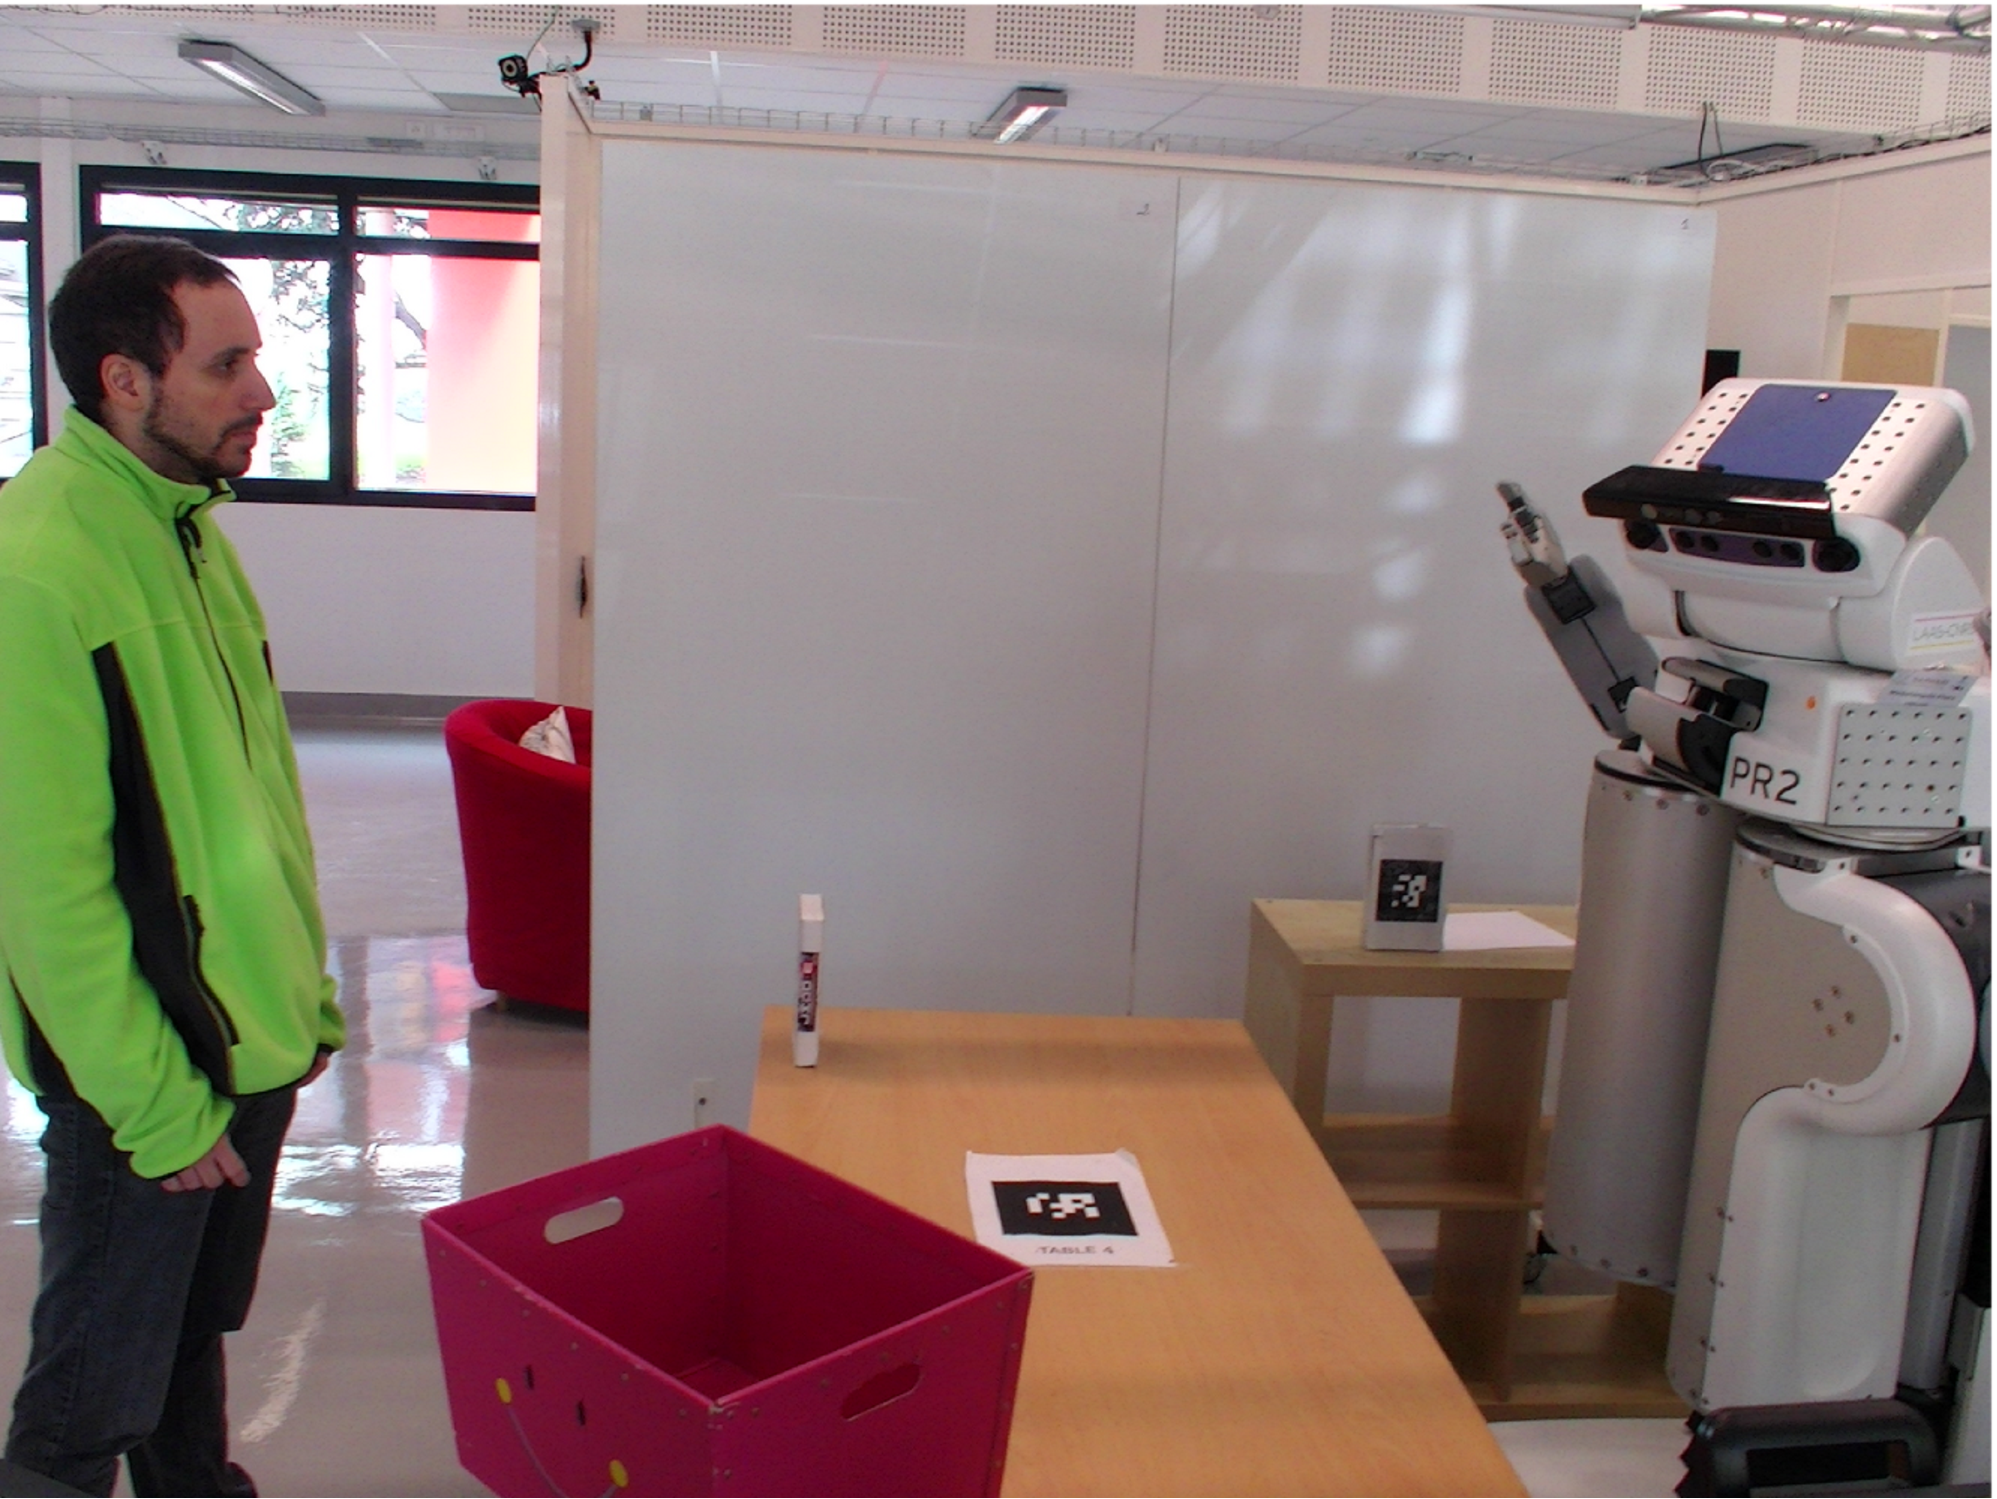
\includegraphics[scale=0.45]{img/coworker/results/experiment.pdf}
 	\caption{The robot coworker scenario example, with a PR2 robot and a user.}
 	\label{fig:coworker_results-pr2helper}
 \end{figure}

In this scenario, human detection and handling was done using a depth camera, mounted on the ceiling. the scenario uses both the capacities of the robot coworker, described in this part, and the belief management and action inference capacities of the robot observer, shown in part~\ref{part:robot_observer}.

\section{Experiments}
\label{sec:coworker_experiments-experiment}
We will describe different experiments conducted in our laboratory.

\begin{itemize}
  \item
\textbf{Equal Partners}.
In this scenario (figure \ref{fig:coworker_results-scenario1}) the user is asked to clean the table, without being explained what is the shared plan that will be used. The user is just informed that
the robot will try to help as it can to perform the task. The robot is already aware about the joint goal, but at the start of the scenario limits itself to monitor its partner. The user moves to the table and takes the \textit{TAPE2}. At this point, the robot infers that the user
has completed an action.
\begin{figure}
  \caption[Robot coworker experiment 1]{Robot adapts. This figure shows the robot's representation of the scenario. The white tape is the \textit{TAPE2}, while the blue
    one is the \textit{TAPE1}. The spheres represent the agents'
    rechabilities, with red spheres representing robot reachabilities
    and green spheres human reachabilities. In this case only the human
  can reach the \textit{TAPE2} while both agents can reach the \textit{TAPE1}
and the \textit{BIN}. After the human takes the \textit{TAPE2} the
robot produces a plan where the human must throw the tape in the
bin while the robot can take the \textit{TAPE1} and throw it in the
bin.
}
\centering
  \subfigure{
  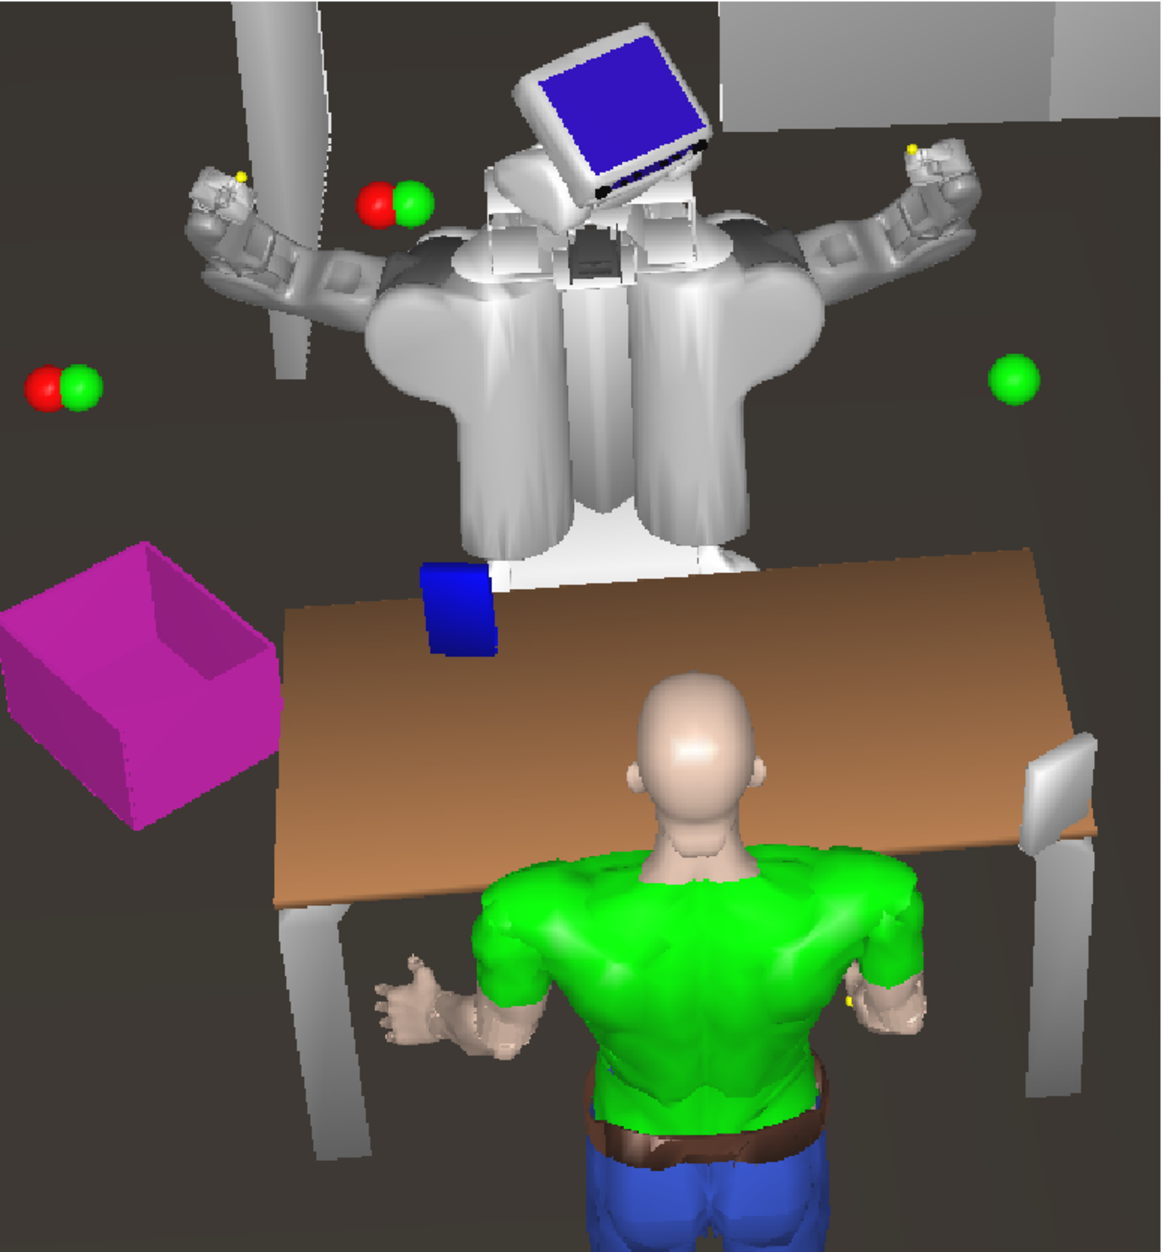
\includegraphics[scale=0.25]{img/coworker/results/scenario1.pdf}
  }
  \subfigure{
  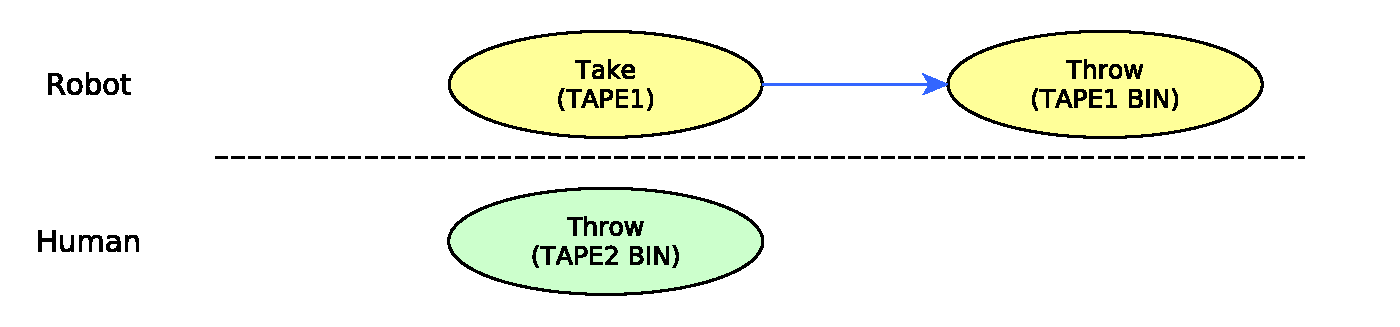
\includegraphics[scale=0.7]{img/coworker/results/plan1.pdf}
  }
  \label{fig:coworker_results-scenario1}
\end{figure}

The robot creates a plan and executes its part of it while monitoring the human,
who executes his part without deviating from the plan calculated by
the robot.

\item
\textbf{Modality switch and user plans}.
In this scenario (figure~\ref{fig:coworker_results_scenario2}) the robot is the only agent able to reach both tapes, but it can not reach
the bin, which can instead be reached by the human. We tested
this scenario in two different runs. In the first run, the current plan management modality is \textit{robot leader}.
After exploring the environment, the robot produces a plan and starts its execution.

\begin{figure}
  \centering
  \caption[Robot coworker experiment 2]{Modality switch and user plans. Another configuration of
    the environment, where the robot can reach the two tapes and the
    human can reach the bin. The robot generates an initial plan
  from this situation. The block surrounding the Give and Receive
  actions means that they are considered a single joint action.}
  \centering
  \subfigure {
    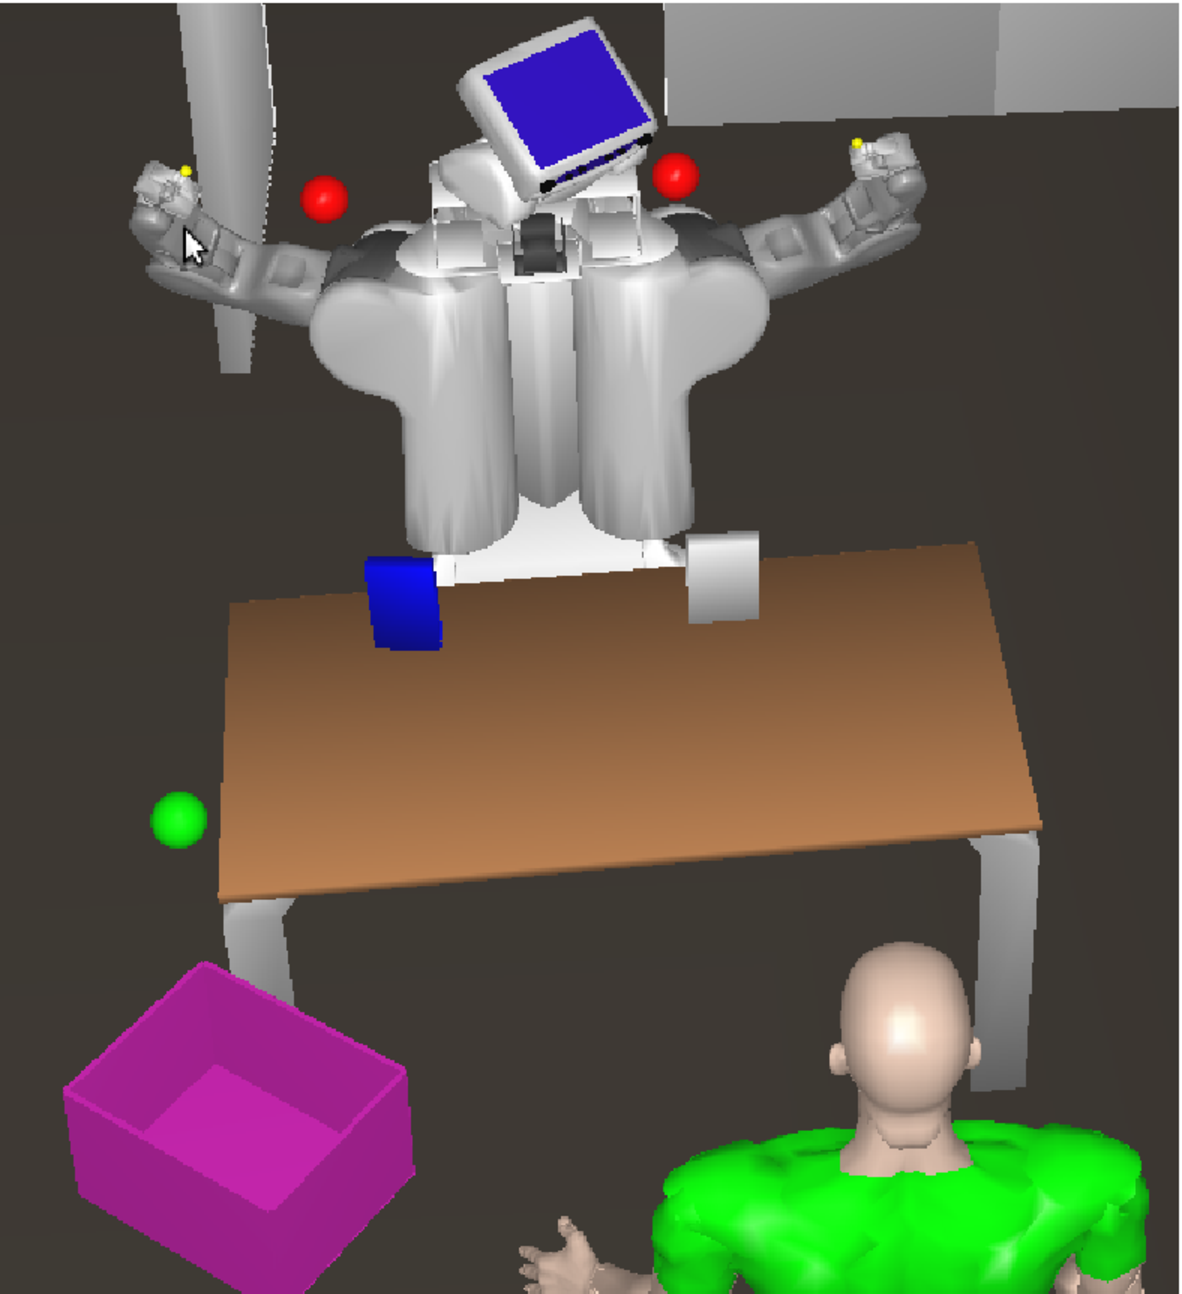
\includegraphics[scale=0.25]{img/coworker/results/scenario2.pdf}
   }
  \subfigure {
    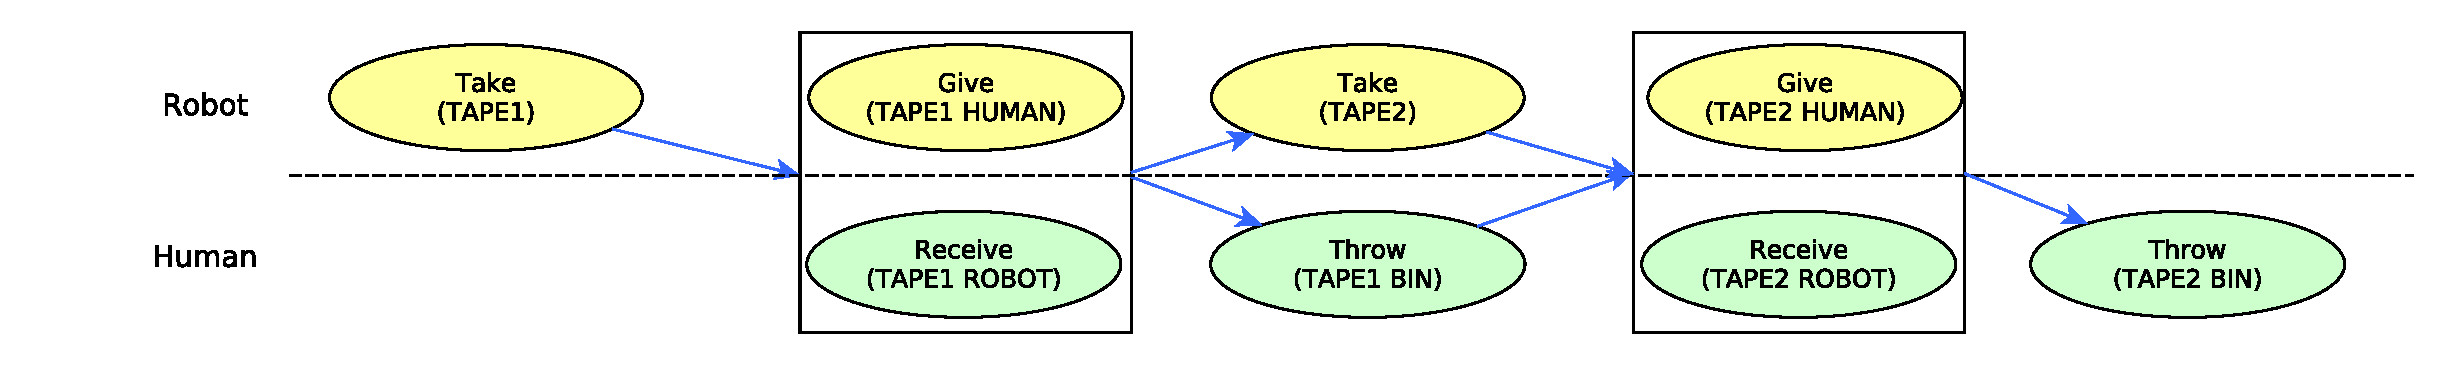
\includegraphics[scale=0.4]{img/coworker/results/plan2.pdf}
  }
  \label{fig:coworker_results_scenario2}
\end{figure}

While the robot is taking the \textit{TAPE1} the human moves
to take the \textit{TAPE2}. This deviates from the robot's plan, so it
switches to the \textit{equal partners} modality, communicating the change to\
the user. The user throws the \textit{TAPE2} in the \textit{BIN} while
the robot takes the \textit{TAPE1} and handles it to the user. The user
takes the \textit{TAPE1} and throws it in the \textit{BIN}, completing the task.

In the second run the current modality is \textit{human leader}. The user is
asked to clean the table as he wishes. The user asks the robot to take
each tape and give it to him, throwing them in the trashbin.

\item
\textbf{Replanning after failed action}. 
In this scenario (figure~\ref{fig:coworker_results-scenario3}) the robot is the only agent able to reach the
bin, while both agents can reach the two tapes. The
robot is in the \textit{robot leader} modality and, after examining the
environment, produces a plan.

\begin{figure}
  \caption[Robot coworker experiment 3]{Replanning after failed action. Here we can see a first
    plan, produced at the start of the scenario, and a second,
    produced after the robot fails to take the \textit{TAPE2}. }
  \centering
  \subfigure{
    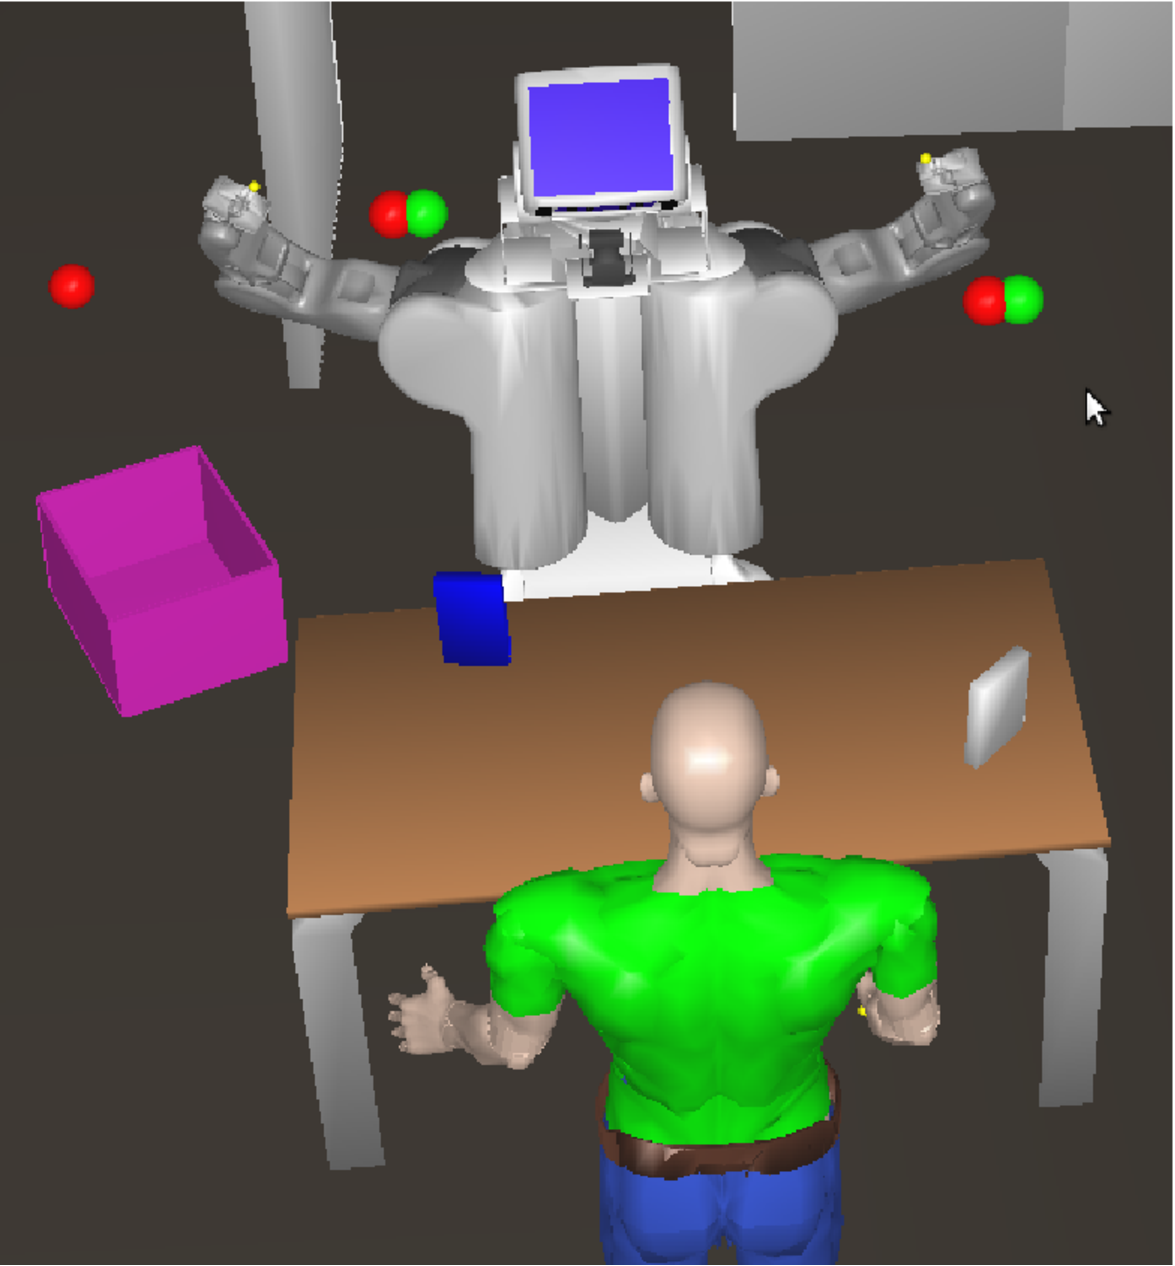
\includegraphics[scale=0.25]{img/coworker/results/scenario3.pdf}
    }
    \subfigure {
      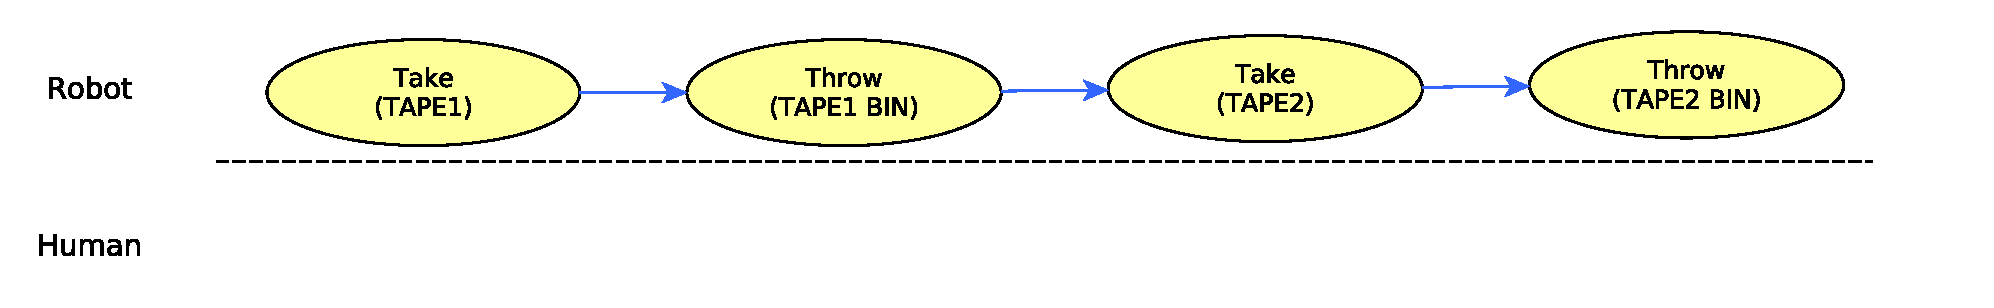
\includegraphics[scale=0.5]{img/coworker/results/plan3.pdf}

      }
      \subfigure {
        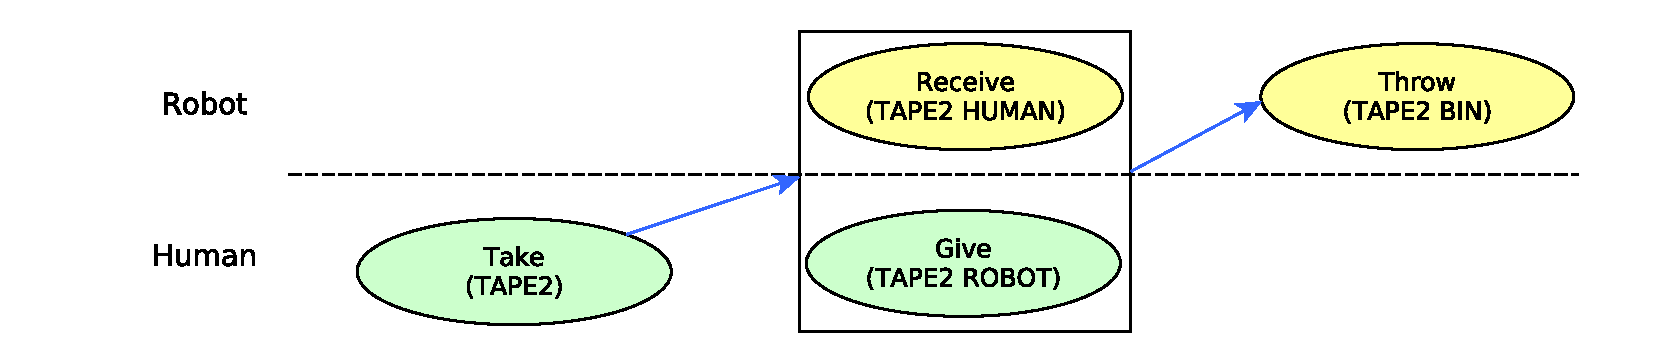
\includegraphics[scale=0.5]{img/coworker/results/plan4.pdf}
      }
  \label{fig:coworker_results-scenario3}
\end{figure}


After taking and throwing the \textit{TAPE1}, the robot tries to take the
\textit{TAPE2}, but fails because it is too far. The robot informs the user
and replans. The agents execute the plan, completing the task.

\item
\textbf{Replanning after human inactivity}.
In this run the robot computes that the \textit{TAPE3} and \textit{BIN}
are reachable only by the human, while the \textit{TAPE2} is reachable only by the robot. The robot computes a plan
and starts executing it, observing the human reactions. 
 After an initial stage when the human is
commited to the task, he does not execute a part of the plan (taking
the final tape and throwing it), so the robot looks for another
plan. The only solution to the problem is the one already computed at
the beginning, so the robot decides to ask
 the human to take the tape and throw it. A run of this
scenario is shown in figure ~\ref{fig:coworker_results-experiment}. 
\end{itemize}

 
\begin{figure}
  \caption[Robot coworker experiment 4]{The picture shows a run of our \textit{replanning after human
    inactivity scenario}. The different
    rows show, starting from top to bottom: the real world picture,
    the world state representation built by the robot, symbolic facts
    introduced in the knowledge base at each time step, action taken by the
    agents at each time step, the current plan calculated by the robot.}
  \centering
  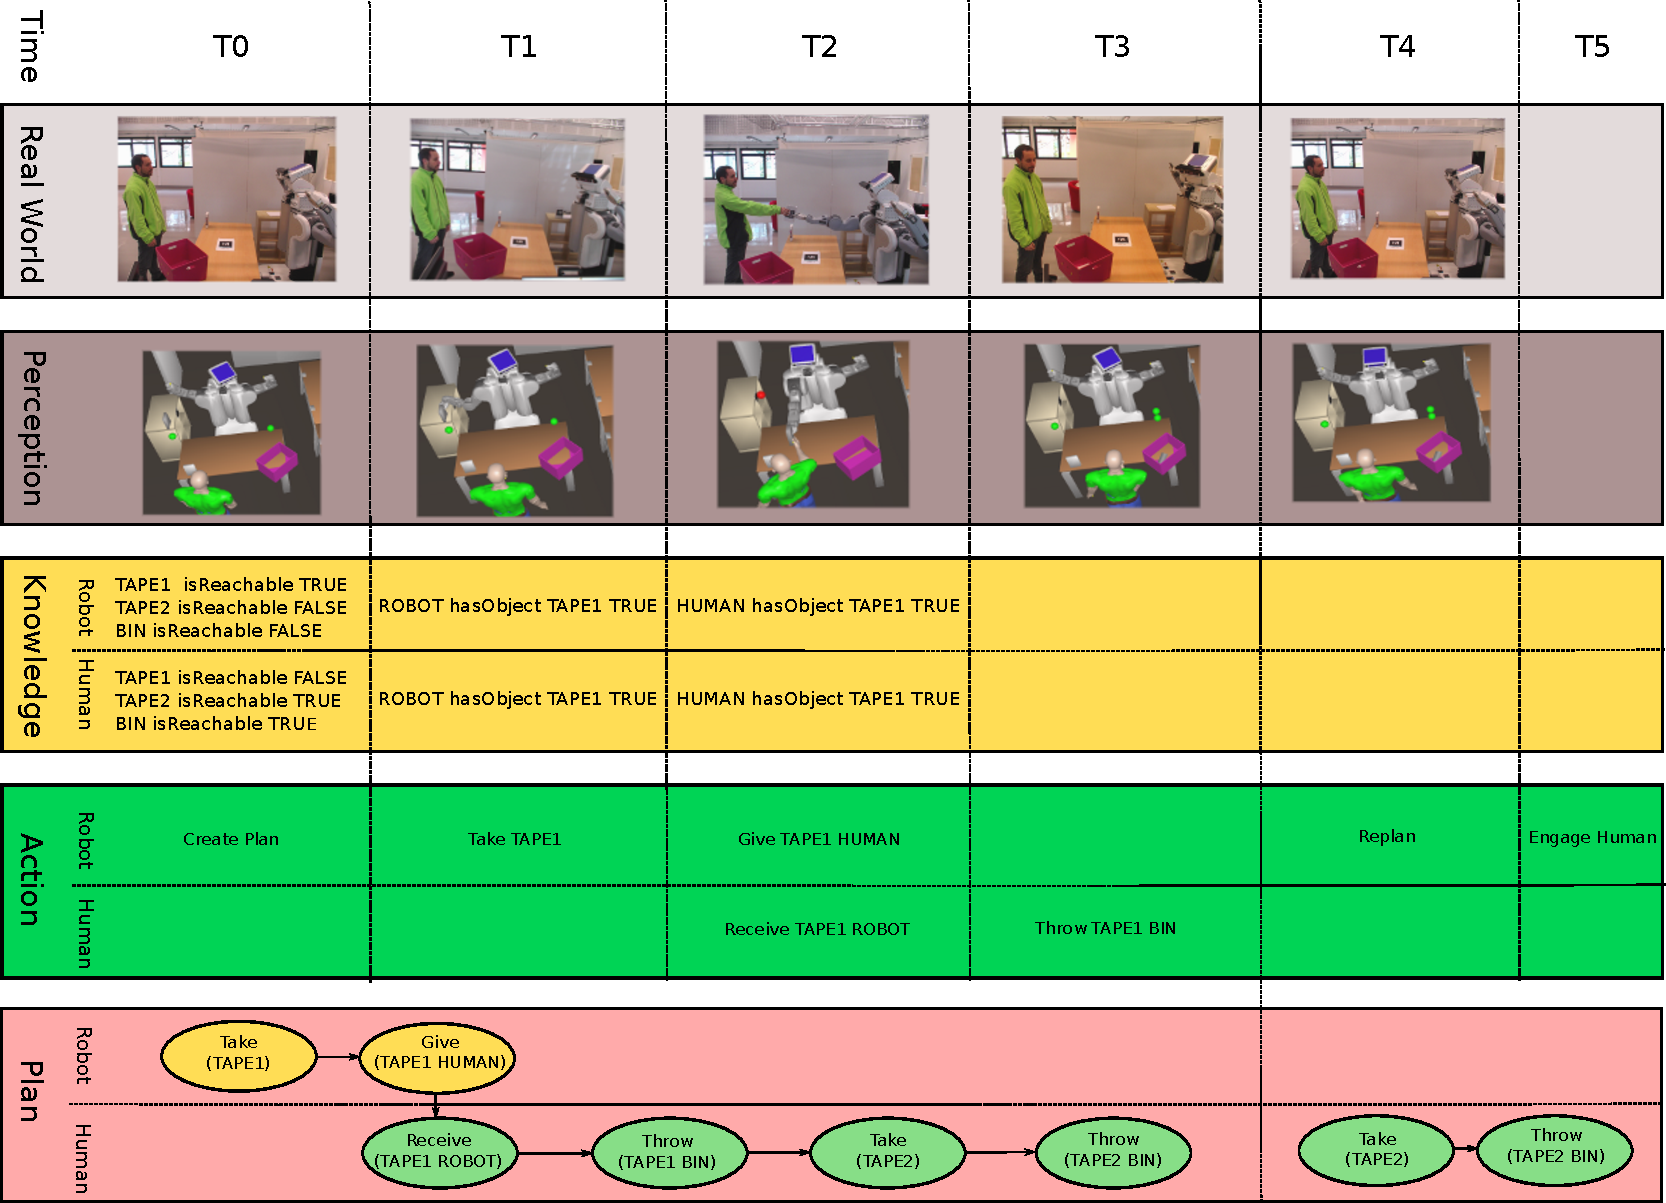
\includegraphics[angle=90, scale=0.7]{img/coworker/results/complete_plan.pdf}
  \label{fig:coworker_results-experiment}

\end {figure}


\section{Discussion}
\label{sec:coworker_experiments-discussion}
We review some of the main results of our experiments in this scenario:
\begin{itemize}

\item
\textbf{The system is able to handle joint goals}.
The system is able to create shared plans with different users, taking
into account the capabilities of each agent. When unexpected changes
in the world or task status arise, the system is able to quickly
replan, adapting to new scenarios. The system is able to execute this
joint goal in a human aware way. 
                                
\item
\textbf{The system is able to handle joint actions}.
The system is able to estimate user intentions in collaborative tasks and to choose appropriate actions, using a set of MOMDP models.

\item
\textbf{The system is able to handle user preferences}.
The system is able to adapt itself to user preferences, allowing the
human partner to give commands or to be more passive in its role and
switching from one modality to the other. 
\item
\textbf{The system is able to handle each agent beliefs}.
The system is able to represent different belief states for different agents and to take into accout what users can see, reach and know when creating a plan.

\item
\textbf{The system is able to monitor human actions}.
The system was able to understand when the human performed action such as taking or throwing objects.
\end{itemize}

 
\chapter{Human-Aware Probabilistic Planning}
\label{chapter:mamdp}

\lhead{Chapter 9. \emph{Human-Aware Probabilistic Planning}} % Change X to a consecutive number; this is for the header on each page - perhaps a shortened title

In this section we present a recent work where we developed a Multi-Agent Markov Decision Process (MAMDP). Section~\ref{sec:mamdp-intro} presents the problem. Section~\ref{sec:mamdp-overview} briefly introduces our approach, which is explained fully in section~\ref{sec:mamdp-single_agent} and section~\ref{sec:mamdp-mamdp}. Section~\ref{sec:mamdp-discussion} discusses the characteristics of this model, while section~\ref{sec:mamdp-example} show an example of creation of a MAMDP, starting from single-agent models. Finally, section~\ref{sec:mamdp-plan_monitoring} proposes an extension to the plan monitoring algorithm previously introduced, that would allow our system to monitor tasks and evaluate human engagement in collaborative activities.


\section{Introduction}
\label{sec:mamdp-intro}
Multi-Agent planning   is an important and studied topic in the AI community \citep{durfee1999survey}. There are several approaches to this problem, using classical or probabilistic planning. There are several issues to consider:
\begin{itemize}
\item Distributed vs Centralized. A multi-agent planner might be distributed, meaning that separate systems plan independently and then communicate to build a shared plan (an idea investigated, for example in \cite{nikolaidis2013cross,guestrin2002distributed} ); or centralized, meaning that a single system plans for all the agents.
\item Coordination. Agents need to coordinate their plans, in particular in the presence of shared resources. Imagine, for example, two agents, Max and Bob, that are using a tool to repair a set of cars. If Max is proceeding faster than Bob and the two do not coordinate, Max might take the tool and leave, starting to repair another car, ignoring the fact that Bob still needs the tool. This example shows that it is important to reason on the duration of actions performed by agents. At the simplest level, agents need to know the advancement of the sub-plan of other agents. More complex reasoning might take into account how long an agent needs to perform a certain sub-task, in order to refine a plan. 
\item Cooperation. Even when performing different sub-tasks of the same plan, agents can help each other, for example by passing items, thus improving the efficiency of the plan. Multi-Agent problems can be loosely or tightly coupled, depending on the quantity of interactions between agents. Some works are not focused specifically on tightly or loosely coupled problems, and try to present a generic approach. \cite{torreno2015approach} proposes a cooperative refinement planning approach, based on the partial-order planning paradigm. In this work each agent refines a centralized plan. Agents are able to exchange information, since the complete world-state might not be observable by everyone. Refined plans are then analyzed by each agent, and voted with a democratic leadership approach. Results show that this approach is very efficient at solving loosely coupled problems, but also competent on tightly coupled situations. 

\item Communication and Knowledge. In a multi-agent environment each agent might have an incomplete or incorrect belief on the world, which might lead to wrong or sub-optimal actions. Agents may communicate to progressively build a correct belief model on the world state. 
\end{itemize}

Several approaches has been studied to bring the multi-agent planning problem in a probabilistic framework. \cite{boutilier1999sequential} create a centralized MDP, able to select at each time step actions for every present agent. Dec-POMDP \citep{bernstein2002complexity} and I-POMDP \citep{gmytrasiewicz2005framework} are more complex frameworks, that take into account the belief models of agents. The complexity of these models makes them difficult to use in even moderately difficult scenarios. A solution to this problem is considering simpler problems, where the agents mostly work independently and interact only in limited situations, such as in \cite{melo2013heuristic}.  Since we are more interested in tightly coupled scenarios, where the robot and human interact often, these kind of approaches are not suitable.

\section{Overview}
\label{sec:mamdp-overview}
In some situations, the environment, or other agents' actions, can be very unpredictable, and the system needs to constantly adapt its plans to the current state of the world, by replanning or repairing processes, which can be expensive. To deal with this issue we developed a Human-Aware Probabilistic Planner, based on MDPs. Our goal is replicating the characteristics of HATP, which we presented in section~\ref{sec:plan_management-hatp}, in a probabilistic domain. We designed this planner with the following ideas:

\begin{itemize}
\item Centralization. We will use a single planner, which chooses actions for all the involved agents.
\item Hierarchical. The domain will be split in different modules, which interact to achieve the goal. Hierarchical models allow us to speed up the computation of the MDP policy and to reuse models in different domains and tasks.
\item Tightly Coupled. We will focus on problems where the agents' interactions are frequent.
\item No Communication. The planner will  assume that all the agents have perfect knowledge of the world state. The rest of the system will have to take care of maintaining users' knowledge, ensuring the correct execution of the plan. Current planners that try to include communication issues often focus on loosely coupled interactions between the agents, in order to simplify the domain and be able to compute a policy for the problem. Since we choose to focus on tightly coupled problems, we can not use this solution, and so prefer to avoid the issue at this level.
\end{itemize}

This work is a very recent development, and has not yet been integrated in the rest of the system. We will explain the main characteristics of the MAMDP in the following sections.


\section{Single-Agent MDP}
\label{sec:mamdp-single_agent}
The starting point for this planner is the single agent MDP. We start with the classical model \\ $(S,A,T,C,G,S_0)$, where $S$ is the system space, $A$ is the set of actions, $T(s_i,a,s_j)$ is the probability to transition from state $s_i$ to state $s_j$ after taking action $a$, $C(s,a)$ is the cost of taking action $a$ in state $s$, $G \in S$ is the set of goal states, and $S_0 \in S$ is the set of starting states. We express the state space $S$ of the system as a set of variables $var$, each one with a possible range of values $values(v)$, where $v$ is a variable.

 We develop this model in the following way.

\subsection{Parameters}
We can define parameters in our MDP, and assign them to different values. We will call the list of parameters of a MDP $par$ and their current instantiation the \textit{parameter\_instance} of the model. Parameters can be linked to variables and values. We call $par\_var$ the variables associated to a parameter. 

For example, let us imagine a scenario of a room, with different furniture and objects. Let us define the state space of a generic MDP to take an object in this room. We can define two variables: the location of an agent, \textit{agent\_isAt}, which can assume values in the set ${f_1, f_2, f_3}$ (where $f_i$ represent a furniture in the room); and an object variable, \textit{object\_isAt}, which can assume the same values as the \textit{agent\_isAt} variable. If we define two parameters, \textit{agent} and \textit{object}, and link them to the \textit{agent\_isAt} and \textit{object\_isAt} variables, we can create a generic MDP which can be used to plan for any agent (with similar capacities) to take an object in this room.

The MDP receives as input, when consulted to select an action, the state of the world,  which we will call \textit{real\_space}. The \textit{real\_space} will be converted, using the \textit{parameter\_instance}, to the \textit{parameter\_space}, which will be actually used by the model in its computations. 

For example, in the real world, we have two agents, \textit{Bob} and \textit{Greg}, and three objects \textit{glue}, \textit{book}, \textit{smartphone}. If we assign the \textit{agent} parameter to \textit{Bob} and the \textit{object} parameter to \textit{book}, when receiving the complete world state the MDP will assign as \textit{agent\_isAt} the location of Bob, and as \textit{object\_isAt} the location of the book, discarding unneeded variables.

Parameters allow us to create smaller, generic MDPs, which can be reused easily.


\subsection{Actions and Macro Actions}
We define actions as a tuple $(subject,action\_name,object,target)$, where each element of the tuple is called an $action\_part$.  We represent the action as a string, composed by its $action\_parts$, joined by the character `\_' as delimiter. For example, an action where Greg places a book on a table can be represented as \textit{Greg\_place\_book\_table}. We define the function $convertPar(a)$ and $convertReal(a)$ to convert action $a$ to the \textit{real\_space} or the \textit{parametrized\_space}.

We add to the normal set of actions of a MDP \textit{macro actions}, linked to other MDPs, which allow us to create a hierarchy of MDPs. We call $M$ the set of \textit{macro actions} of the MDP, and $sub(a)$ the sub-MDP linked to the \textit{macro action} $a$. For example, we might create, in a MDP whose goal is cleaning a room, a macro action to reorder the room's objects and one to clean the floor. Each of these macro actions will be linked to a specific MDP, who will refine the problem in more details.

The cost of executing a macro is directly computed from the sub-MDP. There are several strategies to compute this cost, like in \cite{dietterich2000hierarchical,hauskrecht1998hierarchical}.

\subsection{Name and Parameter Name}
We define for each MDP model a \textit{name}, which identifies it, and a \textit{parametrized\_name}, which substitutes parameters using the \textit{parameter\_instance}. The \textit{name} is defined using the same tuple as an action. 

For example, a MDP whose goal is to obtain an object could have as \textit{name} $agent\_get\_object$ and as \textit{parametrized\_name}, in a certain moment, $Greg\_get\_book$.

We define a function $assignParameterFromActionName(a)$ which creates the \textit{parameter\_instance} of the MDP based on an action name. This function can be very useful when using \textit{macro actions}, so that the system can assign parameters to the sub-MDP from the \textit{macro action} string and then consult it.

For example, if the \textit{macro action} $Greg\_get\_book$ is linked to the $agent\_get\_object$ MDP, this function would assign values to the  $agent\_get\_object$ model's parameter. The system would assign the value $Greg$ to the $agent$ parameter and the value $book$ to the $object$ parameter. 

Each \textit{name} can be divided in a number of $name\_parts$,  with the same procedure as actions. The \textit{parametrized\_name} can be divided as well in $parametrized\_parts$.


\subsection{Abstract States}

In some situations, a model might not need to base its planning choices on all the possible values of a variable in the \textit{real\_space}. Imagine, for example, the case where an agent needs to perform a series of operations on the furniture $f_1$ in the room. In this case, we could model the  values of the \textit{agent\_isAt} variable as $\{f_1 , other\_location\}$, greatly reducing the state space. In this situation we say that \textit{agent\_isAt} is an \textit{abstract variable}. 

We build a map $abstract\_values_v$ for each abstract variable $v$, which links real world values to model values (e.g. $f_2 \rightarrow other\_location$). This map will be used to convert a state expressed in the $real\_space$ to the $parameter\_space$ of the model. 
%The choice of using abstract variables needs to be carefully weighted, because they can impact on the quality of the solution of the model.

\section{Multi-Agent MDP}
\label{sec:mamdp-mamdp}
Now we will explain how we build a Multi-Agent MDP (MAMDP), starting from $n$ single-agent models, one for each agent. We will call the single-agent models $MDP_i$, where $1 \leq i \leq n $ is the index of the agent. In the following paragraphs, we will use the notion $S_i, var_i, values_i, A_i, T_i, C_i, G_i, S_{0i}, M_i, par_i, par\_var_i$ when referring to components of the single-agent MDP, adding the $i$ index to differentiate them from the MAMDP. 
 
\subsection{Name and Parameter Name}
The \textit{name} and \textit{parameter\_name} of the MAMDP are built by concatenating those of its agent MDPs, adding the `-' character to separate the single agents.

For example, the \textit{name} of a MAMDP with single-agent models \textit{agent\_get\_object} and  \textit{agent\_clean\_table} is \textit{agent\_get\_object-agent\_clean\_table}.

\subsection{State Space and Parameters}
$par=\bigcup_{1 \leq i \leq n, p \in par_i} p+\text{`p'}+i $ \\
$par\_var=\bigcup_{1 \leq i \leq n, v \in par\_var_i} \> rename(v)$ \\
$var=\bigcup_{i=1}^{n}(var_i \setminus par\_var_i) \cup par\_var$ \\
$\forall_{v \in var}\> values(v)=\bigcup_{i| v \in var_i} 
\begin{cases}
	 values_i(v) \quad \text{if } v \not \in par_i \\
	 p+\text{`p'}+i \quad \text{if } v \in par_i \\
\end{cases}$ \\ 

To create the set of parameters of the MAMDP we will rename each parameter in the single-agent MDPs, adding an identifier composed by `p' and by the index of the MDP. We make this choice because different MDPs could share the same parameters, but they could be assigned to different values, and so need to be treated as separate entities, even if they have the same semantic meaning. Parameter variables are created by renaming the parameter variables of the sub-MDPs to account for this newly added identifier.

For example, if the $MDP_1$ model has a parameter \textit{object}, linked to a variable called \textit{object\_isAt}, we will rename the parameter as \textit{objectp1} and the variable as \textit{objectp1\_isAt}. 

We defined $S$ as the union of the variables of the single-agent MDPs excluding their parameter variables. We will instead take the parameter variables of the MAMDP, in the way that we just defined.

The MAMDP variable can assume all the possible values that are available in the corresponding variables of the sub-MDPs. As before, we will change values that are parameters to account for our renaming procedure. 

We define the function $single_i(s)$ , which converts the MAMDP state to state of the single-agent MDP $i$.


\subsection{Actions}
$A=(\prod_{i=1}^{n} A_i) \cup JointActions \cup WaitActions$ , where $JointActions$ is the set of collaborative actions, and $WaitActions$ is a set computed by enumerating all the possible instances where one or more agents do not act, and simply wait, while others are acting.

The actions of the MAMDP are a concatenation of the actions of the single MDP, adding the separator character `-' between the different agents' actions. We will refer to the single agent's actions of action $a$ as $a_i \quad \forall \> 1\leq i \leq n$.

For example, the MAMDP will contain actions such as `agentp1\_move\_surface1-agentp2\_move\_surface2'.

We add to $A$ the special set of $JointActions$, which are actions that the agents can use to cooperate. For example, if there is a resource in a single agent MDP which two agents can possess, we introduce a $handover$ action between them. 

For each $a \in A$, if there is a sub-action $a_i$ which is a macro action for MDP $i$, we create a new MAMDP and assign it as sub-MAMDP of $a$. This sub-MAMDP will be created from $n$ MDP models, as for its father, in the following way. Let $f$ be the father MAMDP, $c$ the sub-MAMDP, and $a$ the macro-action of $f$. \\
 $ \forall_{\text{MDP}\> m_i \in f}$ we assign a MDP $m_j$ in $c$ where:\\
$m_j= \begin{cases}
	m_i & \quad \text{if } a_i \not\in M_i \\
	sub_i(a_i) & \quad \text{if } a_i \in M_i 
\end{cases}$ \\

\subsection{Transition Function}
\label{subsec:mamdp-transition}
$T(s_a,a,s_b)=
\begin{cases}
\prod_{i=1}^{n}(T_i(single_i(s_a),a_i,single_i(s_b))) & \> \text{if } !isIncongruent(s_a)\; \land  \;!isIncongruent(s_b)  \\
0   & \quad \text{else}
	\end{cases}$ \\

The transition function is computed as the product of the transition functions of the single agent MDPs, on the converted states and actions.

We set the probability as zero if either the starting or ending states state of the transition are incongruent. This is done by converting the states to the \textit{real\_space} and checking the values of the different variables. We say that a state is incongruent if two non abstract variables in the \textit{parameter\_space}, that are assigned to the same \textit{real\_space} variable, have different values. If one or both the variables are abstract we check if their $abstract\_values$, for the current variable values, have a value in common. If not, we consider the state incongruent.

For example, consider the state $(objectp1\_isAt=`surface', objectp2\_isAt=`table', agentp1\_isAt=`table', agentp2\_isAt=`table')$. If in the current \textit{parameter\_instance} both \textit{objectp1} and \textit{objectp2} are assigned to the same variable, this state will be incongruent.

Consider now the state $(objectp1\_isAt=`agentp1', objectp2\_isAt=`other', agentp1\_isAt=`table', \\ agentp2\_isAt=`table')$. If $objectp1$ is a parameter assigned to $Greg$, \textit{objectp1\_isAt} is an abstract variable, and $abstract\_values_{objectp2\_isAt}(`Greg')=`other'$, this state will not be considered incongruent.  

%CORRECTION MOUADDIB
While building the MAMDP, we assume that the transition functions of the single agents are independent. For example, we are not able to model the possibility that an agent is more likely to fail an action that requires his concentration if another agent is moving around the area disturbing him.
%END_CORRECTION MOUADDIB

\subsection{Start and Goal States}
$S_0=s \in S\; | \; \forall_{i=1}^n s_i \in S_{0i} $. A state is a starting state in the MAMDP only if it is a starting state in all the single agent MDPs.\\
$G=s \in S\; | \; \exists_{i=1}^n \; | \; s_i \in G_{i}$. A state is a goal state in the MAMDP if it is a goal state in any one of the single agent goal states. The idea of this choice is that a MAMDP terminates when one of the agents has achieved its goal. If there is an agent that has not completed its task, and the MAMDP was a sub-model in a hierarchy, its father will select another action, perhaps assigning one or more agents to the uncompleted task. 

In some situations, we might try creating a MAMDP composed of opposing goals, like for example, a MAMDP where both agents need to get the same object. Since we are interested in cooperative and not competitive scenarios, we will not create these kind MAMDPs. We can recognize this situation by checking if there is any state in $G$ that is incongruent, as previously defined in subsection~\ref{subsec:mamdp-transition}. 


\subsection{Cost Function}
$C(s_a,a,s_b)= 
	\begin{cases}
		max_{i=1}^{n}(C_i(single_i(s_a),a_i,single_i(s_b))  & \quad \text{if } s_b \not\in G \\
		\sum_{i | single_i(s_a) \not\in G_i} expectedCost_i(single_i(s_a))  & \quad \text{if } s_b \in  G
		\\
	\end{cases} $	\\

where $expectedCost_i(s)$ is a function that computes the expected cost for agent $i$ to reach a goal state by starting in state $s$ and following the action policy. In this calculation, we allow from the other agent only $JointActions$ that are necessary to solve the plan (e.g. handovers if the agent does not have a needed resource).

The cost function of the MAMDP is chosen by taking the maximum cost of the single agent actions that are executed, if the state $s_b$ is not a goal state. If it is a goal state, we take as cost an estimation of the time required by any agent that has not reached his goal to complete their tasks, with only minimal cooperation. In this way, we encourage the MAMDP to choose plans where the agents cooperate and do not only try to achieve their goal.

\section{Discussion}
\label{sec:mamdp-discussion}

The result of this fusion is a MDP, that can be solved with well-known algorithms, like value iteration. By fusing all the possible MDPs, the resulting model can be  very hard to solve but, using macro actions, parameters, and abstract states we can greatly reduce its complexity. 

The action space of the joint model is calculated as the cross product of the action spaces of the single model. When there are several macro actions in the agent models, this could result in the creation and computation of the policy of several sub-models, which can significantly slow down the computation of a solution for the model. We can reduce the complexity of this process by making several considerations.

First of all, created MAMDPs can be reused in different branches of the hierarchy, if needed. When creating a new MAMDP, we will look to see if there is already an existing MAMDP with the same $name$ and, if so, we will use it.

Second, parameters can greatly  reduce the number of sub-MAMDPs to compute. Let $a$ be a \textit{macro action}, $c$ the sub-MAMDP linked to $a$, $1..n$ the indexes of the single-agent MDPs of $c$, which are selected as previously explained.

 We create the \textit{parametrized\_name} of $c$ by concatenating the \textit{parametrized\_name} of its single-agent MDPs. To set the $name$ of  $c$ we process each name of its single-agent MDPs $name_i$, by modifying all of its $name\_parts_{i,k}$, with $1 \leq k \leq m$ in the following way:\\
$name\_part_{i,k}=
\begin{cases}
	name\_part_{i,k} & \quad \text{if } !parametersInCommon(name\_part_{i,k}) \\
	parametrized\_part_{i,k} & \quad \text{else}
\end{cases}$ \\
where $parametersInCommon(name\_part_{i,k})$ is a function that returns true if $name\_part_{i,k}$ is a parameter in sub-MDP $i$, and there is a sub-MDP with index $j$, where $name\_part_{i,k}$ is a parameter or variable. \\

The idea behind this choice is the following. If the sub-MDPs do not have parameters in common, we can use a generic MAMDP to represent this instance. For example, if we create a MAMDP for the macro action $agent1\_clean\_table-agent2\_clean\_shelf$, we can use the MAMDP $agent\_clean\_furniture-agent\_clean\_furniture$ since the sub-MDP models do not have parameters in common, and their actions will not conflict.

 If instead we create a MAMDP for the macro action $agent1\_clean\_table-agent2\_clean\_table$ we create a specialized MAMDP, since there are parameters in common ($table$) and if we treat them as different objects there could be incongruences in the MAMDP planning.



\section{Example}
\label{sec:mamdp-example}
In this section we will show an example of creation of a MAMDP. We start by presenting a cooperative scenario. The robot and a human are working together to assemble three brackets on three different work surfaces. To assemble a bracket the agents need to clean the surface, apply some glue to it, and fix the bracket. A possible set-up for this scenario is shown in figure ~\ref{fig:mamdp-mamdp_scenario}.

 \begin{figure}[ht!]
	\centering
	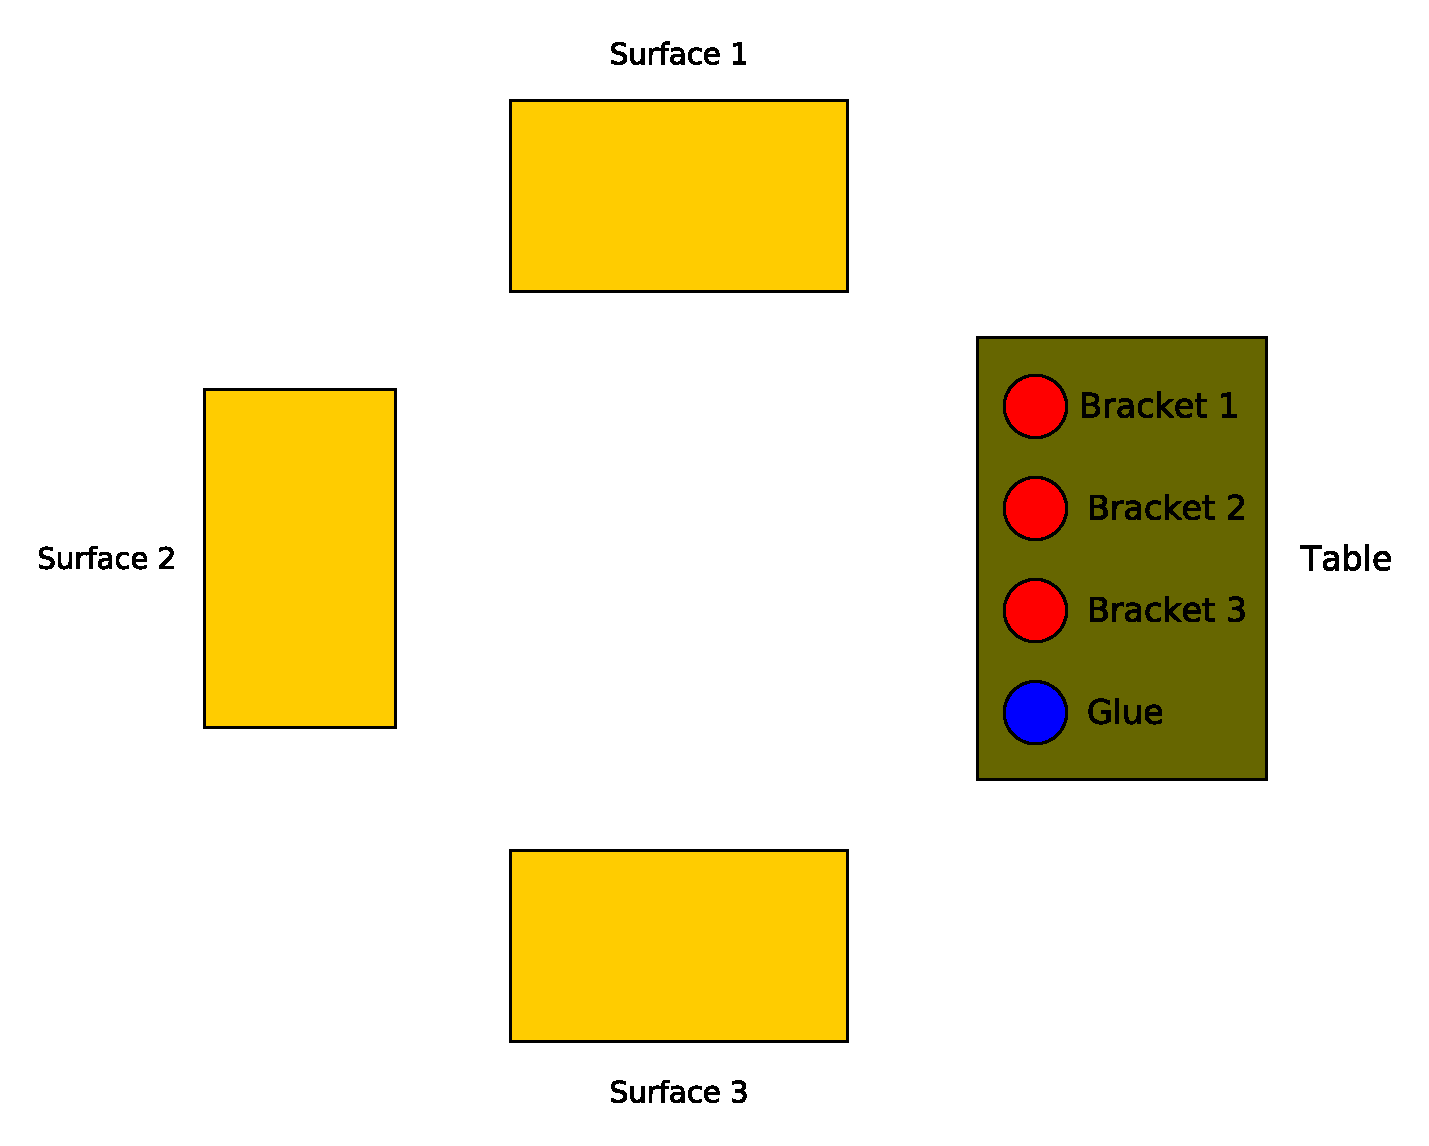
\includegraphics[scale=0.5]{img/coworker/mamdp/scenario.pdf}
	\caption[MAMDP example: scenario]{The image shows the set-up for this example scenario. The four locations are represented as different rectangles and the objects as circles. }
	\label{fig:mamdp-mamdp_scenario}
\end{figure}

\subsection{Single-Agent MDP}

We start by defining a single-agent MDP for this scenario. We will use a hierarchical architecture, as shown in figure~\ref{fig:mamdp-scenario_single_architecture}. This architecture is composed by three different modules: AssembleAllBrackets, which controls the flow of the scenario; AssembleBracketSurface, which assembles a chosen bracket on a chosen surface; and GetObject, which obtains an object. We will create some simplifications in these models, as they are chosen just to explain how we build a MAMDP, and not for a realistic use.

\begin{figure}[ht!]
	\centering
	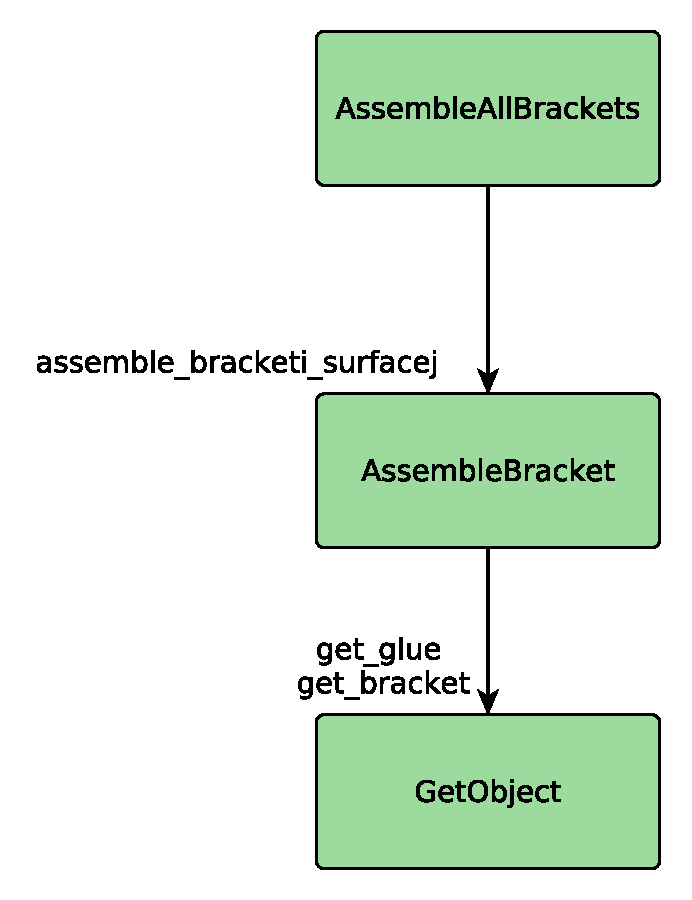
\includegraphics[scale=0.5]{img/coworker/mamdp/scenario_single_architecture.pdf}
	\caption[MAMDP example: single MDP model]{The image shows the architecture for the single agent MDP of the MAMDP example scenario. The various MDPs are represented as rectangles. The arrows show the links between hierarchical modules in the architecture. The label of the arrow shows the macro action corresponding to the link. The label \textit{assemble\_bracketi\_surfacej} actually correspond to all the combinations to assemble a bracket on a surface. We grouped them since, as the AssembleBracketSurface MDP uses parameters, it can be used for all these macros.}
	\label{fig:mamdp-scenario_single_architecture}
\end{figure}



\subsubsection{AssembleAllBrackets}
We will now show the \textit{AssembleAllBrackets} model, whose goal is directing the flow of the scenario, by choosing which bracket should be assembled on which surface.

\begin{itemize}
	\item $name: agent\_assembleallbrackets$.
	\item		$par: agent$.
		\begin{itemize}
			\item $par\_var(agent)=agent\_isAt$.
		\end{itemize}
		In this example, we decided to create generic models which can plan either for Greg or for the robot.
	\item $S:\;\{agent\_isAt,bracket1\_isAt,bracket2\_isAt,bracket3\_isAt,surface1\_status,\\ surface2\_status,surface3\_status\}$. 
		\begin{itemize}
			\item $values(agent\_isAt):\{table,surface1,surface2,surface3\}$.
			\item $values(bracketi\_isAt):\{table,surface1,surface2,surface3,agent,other\_agent\} \forall_{i=1}^3$. 
			\item $values(surfacei\_status):\{completed,other\_status\}\;\forall_{i=1}^3$.
		\end{itemize}
		\begin{itemize}
			\item $abstract\_values\_surfacei\_status:$ 
				\begin{itemize}
					\item $none: other\_status$.
					\item $cleaned: other\_status$.
					\item $glued: other\_status$.
				\end{itemize}
			\item $abstract\_values\_bracketi\_isAt$ 
				\begin{itemize}
					\item $greg: other\_agent$.
					\item $robot: other\_agent$.
				\end{itemize}	
		\end{itemize}
		The state set of the model contains the location of the agent, of the brackets, and the status of the surfaces. The agent and the objects can be located at the table or at one of the surfaces. In addition, objects can be possessed by another agent. The status of a surface can be set to none, meaning that the fixing process as not started; cleaned, meaning that the agent has already cleaned the surface; glued, meaning that the agent has applied glue to the surface; and completed, meaning the a bracket ha been fixed on it. 

		To simplify the model we consider the states $none,cleaned,glued$ as abstract states. We also consider $other\_agent$ as an abstract value, assigned to both agents present in the scenario. Let us consider, for example, that the instance of the \textit{agent} parameter is \textit{greg}, and that in the \textit{real\_space} \textit{bracket1\_isAt=greg}. It could seem that, when converting from \textit{real\_space} to \textit{parameter\_space}, the system would assign \textit{bracket1\_isAt} to \textit{other\_agent}, since \textit{other\_agent} is an abstract value for \textit{greg}. In reality, the system will give priority to the current parameter, and execute the conversion properly, by setting \textit{bracket1\_isAt=agent}. 
	\item $A:\;\{agent\_assemble\_bracketi\_surfacej\}\;\forall_{i=1}^1 \forall_{j=1}^3$.
	\item $M: A$.

	All of this model's actions are actually \textit{macros}.
	\item $G:\; \cup_{s:S}\; |\; \forall_{i=1}^3\; surfacei\_status=completed\;\text{AND}\;\\
	forall_{i=1}^3\;\exists_{j}\;|\;bracketi\_isAt=surfacej\; \text{AND} \\
	\forall_{i,j=1}^3\; bracketi\_isAt \neq bracketj\_isAt.$

	The goal of this model is to fix all the brackets on the surfaces. We set as goal states every state in which the brackets are located on different surfaces and the status of each surface is \textit{completed}. 
	\item $S_0:\; \cup_{s:S}\;|\; \exists{1\leq i \leq 3}\; |\; surfacei\_status \neq completed$.

\end{itemize}

Note that we did not need to specify a cost function for this model. Since all of its actions are \textit{macros}, the cost function will be directly derived from its sub-models.

\subsubsection{AssembleBracket}
We will now show the \textit{AssembleBracket} model, whose goal is assembling a specific bracket on a specific surface.
\begin{itemize}
	\item $name: agent\_assemble\_bracket\_surface$.
	\item		$par: \{agent,bracket,surface\}$.
		\begin{itemize}
			\item $par\_var(agent)=agent\_isAt$.
			\item $par\_var(bracket)=bracket\_isAt$.
			\item $par\_var(surface)=surface\_status$.
		\end{itemize}

	\item $S:\;\{agent\_isAt,bracket\_isAt,surface\_status,glue\_isAt\}$. 
		\begin{itemize}
			\item $values(agent\_isAt):\{surface,other\_location\}$.
			\item $values(bracket\_isAt):\{agent,surface, other\_location,other\_agent\}$. 
			\item $values(glue\_isAt):\{agent,other\_location,other\_agent\}$. 
			\item $values(surface\_status):\{none,cleaned,glued,completed\}$.
		\end{itemize}
		\begin{itemize}
			\item $abstract\_values\_bracket\_isAt$: 
				\begin{itemize}
					\item $surfacei=other\_location\; \forall_{i=1}^n$ .
					\item $table=other\_location$.
					\item $greg=other\_agent$.
					\item $robot=other\_agent$.
				\end{itemize}	
			\item $abstract\_values\_glue\_isAt=abstract\_value\_bracket\_isAt$ 
			\item $abstract\_values\_agent\_isAt$:
				\begin{itemize}
					\item $surfacei=other\_location\; \forall_{i=1}^n$ .
					\item $table=other\_location$.
				\end{itemize}
		\end{itemize}
		
		This state set will contain, other than the variables of \textit{AssembleAllBrackets}, also the location of the glue bottle. In this situation, \textit{surface\_status} will not be an abstract variable, since the model needs to know what is the exact state of the fixing process. We greatly simplified the number of locations where agents and objects can be present by using abstract variables. This model is only interested in knowing if the agent has an object (glue or bracket) or not. In the case where the agent does not have an object, it can invoke the \textit{get\_object macro}, which will take charge of obtaining it, using a more complete state space.
	\item $A:\;\{agent\_move\_surface,agent\_clean\_surface,agent\_glue\_surface,\\
	agent\_fix\_bracket,agent\_get\_bracket,agent\_get\_glue\}$.
	\item $M:\;\{agent\_get\_bracket,agent\_get\_glue\}$.
	\item $G:\; \cup_{s:S}\; |\; surface\_status=completed$.
	\item $S_0:\; \cup_{s:S}\; |\; surface\_status \neq completed$.
\end{itemize}


\subsubsection{GetObject}
We will now show the \textit{GetObject} model, whose goal is obtaining an object in the environment.

\begin{itemize}
	\item $name: agent\_get\_object$.
	\item		$par: \{agent,object\}$.
		\begin{itemize}
			\item $par\_var(agent)=agent\_isAt$.
			\item $par\_var(object)=object\_isAt$.
		\end{itemize}

	\item $S:\;\{agent\_isAt,object\_isAt\}$. 
		\begin{itemize}
			\item $values(agent\_isAt):\{table,surface1,surface2,surface3\}$.
			\item $values(object\_isAt):\{table,surface1,surface2,surface3,agent,other\_agent\}$. 
		\end{itemize}
		\begin{itemize}
			\item $abstract\_values\_object\_isAt$:
				\begin{itemize}
					\item $greg=other\_agent$.
					\item $robot=other\_agent$.
				\end{itemize}	
		\end{itemize}
		The state set of this model contains a more detailed representation of the possible locations of the scenario, since the goal of the agent is obtaining an object.		

	\item $A:\;\{agent\_move\_table, agent\_move\_surface1\, agent\_move\_surface2, \\ 
	agent\_move\_surface3, agent\_take\_object\}$.
	\item $M:\;{\emptyset}$.
	\item $G:\; \cup_{s:S} \; | \; object\_isAt=agent$
	\item $S_0:\; \cup_{s:S} \; | \; object\_isAt \neq agent$
\end{itemize}

\subsection{MAMDP}
We will now show how our MAMDP is created. The MAMDP hierarchy, shown in figure~\ref{fig:mamdp-scenario_mamdp_architecture} will contain different models. At the highest level lies the model \textit{AssembleAllBrackets-AssembleAllBrackets}, a duplication for two agents of the highest module in the single agent MDP hierarchy. The lowest modules include different combinations of the single agent sub-MDPs, in order to account for the possible task allocations. We will start by showing the top MAMDP model.

\afterpage{\clearpage}
\begin{sidewaysfigure}[ht!]
	\centering
	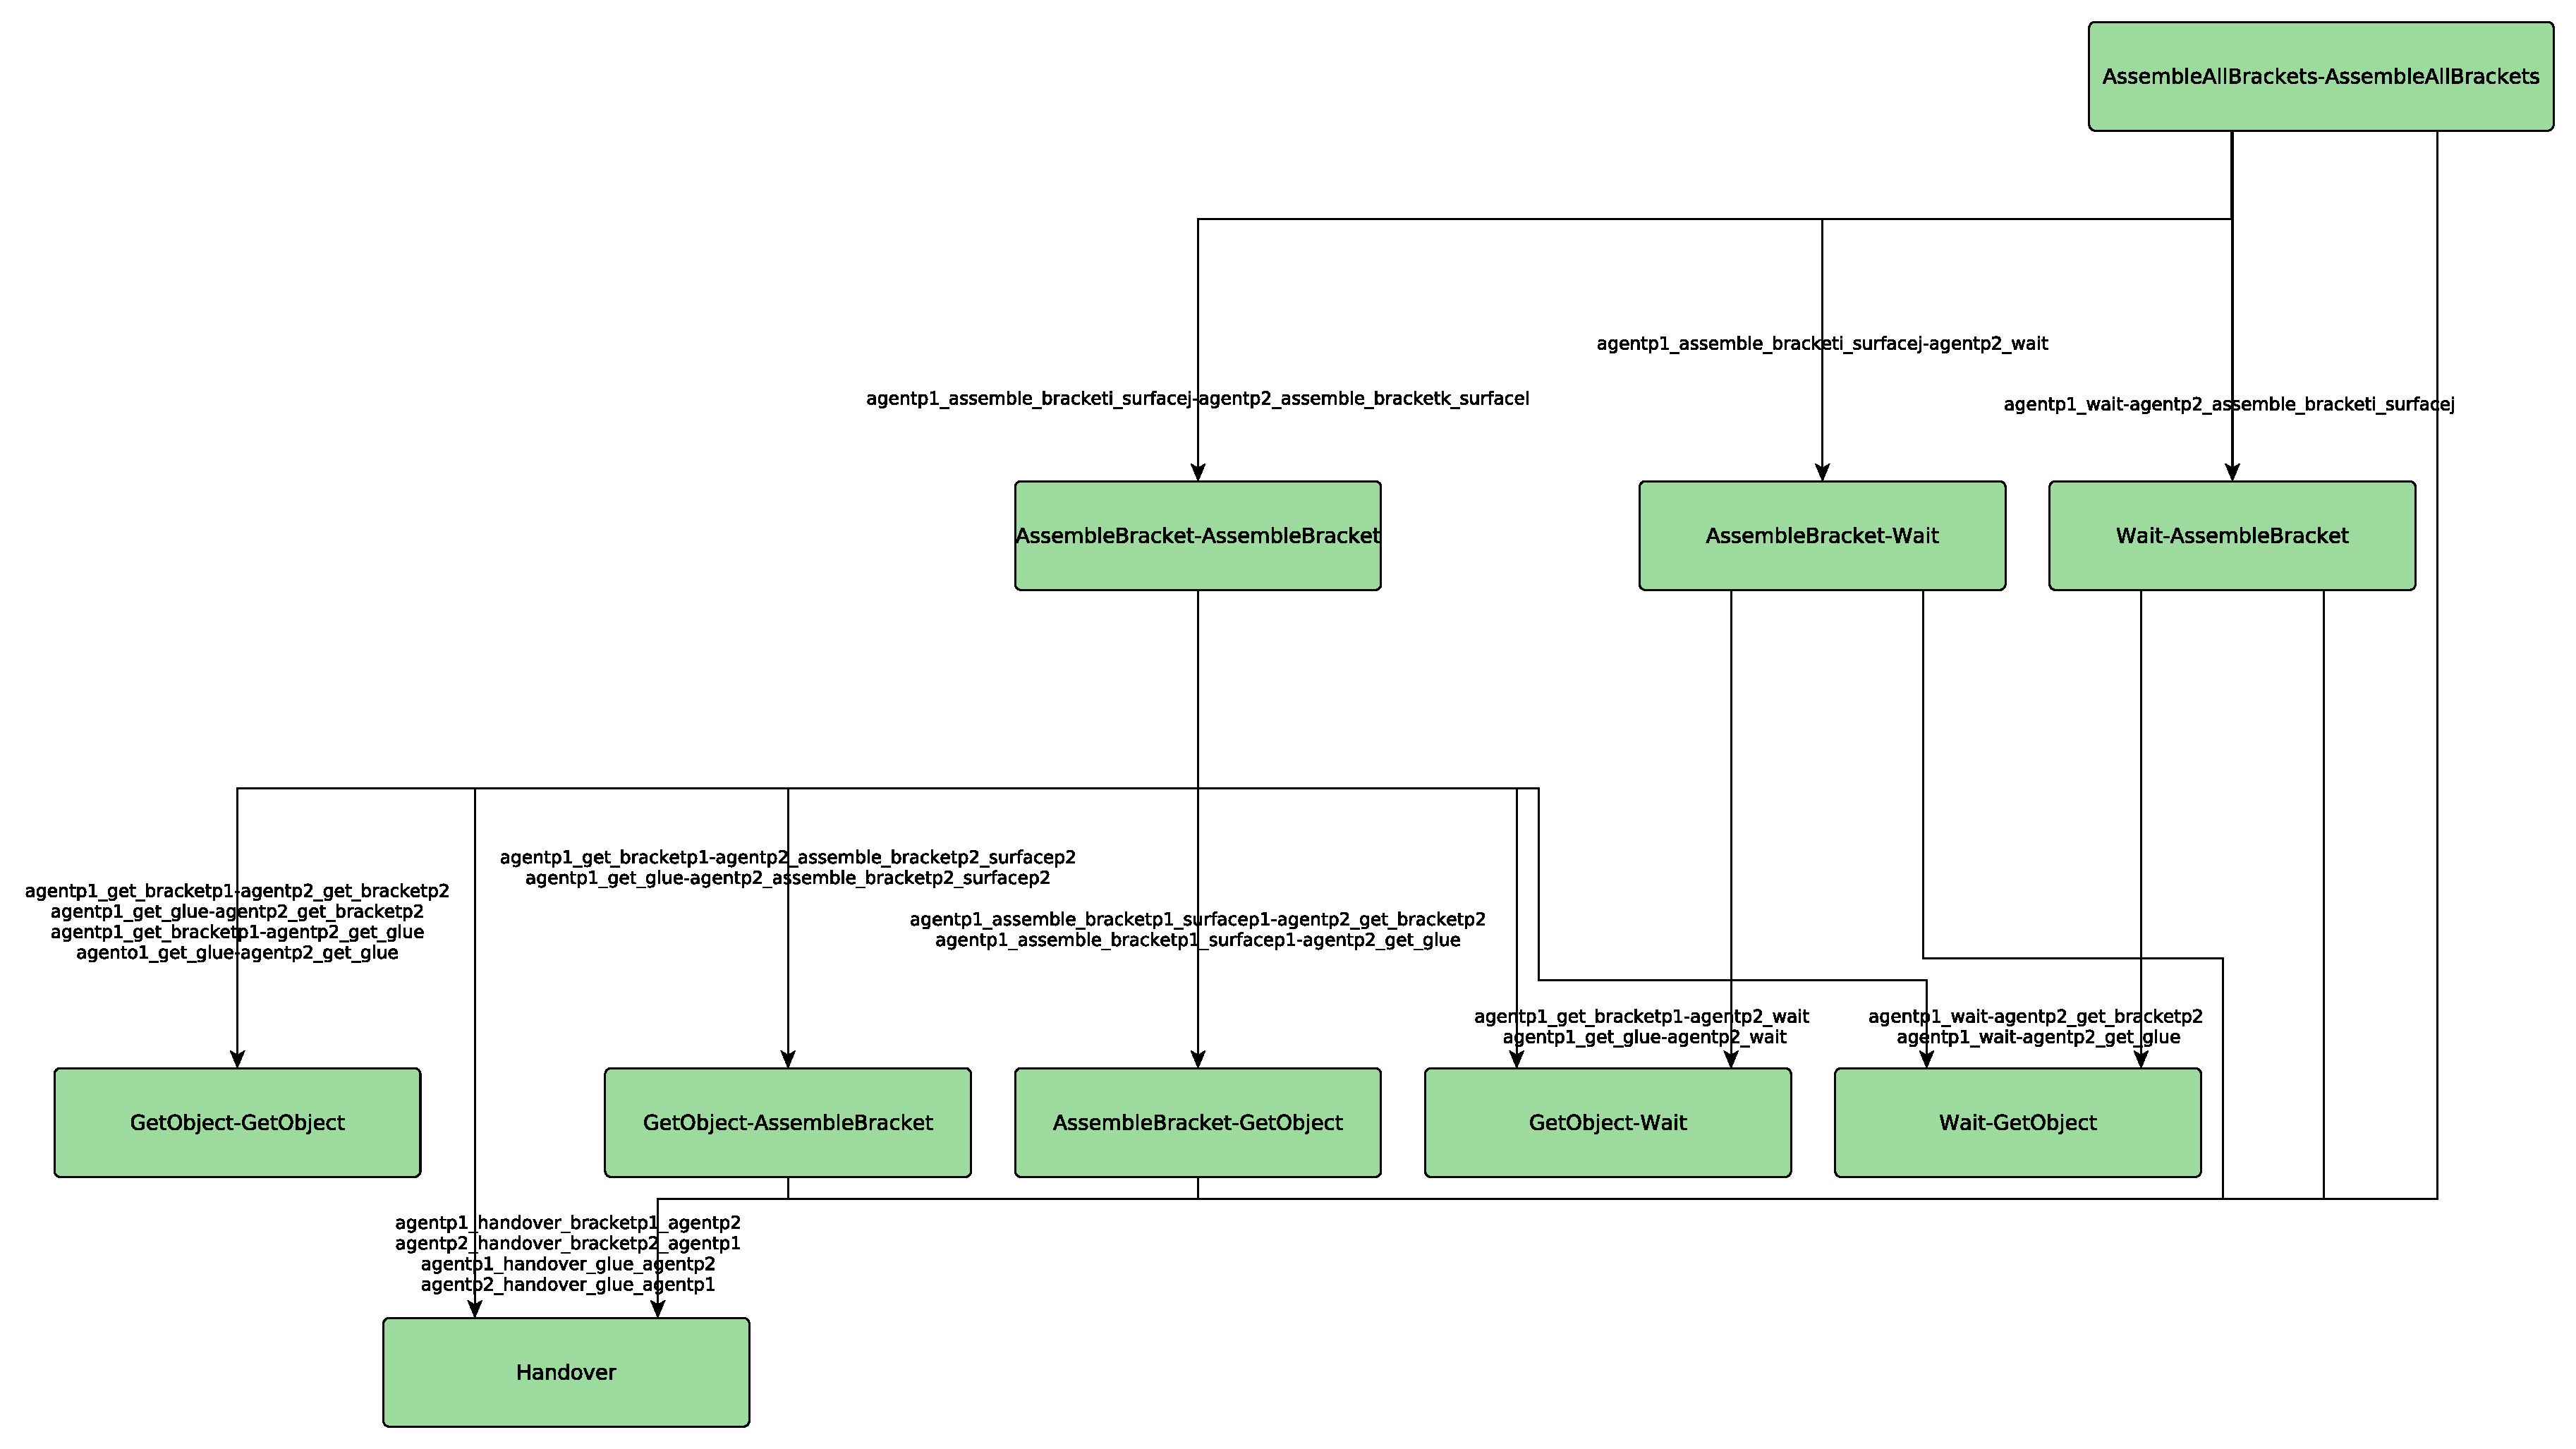
\includegraphics[scale=0.4]{img/coworker/mamdp/scenario_mamdp_architecture.pdf}
	\caption[MAMDP example: MAMDP model]{The image shows the architecture for the MAMDP of the example scenario. The various MAMDPs are represented as rectangles. The arrows show the links between hierarchical modules in the architecture. The label of an arrow shows the macro actions corresponding to the link.}
	\label{fig:mamdp-scenario_mamdp_architecture}
\end{sidewaysfigure}


\subsubsection{AssembleAllBrackets-AssembleAllBrackets}
\begin{itemize}
	\item $name: agent\_assembleallbrackets-agent\_assembleallbrackets$.
	\item		$par: \{agentp1,agentp2\}$.
		\begin{itemize}
			\item $par\_var(agentp1)=agentp1\_isAt$.
			\item $par\_var(agentp2)=agentp2\_isAt$.
		\end{itemize}

		The name of the parameters are changed, adding \textit{pi} at the end, where \textit{i} is the index of the agent. This allows to assign them in an unique way.
	\item $S:\;\{agentp1\_isAt,agentp2\_isAt, bracket1\_isAt,bracket2\_isAt,bracket3\_isAt,\\
	surface1\_status,surface2\_status,surface3\_status\}$. 
		\begin{itemize}
			\item $values(agentp1\_isAt):\{table,surface1,surface2,surface3\}$.
			\item $values(agentp2\_isAt):\{table,surface1,surface2,surface3\}$.
			\item $values(bracketi\_isAt):\{table,surface1,surface2,surface3,agentp1,agentp2\}\; \forall_{i=1}^3$. 
			\item $values(surfacei\_status):\{completed,other\_status\}\;\forall_{i=1}^3$.
		\end{itemize}
		\begin{itemize}
			\item $abstract\_values\_surfacei\_status:$ 
				\begin{itemize}
					\item $none: other\_status$.
					\item $cleaned: other\_status$.
					\item $glued: other\_status$.
				\end{itemize}
		\end{itemize}
		The state set is not very different, simply accounting for the presence of two agents.

	\item $A:\;\{agentp1\_assemble\_bracketi\_surfacej-agentp2\_assemble\_bracketk\_bracketl\}\;\forall_{i=1}^1 \forall_{j=1}^3
	\forall_{k=1}^3 \forall_{l=1}^3 \cup JointActions \cup WaitActions$.
	\item $JointActions=agentpi\_handover\_bracketj\_agentpl \; \forall_{i=1}^2 \; \forall_{j=1}^3 \; \forall_{l=1; l!=i}^3$.
	\item $WaitActions=(agentp1\_assemble\_bracketi\_surfacej-agentp2\_wait \; \cup \\
	 agentp1\_wait-agentp2\_assemble\_bracketi\_surfacej) \; \forall_{i=1}^3 \; \forall_{j=1}^3$.

	The action set is the cartesian product of the actions of the single models, plus actions to exchange brackets, plus actions where only one agent is acting.
	\item $M: A$.
	\item $G:\; \cup_{s:S}\; |\; \forall_{i=1}^3\; surfacei\_status=completed\;\text{AND}\\
	\forall_{i=1}^3\; \exists_{j}\;|\;bracketi\_isAt=surfacej\; \text{AND}\\
	\forall_{i=1}^3\; bracketi\_isAt \neq bracketj\_isAt$.
	\item $S_0:\; \cup_{s:S} \; \exists{1\leq i \leq 3}\; |\; surfacei\_status \neq completed$.

	The starting and goal states are the same as the single-agent model. Since the two models used to create the MAMDP are the same, the intersection and union of the states will be the same.
\end{itemize}


If we would create and solve a new MAMDP for each of these macros, we would create a great quantity of models. Fortunately, as previously said, we can reduce the number of models by creating generic sub-models for a macro that can be used when there are not parameters in common. In this case, we actually need to create a specific sub-MAMDP for every action of the type \textit{agentp1\_assemble\_bracketi\_surfacej-agentp2\_assemble\_bracketk\_surfacel}, where $i=j$ or $j=l$ (since they would have variables in common), plus a generic sub-MAMDP for all the other cases.

Also, in this example, all the MAMDPs for actions where the same bracket is assembled by two agents on different surfaces would not be created, as their goal states contain incongruent states (since a bracket can not be on two surfaces at the same time and a surface can not contain more than one bracket).

\subsubsection{AssembleBracket-GetObject}
Let us consider the AssembleBracket-GetObject MDP, deeper in the hierarchy. In this case, we will need to create a generic sub-MAMDP, plus specific MDPs for the macros \textit{agentp1\_assemble\_bracketi\_surfacej-agentp2\_get\_bracketi} and \textit{agentp1\_assemble\_bracketi\_surfacej-agentp2\_get\_glue}, since they share resources. We will show parts of this sub-MAMDP.  


\begin{itemize}
	\item $name: agent\_assemblebracket-agent\_getobject$.
	\item		$par: \{agentp1,bracketp1,surfacep1,agentp2,objectp2\}$.
		\begin{itemize}
			\item $par\_var(agentp1)=agentp1\_isAt$.
			\item $par\_var(bracket1)=bracketp1\_isAt$.
			\item $par\_var(surfacep1)=surfacep1\_status$.
			\item $par\_var(agentp2)=agentp2\_isAt$.
			\item $par\_var(object2)=objectp2\_isAt$.
		\end{itemize}

	\item $S:\;\{agentp1\_isAt, bracketp1\_isAt,surfacep1\_status, glue\_isAt, agentp2\_isAt, objectp2\_isAt\}$. 
		\begin{itemize}
			\item $values(agentp1\_isAt):\{surfacep1,other\_location\}$.
			\item $values(bracketp1\_isAt):\{agentp1,surface, other\_location,other\_agent\}$. 
			\item $values(glue\_isAt):\{agentp1,other\_location,other\_agent\}$. 
			\item $values(surfacep1\_status):\{none,cleaned,glued,completed\}$.
			\item $values(agentp2\_isAt):\{table,surface1,surface2,surface3\}$.
			\item $values(objectp2\_isAt):\{table,surface1,surface2,surface3,agentp2,other\_agent\}$. 
		\end{itemize}
		\begin{itemize}
			\item $abstract\_values\_objectp2\_isAt:$ 
				\begin{itemize}
					\item $greg=other\_agent$.
					\item $robot=other\_agent$.
				\end{itemize}	
			\item $abstract\_values\_bracketp1\_isAt:$ 
				\begin{itemize}
					\item $surfacei=other\_location \forall_{i=1}^n$ .
					\item $table=other\_location$.
					\item $greg=other\_agent$.
					\item $robot=other\_agent$.
				\end{itemize}	
			\item $abstract\_values\_glue\_isAt=abstract\_value\_bracketp1\_isAt$ 
			\item $abstract\_values\_agentp1\_isAt:$
				\begin{itemize}
					\item $surfacei=other\_location \forall_{i=1}^n$ .
					\item $table=other\_location$.
				\end{itemize}
		\end{itemize}

	\item $G:\; \cup_{s:S}\; |\; surfacep1\_status=completed\; \text{OR} \; objectp2\_isAt=agentp2$
	\item $S_0:\; \cup_{s:S} \; | \; surfacep1\_status \neq completed \; \text{AND} \; objectp2\_isAt \neq agentp2$

	The goal and starting states of the model are, respectively, the union and intersection of the single models.
\end{itemize}


\subsubsection{Handover}
Finally, to conclude, we show the special handover MAMDP, used for cooperative actions. Since this is a special model, not created by joining two single-agent MDPs, it will not follow the same rules, and instead it will be treated in a similar way as a single agent MDP.

\begin{itemize}
	\item $name: agent1\_handover\_object\_agent2$.
	\item		$par: \{agent1,object,agent2\}$.
		\begin{itemize}
			\item $par\_var(agent1)=agent1\_isAt$.
			\item $par\_var(agent2)=agent2\_isAt$.
			\item $par\_var(object)=object\_isAt$.
		\end{itemize}

	\item $S:\;\{agent1\_isAt, agent2\_isAt, object\_isAt\}$. 
		\begin{itemize}
			\item $values(agent1\_isAt):\{surface1,surface2,surface3,table\}$.
			\item $values(object\_isAt):\{agent1,agent2,other\_location\}$. 
			\item $values(agent2\_isAt):\{surface1,surface2,surface3,table\}$. 
		\end{itemize}
		\begin{itemize}
			\item $abstract\_values\_object2\_isAt:$ 
				\begin{itemize}
					\item $table=other\_location$.
					\item $surface1=other\_location$.
					\item $surface2=other\_location$.
					\item $surface3=other\_location$.
				\end{itemize}	
		\end{itemize}

	\item $A:\;\{agent1\_move\_location-agent2\_move\_location, agent1\_move\_location-agent2\_wait,\\agent1\_wait-agent2\_move\_location, \\ 
	agent1\_give\_object\_agent2-agent2\_receive\_object\_agent1\} \\ \text{where}\; location \in \{table,surface1,surface2,surface3\}$
	\item $G:\; \cup_{s:S} \; | \; object\_isAt=agent2$
	\item $S_0:\; \cup_{s:S} \; | \; object\_isAt=agent1$
\end{itemize}



\section{Enhancing Task Monitoring}
\label{sec:mamdp-plan_monitoring}

In section~\ref{sec:plan_management-plan_monitoring} we introduced the problem of task monitoring. We presented three different problematics: monitoring actions, monitoring tasks, and evaluating human engagement.

We presented a solution only for the problem of monitoring actions. In this section, we propose a strategy to monitor tasks and evaluate the human's engagement, based on the MAMDP model developed in this chapter. We are just starting to investigate this idea, and have not yet completed an implementation.

In general, a MAMDP proposes only the next action in the plan, which is not sufficient to manage plans and ensure synchronism. To deal with this problem, we can compute an horizon of $h$ actions from the MAMDP, building causal links between the nodes to create the stream structure introduced in chapter~\ref{chapter:plan_management}.

\subsection{Evaluating Human Engagement and Monitoring Tasks}
Understanding if a human is engaged in a task is equivalent to infer if its current intention is to achieve the task. As previously said, in section~\ref{subsec:intention-unknown_intentions}, normally, our Intention and Action Recognition module is not able to monitor joint goals. To solve this issue, while performing a shared plan, we create, in the Situation Assessment layer, a new intention for each MAMDP model in the domain. We associate to these intentions the linked MAMDP and the context node \textit{have a shared plan}, which is treated as evidence with a true value. We call these intentions \textit{plan intentions}.

We associate to each known intention a precomputed \textit{expected length}, which is the expected time to accomplish the linked goal.

Using the Intention and Action Recognition module, the robot can infer which is currently the most likely human intention. If the current intention equals the task to monitor, the robot infers that the human is actively working to complete its task.

 We consider the task, and the monitor procedure, as \textit{completed} when the linked MAMDP reaches a \textit{goal state}.

If the human is currently not involved in the monitored task there are three possibilities:
\begin{itemize}
	\item The human has momentarily interrupted the task. This can be inferred if the human is currently involved in another intention, which does not belong to the \textit{plan intentions}, and whose expected length is \textit{short}. In this case, the monitor procedure will not return an error until a predefined \textit{allowed time}.
	\item The human has abandoned the task.  This can be inferred if the human is currently involved in another intention, which does not belong to the \textit{plan intentions}, and whose expected length is \textit{long}. The monitor will return an error. 
	\item The human is performing another task in the shared goal. This can be inferred if the human is currently involved in another intention, which belongs to the \textit{plan intentions}. In this case the monitor will return an error. 
\end{itemize}




 

\part{The Robot Teacher} % Main chapter title

\label{part:robot_teacher} % Change X to a consecutive number; for referencing this chapter elsewhere, use \ref{ChapterX}

\lhead{Part IV. \emph{The Robot Teacher}} % Change X to a consecutive number; this is for the header on each page - perhaps a

We can imagine robots in several ways. The more realistic persons will imagine the robot as a tool, able to execute repetitive, high-precision tasks, reducing humans' effort. The more imaginative persons will instead think of the kind of robots that we can see in science fiction literature or movies: autonomous agents, able to reason and to act almost as humans. In general, we would think of the robot as some sort of `programmable' entity. We teach the robot, through our code and algorithms, to execute its task.

In the last years, actually, there is an increasing interest in `inverting this role' by having robots act as teachers, particularly with children. Some studies, like \cite{movellan2009sociable}, have shown that a robot teacher can actually positively impact on the learning process of children.

In this part, we introduce the problem of the \textit{robot teacher}, where the robot needs to explain a user how to execute a task and then guide him in its achievement. We are particularly interested in adapting this process to the \textit{knowledge} of users in the tasks to perform, by explaining more in-depth processes where the user has less \textit{expertise}, and quickly tasks that user has already accomplished several times. While we are calling this problem \textit{robot teacher}, these mechanisms can benefit any cooperative application where the robot is acting as leader, and needs to explain a cooperative plan to its partners.  

Chapter~\ref{chapter:knowledge} will explain how we model the knowledge of a user in a task to adapt the plan explanation and management processes. Chapter~\ref{chapter:teacher_results} shows a user study performed to validate our approach.

\chapter{Adapting Plan Management to Human Knowledge} % Main chapter title

\label{chapter:knowledge} % Change X to a consecutive number; for referencing this chapter elsewhere, use \ref{ChapterX}



\lhead{Chapter 8. \emph{Human Knowledge}} % Change X to a consecutive number; this is for the header on each page - perhaps a shortened title
  
In this chapter we show how we use human knowledge to adapt the plan explanation and managent capacities of our system. Section~\ref{sec:knowledge-intro} introduces the subject, while section~\ref{sec:knowledge-overview} explains the basics of our approach to model knowledge. Section~\ref{sec:knowledge-adapting_knowledge} shows how human knowledge can be used to adapt the planning capacities of HATP. Finally, sections~\ref{sec:knowledge-plan_presentation} and \ref{sec:knowledge-plan_management} respectively describe how the robot can explain plans in a human-aware way, by taking into account the knowledge of the human, and how it can guide the human in the execution of the task, by modifying our plan management algorithm.


\section{Introduction}
\label{sec:knowledge-intro}

In section~\ref{subsec:plan_management-robot_leader} we introduced a simple algorithm to explain a plan to a user. The problem of explaining a plan in a `naive way', by simply verbalizing all of its actions, is that the explanation can be long and not interesting. 

Let us imagine a robot explaining a human how to change the tires of a car. The robot could start by telling the human how to loosen the nuts of a wheel. It could tell the human to take a wrench, to apply it to a nut, and to turn it counter-clockwise. The human will need to loosen several nuts. If for each nut the robot will explain the user again to apply the wrench and turn it counter-clockwise, the explanation will be much longer than what is needed. Imagine the robot explaining every single small operation of a large plan. The result could be a nightmare for the human! A more natural way to teach this task would be explain how to loosen the first nut, and then just ask the human to loosen the others, without going in-depth in each operation.

This idea is validated by research on Intelligent Tutoring Systems \citep{brusilovskiy1994construction}  and on e-learning \citep{brusilovskiy2005}, which has proven  the necessity of keeping and updating a model of the learner's knowledge to efficiently teach a task.

This idea has still not been widely investigated in robotics. \cite{Sorce2015} show a system where the robot can learn shared plans from a human, and then transfer this knowledge to non-expert humans. The explanations of the robot are joined by a video, representing what the robot perceived when it learnt the task, to give more information to the human.

Even when the robot is a coworker, and not a teacher, research \citep{Lallee2013} suggests that collaborative plans should be fully communicated in order to sustain effective cooperation. The preferred method of communication in complex tasks is usually language \citep{Warneken2006,Warneken2007}.

In the following sections, we will present our approach, where we adapt plan explanation and management to the knowledge of users.

% \section{Plan Negotiation}
% \label{sec:plan_management-negotiation}
% Once the robot has presented the plan to his collaborators, it can start a negotiation phase. 

% We introduce a simple negotiation algorithm, that starts with the robot asking humans for approval of the plan, inquiring what is wrong in case of disagreement. We handle two different human requests. First, the user can express his preferences, either to perform a task previously assigned to the robot or to not perform a task assigned to him. The other possibility is to inform the robot that the user cannot perform an action. The system will store these information and try to find a new plan, taking them into account, before starting a new explanation and negotiation phase.


% In a collaborative scenario, all the agents must agree on the shared plan. If there is a disagreement the agents might negotiate to find a nother solution.  This problem has been studied, for example, in \cite{fabregues2014hana}, where the authors present the \HANA system, an architecture that allows agents (robots and humans) to negotiate in competitive and cooperative settings. In HANA agents interact during the whole planning process, proposing solutions while they keep searching for better plans. During this process agents agree on performing specific tasks, which prunes the search space of feasible plan.


\section{Overview}
\label{sec:knowledge-overview}
\subsection{Modeling Knowledge}
Before explaining our algorithms, we introduce a new attribute (as explained in ~\ref{sec:belief_management-overview}) among our symbolic facts: the knowledge of a human in a task.

This attribute is represented as a tuple $(human, task, parameters, value)$, where $human$ is a string identifying the subject of this attribute, $task$ is the name of the related task, $parameters$ is a list of relevant parameters used to describe the knowledge in the task, and $value$ is the level of knowledge in the task. Knowledge values can be assigned from the set $[new, beginner, intermediate, expert]$.  For example, we can represent the fact that Bob knows very well how to fix a wheel to a car with the tuple $(Bob, fix\_wheel, car, expert)$. 

Parameters can be deeply linked to the knowledge of a task. In general, we can divide task parameters in two categories:
\begin{itemize}
\item Class-Link. In some situation, knowledge of a task is not linked to the specific instance of a parameter, but to a whole class. For example, we can imagine that if Bob knows how to paint the living room, he will know how to paint every room in a house. We could represent this attribute as $(Bob, paint, house\_room, expert)$. We can notice that the parameter, in this case, is $house\_room$, representing the class of rooms belonging to a house, and not $living\_room$.
\item Instance-Link. In other cases, instead, knowledge of a task is deeply linked to specific instances of parameters. For example, knowing how to fix the motor of a specific car, would not necessary translate in knowing how to fix the motor of every car.
\end{itemize}

We can also consider some tasks as \textit{common knowledge}, expecting every human to be able to perform them, like, for example, putting ingredients in a bowl. These tasks will be tagged as \textit{common knowledge} and considered as known by any user, no matter the parameters. 

\subsection{Maintaining Human Knowledge in a Task}
%How human update their knowledge
We define four task-knowledge levels for humans, that will lead to different behaviors from the robot.

\begin{itemize}
\item \textit{New}. This value will be used for tasks which have never been performed by the user. If the user observes the task being executed, with an explanation of it, or if he performs it himself, the value will be changed to \textit{beginner}. However if the user observes the task being executed without any explanation, we keep the level as \textit{new} since we consider that he might not have received enough information to link the observed movements to the task.
\item \textit{Beginner}. This value will be used for users who have already achieved the task but may still need explanations to perform it again. If the user successfully performs the task a second time, without asking for explanations, the value is changed to \textit{intermediate}, otherwise it is changed to \textit{new}.
\item \textit{Intermediate}. This value will be used for users who are able to perform the task without guidance. If a \textit{beginner} user successfully performs the task without guidance again, the value is changed to \textit{expert}. In case of failure, it is downgraded to \textit{beginner}.
\item \textit{Expert}. This knowledge level will be used for users who are able to perform the task without guidance and are experienced enough to explain it to a third party. If the user fails in performing the task, he will be downgraded to \textit{intermediate}.
\end{itemize}

Using the knowledge of a task of a human, the system is able to adapt plan generation, explanation, and monitoring to that user.


\subsection{Architecture}
This process was implemented by integrating a new module in the Plan Management layer's architecture, presented in chapter~\ref{chapter:plan_management}, which we called `Plan Explanation'. This module receives as input a shared plan, from the Plan Manager, and the current knowledge of the humans involved in the plan, from the Situation Assessmen layer. With these information, it will adapt the knowledge of users to explain the shared plan. Information about human's knowledge will be used also by the Plan Manager module to adapt the plan management algorithm, as we will explain in the following sections.

The modified architecture of the Plan Management layer is shown in figure~\ref{fig:knowledge-knowledge_architecture}. This work was presented in~\cite{milliez2016using}.

\afterpage{\clearpage}
\begin{sidewaysfigure}[ht!]
  \centering
  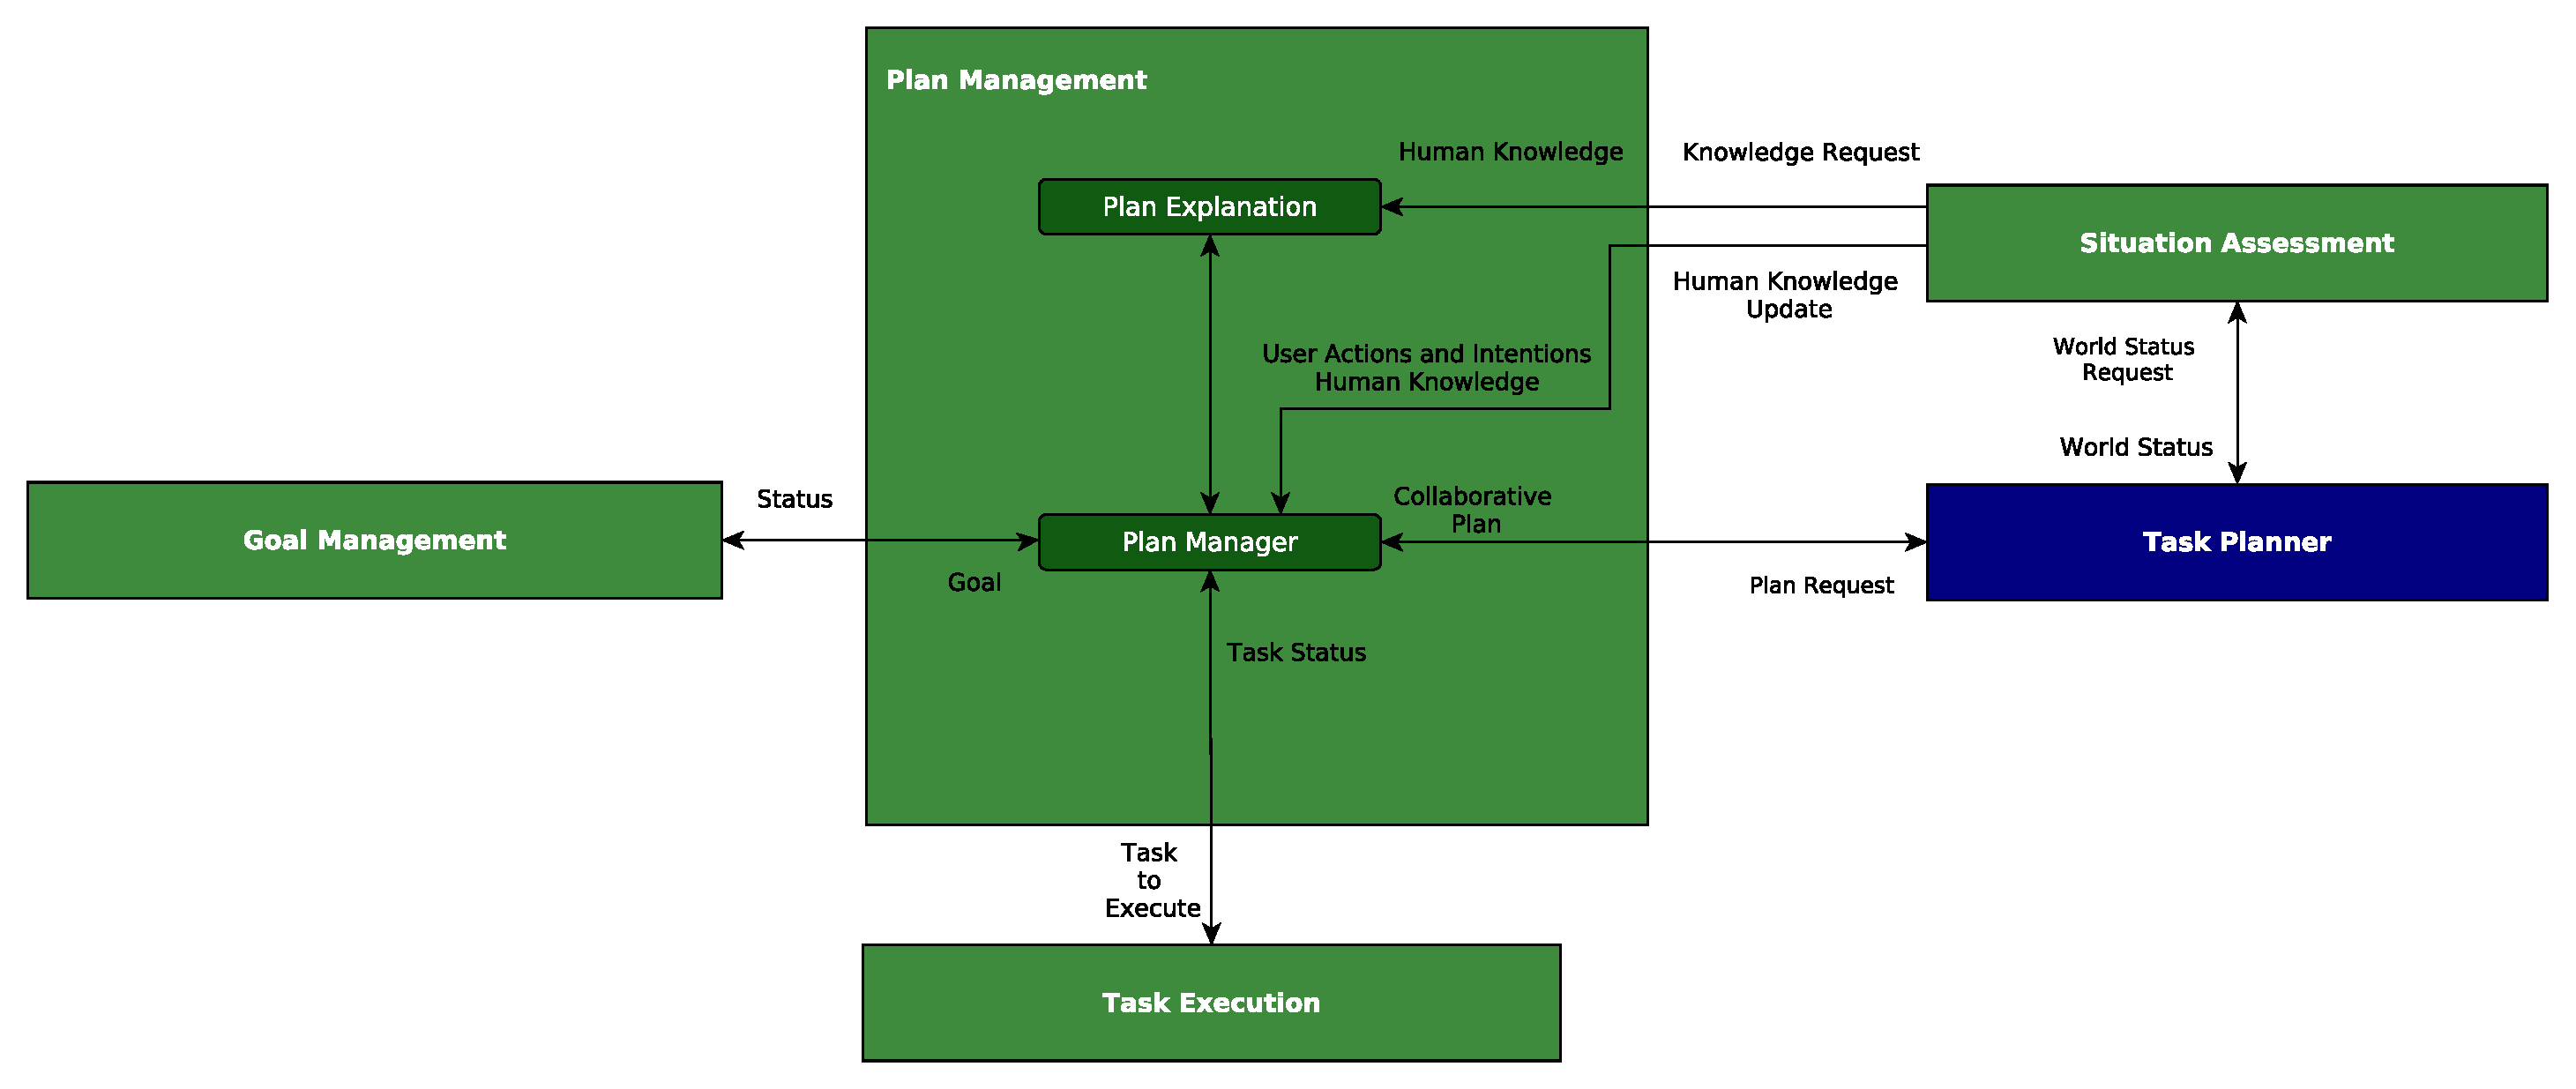
\includegraphics[scale=0.5]{img/teacher/knowledge_architecture.pdf}
  \caption[Integration of the human knowledge in the Plan Management layer]{The architecture of the Plan Management layer integrated with the Plan Explanation module, and with human's knowledge information. Light green rounded rectangles represent modules, while dark green rectangles layers. The Task Planner is shown as a blue rectangle to indicate that it is a module external to the system. Arrows represent message exchanged between components, with the label detailing the message.}
  \label{fig:knowledge-knowledge_architecture}
\end{sidewaysfigure}


\section{Adapting Plan Generation to Human Knowledge}
\label{sec:knowledge-adapting_knowledge}
When interacting with humans, it is important to take into account others' knowledge and capacities when planning. We consider two different policies for our planner: $teaching$, where the planner will look for plans not known to the human, in order to teach him different ways to achieve a task; and \textit{efficiency}, where the robot will try to maximize the number of human tasks known when creating a plan. These ideas were represented as social rules.

To illustrate these new social rules let us consider an example where a human and a robot have to cook an apple pie. We can consider all the basic actions of this domain (pick, place, cut, etc.) as \textit{common knowledge}, but the human might not know how to perform all the higher level tasks involved. If our policy favors \textit{teaching}, 
the plan should should choose a decomposition with tasks where the human has a low knowledge level. On the other hand, if our policy is \textit{efficiency} the planner should allocate to the human tasks where he is more competent, so that explanations and mistakes are reduced. Using this rule, the robot is able to adapt its plan generation to the knowledge of the user concerning tasks contained in the shared plan. In figure \ref{fig:knowledge-adapting_plan_knowledge} we show an example of plan adaptation for this task with the two policies, using the mental model in table \ref{table:knowledge-apple_pie_human_knowledge}

 
 \begin{table}
\centering
\scriptsize
\renewcommand{\arraystretch}{1.3}
\begin{tabular}{|c|c|}
\hline
Task & Knowledge Level \\ \hline \hline
Cook(ApplePie) & New \\ \hline
PrepareDough(Bowl Mould) & New \\ \hline
PrepareMixture(Bowl Mould) & Intermediate \\ \hline
PrepareFruits(Apple Bowl Mould) & Intermediate \\ \hline
Bake(Mould) & Intermediate \\ 
\hline
\end{tabular}
\caption[Mental model for a human in the Cook Apple
 scenario.]{Mental model for a human in the Cook Apple
 scenario in figure \ref{fig:knowledge-adapting_plan_knowledge} }
 \label{table:knowledge-apple_pie_human_knowledge}    
\end{table}



\begin{figure}[ht!]
 \centering
  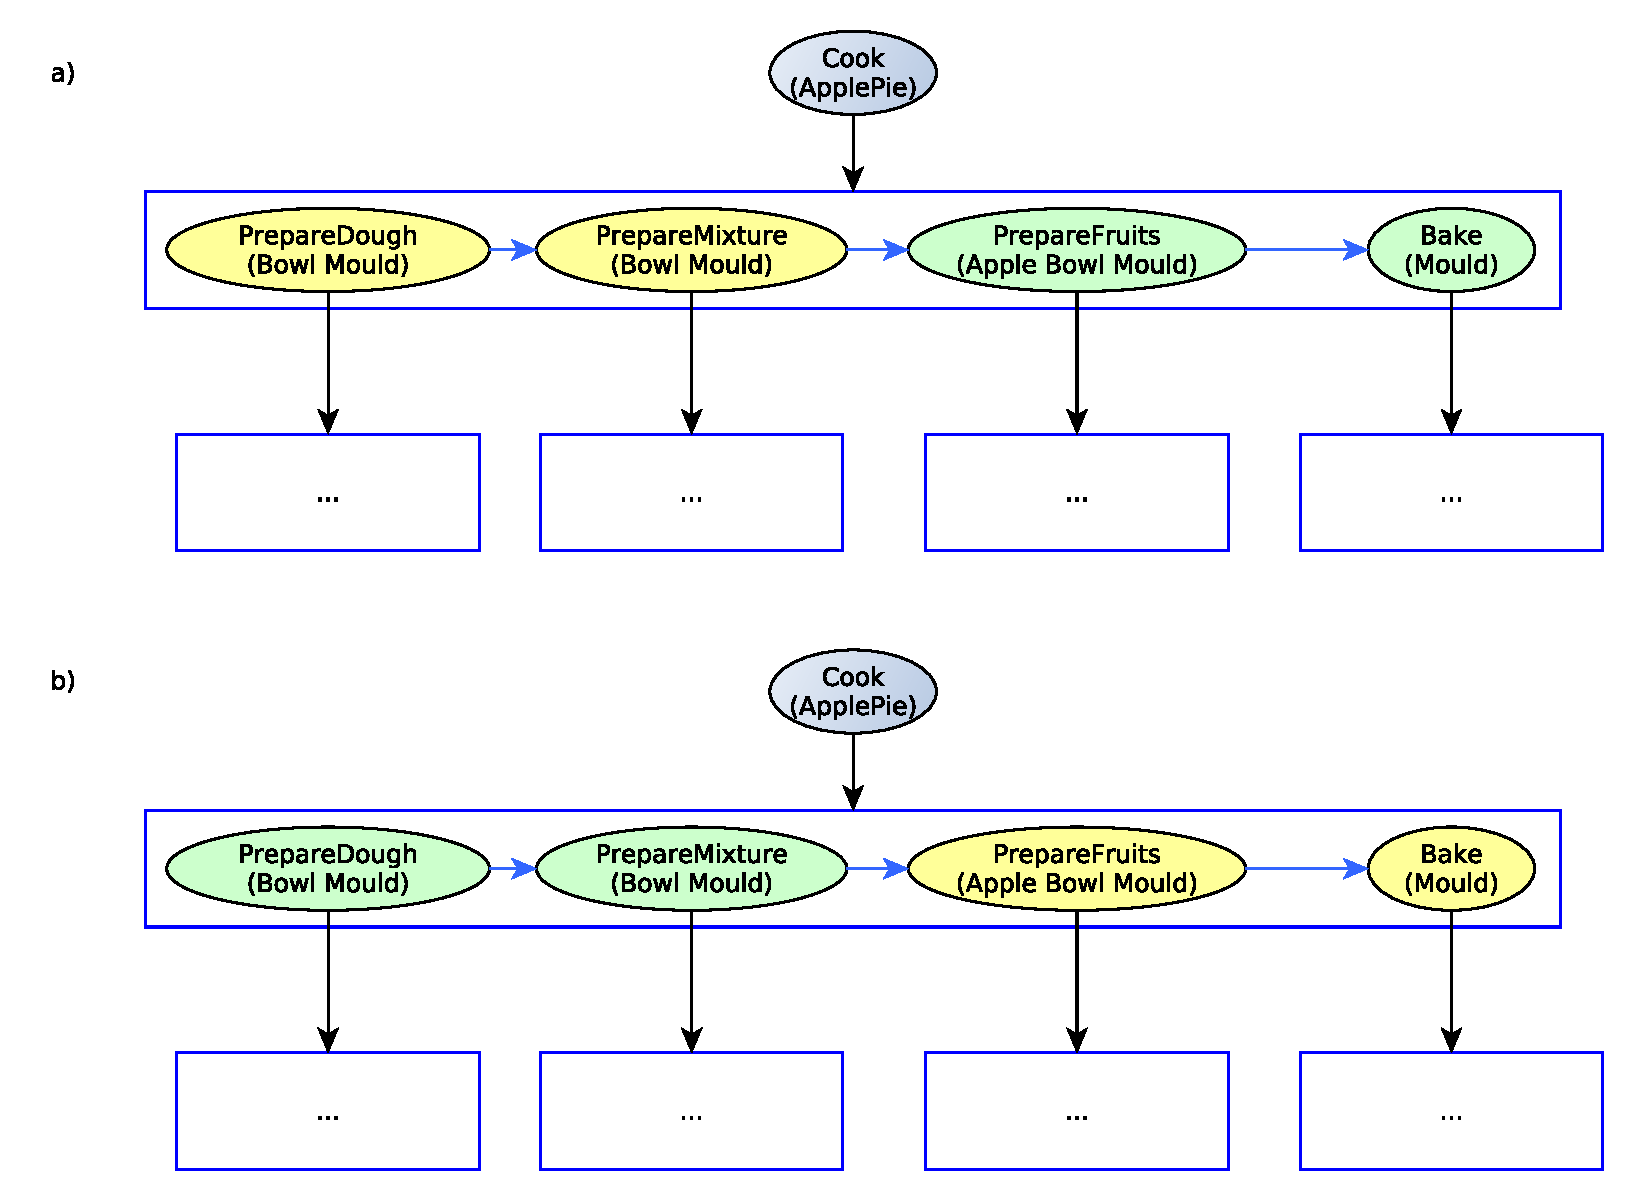
\includegraphics[scale=0.5]{img/teacher/adapting_plan_knowledge.pdf}
 \caption[Allocation of tasks of a plan to cook an Apple Pie for two agents]{Allocation of tasks of a plan to cook an Apple Pie for two agents, a robot and a human, using the knowledge values in table \ref{table:knowledge-apple_pie_human_knowledge}. A) shows an \textit{efficiency} policy for this task, while b) shows a \textit{teaching} policy for the same task. Blue ellipses represent tasks involving both agents, green ellipses represent tasks assigned to the human, and yellow ellipses tasks assigned to the robot. Each decomposition is grouped in a blue rectangle. Black arrows link a method to its decomposition, while blue arrows represent casual links. Squares with a `...' label represent decompositions that are not shown in this picture.}
 \label{fig:knowledge-adapting_plan_knowledge}
 \end{figure}



To properly compute the cost of a plan, the planner will also upgrade accordingly the knowledge of a task once it is added to the plan. This allows the \textit{efficiency} policy to prefer plans with repetitive decompositions, that are assigned to the same user, over plans with more variable decompositions, where repetitive tasks are assigned to different agents.

% The planner can receive information produced from a dialog system that allows to negotiate plans, as explained in section \ref{sec:plan_management-negotiation}. Using this system, the preference and abilities of users are recorded in the Situation Assessment layer. 
% If a user is not able to perform a certain task, the planner will never chose this action for him. If he user prefers to perform, or not to perform, a specific task, the planner will update the cost functions accordingly with a reward or penality to assign that task to him.


\section{Plan Presentation}
\label{sec:knowledge-plan_presentation}
Before executing the plan, the robot will present the goal and the proposed allocation of high-level tasks to give a global view of the chosen strategy. Standard natural language generation is used, as shown in table \ref{table:knowledge-pie-present}. 
In some situations, the plan will be too long to explain it in one step to a user, who could then be confused or annoyed. For this reason, when presenting the plan, the robot will verbalize only the first $N$  highest level tasks. We have chosen $N$=$3$ based on our own experience during tests with the system, but we can imagine to adapt it to the complexity of the domain, or even to specific users. The robot will present the first steps of the plan, and then execute them. Once these tasks have been executed, the robot will repeat the present/execute process until the plan is completed or aborted.
 
 \begin{table}
 %\vspace{-10pt}
\centering
\scriptsize
\renewcommand{\arraystretch}{1.3}
\begin{tabular}{c|c}
   agents(root) $+$ have\_to $+$ root  & "We have to cook an apple pie." \\
   \hline
   introduce\_presentation & "I will tell you the steps." \\
   \hline
   agents(child[0]) $+$ first $+$ child[0] & "You will first fetch the ingredients," \\
   \hline
   then $+$ agents(child[1]) $+$  child[1] & "Then I will assemble the apple pie," \\
   \hline
   finally $+$ agents(child[2]) $+$  child[2] & "Finally, you will bake \\
   & the apple pie in the oven." \\
\end{tabular}
\caption[Presentation of a plan to cook an apple pie]{Presentation of a plan to cook an apple pie. Root is the root of the HTN tree and child is a list with its children.}
 \label{table:knowledge-pie-present}    
\end{table}


\section{Plan Management and User Knowledge}
\label{sec:knowledge-plan_management}
We start this section by showing how we adapted our plan management algorithm to take into account the human's knowledge in the task. After showing the algorithm, we will explain it. During this algorithm we will sometimes discuss about the consequence of a user \textit{failing} at executing a task. We deduce that a user fails if he executes a different action than the one the robot is expecting, or if he does not execute any action for a long period of time (determined by setting a threshold).

%\begin{algorithm}
\begin{algorithmic}[1]
\For{n$:=$nodes.start to n$:=$nodes.end}
  \If{$agents$(n) = \{robot\}}\label{alg:onlyRobotStart}
      \If{$children(n) \neq \emptyset$ $\wedge$ $user\_kn(n)$ = new\par
        \hskip\algorithmicindent $\wedge$ $teachPolicy$}
          \State $execute\_tree(children(n))$
            \State $user\_kn(n) :=$ beginner
        \Else
          \State $execute(n)$
        \EndIf\label{alg:onlyRobotEnd}
    \ElsIf{$user\_kn(n)$ = new}\label{alg:newStart}
      \State $explain(n)$
        \If{$children(n)$ $\neq \emptyset$}
            \State $execute\_tree(children(n))$
            \State $user\_kn(n)$ $:=$ beginner
        \Else
          \State $monitor(n)$
        \EndIf\label{alg:newEnd}
    \ElsIf{$user\_kn(n)$ = beginner}\label{alg:beginnerStart}
        \If{$propose\_explain(n)$}
            \State $user\_kn(n)$ $:=$ new
            \State $(\dots)$ \Comment{Same process as new}
        \Else
            \State $monitor(n)$
        \EndIf\label{alg:beginnerEnd}
    \ElsIf{$user\_kn(n)$ = intermediate\par
    \hskip\algorithmicindent $\vee$ $user\_kn(n)$ = expert}\label{alg:interStart}
        \State $monitor(n)$
    \EndIf\label{alg:interEnd}
\EndFor
\end{algorithmic}
%\caption{$execute\_tree(n)$}

%\end{algorithm}

\begin{itemize}
\item \textit{$execute\_tree(n)$} is the main plan management function. The function receives as argument \textit{$nodes$}, a list of nodes initially filled with the root's children.
\item \textit{$teachPolicy$} is a boolean that defines if we are in teaching or efficiency mode.
\item \textit{$agents(n)$} returns the agents involved in the node \textit{n}.
\item \textit{$verbalize(n)$} will verbalize the current task, using the node context to present it (e.g. using sequential relations such as first, then or finally according to the node position in the list).
\item \textit{$user\_kn(n)$} returns the knowledge level of the user concerning the task \textit{n}.
\item \textit{$propose\_explain(n)$} will lead the robot to propose an explanation for the current task. If the user accepts the explanation it will return true, and otherwise false.
\item \textit{$explain(n)$} launches a procedure to explain the current task to the user. This procedure could be implemented as a script to launch a video, an explanation speech or even to ask an expert to explain the task.
\item \textit{$monitor(n)$} starts monitoring the proper execution of the current node. If the request returns a success, the function will upgrade the user's knowledge and the \textit{$execute\_tree$} function will continue. In case of failure, the function will downgrade the user's knowledge, exit the \textit{$execute\_tree$} function, and return a failure that will result in a replan request and a new execution if a plan is found.
\item \textit{$execute(n)$} works in a similar way to the monitor but sends a request to execute the node by the robot.
\end{itemize}
 
\subsection{Explanation of the plan management algorithm}
This plan management algorithm is based on the structured plan tree computed by the task planner, and on the tasks' knowledge values in the user models. We explore this tree with a pre-order strategy. The algorithm will analyze each node, with several possible outcomes:

\subsubsection{Only the robot is involved (lines ~\ref{alg:onlyRobotStart}-~\ref{alg:onlyRobotEnd})}
If the robot is the only agent in charge of the current node, the collaborator has a knowledge level equal to \textit{new} for the current task,
and the chosen policy for the interaction is teaching, then the robot will execute the subtasks in `demonstration mode, meaning that it will verbalize each child task before performing it.

Once the task has been executed, the robot updates the human's knowledge on the current node to \textit{beginner}. The same process will be applied to the tasks' children.  Using this process, the robot will verbalize each (and only) task that needs to be learned by the collaborator.

If the robot is in charge, but the human collaborator's knowledge on the task is different from \textit{new}, or the current policy is efficiency, the robot will verbalize only the high-level task it performs.

If the human is involved in the current node, the robot's behavior will depend on the human's knowledge level for the task, since he might need explanations.  Explaining a task could be done in several ways: showing a video, asking an expert to explain the it or simply verbally guiding the user, step by step.
\subsubsection{The collaborator's knowledge level on the task is \textit{new} (lines~\ref{alg:newStart}-~\ref{alg:newEnd})}
If the human has the level $new$ for the current task, we explain it.
When verbally guiding the user, if the current node has only one child, we  go deeper in the tree and apply again the corresponding behavior according to the knowledge level. If the current node is actually an operator (a leaf), the system monitors the current action execution. In case of success, the knowledge level for the task is upgraded to \textit{beginner}.

% if beginner
\subsubsection{The collaborator's knowledge level on the task is \textit{beginner} (lines ~\ref{alg:beginnerStart}-~\ref{alg:beginnerEnd})}
 If the human has the level \textit{beginner} for the current task, we ask if he needs explanations. If so, we downgrade his knowledge level to $new$ on the current task and apply the same process as the previous paragraph. If the user refuses explanations, we simply monitor the execution of the current node. In case of success, the knowledge level for the current task is upgraded to \textit{intermediate}. This knowledge level will also be used as default. This way, when the robot does not know the knowledge level of an agent concerning a task, it will just ask him if he needs an explanation and adapt its behavior accordingly.

% if intermediate
\subsubsection{The collaborator's knowledge level on the task is \textit{intermediate} (lines~\ref{alg:interStart}-~\ref{alg:interEnd})}
 If the human has the level \textit{intermediate} for the current task, we verbalize it without proposing explanations, since he has already  succeeded with the plan at least once without help. Also, we do not go deeper in the tree and directly monitor the current task. If the user  fails, we downgrade his knowledge to \textit{beginner}, otherwise we upgrade it to \textit{expert}.

% if expert
\subsubsection{The collaborator's knowledge level on the task is \textit{expert} (lines~\ref{alg:interStart}-~\ref{alg:interEnd})}
 In case of an \textit{expert} knowledge level on the current task, we  proceed as for the previous knowledge level, downgrading the level to \textit{intermediate} if the user makes a mistake and keeping the \textit{expert} level if he performs the task as expected.



\subsection{Replanning}
When the plan manager reports a failure, the system needs to look for a new plan. If possible, we would like to create a plan which contains the same high-level task allocation. Sometimes, when the Plan Manager fails, there is no need to completely change the plan. Instead, it might be sufficient to repair only a part of it. For example, we can imagine a scenario where a human might execute task $t_1$ using resource $r_1$ or $r_2$. Perhaps the robot computed a plan where the human will use resource $r_1$, while itself will use $r_2$ to achieve another task.

If the human does not follow this plan, and uses $r_2$ to compute its task,  it might be faster to just repair the plan, looking for a solution where the task allocation is the same, but the robot uses $r_1$ instead to achieve its task. This way, we avoid starting a new explanation phase, which could look useless and not natural to the human collaborator.

%  We deal with this issue in different ways in HATP and HAPP.

In HATP, we introduce a new social rule. When presenting a plan, we record which nodes have been presented and assigned to each agent. While planning, we penalize plans with a different task allocation. This way, the planner will prefer to use the same task allocation, but will change it if needed, for example because, using the previous task allocation, the goal is no longer achievable.

%In HAPP, we can just perform a partial replan, by interrogating the currently active MMODP.  


 
\chapter{Experiments and Results} % Main chapter title


\lhead{Chapter 9. \emph{Robot Teacher Results}} % Change X to a consecutive number; this is for the header on each page - perhaps a

\label{chapter:teacher_results} % Change X to a consecutive number; for referencing this chapter elsewhere, use \ref{ChapterX}


 \section{Scenario}
\label{sec:teacher_results-scenario}
To test our system, we have chosen a scenario where a human is trying to prepare two desserts, an apple pie and a banana pie, without knowing their recipes. The robot's goal is to teach the human how to prepare the two dishes, by explaining him the task that he has to execute, and by guiding him during this process, as shown in figure \ref{fig:teacher_results-scenario}. 

\begin{figure}[ht!]

 \centering
 \begin{tabular}{cc}
  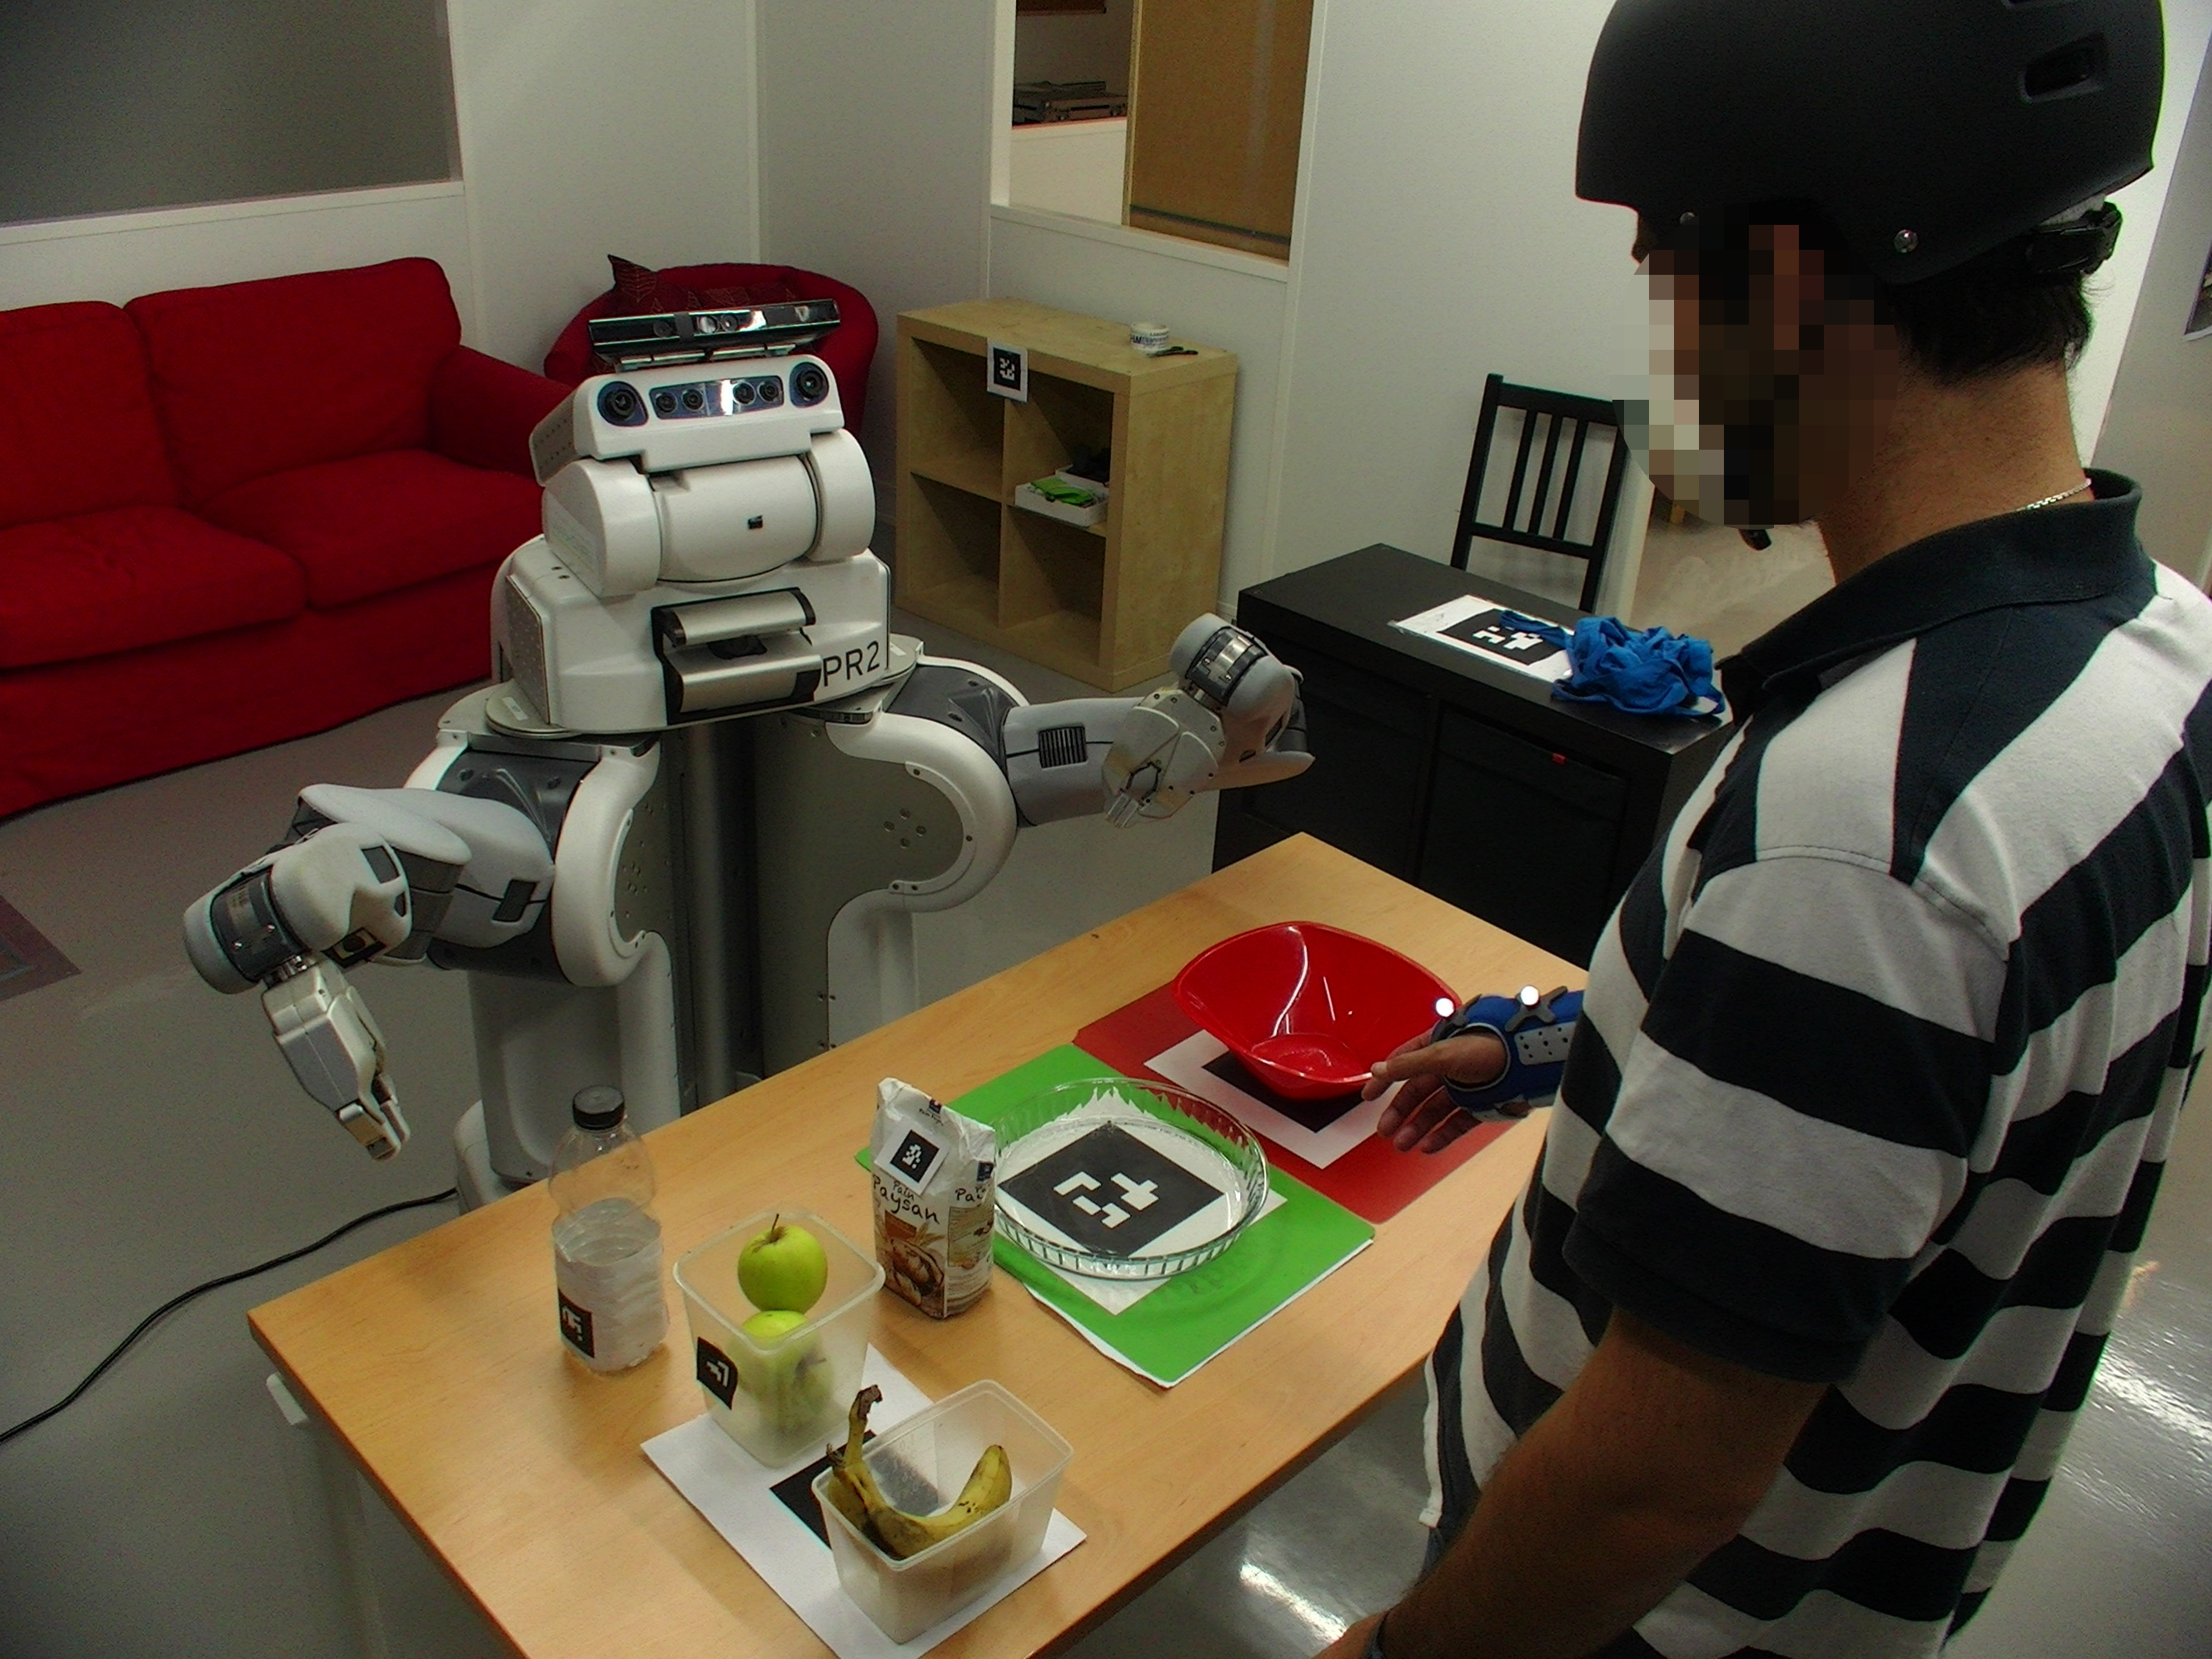
\includegraphics[width=0.29\textwidth]{img/teacher/scenario.JPG}
 \end{tabular}
 \caption{Illustration of the cooking pies scenario}
 \label{fig:teacher_results-scenario}
 \end{figure}

We created a domain to represent this scenario, and tested it using the previously explained \textit{efficiency policy} and HATP as task planner. The process of cooking an apple pie involves five main tasks. We imagine that, in our set-up, the robot is not able to execute the \textit{PrepareDough} and \textit{PrepareFruits} tasks, since it can not reach the needed ingredients. HATP produces a plan, allocating the tasks as follows:

\begin{figure*}[ht!]
 \centering
 \begin{tabular}{cc}
  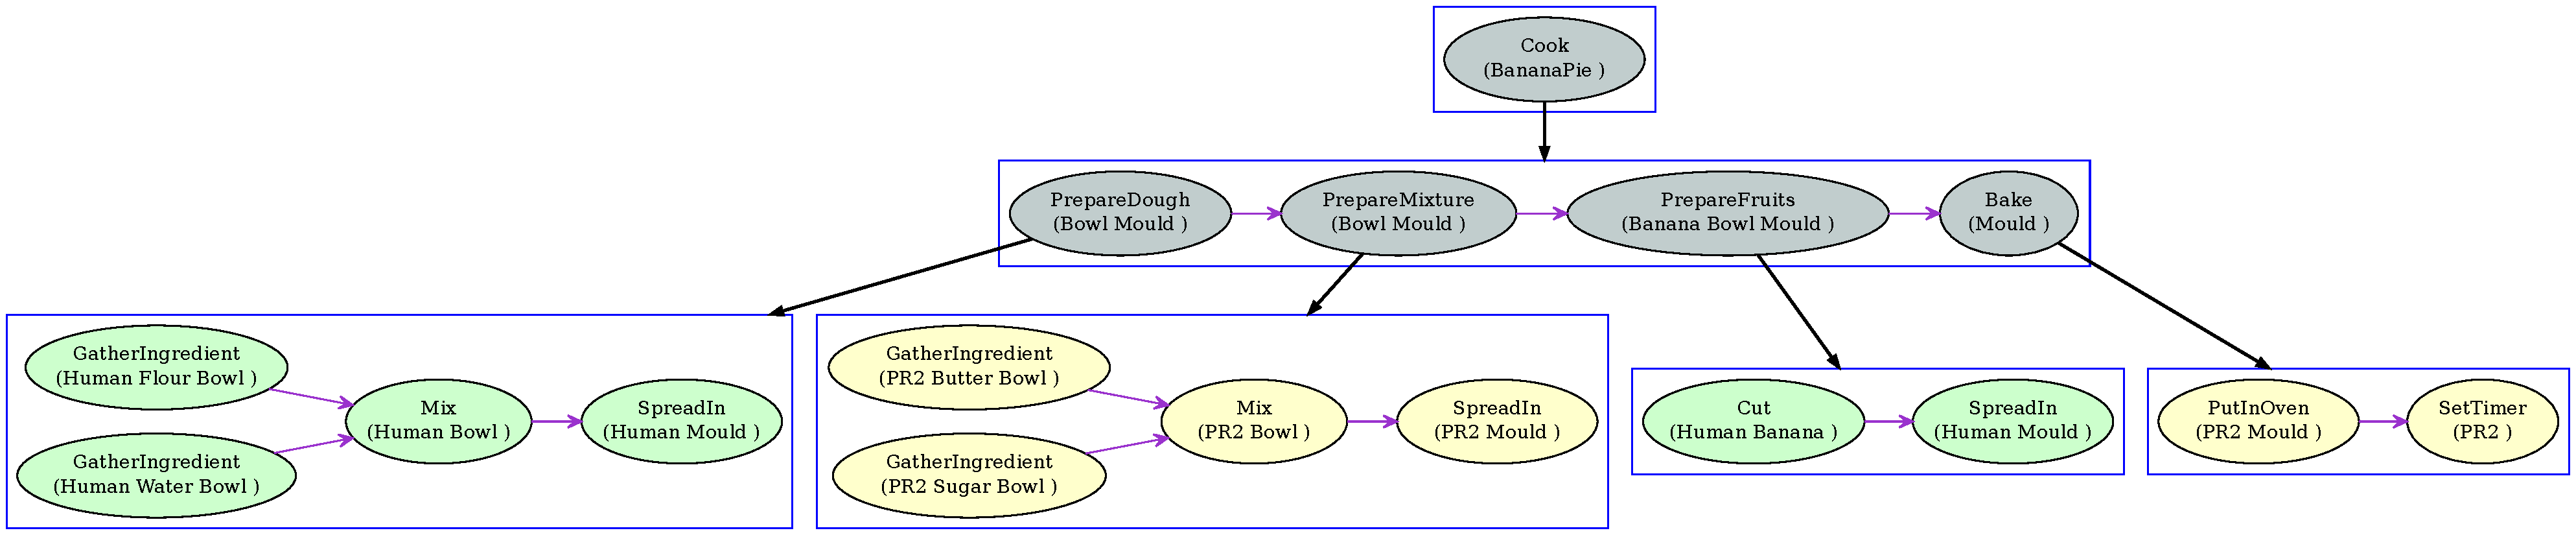
\includegraphics[width=0.99\textwidth]{img/teacher/bananaPie.pdf}
 \end{tabular}
   \vspace{-8pt}
 \caption{Shared plan and associated HTN generated to collaboratively make a banana pie.}
 \label{fig:teacher_results-bananaPlan}
   \vspace{-22pt}
 \end{figure*}
 

\begin{enumerate}
\item The human will prepare the dough, kneading it and putting it in the mould.
\item The robot will prepare a mixture with butter and sugar, putting the ingredients in the mould.
\item The human will then prepare the required fruits, cutting them and adding them to the mixture..
\item Then, the human will prepare the dough for the top of the pie.
\item Finally, the robot will bake the pie, by putting it into the oven and setting a timer.
\end{enumerate} 

After completing task 1, the human's knowledge on how to prepare the dough will be improved. Consequently, during the execution of task 4, the robot will ask the user if he needs help to prepare the second dough. We imagine he answers ``no". The robot does not explain the task  and the system will upgrade the human's knowledge level for the \textit{PrepareDough} task to  \textit{intermediate}, after he completes its execution. The human's knowledge of task 3, \textit{PrepareFruit}, will be represented as \textit{human1 PrepareFruits [fruit] VALUE}. We consider the parameter of this task as \textit{class-link} , since the process will be the same for any fruit (cutting and putting in the mould). This way we use, as parameter, the class \textit{fruit} instead of the actual instances used in the task, \textit{apple} or \textit{banana}.

After cooking the first pie, the robot generates a plan to cook the banana pie. This time, we set the environment in order to allow  each agent to perform all the tasks. Preparing a banana pie is a similar process to the apple pie. The parameters will, of course, be different, involving bananas and not apple. Also, the banana pie does not have a second dough on its top, and it has a different baking time from the apple pie. The plan generated is presented in figure \ref{fig:teacher_results-bananaPlan}. We can observe that the planner took into account the experience acquired by the human when preparing the apple pie, by assigning him the tasks (\textit{PrepareDough} and \textit{PrepareFruits}). During execution, since the user has an \textit{intermediate} knowledge level on \textit{PrepareDough}, the robot will not explain it. When the human is about to execute \textit{PrepareFruits}, the robot will propose to explain him the task, since he only performed it once, and has a \textit{beginner} knowledge level on it.


\section{User Study}
We have conducted a comparative user study in order to have a first evaluation of our system's adaptability by users. Two groups of users were asked to participate in the two-pies scenario. The first group interacted with a simulated robot equipped with a basic system (BS). BS has the same behavior as our system, excluding the agent knowledge awareness mechanisms. The second group interacted with another system, which we will call knowledge system (KS), and exhibits similar characterstics to the presented system.

The hypothesis of our study is that, on average, users will express a preference on KS over BS. More formally, we set our null $H_0$ and alternative $H_A$ hypotheses as follows:
\begin{itemize}
\item $H_0$: $\mu_{KS}-\mu_{BS}=0$ 
\item $H_A$: $\mu_{KS}-\mu_{BS} \neq 0$  
\end{itemize}


In both system, we will use the same task allocation presented in section~\ref{sec:teacher_results-scenario} to achieve the apple pie cooking example. Once the agents have cooked the first dessert, the robot generates a plan to cook the banana pie. 
In KS,  the robot favors a task distribution for the banana pie where the human performs tasks he has already executed in the previous scenario (preparing dough and fruits).
In BS, we imagine that the robot could allocate the tasks differently, asking the human to prepare the mixture instead of the dough.

Two groups of 19 participants, from 18 to 60, interacted with each system in an online user study\footnote{User study for KS http://goo.gl/forms/qvbtu4vcFW, and BS http://goo.gl/forms/ZSvGcCi5le}, where we presented pictures of the task state and recordings of the robot's speech, in French, for each step of the interaction (as shown in figure~\ref{fig:teacher_results-user_study}).
At some steps, the user could choose the action to perform, allowing him to execute a wrong action, leading to a replan from the robot. For simplicity, the replan just corrected the wrong action, before resuming the previous plan. 
At the end of the simulated interaction, we have asked the same questions to both groups, concerning the adaptability of the system and the robot partner itself. 
The users gave marks along a Likert scale from one (disagree) to five (agree) to express their agreement with several statements (as shown in figure \ref{fig:teacher_results-user_study}).

\begin{figure}[ht!]
 \centering
 \begin{tabular}{cc}
  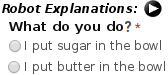
\includegraphics[width=0.24\textwidth]{img/teacher/ustudy9.png} &
  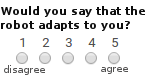
\includegraphics[width=0.19\textwidth]{img/teacher/ustudy11.png}
 \end{tabular} 
 \caption[User studies on plan adaptation]{\textit{Left}: The user listens to recorded robot explanation and chooses the action to take. \textit{Right}: At the end, the user evaluates the interaction using a Likert scale.}
 \label{fig:teacher_results-user_study}
 \end{figure}

\section{Results}

We collected the answers from each form, and computed the mean, along with the standard deviation and p-value to evaluate the system. The p-value was computed using a t-distribution with 18 degrees of freedom and evaluated using a significance value $\alpha=0.05$.
%We compare below the results for each system. 
Figure~\ref{fig:teacher_results-results} summarizes the results. Comparing users' answers, we can see that users appreciated the capacity of the system to explain the plan while adapting to their knowledge, with a mean of 3.74 for KS against 2.05 for BS. The users interacting with KS globally noticed that the task distribution took their knowledge into account, by giving a mean rating of 3.42 for KS and 2.58 for BS. The last question concerned the freedom to choose how to perform the task. In this case, the calculated mean was 2.58 for KS and 1.89 for BS. In all these cases, the p-value was lower than the $\alpha$. 

With KS, the users attributed a mean of 3.11 for the global adaptability of the system against 1.89 for the basic one.
We also asked how the robot partner was perceived. While in KS the robot is not perceived as more verbose (2.53 for KS against 2.47 for BS), people found the interaction slightly more natural (2.74 against 2.42) and the robot appeared smarter (2.79 against 2.26). Even if these last two results look favorable, since their p-value is higher than $\alpha$  we do not have enough evidence to prove a difference between the two systems. We believe that other aspects might have been taken into account by the users, such as the speech itself, which conditioned their perception on the naturalness of the interaction. Improving the robot's verbalization process with a synonym dictionary could be a first step to get more significant results.



 \begin{figure}[ht!]
 \centering
 \begin{tabular}{cc}
  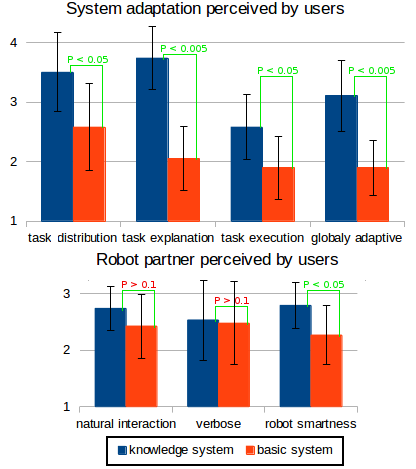
\includegraphics[width=0.45\textwidth]{img/teacher/respvalue3.png}
 \end{tabular}
 \caption[Average users' rating of the interaction on several criteria]{Average users' rating of the interaction on several criteria. Blue for KS and red for BS.}
 \label{fig:teacher_results-results}
 \end{figure}

This study sheds light on how users were able to perceive the robot adaptation to their knowledge concerning task distribution, task explanation and monitoring. In addition, the robot partner was perceived as smarter and the interaction seemed a bit more natural to the users. However, these first results need to be confirmed with study on a larger population. Also, as the scenario was simulated, results on a real robot might differ.
In both studies, we asked the participants how the system could be improved. Several users suggested they would like to be able to choose which action to perform, showing the importance of negotiation. A user suggested he would like to be informed about the progress of the task from time to time. Other comments concerned suggestions about the robot's speech capacities, like its voice voice, its intonation, and the chosen words. These aspects were not the aim of our  experiment but are indeed an important part of the interaction process. 
 



% % Chapter Template

\chapter{Introduction} % Main chapter title

\label{chapter-introduction} % Change X to a consecutive number; for referencing this chapter elsewhere, use \ref{ChapterX}

\lhead{Chapter . \emph{Introduction}} % Change X to a consecutive number; this is for the header on each page - perhaps a shortened title

%----------------------------------------------------------------------------------------
%	SECTION 1
%----------------------------------------------------------------------------------------

In the current days robots are starting to be introduced in our lives more and more, and we can expect that, in the next years, they will complete the transition from mechanic tools, used mostly in industries, to true partners and companions. There is an increasing interest in studying how robots should behave in environments inhabited by humans, and in some works robots have been deployed in crowded and dynamic environments, like airports and museums.

Human-Robot cooperation poses a multitude of problems. Imagine a mobile robot working in a warehouse, carrying and sorting crates in different locations. Already, we are presented with quite a complex problem, where the robot needs to have a good representation of the world (i.e. position of the crates, obstacles, layout of the warehouse), to create plans to reach the goal (which crates to move, where to bring them, which paths to follow), and to have sufficient motion and manipulation skills to achieve them. If humans are present in the environment, they should be represented and considered by the robot in its plans and actions.  Modeling humans as simple moving obstacles might not be enough if we consider issues of trust, legibility, and acceptability. The robot should respect a number of social rules in the presence of humans, like maintaining a socially acceptable distance, whenever possible, from them, and approaching them from a visible positions.

The problem becomes even more complex when robots and humans need to cooperate to solve a goal, for example by sorting together the crates, or even by sharing the load of heavy objects. To understand  how to approach this problem we can observe how humans cooperate with themselves. Psychological and philosofical research \cite{pacherie2012phenomenology} characterizes the execution of cooperative actions as 'joint actions'. Sebanz et al. \cite{sebanz2006joint} have proposed that the execution of a joint action depends on three different abilities: sharing representations, predicting actions, and integrating predicted effects of own and other's actions. These abilities can be achieved by the combination of different mechanisms:
\begin{itemize}
\item Joint Attention. The ability to direct a partner's attention, in order to create a shared representation of objects and events. Humans use a large number of social cues, like gaze direction or pointing gestures, to indicate what is currently under observation. This mechanism helps filling important gaps in the knowledge of a partner, and points to the importance of understanding what others know and perceive.
\item Action Observation: observing other partners' actions is crucial in understanding what are their goals. Studies have shown that observing a person performing an action produces a motor resonance, which increases with the observer's level of expertise in the action. Understanding what others are doing allows to predict the outcomes of their activities, and even their next movements.
\item Task Sharing: humans are able to predict, in some circumstances, what others will do  even without direct observation. A notable example is a well trained sport team, which is able to act like a single entity, coordinating seamlessly. This ability suggests that humans possess a shared representation of tasks, which include actions that should be performed by each partner of the team.
\item Action Coordination: predicting actions is not enough. Humans also need to choose a complementary action, and adjusting its parameters, like the exact moment and place where it should be performed, to partners. 
\end{itemize}

It seems that robots need to have an equivalent of these mechanism, in order to cooperate in a natural and acceptable way with humans. Is this enough to include robots in our lives? Unfortunately, we just scratched the surface of the problem. While these areas are already very complex, and not completely understood, humans possess other skills, that should be translated to robots. For example, when a robot's behavior shows a degree of intelligence, humans usually try to have a conversation with it, which can lead to frustation, or often disbelief in the actual capacities of the robot. Issues such as dialogue, representation and refinement of knowledge are very complex and will be a direct focus of this work.

The goal of this thesis is, instead, to provide a framework to allow a robot to work in social environments and execute joint actions with humans in a natural way. We built our system using psychology as an inspiration, without trying to replicate accurately human mechanism, an area of work studied in cognitive systems. 

There are still not many robotic architecture that take humans into account at all levels, from planifications to execution. We will review some examples:
\begin{itemize} 
\item \cite{trafton2013act} presents ACT-R/E, a cognitive architecture, based
on the ACT-R architecture, used for human robot interaction tasks. The
architecture aims at simulating how humans think, perceive and act in
the world. ACT-R/E has being tested in different scenarios, such as
theory of mind and hide and seek, to show its capacity of modeling
human behaviors and tought.
\item In \cite{Fong_2006} the authors present  HRI/OS, an agent-based system
that allows humans and robots to work in teams. The system is able to
produce and schedule tasks to different agents, based on their capacities,
and allows the agents to interact mostly in a parallel and independent way, with
loose coordination between them. Cooperation  mainly
takes place when one agent asks for help while
dealing with a situation. In this case the HRI/OS will
look for the best agent to help, based on their availability and capacities.

\item In \cite{clodic2009shary} the authors build SHARY, a supervision
system for human robot interaction, tested in domestic environments to
perform tasks such as serving a drink to a person. Our system is an
evolution of Shary which includes new aspects, like spatial
reasoning and modeling of joint actions.
\end{itemize}

\section{Contributions}

The main contributions of this work are the following:
\begin{itemize}
\item Building a supervision system for human robot interaction, integrating novel algorithms developed in this work with existing, components.
\item Developing a novel algorithm to infer human goals and intentions.
\item Developing a novel probabilistic planning algorithm for multiple agent.
\end{itemize}

\section{System overview}
\label{intro-system_overview}
%TODO: add urls, PR2, GAZEBO, ROS, SPENCER, GTP, Move_Base, Moveit
The supervision system was developed with the following goals:
\begin{itemize}
\item Flexibility. The system is able to work in different scenarios, environments, and different robots.
\item Extendibility. The system can be easily extendable by adding or substituting modules, to introduce different capacities, without having an impact on existing components.
\item Human-Awareness. The system supports human in all its layers. Human belief management, multi-agent planning, human-aware motion and execution, and simple forms of direct interaction are explicitly included in its components.
\end{itemize}

To achieve these goals we use the well-known ROS framework\footnote{http://www.ros.org/}, which naturally supports different robots and modules.The system has been implemented and tested in simulation, using the GAZEBO simulator\footnote{http://gazebosim.org/}, and on two different robots, the PR2 by Willow Garage\footnote{https://www.willowgarage.com/pages/pr2/overview}, and the SPENCER robot\footnote{http://www.spencer.eu/}, developed in an european research project. 

The supervision system is composed by the following layers, as shown in figure \ref{fig:intro-system_architecture}:
\begin{itemize}
\item Situation Assessment. This layer produces symbolic information, using geometrical and temporal reasoning, starting from perception data. Using Situation Assessment, the robot is able to compute information like the reachability of objects, which actions have been performed by humans, and the spatial relationships (distance, orientation, and their variations) between humans and the robot. This layer also includes a Database, which collects collects all the symbolic information produced by the system. The Database is able to represent the knowledge of different agents, as viewed by the robot. Using this feature, the robot can represent, for example, the fact that a human does not know the location of an object, or that he has wrong information about its location.
\item Goal Management. This layer manages the different goals of the robot. Goals can be directly received from exernal inputs, like a human or a terminal, or generated by the robot starting from information present in the Database. For example, after deducing that the human is looking for his glasses in the Situation Assessment Layer, the Goal Management Layer can create a goal to fetch them. 
\item Plan Production and Management. This layer is charged with producing and managing plans to achieve the current goal. The system supports multi-agent plans, and so the robot will monitor other agents' action, to check if they conform to the shared-plan, and interact with the Execution Manager layer to execute the robot's actions. Plans can be managed in three different modalities: robot leader, human leader, and equal partners. Human-Awareness is supported by adapting  production, explanation, and management of plans to the level of experience on the task of the robot's partners. Additionally, this layer supports a simple form of plan negotiation, which allows humans to express preference in the allocation of tasks.
\item Execution Management. This layer handles the execution of the robot's actions, including joint actions shared with other agents. Human safety and robustness are achieved by stopping and resuming operations  when unexpected or dangerous situations arise, like a human moving into the operative area of the robot.
\end{itemize}

 \begin{figure}[h!]
	\centering
	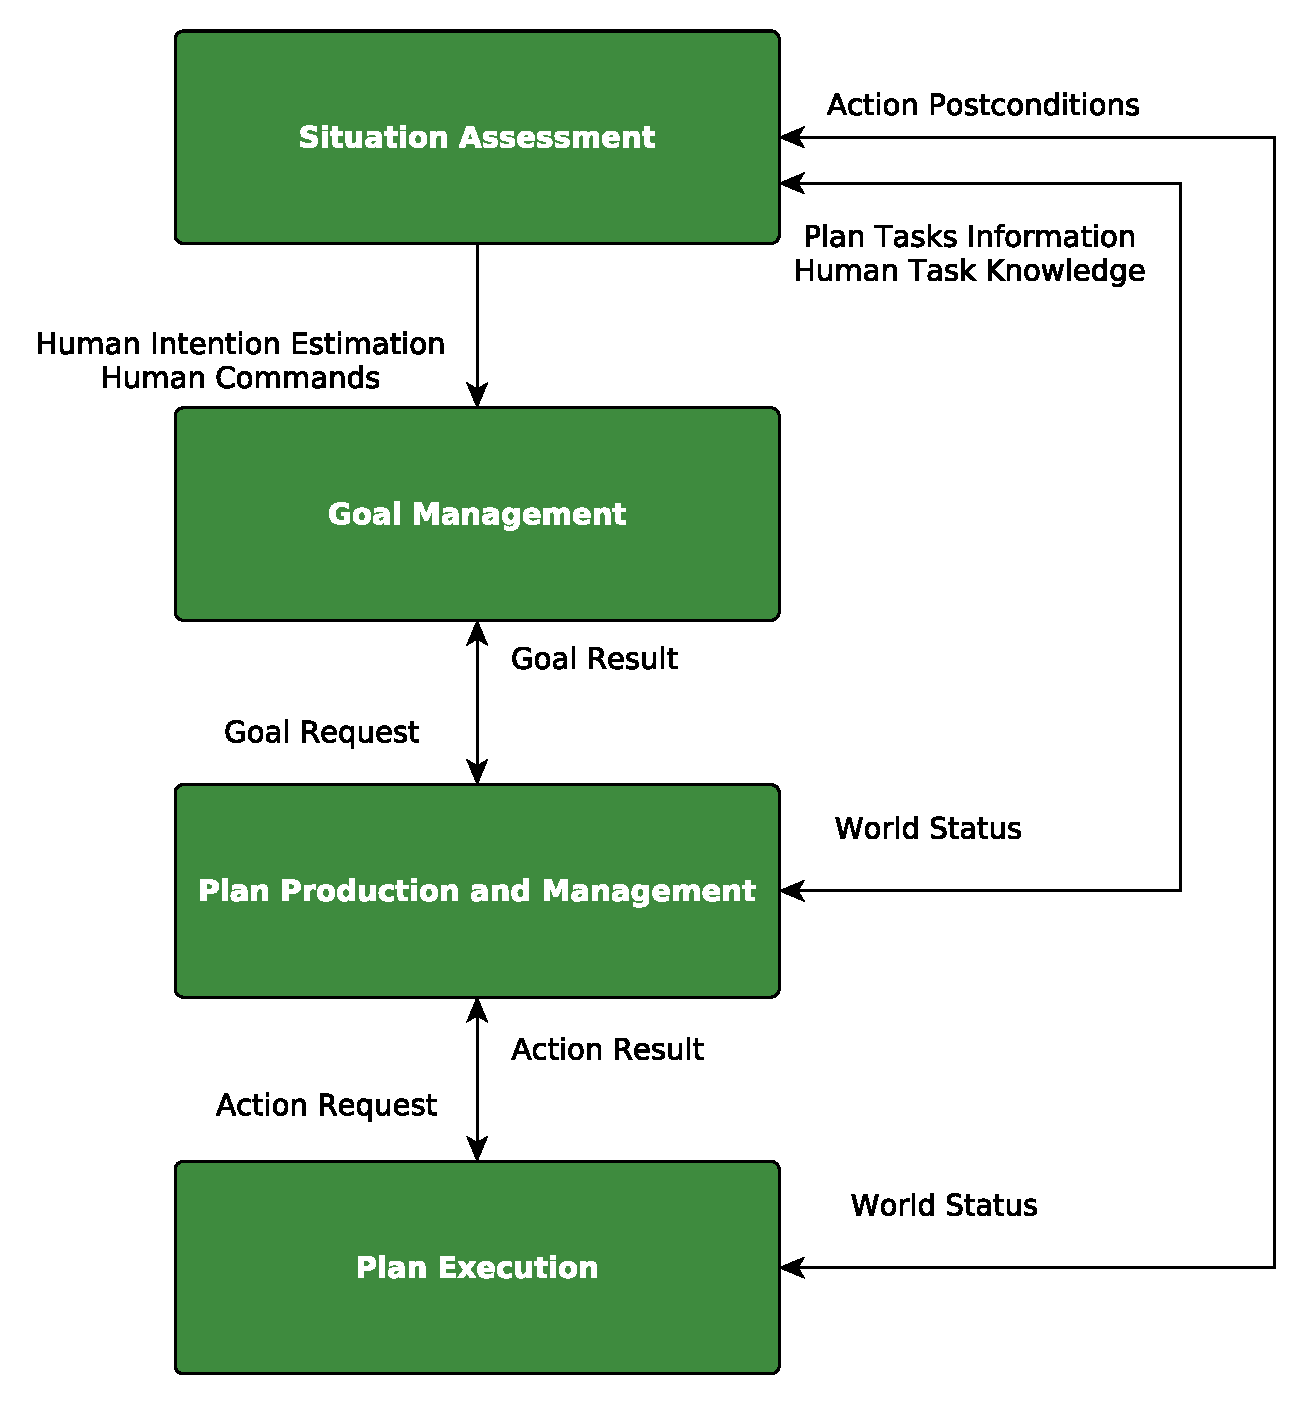
\includegraphics[scale=0.45]{img/intro/system_architecture.pdf}
	\caption[System architecture]{This picture shows the different layers of the system.}
	\label{fig:intro-system_architecture}
\end{figure}

The system also easily interface with different modules, which can be changed depending on the current needs:
\begin{itemize}
\item Task Planner. The Plan Production and Management layer provides an interface for different planners. New planners can be introduced by creating a bridge that respects the interface provided by the provided interface.
\item Motion Planners and Executors. The Execution Management layers is interfaced with a set of motion planners and an executor to accomplish the robot's movements and actions. New modules can be introduced by respecting the interface used in the layer.
\end{itemize}

\section{Organization of the Thesis}
This thesis is organized in several chapters. \ref{chapter:situation_assessment} discusses the Situation Assessment Layer, introducing its functionalities and a study to assess a part of its capacities. \ref{chapter:goal_management} shows how our system is able to receive, generate, and manage goals. \ref{chapter:plan_management} analyzes the capacity of our system to produce and manage plans. We discuss two different planners introduced in our system, and the process to explain, negotiate, and adapt plans to users. Finally, we present several plan management algorithms, with different characteristics. \ref{chapter:plan_execution} shows how our system is able to support action executed single-handedly by the robot, as well as our framework to execute joint actions with a human partner. \ref{chapter:case_study} presents two different applications where we used our system: a domestic robot helper and an airport guide. Finally, "introduce conclusion", concludes this work, discussing several possible future extensions. 

\section{Published Works}
\begin{itemize}
\item Milliez, Grégoire, et al. ``Simulating human-robot interactions for dialogue strategy learning." Simulation, Modeling, and Programming for Autonomous Robots. Springer International Publishing, 2014. 62-73.
\item Triebel, Rudolph, et al. ``SPENCER: A socially aware service robot for passenger guidance and help in busy airports.", 2015.
\item Fiore, Michelangelo, et al. ``An Adaptive and Proactive Human-Aware Robot Guide." Social Robotics. Springer International Publishing, 2015. 194-203.
\item Fiore Michelangelo, et al. ``On planning and task achievement modalities for human-robot collaboration." Experimental Robotics. Springer International Publishing, 2016.
\item Milliez, Grégoire, et al. ``Using human knowledge awareness to adapt collaborative plan generation, explanation and monitoring." The Eleventh ACM/IEEE International Conference on Human Robot Interation. IEEE Press, 2016.
\item Devin, Sandra et al. ``Some essential skills and their combination in an architecture for a cognitive and interactive" robot arXiv preprint arXiv:1603.00583, 2016
\item Caccavale, Riccardo, et al. ``Attentional Supervision of Human-Robot Collaborative Plans." The IEEE International Symposium on Robot and Human Interactive Communication (RO-MAN), 2016.
\end{itemize}
% \part{The Robot Teacher} % Main chapter title

\label{part:robot_teacher} % Change X to a consecutive number; for referencing this chapter elsewhere, use \ref{ChapterX}

\lhead{Part 1. \emph{The Robot Teacher}} % Change X to a consecutive number; this is for the header on each page - perhaps a


In any application that is not entirely composed by repetitive, precomputed actions, robots need reasoning skills, which severely depend on the quality of the representation of the current environment. This representation can be more or less complex, depending on the application. 

Imagine, for example, a robot whose task is cleaning the floor of a room. In the simplest case, this robot would only be provided with an elementary set of sensors. Without the capacity to understand which areas actually need cleaning, this robot could only move through the room, randomly or with some strategy, achieving the task in a longer amount of time than what would actually be needed. 

% In a fairly simple case, this robot would rely on a map of the room and a set of lasers, or bumper sensors, to detect obstacles. 

Now, imagine a household robot that needs to actively help a family that lives in an apartment, by fetching objects, providing information, and helping to accomplish various tasks. Let us imagine that one of the members of the family, Greg, is moving in the living room, searching around, while exclaming `Where are my glasses?'. In the ideal situation, our robot would try to help Greg, by giving him information such as `They are on the table to your right', or even by fetching them for him. 

Clearly, in this scenario, the robot needs deeper reasoning skills. It needs to understand that the user is looking for its glasses, to link them to their actual physical location, to compute the spatial relationship between the table and the glasses, and to provide information in a natural way. In fact, if the robot would tell Greg that the glasses are in the position $(3.2, 5.0 , 1.3)$, Greg would very likely be very perplexed. A more natural way would be to inform Greg that his glasses are on a table, whose location is pointed taking into account Greg's position.

In this case, having sophisticated sensors is, of course, important but not sufficient. The robot needs also to \textit{reason} on the sensor's data in order to produce meaningful information. For example: laser points and camera images need to be integrated to recognize objects and humans; spatial relationships  (e.g. the glasses are on the table) have to be properly modeled; actions performed by humans, and their effects on the environment, need to be recognized; and so on. 

The process of reasoning on data to produce symbolic information is called \textit{situation assessment}. Endsley explained in \cite{endsley1995toward} that this process is deeply linked to the quality of  decions of the robot.

While in many applications robots can benefit from a situation assessment component, being able to perform complex reasoning on data is particularly important in HRI. If the robot is able to take better decisions (i.e.  efficient, safe, socially acceptable, natural) than it will be perceived in a more positive manner by humans. 




                 % Chapter Template

\chapter{Situation Assessment} % Main chapter title

\label{chap-situation_assessment} % Change X to a consecutive number; for referencing this chapter elsewhere, use \ref{ChapterX}

\lhead{Chapter . \emph{Situation Assessment}} % Change X to a consecutive number; this is for the header on each page - perhaps a shortened title

In this chapter we introduce the Situation Assessment capacities of our system. 

%TODO: Citations on Toaster. Look and add other possible citations. Cite everything. Everything!
\section{Introduction}
\label{sec:situation_assessment-intro}
\subsection{What is Situation Assessment?}
%Motivation
In any application that is not entirely composed by repetitive, precomputed, actions, robots need to possess adeguate reasoning skills, which severely depend on the quality of the representation of their environment. This representation can be more or less complex, depending on the application. Imagine, for example, a robot that needs to clean the floor of a room. For a fairly simple case, this robot would rely on a map of the room and set of lasers, or bumper sensors, to detect and obstacles. Now, imagine a household robot that needs to actively help a family that lives in an apartment, by fetching objects, providing information, and helping accomplish various tasks. Clearly, in this situation, the robot needs a deeper degree of reasoning on sensor data: laser points and camera images need to be integrated to recognize objects and humans; spatial relationships  (e.g. the cup is on the table, the human has the cup) need to be properly modeled; actions performed by humans, and their effects on the environment, need to be recognized; and so on. 

In this situation, there is a need for a process which performs different kinds of reasoning on perceptual data, and produces information that can be used by the rest of the system. This process is called situation assessment, and is deeply linked to the quality of the decisions of the robot, as explained by Endsley in \cite{endsley1995toward}. 


%what are people doing with situation assessment and belief management
Situation assessment components have been designed by different authors, but they are usually developed for specifc applications, like in \cite{Chella2010,Kluge01situationassessment}. In \cite{beetz2015robosherlock}, instead, the authors present ROBOSHERLOCK, an opersource framework that can be used to implement perception systems. Among its features, ROBOSHERLOCK supports logical queries about the world state, and so supporting task-driven situation assessment. 

\subsection{Theory of Mind}
An important part of Situation Assessment is representing other agents in the environment, not as simple obstacles, but as acting entities, with different beliefs on the state of the world, and with the capacity to affect the environment. 

Theory of Mind \cite{premack1978does} is a skill used to reason about humans' beliefs and thoughts, and how they affect actions. An ability linked to this concept is perspective taking, which is widely studied in developmental literature.  Flavell in \cite{flavell1977development} describes two levels of perspective taking: 
1) perceptual perspective taking,  the capacity to understand that other people see the world differently ~\cite{Tversky1999}; and 2) conceptual perspective taking, the capacity to attribute thoughts and feelings to other people ~\cite{Baron1985}. Studies on individuals that don't possess the required mechanisms to perform perspective taking, like young children \cite{frick2014picturing}, have put into light the difficulties these people have to accomplish everyday social relationships and confirmed the importance of this ability.

Previous works in robotics have shown that enhancing the robot's perspective taking abilities improves its reasoning capabilities, leading to more appropriate and efficient task planning and interaction strategies \cite{Trafton2005,ros2010one}. \cite{breazeal2006} showed that perspective taking can even enhance learning by imitation processes, allowing the viewer to learn a task from "flawed" demonstration, which may be correct from the teacher's point of view but are actually ambiguous. 

An important study linked to conceptual perspective taking is the 'divergent belief task'.  Formulated in~\cite{wimmer1983}, this kind of task requires the ability to recognize that others can have beliefs about the world that differ from the observable reality. ~\cite{BreazealGB09} proposed one of the first human-robot implementations, resulting in more advanced goal recognition skills. 

Not many frameworks throughly model different agent's beliefs.  Scheutz \cite{scheutz2013computational}) studied this problem, developing a computation model to represent agent's mental states. The work is oriented in particular toward communication problems and not geometrical and spatial perspective taking issues.

\subsection{Intention Recognition}
%TODO: here in particular we need something for action recognition
Another crucial skill of a robot that interacts with human is recognizing others' actions and goals. Recognizing others' goals is directly linked to modeling humans' beliefs, since, as explained by \cite{byom2013theory} "as humans, we generally believe that others act in ways that are consistent with their beliefs and goals". In psychology \cite{bruner1981} and philosophy \cite{bratman1984} literature, an intention as the wish and will to achieve a goal. Intentions memerge from contextual causes (motivations) and are present the goal is achieved or abandoned, pushing agents to undertake actions leading to that goal.

The recognition of human activities is an important topic in computer science research, which can be studied at different levels. Anticipating human actions and movements allows the robot to adapt its behavior and proactively help humans, as studied in \cite{koppula2013anticipating}. An interesting idea is using the robot's own internal models in order to recognize actions and predict user intents, as shown by the \textit{HAMMER} system in \cite{demiris2007prediction}. Sequences of actions can be linked to plans, a well-known topic called plan recognition. Several approaches have been studied in this domain using, for example, classical planning \cite{ramirez2009plan}, probabilistic \cite{bui2003general} or logic techniques \cite{singla2011abductive}.  In \cite{talamadupula2014coordination}, the authors use classical planning, with an efficient replanning strategy, in order to infer user's intentions. The system has been implemented on a PR2 robot and tested on a collaborative scenario. \cite{breazeal2009embodied} presents an architecture in which the robot is able to use its own schemas and models to infer human actions and goals, and to proactively help him achieve them. Shared plans are not explicitly represented in the system, and the robot helps the human by mapping the inferred goal information in its own beliefs, and choosing appropriate action

Two approaches that can be used for intention estimation are Interactive Partially Observed Markov Decision Processes (I-POMDP) and Inverse Learning. I-POMDP  \cite{gmytrasiewicz2004interactive} offer a rich framework that extends Partially Observed Markov Decision Processes (POMDP) in a multi-agent setting. Inference in these models can be extremely complex, but there have been attempts at solving this issue, like in \cite{doshi2009monte,hoang2013interactive}. 

Inverse Reinforcement Learning \cite{ng2000algorithms} formulates the problem of computing an unknown reward function of an agent after observing his behavior. This strategy has been applied, with Bayesian Networks (BN), in \cite{Nagai2015}, in order to learn the mental model of another agent, and choose appropriate actions for a relationship building task. A linked approach is inverted planning, which has been applied in a bayesian framework in \cite{baker2009action}  for human action understanding.

Contextual information can be used to further disambiguate complex situations. \cite{Liu2014} shows a system using BNs to understand users' intentions with an emphasis on contextual information.

It is very important to consider humans' beliefs when estimating their intentions. In a dynamic environment, agents can execute actions, modifying the state of the world without other agents being able to perceive the changes. Let us imagine a scenario. Bob comes back home from work and would like to relax while reading. He lays down on a sofa with a book, and reaches to a nearby table to grab his glasses. He does not know that his wife, during the day, moved the glasses to another room. If we would ignore Bob's beliefs on the world (i.e. he does not know that the glasses are not on the table) we could infer that, for example, Bob would like a drink while he is sitting on the sofa, or the tv remote controller. If, instead, we would know that Bob thinks his glasses are on the table (and we would use other contextual information perhaps, like Bob's habitudes) we would be able to correctly infer Bob's current intention, that is, taking his glasses, and warn him that they are not there, perhaps even fetching them for him. In robotics, an interesting framework that considers this issue is the Bayesian Theory of Mind \cite{baker2014modeling}, used to represent the inference process of an observer looking at another agent's behaviors, with POMDPs and Dynamic Bayesian Networks (DBNs).


\subsection{Dialogue}
Dialogue is a very important part of situation assessment. Agents often communicate, while executing a task together, or even when working independently, to clarify ambiguities and obtain missing information. While we will not present a specific dialogue component in this work, we have used our system in \cite{Ferreira2015}, where our belief management component and a situated dialogue system were implemented in a simulator. This model was compared with a basic system (without belief awareness) in a study with 60 interactions, in a simulated environment. We successfully showed that the dialogue management system significantly improves its efficiency, reducing the number of dialogue turns in the interaction, and its accuracy, with a higher success rate when a divergent belief situation appears.

\section{System Overview}
\label{sec:situation_assessment-overview}

In our architecture, we built a Situation Assessment layer, which is able to:
\begin{itemize}
\item  Detect and track entities.
\item  Process sensor data in order to produce symbolic information.
\item  Maintain a belief model for each agent.
\item  Infer human actions and intentions. Our system is able to perform this estimation by taking into account the current belief of humans on the world state. 
\end{itemize} 

This layer is composed by different elements, as shown in Fig. \ref{fig:situation_assessment-situation_assessment_overview}.
\begin{itemize}
\item Sensor Data. Data produced by different possible sensors (e.g. lasers, camera, etc.)
\item Entity Detection. Different components detect and track humans and objects in the environment.
\item Human Inputs. Users can communicate with the robot by using a tablet application.
\item Human Interface. User inputs from the tablet are elaborated into commands, to introduced in the Database.
\item Geometrical Reasoning. Symbolic facts are produced starting from perceptual data.
\item Belief Management. The system maintains a mental model of each agent.
\item Intention and Action Recognition. Human actions and intentions are inferred based information provided by the Geometrical Reasoning and on the belief models of the agents.
\item Database. The database stores symbolic facts produced by the system.
\end{itemize}


 \begin{figure}[h!]
	\centering
	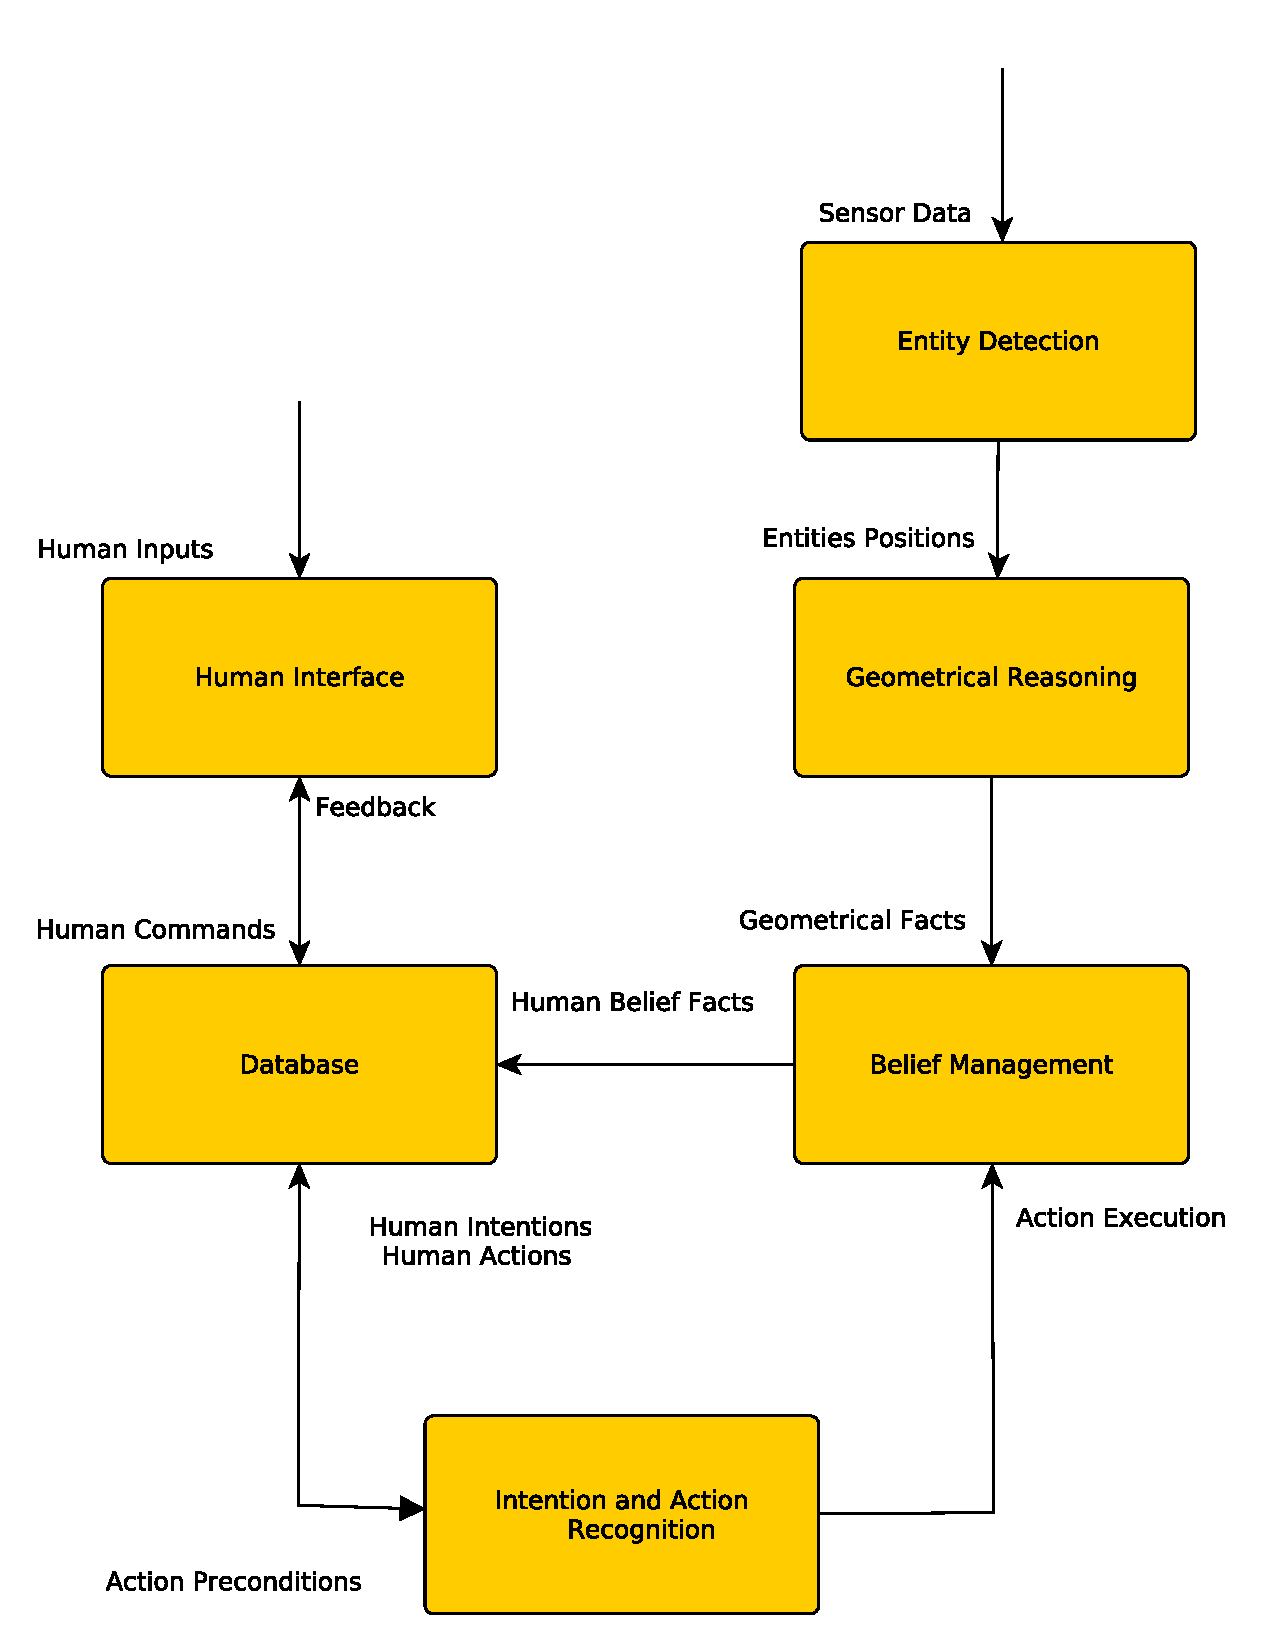
\includegraphics[scale=0.45]{img/situation_assessment/situation_assessment_overview}
	\caption{Overview of the different modules composing the Situation Assessment Layer}
	\label{fig:situation_assessment-situation_assessment_overview}
\end{figure}


In addition, the system possesses a description of the world, with a definition of all the elements known to the robot, like objects and agents, possible actions, possible intentions, intentions, etc. 
Symbolic facts are constantly produced starting from the sensor data and from the position of entities, and then the Belief Manager will update and maintain the belief model of each agent. The belief model of humans and of the robot will be used by the Intention and Action Recognition modules to infer the most likely intentions and actions performed. All these information are introduced in the Database, and can be read by other components. For example, the Goal Manager can choose a goal based on human commands or on an estimation of its intention. In a similar way, the Action Execution modules will read the Database in order to obtain the state of the world, to check action preconditions.  

Our situation assessment layer was presented in \cite{Milliez2014}, where it was used to pass the Sally and Anne test~\cite{Baron1985} on a robotic platform. The intention and action recognition capacity was introduced in \cite{devin2016some}.

\section{Object and Human Detection}
In our system, we chose to simplify perception issues, focusing on reasoning aspects. We associate a unique tag to every object that is interesting in a particular scenario.  When the robot observes a tag using a camera, it detects the corresponding object using a tag-matching algorithm.
Regarding humans, we use a motion capture software to identify and track agents moving in the environment. Using different tags, we can track the head, shoulders, and right arm of a human. Our situation assessment component has also been tested using a laser and RGB based detector in the SPENCER european project \footnote{http://www.spencer.eu/}.

\section{Human-Robot Communication}
Similarly, communication between the human and the robot is limited, in our system. Humans can give commands to the robot by using a tablet application, where they can manage the robot goals, by adding a new goal, canceling a previous one, or pausing the robot. The robot is able to provide simple verbal output by using a text-to-speech component. The robot is not able to perform real dialogues with the human but it can adapt its speech to the current tasks and scenarios, by explaining plans, informing the human if it has a problem, verbalizing its current actions, and so on. This feature will be explained fully in chapter \ref{chap-plan production and management}. 

\section{World Model and Geometrical Reasoning}
\label{sec:situation_assessment-situation_assessment}
The first step in estimating human intentions is reasoning about the environment and the belief of humans. Our world is composed by agents, the robot and humans; by objects; and by areas, which are bounded regions in the environment with semantic meaning, e.g. living room, kitchen. To be more generic, we will sometimes use the word \textit{entity} to refer to an agent, an agent's joint or an object. We can assign properties, to entities and areas to represent different information, e.g. 
an agent can be in a specific area, a box can be opened and can contain objects, a bottle can contain liquids, a mug can be hot. The $subject$ of a property is the name of the primary entity linked to it (e.g. bob, mug). 
 We divide properties in two classes: 
\begin{itemize}
\item fully observable:  can be seen by any present agent looking at the linked entity or area, e.g. the box is open
\item partially observable: can be observed by present agents only in specific situations, represented as rules linked to the object and the property, e.g. an agent can see that a box contains items only when it is open, an agent can detect that the mug is hot only when he touches it.
\end{itemize}

Using its perception abilities the robot can build a representation of the environment, starting with entities' positions. Using geometrical reasoning we can compute spatial relationships between entities, e.g. the glasses are on the shelf, the human is moving toward the library, the glasses are reachable by the human, the bottle is visible for the human. These reasonings provide a base for the perspective taking abilities of the robot. 


\section{Belief Management}
\label{sec:situation_assessment-belief_management}
In our system, agents can have divergent representations of the world. To model this aspect, the information produced by perception, geometrical reasoning and inference, are collected by the robot in \textit{belief models}, built for itself and for each agent. A \textit{belief model} is a symbolic representation of the world state, as known by an agent. In a model, the world state is represented by properties and values. To represent the lack of knowledge of an agent, the value of a property can be \textit{unknown}.

We consider our world as a dynamic environment, where properties can change and actions can be performed.  We define an action as a tuple $(name, preconditions, target, postconditions)$. The $name$ of an action is a unique string that identifies it. The $preconditions$ are a list of properties that must be true in order to realize the action. In our system, an action is executed on a $target$, which can be a physical object, like a cup, but also an area of the environment, like a room. The $postconditions$ are the set of properties, and their values, affected by the action's execution.

Since we are interested on reasoning and not perceptual aspects, we use inference, as explained in Sec. \ref{sec:situation_assessment-intention_recognition}, in order to understand when a human has performed an action. Through the predefined $postconditions$ of actions we can also infer changes in object properties, e.g. the human opens a box, so the box is now open. 

We created a rule based framework in order to build the beliefs of each agent and update them when needed. Human belief models are updated using the perspective taking skills of the robot. When the robot detects the execution of an action in the world, it updates the belief model for itself and for every human that can perceive the action, adding the action's $postconditions$ to their models. When an action is not perceived by a human (e.g. the user was in an other room), his belief model will not be updated, as he is not aware of the changes that occurred.

However, when he comes back and looks at the environment, we assign him a new belief state following a set of rules, which we will now explain. We call $H$ the agent, $HB$ his belief model, and $RB$ the robot's belief model. We also create the following predicates: $obs(p)$ means that the instance of property $p$ is observable, $valid(p,x)$ means that the instance of property $p$ doesn't contradict the current perception data of agent $x$, $value(p,m)$ is the value of predicate $p$ in belief model $m$, and $vis(p,x)$ means that agent $x$ has visibility on the linked entities of property $p$. The rules for the $valid$ predicate will be different in each property. For example the property \textit{MUG isOn TABLE} won't be valid for agent Max if he can see that there is no mug on the table. For each property $p\in HB \cup RB$:
\begin{itemize}
\item if $p \in RB, \quad p\not\in HB,\quad obs(p),\quad vis(p,H) \rightarrow value(p,HB)=value(p,RB)$.
\item if $p \not \in RB,\quad p\in HB,\quad obs(p),\quad vis(p,H) \rightarrow remove\quad $p$ \quad from \quad HB$.
\item if $p\in RB,\quad p\in HB$ then:
	\begin{itemize}
      \item if $value(p,HB)\neq value(p,RB),\\ \quad obs(p),\quad vis(p,H) \rightarrow \\ value(p,HB)=value(p,RB)$.
      \item if $value(p,HB)\neq value(p,RB),\\ \quad !obs(p),\quad !valid(p,H) \rightarrow \\ value(p,HB)=\textit{unknown}$.
	\end{itemize}
\end{itemize}
The idea of this set of rules is updating an agent's mental belief model for a property only if it's observable, or if it's not observable and perception data contradicts the current value of the property (e.g. the mug was moved from the table to the kitchen while the agent was in another room: while the agent can not see where is the mug, he can see it is no longer on the table).



\section{Action and Intention Inference}
\label{sec:situation_assessment-intention_recognition}

In order to infer human intentions, we will provide the following information to the robot: a list of known contexts, a list of known intentions, a list of known actions, a set of observations of human actions, and a belief model of humans and of itself.

We propose, as central model used for intention estimation, a framework based on BNs. We call our implementation of BN an Intention Graph (IG).
An IG is linked to a specific agent, and composed by the following layers of nodes:
\begin{itemize}
\item Context Nodes: these nodes represent contextual information, modeled as boolean variables (e.g. HotDay, ColdDay).
\item Intention Nodes: these boolean nodes represent the set of possible intentions. Each intention can conditionally depend on several contexts.
\item Action Nodes. This is the set of human actions whose preconditions . Each of these nodes is conditionally dependent on all the intention nodes. 
\item Observation Nodes. We associate to each action a different set of observation nodes, that depend conditionally on the associated action node. 
\end{itemize}

In a typical usage, the robot will create, for each monitored human, an IG, formed by the Context and Intention Nodes, which we consider statically known by the robot, and a variable list of Action and Observation nodes, which depends on the human's belief model. The robot will create action nodes for each known action whose $preconditions$ are satisfied in the human's belief model, and their related Observation Nodes. These IGs will need to be updated every time that an agent performs an action, switching the previous Action and Observation nodes with new ones, that will depend on the state of the world after the action was performed.

When monitoring a human, we set Context Nodes and Observation Nodes as \textit{evidence}, considering them observable by the robot. These information will allow us to have a good estimation of the most likely actions and intentions of the human, as explained in \ref{intention and action inference}.

An example of IG, taken from an experiment, can be seen in figure \ref{fig:situation_assessment-intention_graph}. In the following paragraphs, we will explain the role of these layers of nodes, and how the conditional dependencies between them are computed.

 \begin{figure}[h!]
	\centering
	\includegraphics[trim={2cm 11cm 11cm 17cm},clip,scale=0.45]{img/situation_assessment/cookieScenario.pdf}
	\caption{A scene from our experiment. The yellow arrows show possible actions and their associated probabilities. The diagram represents the current IG. Green circles represent evidence nodes and blue circles other nodes. For the Context Nodes (top of the graph), we represented nodes with a false value as greyed out, and nodes with a true value as green. The most likely nodes in the graph are represented with a glowing effect. The observation nodes where compressed in a single block to simplify the diagram}
	\label{fig:situation_assessment-intention_graph}
\end{figure}

\subsection{From Contexts to Intentions}
We introduce a set of contexts in our domain. We consider as context any information that can be used to characterize and motivate an intention \cite{abowd1999towards}. We model a context  as a property, which can assume different values and influences the probability of a user having a particular intention. For example, we imagine that a human is more likely to be cooking at dinner time, or to drink a hot mug of tea on a cold day.

Contextual nodes can directly influence one or more Intention nodes. In this work, we chose to learn these conditional dependencies from humans, as explained in section \ref{situation_assessment-experiments}.

\subsection{From Intentions to Actions}
\label{sec:situation_assessment-action_evaluation}
To understand how actions are linked to intentions the robot needs to answer the following question: what actions would a human take, in this situation, given his belief of the world, in order to achieve its intention?
Our idea is based on the principle of rationality \cite{Dennet1989}, which states that agents tend to choose the most efficient actions, taking into account their beliefs about the world, in order to achieve their desires.

In \cite{Blakemore2001}, the authors explain that "the attribution of intentions to actions might rely on simulating the observed action and mapping it into representations of our own intention". We represent this idea by providing the robot with a set of planning models. Each one of these planning models is related to an intention, and represents all the known plans to achieve its linked goal. In this way, we can estimate how much the current human actions are compatible with the plans related to an intention.

In our implementation, for each intention known by the robot, we will create an associated Markov Decision Process (MDP), to represent all the possible plans associated to this intention. After solving the set of MDPs we will use the calculated action value function \(Q(s,a)\), to create conditional dependencies between Intention and Action nodes in the IG. Let's start by defining \(P(a|I_i=1)\), the probability that action $a$ will be performed if intention $I_i$ is true. We model this probability as \(P(a|I_i=1)=\frac{Q_i(s,a)}{\sum_b(Q_i(s,b))}\), where we normalize the value function $Q_i(s,a)$ for intention $i$ and action $a$ in the human's belief state $s$, over the value function $Q_i(s,b)$ calculated on all the monitored actions $b$. We can extend this calculation to the case where a generic number of intentions are true to compute the probabilities of action nodes: \(P(a|I_1,I_2,...,I_m)=\frac{\sum_{i:I_i=1}Q_i(s,a)}{\sum_b\sum_{i:I_i=1}Q_i(s,b)}\).

The key idea in this problem is to use the human's belief state as input for the MDPs' value functions. In this way we are using perspective taking at a planning level as the human action is consistent with his intention in his own belief state but may be irrelevant in the real world (e.g. in case of wrong belief).

Our idea is similar to \cite{karami2010human}, where human intentions are estimated using a POMDP and a set of MDPs, that simulate human policies related to different intentions. In this work we use a BN instead of a POMDP, which allows us to separate the mechanisms used for inference and for the robot's actions. Also, we improve the recognition process by including the belief state of the human.

\subsection{From Actions to Observations}
Intentions will be inferred from human actions, so the robot needs to monitor their execution. For each Action Node we define a set of four Observations Nodes: the distance of the human's body from the action's $target$, its variation, the distance of the human's hand from the action's $target$, and its variation. The conditional dependencies of the Observation Nodes are precomputed.

\subsection{Intention and Action Inference}
\label{sec:situation_assessment-intention and action inference}
We assume, in this work, that at each moment a human can only execute a single action, and the robot will react only on his most likely intention. The most likely action and intention are inferred from the BN in the following way. We call $P(n)$ the inferred probability of a node $n$, $B(n)$ the set of brothers of $n$ (that is, nodes on the same layer), and $\delta_1$, $\delta_2$ two thresholds. The robot infers that an action has been realized, or that a human has an intention following these rules: 
\begin{itemize}
\item  \(P(n_i)>\delta_1\) 
\item  \(\forall b \in B(n_i): P(n_i)>P(b)+\delta_2\), where $n_i$ is the node associated to the interested intention or action.
\end{itemize}

When the robot infers that an action has been performed, it updates the world state with its $postconditions$, triggering an update on the beliefs of all present agents. The current human intention is recorded in the Database, in order to be used by the Goal Manager.


\section{Experiments and Discussion}
\label{sec:situation_assessment-experiments}
\subsection{Case Study}
Evaluating the capacity of the system to estimate human intentions is not easy, since intentions are not directly observable. A possible solution, as shown in \cite{baker2014modeling}, is comparing the estimation of human intentions, performed by other humans, with the predictions of our system. In order to perform this comparison we created a user study where we showed participants several videos, asking them to estimate the likelihood of a set of intentions for each video, and collected their results. 

We performed an equivalence test, comparing users' intentions predictions with those of the robot, following the two one-sided tests (TOST) approach. We choose as a threshold for equivalence the standard deviation $\sigma$ of the users' answers. The idea behind this choice is that, if the robot's answers are closer than a standard deviation to the average human answers, its predictions are comparable to an average human answer from our user group. 

We defined our hypothesis as follow: 
\begin{itemize}
\item $H_0$: $\mu_{hi}-\mu_{ri}\leq-\sigma_{hi}$ OR $\mu_{hi}-\mu_{ri}\geq\sigma_{hi}$ 
\item $H_A$: $-\sigma_{hi}<\mu_{hi}-\mu_{ri}<\sigma_{hi}$  
\end{itemize}
where $\mu_{hi}$ and $\mu_{ri}$ are the human average and the robot's answer for test $i$, $\sigma_{hi}$ is the variance of the human answers for test $i$.

We performed tests to evaluate: a) prediction in absence of clues, b) prediction in the presence of contextual clues, c) prediction in the presence of belief state clues.

We built a household environment with a fixed set of furniture: a \textit{Kitchen Shelf}, a \textit{Table}, a \textit{Sofa}, and a \textit{Chair}. In this environment, we created two scenarios, composed by several tests, with two agents, \textit{Max} and \textit{Bob}, performing different actions. Each scenario contained a set of objects, and a constrained set of intentions. For the tests related to belief states, we start by showing the users and the robot a specific sequence of events, allowing them to build a mental model of the agents. We will describe in details the two scenarios and the relative tests.

\subsubsection{Cookie Scenario}
\begin{itemize}
\item Objects: a \textit{Cookie Box}, a \textit{Mug}, and a \textit{Bottle of Water} were placed on the \textit{Table}, close to each other. A pack of \textit{Cookies} was placed on the \textit{Kitchen Shelf}. The \textit{Cookie Box} could contain, or not, \textit{Cookies}.
\item Intentions: \textit{Eating a Cookie}, \textit{Drinking Water}, \textit{Reading the Book}.
\item Tests:
\begin{itemize}
	\item \textit{No Clues}: \textit{Max} approaches the \textit{Table}.
    \item \textit{Contextual Clues}: \textit{Max} approaches the \textit{Table} commenting on the warmth of the day.
	\item \textit{Divergent Belief Max}: \textit{Max} approaches the \textit{Table}.
	\item \textit{Divergent Belief Bob}: \textit{Bob} approaches the \textit{Table}.
\end{itemize}
\item  \textit{Divergent Belief Event}:  \textit{Max} and \textit{Bob} are chatting on the \textit{Sofa}. Max eats the last \textit{Cookie} from the \textit{Cookie Box} before closing it and leaving. While \textit{Max} is away, \textit{Bob} takes \textit{Cookies} from the \textit{Kitchen Shelf}, fills the \textit{Cookie Box} with them, and closes it, before leaving.
\end{itemize}

The \textit{Divergent Belief Event} was shown to the users and the robot between the \textit{Contextual Clues} and the \textit{Divergent Belief Max} events. 

We deliberately included an intention, \textit{Reading the Book}, without placing a book in the visible environment, introducing a confusing element in the scenario.

\subsubsection{Keys Scenario}
\begin{itemize}
\item Objects: A \textit{Box} was placed on the \textit{Table}, that partially occluded the sight of people approaching. A \textit{Book} and a \textit{Mug} where placed behind the \textit{Box}, so that they could be seen from the sofa but not from approaching people.
\item Intentions: \textit{Taking the Mug}, \textit{Taking the Keys}, \textit{Reading the Book}.
\item Tests and Events:
\begin{itemize}
\item \textit{No Clues}: \textit{Max} approaches the \textit{Table}.
\item\textit{Contextual Clues}: \textit{Max} approaches the \textit{Table} in a hurry, while putting on a coat.
\item \textit{Divergent Belief Max}: \textit{Max} approaches the \textit{Table} in a hurry, while putting on a coat.
\end{itemize}
\item \textit{Divergent Belief Event}: \textit{Max} is sitting on the \textit{Table}, drinking from the \textit{Mug}, while having the \textit{Keys} in his hands. His phone rings, so he drops the \textit{Keys} and the \textit{Mug} on the \textit{Table}, behind the \textit{Box}, and leaves the room. While \textit{Max} is away, \textit{Bob} comes and sits on the \textit{Sofa}, reading a \textit{Book}. When he sees the \textit{Keys}, he takes them, places the \textit{Book} on the \textit{Table}, and leaves.
\end{itemize}

The \textit{Divergent Belief Event} was shown to the users and the robot between \textit{Contextual Clues} and the \textit{Divegent Belief Max} events.

\subsection{User Study}
We built an online user study, where we presented videos related to the tests and events of the two scenarios to users, who had to evaluate the likelihood of each intentions of the scenario
on a five-level Likert scale. The user study was conducted in three languages, with users living in two different countries\footnote{A version of this user study was provided at http://goo.gl/forms/YiuFHnF63c}. We collected answers from 78 adults, performed an average, and converted them to percentile scores, in order to compare them with the robot's predictions.

Looking at users' answers (Fig. \ref{fig:situation_assessment-user_study_results}), we can see that, in the absence of clues, people rated similarly the two intentions related to visible objects. Contextual clues had the highest influence on users' ratings. This is particularly visible in the \textit{Contextual Clues} test of the \textit{Keys Scenario}, where users chose as the most likely intention \textit{Take Keys}, even if no keys were visible in the video. Divergent beliefs also influenced users decisions, but not as strongly as context. The strongest responses, over all, where given by the \textit{Divergent Belief Max} test on \textit{Keys Scenario}, which uses both divergent belief and contextual information.

\subsection{Robot implementation}
At the start of a scenario the robot scanned the environment, building a model of its world state. With our perception capacities, we can't detect if the cookie box is full or empty, and so we consider it as full at the start of a test, and update its value using the $postconditions$ of inferred human actions. We consider the box as empty when we infer that a human has taken a cookie from inside, and as full when we infer that a human has put a cookie in it.

We built different IGs for the scenarios. Each test had a different graph, related to it's main agent. We considered three different Context Nodes for these IGs: Hot Day, true when the day is particularly warm; Break Time, true when the agents are taking a pause; Time to Leave, true when it's late in the day, and the humans usually leave work and return home.

As previously said, we chose to follow \cite{Liu2014} in order to learn the link between Contexts and Intentions. We created a second user study with 15 users, in which we presented a set of 5 scenarios, each one related to one of the intentions of our tests. For each scenario we asked the users to rate the perceived link, on a five-level Likert scale, between the intention and our three contexts. We averaged users' answers and calculated the conditional probabilities between context nodes and intention nodes from these averages.


In the \textit{Cookie Scenario} the graph for the tests is constructed from the following nodes:
\begin{itemize}
\item Context Nodes: \textit{Hot Day}, \textit{Break Time}, \textit{Time to Leave}
\item Intention Nodes: \textit{Fill Cookie Box}, \textit{Eat Cookie}, \textit{Drink Water}, \textit{Read Book}.
\item Action Nodes: \textit{Move to Table}, \textit{Move to Kitchen}.
\item Observation Nodes: distance of the agent body and hand to each action's associated \textit{interesting points}.
\end{itemize}

We introduce the \textit{Fill Cookie Box} intention, not present in the human test, to allow the robot to detect when Bob fills the \textit{Cookie Box} during the \textit{Divergent Belief Event}.

Our robot doesn't have speech recognition capacities. We simulated this capacities, and set Context Nodes to plausible values, that could be extracted by watching the videos. For the \textit{Contextual Clues} test, we set the value of \textit{Hot Day} to true (since Max is commenting about the temperature), and \textit{Break Time}, and \textit{Time to Leave} to false (since no data in the video points to one of these contexts being true. Max and Bob seem to have taken a break from work before the other events are shown, in the Divergent Belief Event).
%Our robot doesn't have speech recognition capacities. and for \textit{Contextual Clues} test, set the value of \textit{Hot Day} to \textit{true}, and the value of \textit{Break Time} to \textit{false}, i.e. the robot knows that it is not the usual time for the agents to take a break.

\textit{Divergent Belief Event}, \textit{Divergent Belief Max}, and \textit{Divergent Belief Bob} were showed sequentially to the robot, which updated the agents' mental models and created new IGs accordingly. During the \textit{Divergent Belief Event} several IGs need to be created with different action and observation nodes, to follow the sequence of actions by the two agents. For example, when \textit{Max} leaves the room, \textit{Bob} has the possibility to execute the actions \textit{Take Mug}, \textit{Take Water Bottle}, \textit{Open Cookie Box}, \textit{Move to Kitchen Shelf} or \textit{Leave Room}. Intention and Context nodes remains the same in all the IGs of the scenario.


The \textit{Keys Scenario} has a similar IG, with the following differences.
\begin{itemize}
\item Context Nodes: \textit{Hot Day}, \textit{Break Time} and \textit{Time to Leave}.
\item Intention Nodes: \textit{Drink Water}, \textit{Take Keys}, \textit{Read Book}.
\end{itemize}

Action Nodes and Observation Nodes are the same as the previous scenario, and follow the same ideas during the \textit{Divergent Belief Event}. An example of IG used in the tests can be seen in Fig. \ref{fig:situation_assessment-intention_graph}. For the \textit{Contextual Clues} and \textit{Divergent Belief} test, we set the \textit{Time to Leave} context value to \textit{true} (since Max is putting a coat and seems in a hurry), and other context node values to \textit{false}. Using the component described in the previous sections, and these IGs the robot was able to obtain predictions from the user actions.

\subsection{Discussion}
\label{sec:discussion}
We performed TOST tests for each intention in the scenarios, comparing the humans' answers with the robot's, for a total of 21 tests.

We calculated p-values and performed our tests using a significance value $\alpha=0.05$.

Analyzing the results of our equivalence tests, shown in Fig. \ref{fig:situation_assessment-user_study_results}, produces some interesting information. 1) The behavior of our system is often close to human capacities. 19 tests out of 21 passed our requirements for significance level, often with very low p-value scores. 2) Context and Divergent Belief are necessary. A system without these skills would only have been able to model properly the \textit{No Clues} cases. 3) There are still some missing aspects in our system. We failed to reject the null hypothesis for two tests. In \textit{Divergent Belief Bob} users rated higher the \textit{Eat Cookie} intention than the \textit{Drink Water} intention, possibly because they thought that since \textit{Bob} filled the \textit{Cookie Box} he may want to eat a \textit{Cookie}. This makes us think that humans use deep temporal reasoning to evaluate intentions, considering the whole history of actions performed by agents.  

 \begin{figure}[h!]
	\centering
	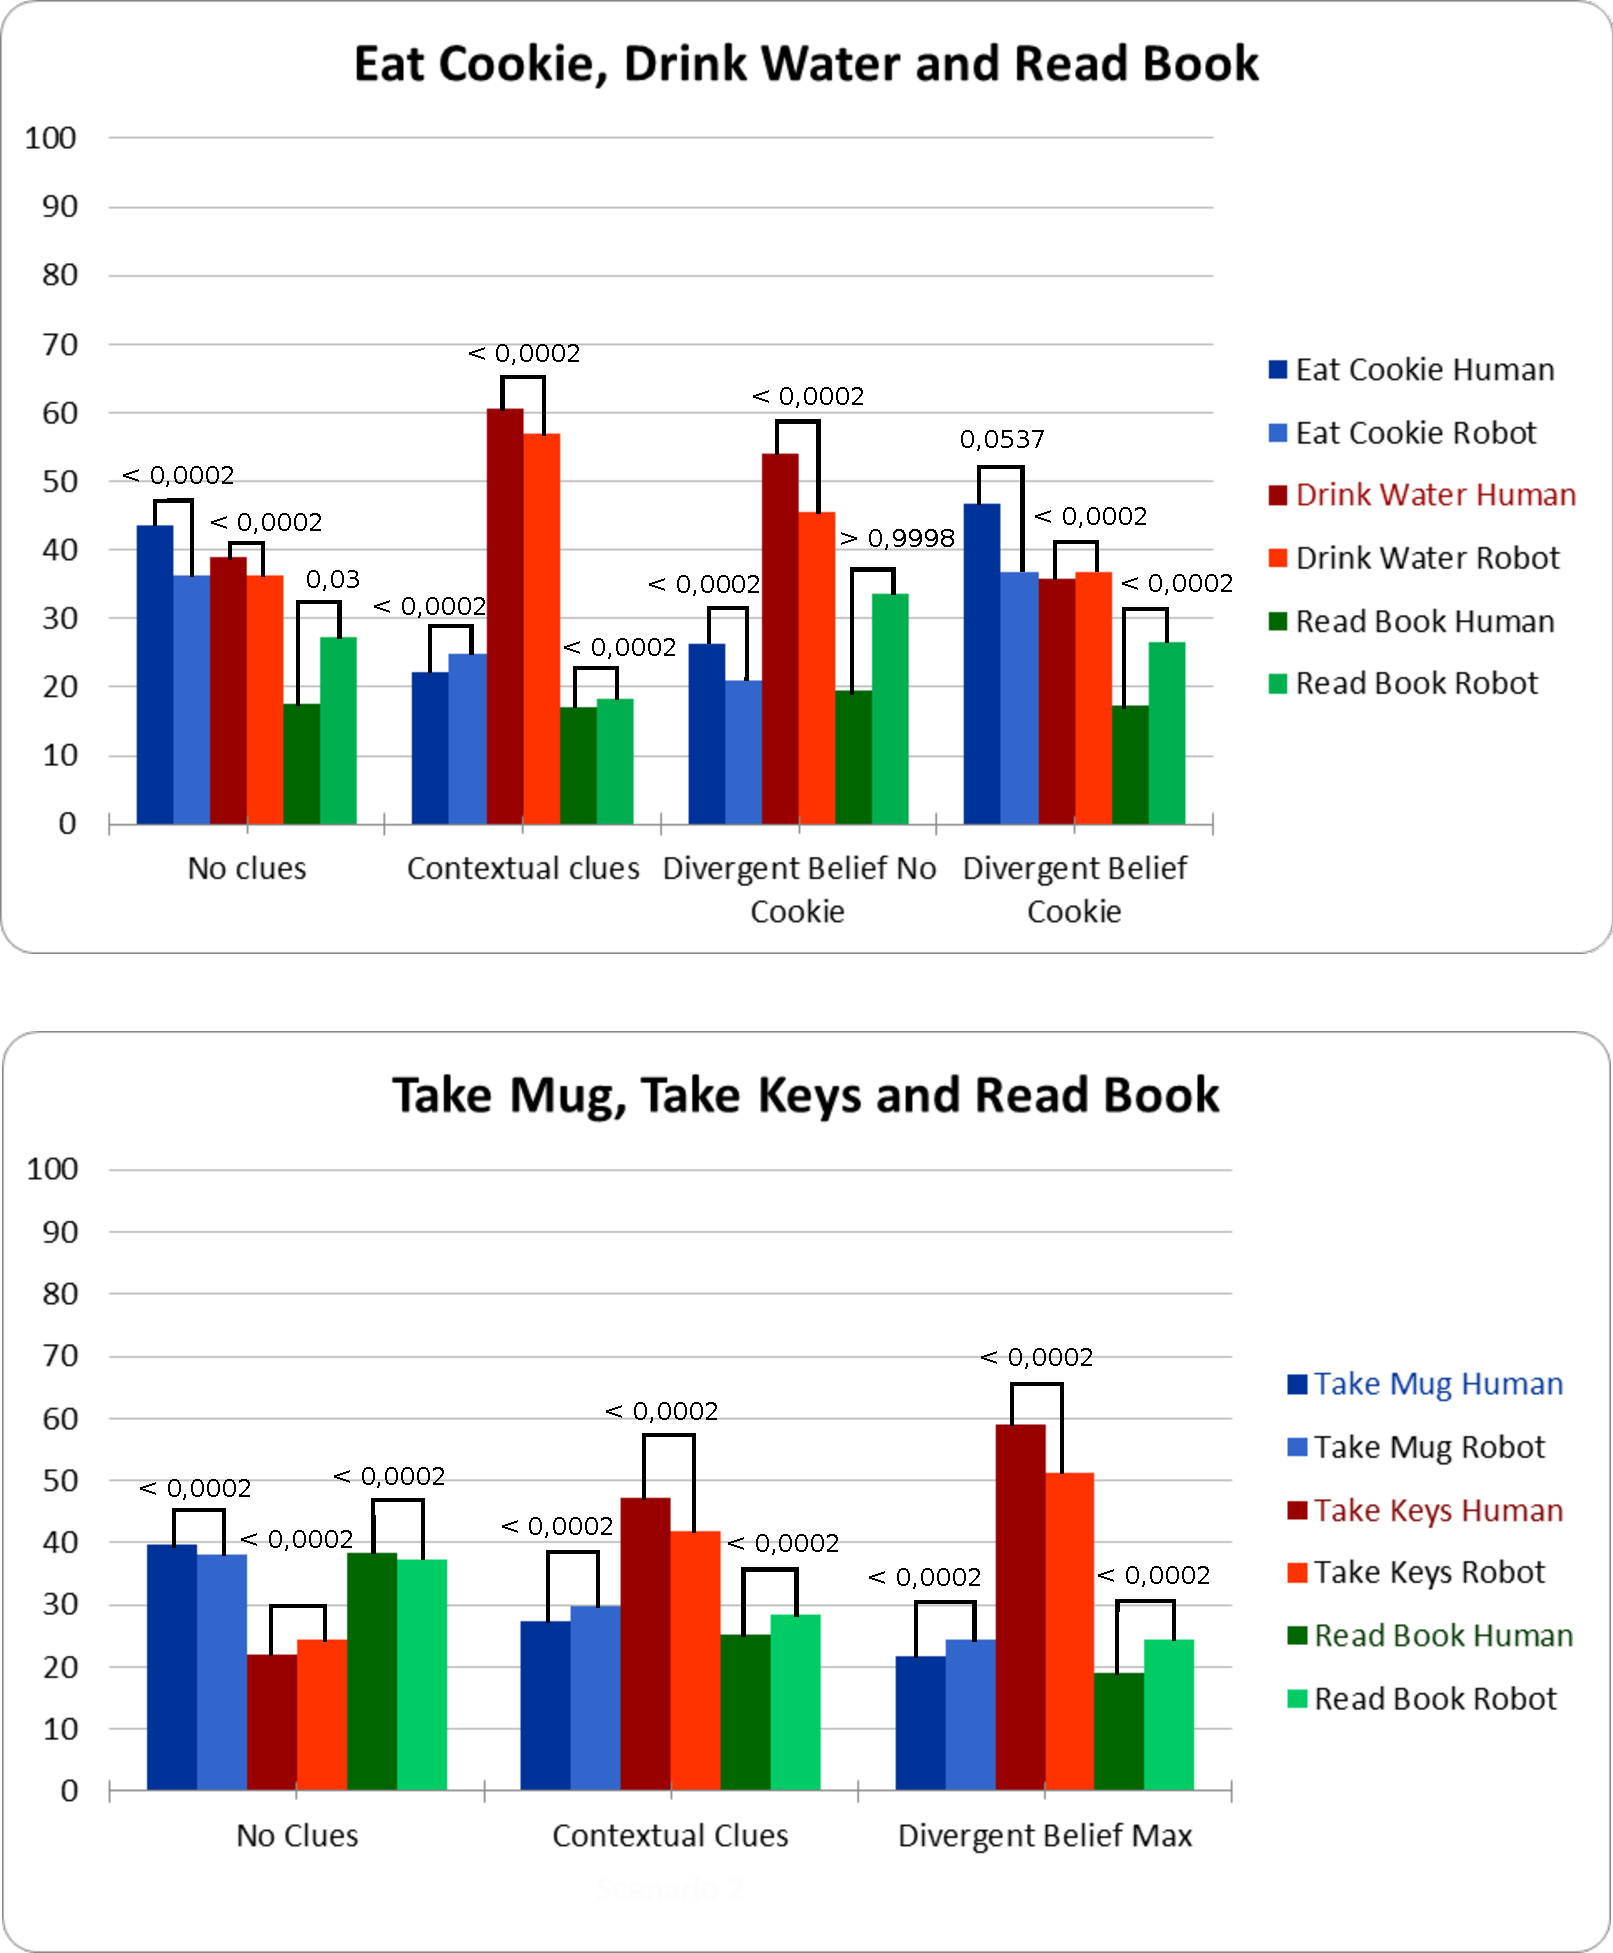
\includegraphics[clip,scale=0.32]{img/situation_assessment/pvalues1.pdf}
	\caption{Experiment results. Results from the two scenarios are represented as graphs. Intentions, as estimated by the humans and the robot, are represented by different colors, as shown in the legend of the graphs, with estimations of the same intention by the robot or the human placed in adjacent position. Each column represents the likelihood of an intention, expressed as a percentile score. P-values from the equivalence tests are shown, linking the estimation of an intention by the humans and by the robot.}
	\label{fig:situation_assessment-user_study_results}
\end{figure}



 
\chapter{Inferring Human Intention and Reacting} % Main chapter title

\label{chapter:intention} % Change X to a consecutive number; for referencing this chapter elsewhere, use \ref{ChapterX}

\lhead{Chapter 3. \emph{Intention Recognition}} % Change X to a consecutive number; this is for the header on each page - perhaps a shortened title


\section{Introduction}
Another crucial skill to interact with humans is recognizing others' actions and goals. This process is is directly linked to modeling humans' beliefs, since, as explained by \cite{byom2013theory} ``as humans, we generally believe that others act in ways that are consistent with their beliefs and goals". 

The recognition of human activities is an important topic in computer science research, which can be studied at different levels. Anticipating human actions and movements allows the robot to adapt its behavior and proactively help humans, as studied in \cite{koppula2013anticipating}. 

Sequences of actions can be linked to plans, a well-known topic called plan recognition. Several approaches have been studied in this domain using, for example, classical planning \cite{ramirez2009plan}, probabilistic \cite{bui2003general} or logic techniques \cite{singla2011abductive}.

Other approaches that can be used to estimate the intention of a human are Interactive Partially Observed Markov Decision Processes (I-POMDP) and Inverse Learning. I-POMDP  \cite{gmytrasiewicz2004interactive} offer a rich framework that extends Partially Observed Markov Decision Processes (POMDP) in a multi-agent setting. Inference in these models can be extremely complex, but there have been attempts at solving this issue, like in \cite{doshi2009monte,hoang2013interactive}. 

Inverse Reinforcement Learning \cite{ng2000algorithms} formulates the problem of computing an unknown reward function of an agent after observing his behavior. This strategy has been applied, with Bayesian Networks (BN), in \cite{Nagai2015}, in order to learn the mental model of another agent, and choose appropriate actions for a relationship building task. A linked approach is inverted planning, which has been applied in a bayesian framework in \cite{baker2009action}  for human action understanding.

The use of contextual information can be used to further disambiguate complex situations. \cite{Liu2014} shows a system using BNs to understand users' intentions with an emphasis on contextual information. This BN is constructed using object affordances nodes (e.g. a cup can be washed or used for drinking), context nodes (e.g. it's a hot day, the cup was recently used), and intention nodes (e.g. drinking from a cup or washing it). The causal links between contexts and intentions are learnt through a user study, which uses an online questionnaire where participants need to rate the strenght of the connection betwen an intention and a context. The work does not study how to adapt this BN to complex plans, composed by sequences of actions.

It is very important to consider humans' beliefs when estimating their intentions. In a dynamic environment, agents can execute actions, modifying the state of the world without other agents being able to perceive the changes. Let us imagine a scenario. Bob comes back home from work and would like to relax while reading. He lays down on a sofa with a book, and reaches to a nearby table to grab his glasses. He does not know that his wife, during the day, moved the glasses to another room. If we would ignore Bob's beliefs on the world (i.e. he does not know that the glasses are not on the table) we could infer that, for example, Bob would like a drink while he is sitting on the sofa, or the tv remote controller. If, instead, we would know that Bob thinks his glasses are on the table (and we would use other contextual information perhaps, like Bob's habitudes) we would be able to correctly infer Bob's current intention, that is, taking his glasses, and warn him that they are not there, perhaps even fetching them for him. 

In robotics, an interesting framework that considers this issue is the Bayesian Theory of Mind \cite{baker2014modeling}, used to represent the inference process of an observer looking at another agent's behaviors. The acting agent is modeled as a POMDP, whose richness is able to represent its possible beliefs about the world. The observer's process is modeled as a DBN, built starting from the agent's POMDP but considering his reward function (that represents his desires) as hidden. The system has been tested against some alternative models and compared, in user studies, with human capacities, to understand how well it models theory of mind. Since the models used are quite complex, scalability in the model could be an issue. Also, the study is focused on a single-agent scenario, and does not consider collaborative problems.

Let us examine the two simulation-based systems that we already presented in the previous section, HAMMER ~\cite{demiris2007prediction}, and the architecture of \cite{BreazealGB09}, and see how these cognitive architectures are able to infer actions and intentions.

The HAMMER system is organized with couples of inverse and forward models.  Inverse models receive as input the goal and state of the system, producing the motor commands which are needed to achieve the goal. Forward models, instead, receive as input motor commands and compute the predicted future state. When these two models are linked, the forward model receives as input the motor commands produced by an inverse model. This link can form a loop, with the output of a forward model returning to its inverse model, which can adjust a range of parameters if the predicted future state does not match exactly the desired state. These models can be organized in parallel schemas and used to recognize actions performed by a demonstrator. 

In this case, the demonstrator's current state, as perceived by the robot, is fed in the inverse models, which in turn sends their output to their forward models. The state predicted by the forward models are compared with the demonstrator's state at the next time step. This comparison produces a score, which can be used to infer the most likely action performed. 

Forward and inverse models can be organized in hierarchical schemas, to infer actions and plans. The complexity of these schemas could be quite significant, particularly when trying to recognize a goal which can be achieved in many different ways, depending on the context. 

\cite{BreazealGB09} uses a similar ideas, where the all the possible robot movements are represented as a graph of connected poses, with arcs representing possible transitions between the poses. This graph is used both to represent the robot's movements and to map observed trajectories. Tasks are represented as schemas, which can be organized in sequential and hierarchical structures to represent complex goals.

 When trying to infer an agent's intention the robot looks for a schema whose motor action matches the observed activities of the agent. After that, the schema is traversed in reverse in order to try to determine the real intention. The system is not able to deal with ambiguities, and this algorithm stops if it comes to a point where there is more than a possible explanation for the current behavior. 

An example of non simulation-based system in this topic can be seen in \cite{talamadupula2014coordination}. This architecture is used to coordinate human-robot teams, based on intention recognition and belief modeling. Creating and maintaining beliefs is handled using the strategy explained in ~\cite{scheutz2013computational}, presented in the previous subsection. Prediction of other humans intentions' is based on the plan recognition algorithm of \cite{ramirez2009plan}. While this algorithm uses efficient replanning to increase its efficiency, in complex domains, where the users have many different strategies to achieve a goal, the system would need to execute frequent replans to infer the actual strategy chosen by the user, which can be expensive.


\section{Intention and Action Inference}
\label{sec:situation_assessment-intention_recognition}
Understanding what others are doing is an important skill for a robot partner. We have designed a module that is able, through inference, to recognize human actions and connect them to possible intentions. Actions and intentions are evaluated with perspective taking using the humans' belief models, and further disambiguated by taking into account the current context.

In order to perform this reasoning, we will provide the following information to the robot: a list of known contexts, a list of known intentions, a list of known actions, a set of observations of human actions, and a belief model of humans and of the robot itself.

We introduce a simplification in our model: at each time step, a human can execute only one action and has only one intention, decreasing the ambiguities in the inference process.

We propose, as central model used for intention estimation, a framework based on BNs. We call our implementation of BN an Intention Graph (IG).
An IG is linked to a specific human, and composed by the following layers of nodes:
\begin{itemize}
\item Context Nodes: these nodes represent contextual information, modeled as boolean variables (e.g. HotDay, ColdDay).
\item Intention Nodes: these boolean nodes represent the set of possible intentions. Each intention can conditionally depend on several contexts.
\item Action Nodes. This is the set of human actions whose preconditions are satisfied when the IG is created. Each of these nodes is conditionally dependent on all the intention nodes. 
\item Observation Nodes. We associate to each action a different set of observation nodes, that depend conditionally on the associated action node. For example, the distance of a human from the \textit{target} of an action can be an Observation Node.
\end{itemize}

In a typical usage, the robot will create, for each monitored human, an IG, formed by the Context and Intention Nodes, which we consider statically known by the robot, and a variable list of Action and Observation nodes, which depends on the human's belief model. The robot will create action nodes for each known action whose $preconditions$ are satisfied in the human's belief model, and their related Observation Nodes. These IGs will be updated every time that an agent performs an action, creating and removing Action and Observation nodes, depending on the state of the world after the action was performed.

When monitoring a human, we set Context Nodes and Observation Nodes as \textit{evidence}, considering them observable by the robot. These information will allow us to have a good estimation of the most likely actions and intentions of the human, as explained in subsection \ref{sec:situation_assessment-intention and action inference}. 


An example of IG, taken from an experiment, can be seen in figure \ref{fig:situation_assessment-intention_graph}. In the following paragraphs, we will explain the role of these layers of nodes, and how the conditional dependencies between them are computed. After that, we will show an example showing how an IG is created and updated following a sequence of human actions, and how the robot is able to use it to infer the most likely human intention.

 \begin{figure}[ht!]
	\centering
	\includegraphics[trim={2cm 11cm 11cm 17cm},clip,scale=0.45]{img/situation_assessment/cookieScenario.pdf}
	\caption[Intention Graph]{A scene from our experiment. The yellow arrows show possible actions and their associated probabilities. The diagram represents the current IG. Green circles represent evidence nodes and blue circles other nodes. For the Context Nodes (top of the graph), we represented nodes with a false value as greyed out, and nodes with a true value as green. The most likely nodes in the graph are represented with a glowing effect. The observation nodes were compressed in a single block to simplify the diagram}
	\label{fig:situation_assessment-intention_graph}
\end{figure}

\subsection{From Contexts to Intentions}
We introduce a set of contexts in our domain. We consider as context any information that can be used to characterize and motivate an intention \cite{abowd1999towards}. We model a context  as a fact, which can assume different values and influences the probability of a user having a particular intention. For example, we imagine that a human is more likely to be cooking at dinner time, or to drink a hot mug of tea on a cold day.

Contextual nodes can directly influence one or more Intention nodes. In this work, we chose to learn these conditional dependencies from humans, as explained in section \ref{sec:situation_assessment-experiments}.

\subsection{From Intentions to Actions}
\label{sec:situation_assessment-action_evaluation}
To understand how actions are linked to intentions the robot needs to answer the following question: what actions would a human take, in this situation, given his belief of the world, in order to achieve its intention?
Our idea is based on the principle of rationality \cite{Dennet1989}, which states that agents tend to choose the most efficient actions, taking into account their beliefs about the world, in order to achieve their desires.

In \cite{Blakemore2001}, the authors explain that ``the attribution of intentions to actions might rely on simulating the observed action and mapping it into representations of our own intention". We represent this idea by providing the robot with a set of planning models. Each one of these planning models is related to an intention, and represents all the known plans to achieve its linked goal. In this way, we can estimate how much the current human actions are compatible with the plans related to an intention.

In our implementation, for each intention known by the robot, we will create an associated Markov Decision Process (MDP), to represent all the possible plans linked to this intention. After solving the set of MDPs we will use the calculated action value function \(Q(s,a)\), to create conditional dependencies between Intention and Action nodes in the IG. We define \(P(a|I_i=1)\), the probability that action $a$ will be performed if intention $I_i$ is true, as as:
\begin{equation}
 P(a|I_i=1)=\frac{Q_i(s,a)}{\sum_b(Q_i(s,b))}
\end{equation}
  where we normalize the value function $Q_i(s,a)$ for intention $i$ and action $a$ in the human's belief state $s$, over the value function $Q_i(s,b)$ calculated on all the monitored actions $b$. 

%   We can extend this calculation to the case where a generic number of intentions are true to compute the probabilities of action nodes: 
% \begin{equation}
%   P(a|I_1,I_2,...,I_m)=\frac{\sum_{i:I_i=1}Q_i(s,a)}{\sum_b\sum_{i:I_i=1}Q_i(s,b)}
% \end{equation}

The key idea in this problem is to use the human's belief state as input for the MDPs' value functions. In this way we are using perspective taking at a planning level, since the human action will be consistent with his intention in his own belief state but may be not optimal, irrelevant, or even dangerous in the real world (e.g. in case of wrong belief).

Our idea is similar to \cite{karami2010human}. In this work, the robot planning model is a POMDP, where the human intention is a hidden variable. The transition function for the human intention is computed starting from the action values obtained from a set of human MDPs, that simulate human policies related to different intentions. In this work, we used a BN for the inference process, instead of a POMDP. This allows us to include in a simple way more information in the inference process, such as context, and to separate the mechanisms used for inference and for the robot's actions. Also, we improve the recognition process by including the belief state of the human.

\subsection{From Actions to Observations}
Intentions will be inferred from human actions, so the robot needs to monitor their execution. For each Action Node we can define a different set of Observation Nodes, which depend on the specific actions. Typical examples are: the distance of the human's body from the action's $target$, its variation, the distance of the human's hand from the action's $target$, and its variation. The conditional dependencies of the Observation Nodes are precomputed.

\subsection{Intention and Action Inference}
\label{sec:situation_assessment-intention and action inference}
We assume, in this work, that at each moment a human can only execute a single action, and the robot will react only to his most likely intention. The most likely action and intention are inferred from the BN in the following way. We call $P(n)$ the inferred probability of a node $n$, $B(n)$ the set of brothers of $n$ (that is, nodes on the same layer), and $\delta_1$, $\delta_2$ two thresholds. The robot selects the most likely action and intention following these rules: 
\begin{itemize}
\item  \(P(n_i)>\delta_1\) 
\item  \(\forall b \in B(n_i): P(n_i)>P(b)+\delta_2\), where $n_i$ is the node associated to the interested intention or action.
\end{itemize}


To infer that an action has been performed, the robot uses an estimation of the action's probability and geometrical reasoning. For example, the robot infers that a human has taken a bottle if his hand is closer to it than a threshold $\sigma$  and the action's probability in the IG respect the previous rules. For another example, the robot infers that a human has mixed some ingredients in a bowl if his hand approaches the bowl and then leaves after some seconds, always taking into account the probability of the action in the IG.

When the robot infers that an action has been performed, it updates the world state with its $postconditions$, triggering an update on the beliefs of all present agents. The current human intention is recorded in the Database, and will be used by the Goal Management layer.

 \begin{figure}[ht!]
	\centering
	\includegraphics[scale=0.8, trim={0 4cm 0 0}]{img/situation_assessment/pick.pdf}
	\caption[Actions and world update]{The human picks an object and the robot updates accordingly the world state. The spheres surrounding objects show when the human's hand is considered to be near an object.}
	\label{fig:situation_assessment-pick}
\end{figure}


\subsection{Proactive Behaviors}
\label{subsec:situation_assessment-proactive_behaviors}
Information about the most likely intention and action will be introduced in the database, to be read by the Goal Management Layer. Based on this information, the robot can execute two different proactive behaviors: correcting the belief state of the human, and proactively helping him to achieve his task.

\subsubsection{Correcting Belief State}
Having a wrong or incomplete belief on the world state can lead agents to execute non optimal, useless, or even dangerous actions. The robot needs to detect these situations in order to warn the human. For example Greg could search for his glasses in a wrong location if he does not know that they were moved, or could touch a hot object if he does not know its temperature.

 The robot assumes that it always holds a correct belief state. Our solution uses the expected action rewards introduced in \ref{sec:situation_assessment-action_evaluation}. The idea is comparing the expected reward for performing an action according to the human and the robot's belief states. To formalize: we compare the action values \(Q_m(s_h,a_h)\) and \(Q_m(s_r,a_h)\), where $m$ is the most likely intention,  $s_h$ and $s_r$ are the robot's and human's belief state, and $a_h$ is the most likely action. If these values are not equal the human expects a different outcome from its action than what should actually happen. 

We propose a simple solution, where the robot warns the human of the detected divergent belief for that action. For example, Bob wants to drink tea from a closed, opaque bottle, which the robot knows is empty (perhaps because another agent drank the last glass), while Bob does not. When he approaches the bottle, the robot detects that his most likely intention is to drink tea. The system calculates the expected rewards from taking the bottle in the two belief models and obtains different values. The system checks the facts related to the attributes associated to the bottle in the two mental models, and extracts the differences. Using this information, the robot corrects the divergent belief, informing the human that the bottle is now empty. 

In our system, the Goal Management layer will detect these situations, by reading the Database, and choose a \textit{warn agent} goal (as will be explained in chapter \ref{chapter:goal_management}).

In a real scenarios, the human might have several divergent beliefs at the same time. While the robot could inform the human as soon as it detects a divergent belief, it would risk overloading the human with unneeded information. For example, Greg might not know that his wife drank a mug of coffee or moved the remote control to the table, but maybe he will not need these information in the near future. We chose, with this approach, to give information about a divergent belief only when it risks impacting the action of a human.

\subsubsection{Performing a part of the plan}
There are situations in which the robot should help the human achieve its goal by physically acting. The Goal Management layer will consider new inferred intentions as possible goals for the robot, and will communicate with the Plan Production and Management layer to achieve them, as explained in chapters \ref{chapter:goal_management}, \ref{chapter:plan_management}, and \ref{chapter:plan_execution}. 


\subsection{Intention Graph Example}

\subsubsection{Scenario}
We will now show an example of use of an IG. We start by defining a scenario with a human, Greg, and two possible intentions: drinking water and reordering a table, by moving all the objects on top of it to the kitchen. We set three different locations: a \textit{table}, a \textit{shelf}, and a \textit{kitchen}. We consider two objects: a \textit{glass} and a \textit{bottle}. The \textit{bottle} and the \textit{glass} can contain water, but the \textit{bottle} is opaque and Greg can not observe if there is water or not in it. Of course, this scenario is not realistic and is chosen just to illustrate the IG. In a real situation Greg would notice that the bottle is empty when taking it, because it would be too light, or when opening it.
At the start of the scenario, Greg is at the \textit{shelf}, the \textit{bottle} and \textit{glass} are on the \textit{table}, and the they are both empty. 

We set a situation of divergent belief, where Greg does not know that the bottle is empty, but the robot has this information. 
We introduce two predicates: \textit{isAt}, that represented the location of an object, and can assume the values \textit{TABLE}, \textit{SHELF}, and \textit{KITCHEN}; and \textit{capacity}, which represents if the object contains water, and can assume the values \textit{0}, and \textit{1}. 
The belief models of Greg and of the robot are shown in table ~\ref{table:situation_assessment-ig_bm}, while the set up for this scenario is shown in figure \ref{fig:situation_assessment-ig_scenario}.

 \begin{table}[h!]
\centering
\scriptsize
\renewcommand{\arraystretch}{1.3}
\begin{tabular}{|c|c|}
\hline
Robot & Human \\ \hline \hline
GLASS isAt TABLE  & GLASS isAt TABLE \\ \hline
BOTTLE isAt TABLE & BOTTLE isAt TABLE \\ \hline
GLASS capacity 0  & GLASS capacity 0  \\ \hline
BOTTLE capacity 0 & BOTTLE capacity 1 \\ 
\hline
\end{tabular}
\caption[Belief models in the IG scenario]{Belief models for Greg and for the robot in the Intention Graph example scenario. There is a divergent belief situation, where Greg does not know that the bottle is currently empty, represented by the fact \textit{BOTTLE capacity VALUE} }
 \label{table:situation_assessment-ig_bm}    
\end{table}



 \begin{figure}[ht!]
	% \centering
	\includegraphics[scale=0.5]{img/situation_assessment/ig_scenario.pdf}
	\caption[IG Example Scenario]{The image shows the set-up for this example scenario. The locations are represented as different rectangles. Greg is represented as a black circle. The glass and bottle are represented, respectively, by a blue circle and a red circle.}
	\label{fig:situation_assessment-ig_scenario}
\end{figure}

We introduce two contexts in the scenario: \textit{HotDay}, representing the fact that the day is particularly warm, and \textit{AlreadyDrank}, representing the fact that the human has recently drank water.

We introduce this possible set of actions in the scenario: taking the bottle, taking the glass, filling the glass using the bottle, drinking from the glass, moving to the kitchen, moving to the table, placing the objects in different locations. We simplify this set to only include the actions relevant to this example, and so we do not include the possibilities for Greg to refill the bottle with water. Also, we consider that Greg can only take a single object at the moment. 

\subsubsection{Building the Intention Graph}

We build a starting IG with the following nodes:
\begin{itemize}
	\item Context Nodes: \textit{HotDay}, \textit{AlreadyDrank}.
	\item Intention Nodes: \textit{DrinkWater}, \textit{ReorderTable}.
	\item Action Nodes: \textit{MoveTable}, \textit{MoveKitchen}. These two actions are introduced in the IG because they are the only ones whose $preconditions$ are currently satisfied, since Greg can move in any location where he is not at the moment.
	\item Observation Nodes: \textit{BodyDistanceTable}, \textit{TowardTable}, \textit{BodyDistanceKitchen}, \textit{TowardKitchen}. The \textit{BodyDistance} nodes represent the distance between Greg and an object, and can assume the values \textit{close}, \textit{medium}, \textit{far}, \textit{out of range}. The \textit{Toward} nodes are \textit{true} if the distance between \textit{Greg} and the object is decreasing, and false otherwise.
\end{itemize}


In this scenario, we precompute the probability table of the causal links between Context Nodes and Intention Nodes, and between Action Nodes and Observaton Nodes. We set a causal link between \textit{HotDay} and \textit{DrinkWater}, and one between \textit{AlreadyDrank} and \textit{ReorderTable}. In both cases, we use the following probability table:

 \begin{table}[h!]
\centering
\begin{tabular}{|c|c|c|}
\hline
Context & \multicolumn{2}{|c|}{Intention} \\ \hline \hline
& 0 & 1 \\ \hline
0  & 0.6 & 0.4 \\ \hline
1 & 0.4 & 0.6 \\ \hline
\end{tabular}
\caption[Belief models in the IG scenario]{Conditioned probabilities of the Intention Nodes in the IG example scenario.}
 \label{table:situation_assessment-ig_intention}    
\end{table}

We consider as slightly more likely that Greg wants to drink water in a Hot Day, and that he wants to reorder the table if he drank recently.

We set a causal link between each action and its observation nodes. For example, \textit{MoveTable} will have a causal link with \textit{BodyDistanceTable} and \textit{TowardTable}. In both actions, we use the following probability tables:

 \begin{table}[h!]
\centering
\begin{tabular}{|c|c|c|}
\hline
Action & \multicolumn{2}{|c|}{Toward} \\ \hline \hline
& 0 & 1 \\ \hline
0  & 0.8 & 0.2 \\ \hline
1 & 0.2 & 0.8 \\  \hline
\end{tabular}
\caption[Belief models in the IG scenario]{Conditioned probabilities of the Toward Nodes in the IG example scenario.}
 \label{table:situation_assessment-ig_toward}    
\end{table}

 \begin{table}[h!]
\centering
\begin{tabular}{|c|c|c|c|c|}
\hline
Action & \multicolumn{4}{|c|}{Distance} \\ \hline \hline
& Close & Medium & Far & Out of Range \\ \hline
0  & 0.16 & 0.2 & 0.25 & 0.39 \\ \hline
1 & 0.39 & 0.25 & 0.2 & 0.16 \\ \hline
\end{tabular}
\caption[Belief models in the IG scenario]{Conditioned probabilities of the Distance Nodes in the IG example scenario.}
 \label{table:situation_assessment-ig_distance}    
\end{table}

If Greg is executing an action, it  more likely that he is moving toward the action's $target$. For example, the \textit{MoveTable} action is more likely the closer Greg is to the table and if the distance to it is decreasing.

\subsubsection{Building the Human MDPs}

To set the conditioned probabilities between Intention and Action Nodes, we created two different MDPs, each related to one of the intentions. We will now show the state space $S$, action set $A$ and reward function $R$  of the two MDPs. We do not include the transition function of the model as it is extensive and does not help understanding this example.

\begin{itemize}
\item DrinkWater:
\begin{itemize}
\item $S$: $\{agent\_isAt, glass\_isAt, bottle\_isAt, bottle\_capacity, glass\_capacity\}$.
\item $A$: $\{agent\_move\_table, agent\_move\_kitchen, agent\_move\_shelf, agent\_take\_bottle, \\ 
agent\_take\_glass, 
agent\_fill\_glass\_bottle, agent\_drink\_glass, agent\_place\_bottle\_table, \\ agent\_place\_bottle\_kitchen, agent\_place\_bottle\_shelf, agent\_place\_glass\_table, \\ agent\_place\_glass\_kitchen, agent\_place\_glass\_shelf\}$.
\item $R(s,a)=1000 \quad \text{if} \\
glass\_isAt==agent\_isAt \; \text{AND} \; glass\_capacity==1  \; \text{AND} \; a==agent\_drink\_glass$.
\end{itemize}


\item ReorderTable:
\begin{itemize}
\item $S$: $\{agent\_isAt, glass\_isAt, bottle\_isAt\}$.
\item $A$: $\{agent\_move\_table, agent\_move\_kitchen, agent\_move\_shelf, agent\_take\_bottle,\\ agent\_take\_glass, 
agent\_place\_glass\_kitchen, agent\_place\_bottle\_kitchen\}$.
\item $R(s,a)=1000 \quad \text{if} \\
(glass\_isAt==kitchen \; \text{AND} \; bottle\_isAt==human \; \text{AND} \; a==human\_place\_bottle\_kitchen)  \\
 \text{OR} \\
 (glass\_isAt==human \; \text{AND} \; bottle\_isAt==kitchen \; \text{AND} \; a==human\_place\_glass\_kitchen)$.
\end{itemize}
\end{itemize}

After solving these MDPs we used their action value functions to compute the conditioned probabilities for the Action Nodes, as shown in \ref{sec:situation_assessment-action_evaluation}.

\subsubsection{Simulated Run}

We will now show a simulated run of this scenario in three steps. This run was created by introducing a stream of observations in the system, including the actions that Greg will perform. We consider that Greg's intention in this example is \textit{Drink Water}. We will conduct three different tests for each step:
\begin{itemize}
	\item Test 1. We create the IG using the human's mental belief state to compute the causal links between action and intention nodes. We do not use context to help disambiguate the intentions.
	\item Test 2. We add contextual information to Test 1, setting \textit{HotDay} to \textit{true} and \textit{RecentlyDrank} to \textit{false}.
	\item Test 3. We do not use contextual information and use the robot's mental belief state to compute the causal links between action and intention nodes. This means that the robot will evaluate Greg's action by considering that he knows that the bottle is currently empty (even though he does not know).
\end{itemize}

We will now describe and discuss these stages:
\begin{itemize}
	\item Greg is approaching the \textit{table}, as shown in figure ~\ref{fig:situation_assessment-ig_exp1}. The observations are updated correspondigly, and the probabilities of the actions are computed. The action \textit{MoveTable} has the highest probability. 
		\begin{itemize}
			\item Test 1. At this stage, the system is not able to infer the correct intention. Greg could be going to the \textit{table} to take the objects and bring them to the \textit{kitchen} or to drink water. The probability of the two intentions is both 0.50.
			\item Test 2. By using context, the system is already able to infer the correct intention. The probability of \textit{DrinkWater} becomes 0.69, and that of \textit{ReorderTable} 0.3. The robot could already fire a proactive behavior to inform Greg that the \textit{bottle} is, in fact, empty.
			\item Test 3. Without context, the system thinks that Greg is trying to reorder the table, since it is not possible to drink water because the \textit{bottle} is empty. The system would infer a wrong intention.
		\end{itemize}
	\item Greg has arrived to the \textit{table}, as shown in figure as shown in figure ~\ref{fig:situation_assessment-ig_exp2}. The $postconditions$ of the action are added to the mental models of the robot and of Greg, changing Greg's location. The system creates a new IG, setting as actions those whose $preconditions$ are now satisfied: \textit{MoveKitchen}, \textit{MoveShelf}, \textit{TakeGlass}, and \textit{TakeBottle}. At this point, Greg's hand moves toward the \textit{bottle}, and the observations nodes are set appropriately.
		\begin{itemize}
			\item Test 1. The system is still not able to disambiguate between the two intentions. Greg could be taking the  \textit{bottle} to fill the \textit{glass} or to bring it to the \textit{kitchen}.
			\item Test 2. In this case, the context is still providing the missing information to understand that Greg wants to drink water.
			\item Test 3. In this case, since it is not possible to drink water in the robot's mental belief, the system is still inferring the wrong intention.
		\end{itemize} 
	\item Greg has taken the \textit{bottle}, and is now moving it to the \textit{glass}, as shown in figure ~\ref{fig:situation_assessment-ig_exp3}. A new IG is created, containing the actions that are now executable: \textit{MoveKitchen}, \textit{MoveShelf}, \textit{PlaceBottleTable}, and \textit{FillGlass}. In test 3, the IG created would not contain the action to fill the glass with water, since it is not executable in the robot's mental belief model, where the \textit{bottle} is empty.
		\begin{itemize}
			\item Test 1. At this point, the system has enough information to understand that Greg's intention is \textit{DrinkWater}, which assumes a probability of 0.90. The system can now fire a proactive behavior, with the robot informing Greg of the divergent belief. Even tought the action \textit{PlaceBottleTable} and \textit{FillGlass} could be ambiguous from a geometric point of view (since in both cases, the arm of the human will approach the table), the system could infer that the action performed was \textit{FillGlass} since it is more \textit{useful} in the current situation and with the considered intentions.
			\item Test 2. Context confirms this intention, bringing the probability to 0.99.
			\item Test 3. In this case, Greg's movement would not be understood, since in the robot's mental belief model it is not possible to fill the glass with water.
		\end{itemize}
\end{itemize}

 \begin{figure}[ht!]
	\centering
	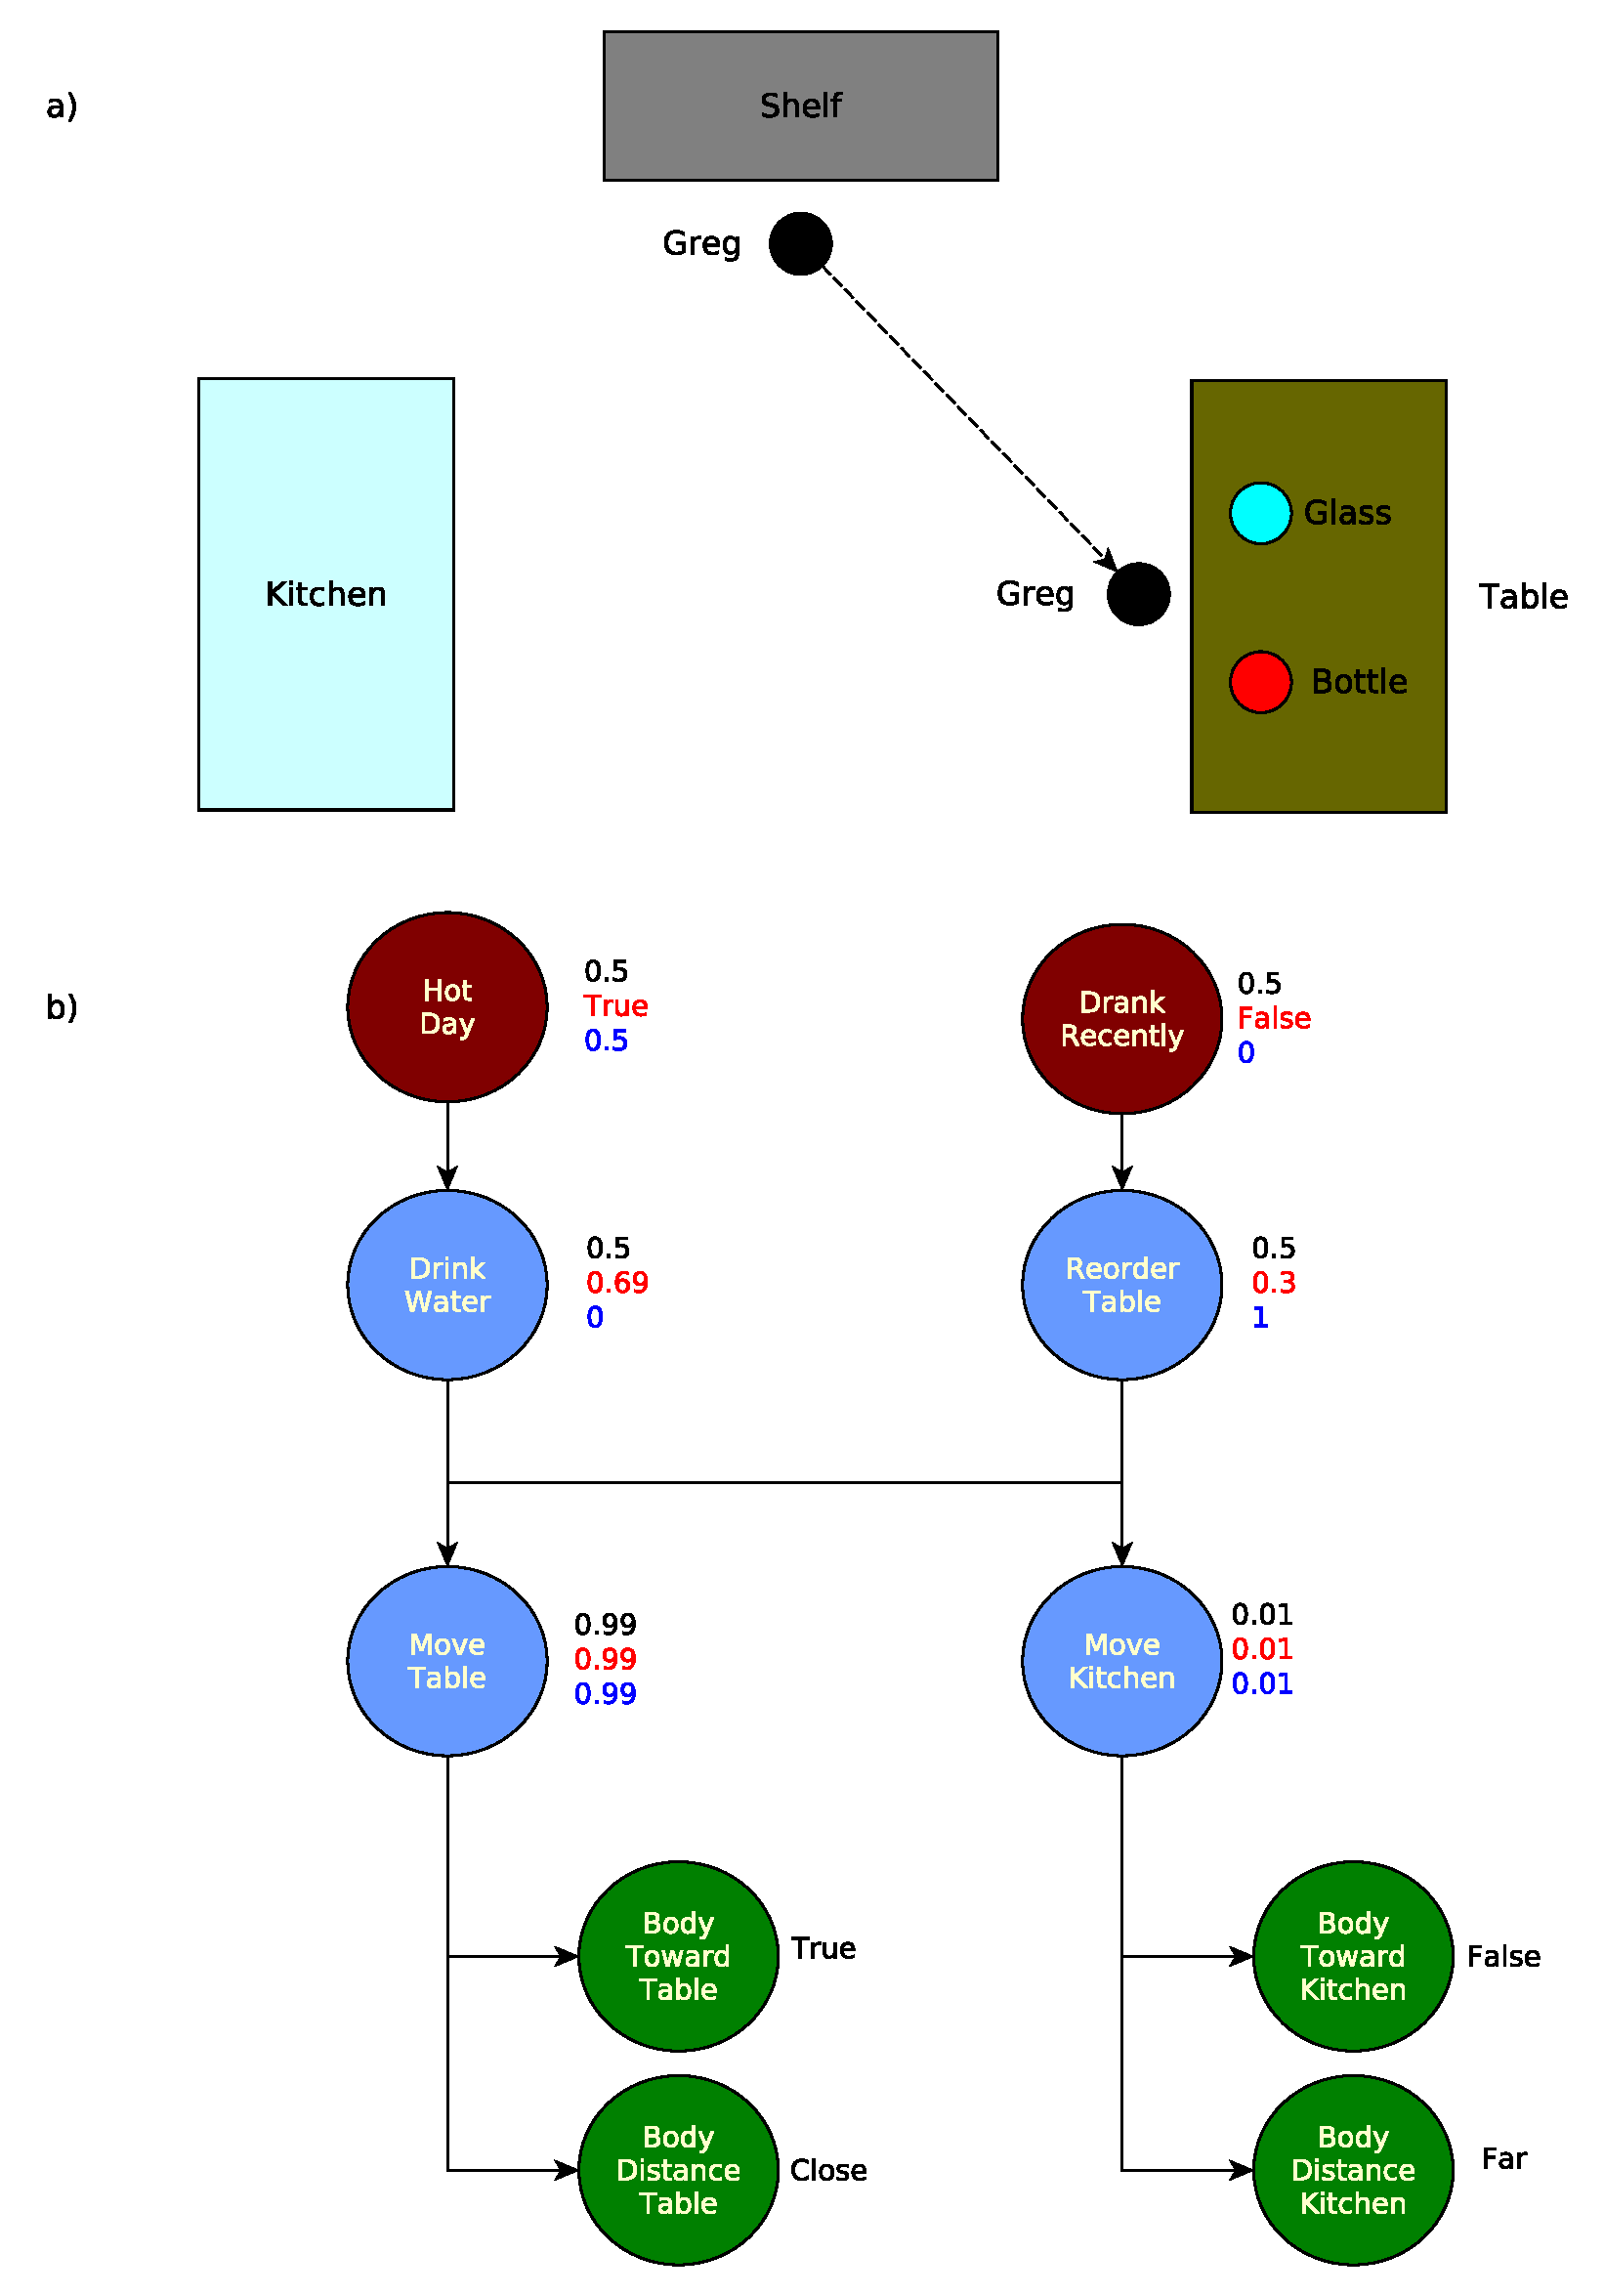
\includegraphics[scale=0.4]{img/situation_assessment/ig_exp1.pdf}
	\caption[IG Example 1]{a) Greg, represented as a black circle, is approaching the table. The two black circles correspond to his starting and ending location, with the dotted arrow showing the direction. b) The corresponding IG graph. Nodes are represented as circles and causal links as arrows. Intention and action nodes as represented as blue. Observation nodes are represented as green to show that we consider them as evidence, fixing their values. Context nodes are represented in yellow to mean that in the first and third test they are treated as standard nodes, and in the second as evidence.
 	 For each node we show the probability that its value is true or its current value, if it is treated as evidence. We show three different values for each node: the black one shows the value if we compute the probability by using the human's mental belief (test 1), the red if we use the human's mental belief and treat context nodes as evidence (test 2), and the blue if we do not use context and use the robot's mental belief for the computation (test 3). Test 1 shows that at this point the system is not able to disambiguate between the two intention, which have a value of 0.50. Test 2 shows that context would help the robot to infer correctly the intention. Test 3 shows that by not using the human's mental belief the robot would discard the drink water intention, considering it not achievable.}
	\label{fig:situation_assessment-ig_exp1}
\end{figure}

\clearpage

\hfill
 \begin{figure}[ht!]
	\centering
	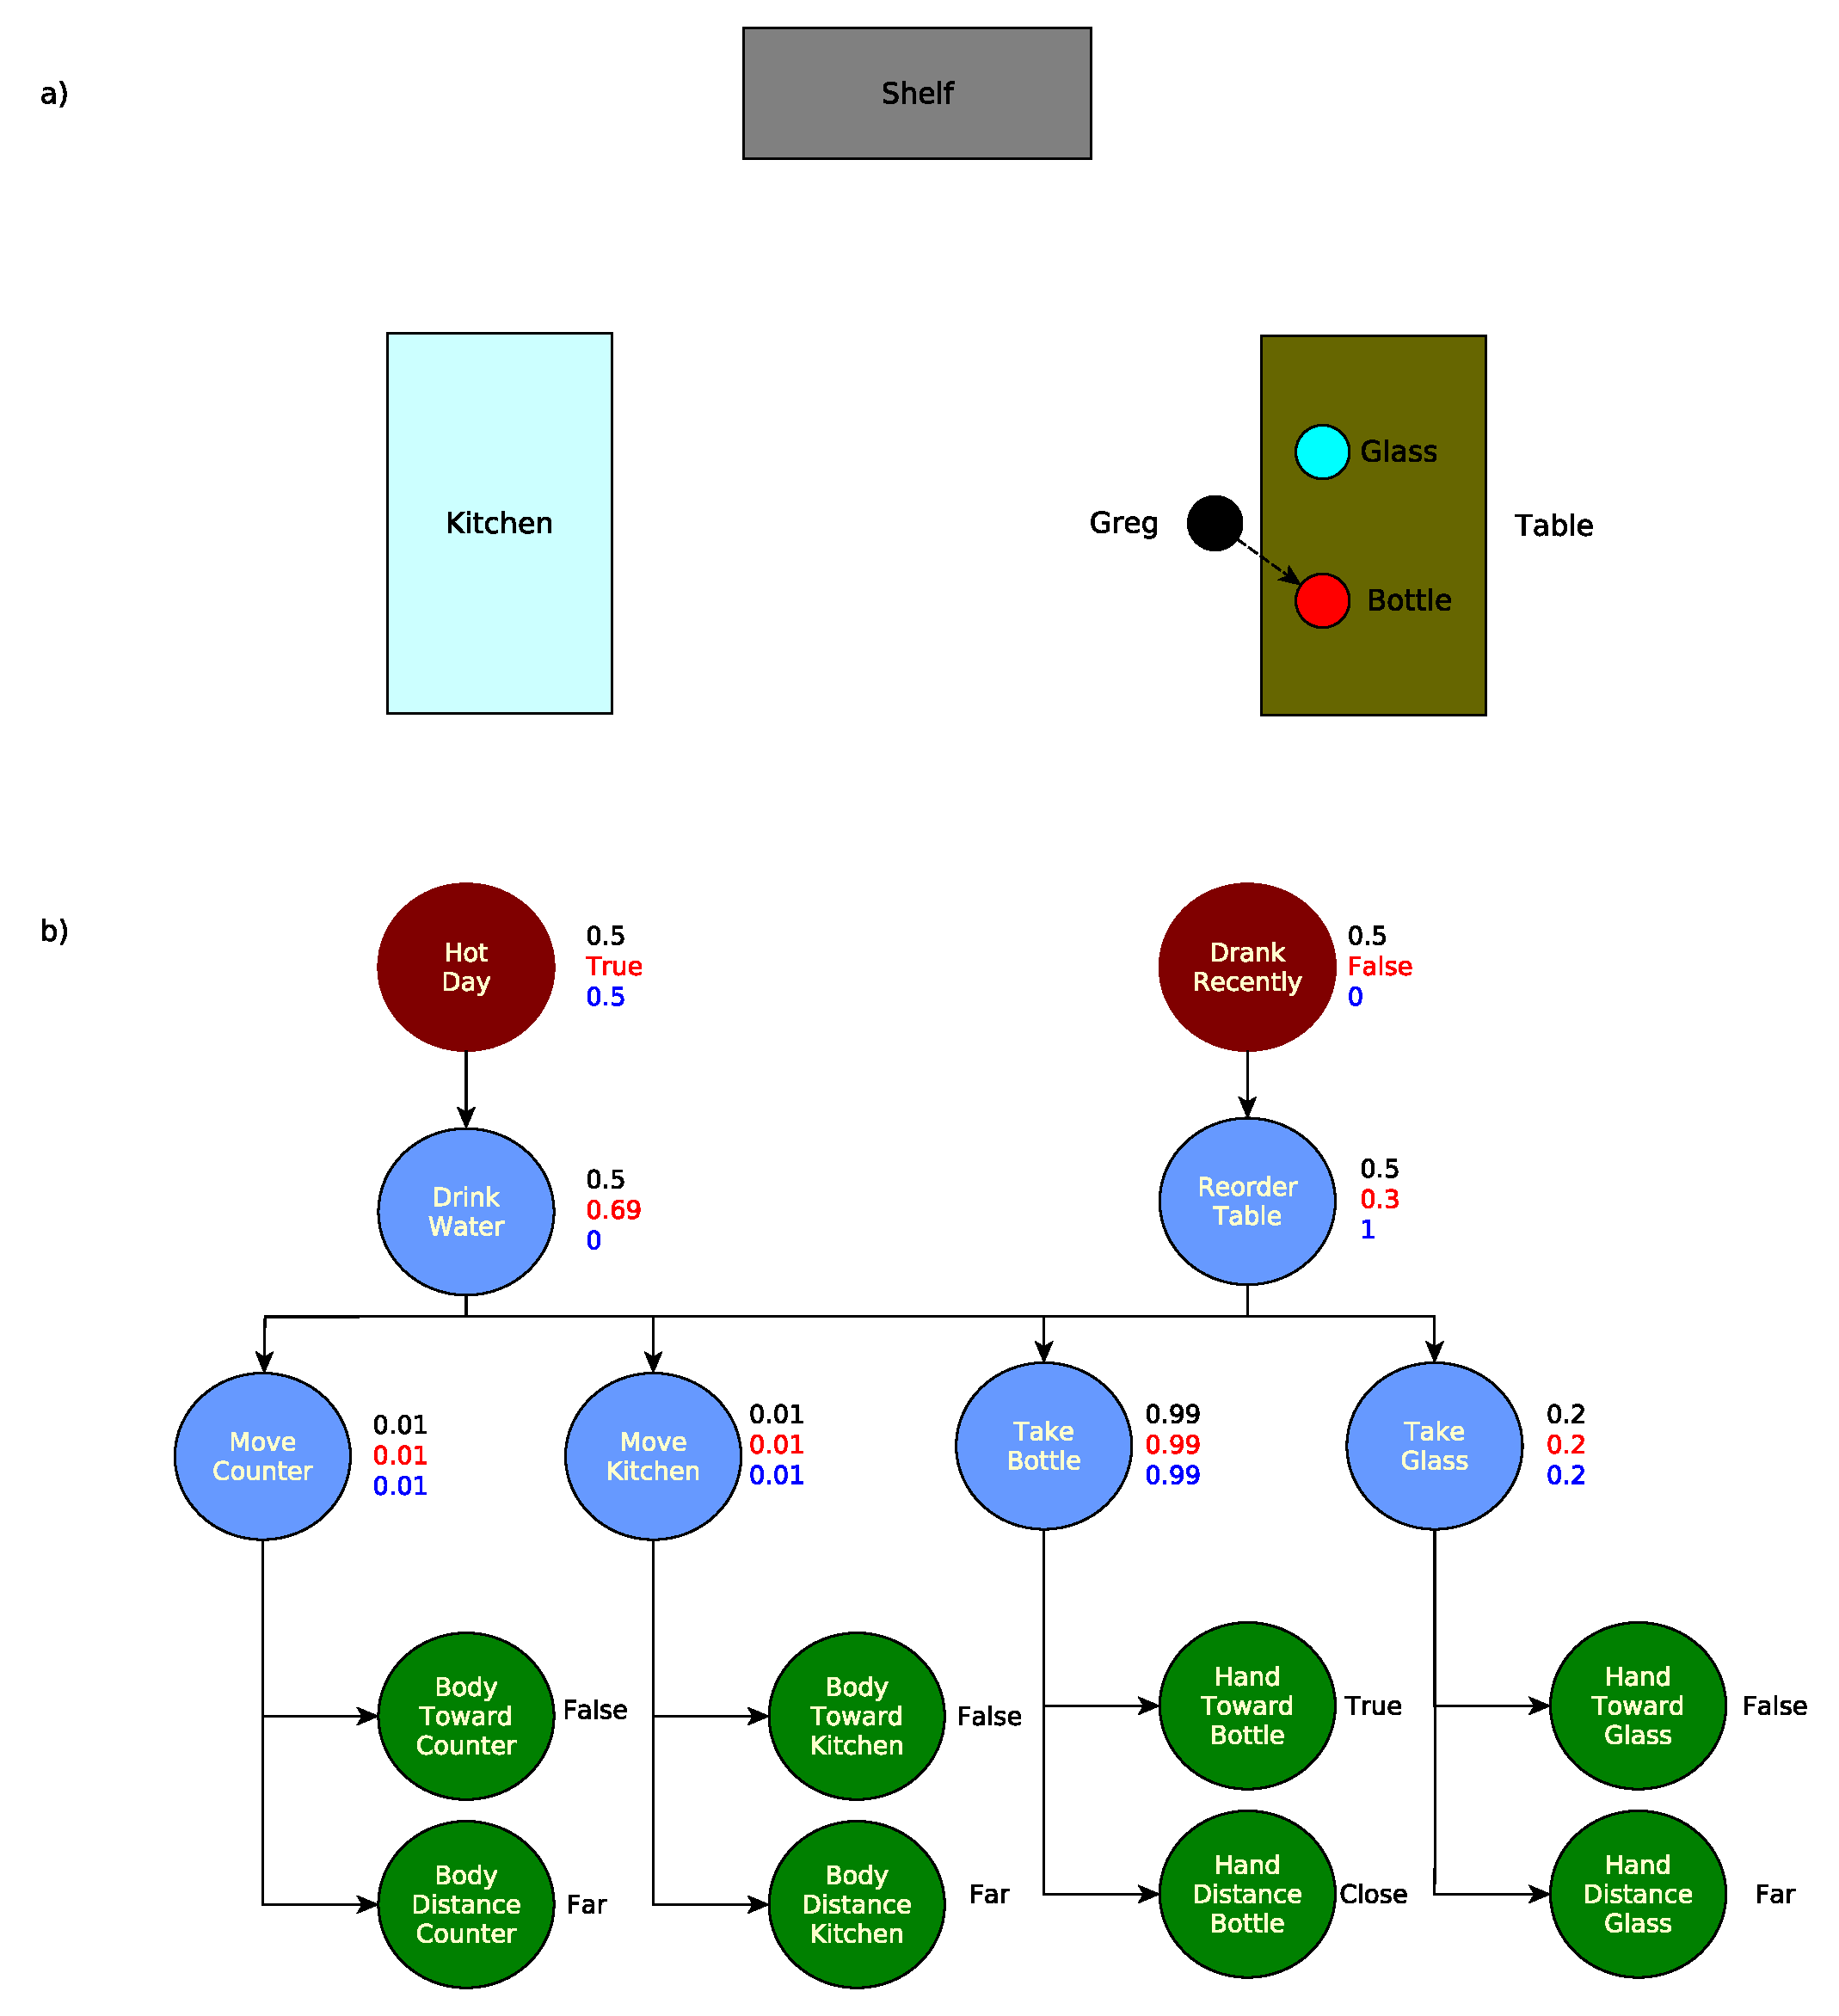
\includegraphics[scale=0.4]{img/situation_assessment/ig_exp2.pdf}
	\caption[IG Example 2]{a) Greg's hand is approaching the bottle. b) The corresponding IG graph. As before, test 1 is shown in black, test 2 in red, and test 3 in blue. The results of 
	the test are very similar to the previous time step, shown in \ref{fig:situation_assessment-ig_exp1}.}
	\label{fig:situation_assessment-ig_exp2}
\end{figure}

\clearpage
 \begin{figure}[ht!]
	\centering
	\includegraphics[scale=0.4]{img/situation_assessment/ig_exp3.pdf}
	\caption[IG Example 3]{a) Greg has taken the bottle, shown by placing the red circle and black circles close. His hand, with the bottle, is now approaching the glass b) The corresponding IG graph. As before, test 1 is shown in black and test 2 in red. Test 3 is not shown since the fill glass action would not be executable in the robot's mental belief model, and so the corresponding IG would be different. In test 1 the system has now sufficient information to infer the corrent intention, which has a value of 0.98. Test 2 confirms this choice.}
	\label{fig:situation_assessment-ig_exp3}
\end{figure}
\clearpage

\subsection{Discussion}

This component is able to estimate the likelihood of a human's intention by combining BNs, MDPs, geometrical reasoning, and the capacity to model human's beliefs. Contextual information can further help to disambiguate the inference process. We will show in the next section that the system is able to approach the capacity of humans to infer intentions. 

Another advantage of our approach is its good scalability. Computing the probabilities in a BN can be done using efficient and well know algorithms, which scale well with the size of the network, meaning that the IG is able to accomodate the addition of new actions, observations and contexts. 

Adding a new intention means creating and solving another MDP. Since this process is done offline this would not impact the run of the system. When computing the conditional probabilities of the action nodes, the system uses the action value function of the MDPs, which is stored in memory and can be directly accessed.
.
\section{Experiments and Discussion}
\label{sec:situation_assessment-experiments}
\subsection{Case Study}
Evaluating the capacity of the system to estimate human intentions is not easy, since intentions are not directly observable. A possible solution, as shown in \cite{baker2014modeling}, is comparing the estimation of human intentions, performed by other humans, with the predictions of our system. In order to perform this comparison we created a user study where we showed participants several videos, asking them to estimate the likelihood of a set of intentions  for each video, and collected their results. The same tests where simulated on a robot, streaming as input a sequence of observations  corresponding to the actions shown in the video (e.g. if the video shows a human approaching the table, we will stream to the robot a trajectory of coordinates that leads to the table position). All of the test videos ended in a situation of ambiguity. For example, in one test we showed a human approaching a table with different objects, and stopped the video before users could see which object the human wanted to take. Some videos include more information than others, like comments by humans or situations that help to disambiguate the intention. 

We have performed an equivalence test, comparing users' intentions predictions with those of the robot, following the two one-sided tests (TOST) approach. We choose as a threshold for equivalence the standard deviation $\sigma$ of the users' answers. The idea behind this choice is that, if the robot's answers are closer than a standard deviation to the average human answers, its predictions are comparable to an average human answer from our user group. 

We defined our hypothesis as follow: 
\begin{itemize}
\item $H_0$: $\mu_{hi}-\mu_{ri}\leq-\sigma_{hi}$ \; \text{OR} \; $\mu_{hi}-\mu_{ri}\geq\sigma_{hi}$ 
\item $H_A$: $-\sigma_{hi}<\mu_{hi}-\mu_{ri}<\sigma_{hi}$  
\end{itemize}
where $\mu_{hi}$ and $\mu_{ri}$ are the human average and the robot's answer for test $i$, $\sigma_{hi}$ is the variance of the human answers for test $i$.

We have performed tests to evaluate: a) prediction in absence of clues, b) prediction in the presence of contextual clues, c) prediction in the presence of belief state clues.

We built a household environment with a fixed set of furniture: a \textit{Kitchen Shelf}, a \textit{Table}, a \textit{Sofa}, and a \textit{Chair}. In this environment, we created two scenarios, composed by several tests, with two agents, \textit{Max} and \textit{Bob}, performing different actions. Each scenario contained a set of objects, and a constrained set of intentions. For the tests related to belief states, we start by showing the users a specific sequence of events, allowing them to build a mental model of the agents. A corresponding simulated sequence will be streamed to the robot for this test.
We will describe in details the two scenarios and the relative tests.

\subsubsection{Cookie Scenario}
\begin{itemize}
\item Objects: a \textit{Cookie Box}, a \textit{Mug}, and a \textit{Bottle of Water} were placed on the \textit{Table}, close to each other. A pack of \textit{Cookies} was placed on the \textit{Kitchen Shelf}. The \textit{Cookie Box} could contain, or not, \textit{Cookies}.
\item Intentions: \textit{Eating a Cookie}, \textit{Drinking Water}, \textit{Reading the Book}.
\item Tests:
\begin{itemize}
	\item \textit{No Clues}: \textit{Max} approaches the \textit{Table}.
    \item \textit{Contextual Clues}: \textit{Max} approaches the \textit{Table} commenting on the warmth of the day.
	\item \textit{Divergent Belief Max}: \textit{Max} approaches the \textit{Table}.
	\item \textit{Divergent Belief Bob}: \textit{Bob} approaches the \textit{Table}.
\end{itemize}
\item  \textit{Divergent Belief Event}:  \textit{Max} and \textit{Bob} are chatting on the \textit{Sofa}. Max eats the last \textit{Cookie} from the \textit{Cookie Box} before closing it and leaving. While \textit{Max} is away, \textit{Bob} takes \textit{Cookies} from the \textit{Kitchen Shelf}, fills the \textit{Cookie Box} with them, and closes it, before leaving.
\end{itemize}

The \textit{Divergent Belief Event} was shown to the users (and its simulation streamed to the robot) between the \textit{Contextual Clues} and the \textit{Divergent Belief Max} events. 


We deliberately included an intention, \textit{Reading the Book}, without placing a book in the visible environment, introducing a confusing element in the scenario. This scenario can be seen in figure~\ref{fig:situation_assessment-cookie}.


 \begin{figure}[ht!]
	\centering
	\includegraphics[scale=0.5]{img/situation_assessment/cookie1-blur.pdf}
	\caption{The cookie intention scenario}
	\label{fig:situation_assessment-cookie}
\end{figure}


\subsubsection{Keys Scenario}
\begin{itemize}
\item Objects: A \textit{Box} was placed on the \textit{Table}, that partially occluded the sight of people approaching. A \textit{Book} and a \textit{Mug} where placed behind the \textit{Box}, so that they could be seen from the sofa but not from approaching people.
\item Intentions: \textit{Taking the Mug}, \textit{Taking the Keys}, \textit{Reading the Book}.
\item Tests and Events:
\begin{itemize}
\item \textit{No Clues}: \textit{Max} approaches the \textit{Table}.
\item\textit{Contextual Clues}: \textit{Max} approaches the \textit{Table} in a hurry, while putting on a coat.
\item \textit{Divergent Belief Max}: \textit{Max} approaches the \textit{Table} in a hurry, while putting on a coat.
\end{itemize}
\item \textit{Divergent Belief Event}: \textit{Max} is sitting on the \textit{Table}, drinking from the \textit{Mug}, while having the \textit{Keys} in his hands. His phone rings, so he drops the \textit{Keys} and the \textit{Mug} on the \textit{Table}, behind the \textit{Box}, and leaves the room. While \textit{Max} is away, \textit{Bob} comes and sits on the \textit{Sofa}, reading a \textit{Book}. When he sees the \textit{Keys}, he takes them, places the \textit{Book} on the \textit{Table}, and leaves.
\end{itemize}

The \textit{Divergent Belief Event} was shown to the users (and its simulation streamed to the robot) between \textit{Contextual Clues} and the \textit{Divegent Belief Max} events. This scenario can be seen in figure~\ref{fig:situation_assessment-keys}

 \begin{figure}[ht!]
	\centering
	\includegraphics[scale=0.5]{img/situation_assessment/keys2-blur.pdf}
	\caption{The keys intention scenario}
	\label{fig:situation_assessment-keys}
\end{figure}

\subsection{User Study}
We built an online user study, where we presented videos related to the tests and events of the two scenarios to users, who had to evaluate the likelihood of each intentions of the scenario
on a five-level Likert scale. The user study was conducted in three languages, with users living in two different countries\footnote{A version of this user study was provided at http://goo.gl/forms/YiuFHnF63c}. We collected answers from 78 adults, performed an average, and converted them to percentile scores, in order to compare them with the robot's predictions.

Looking at users' answers (figure \ref{fig:situation_assessment-user_study_results}), we can see that, in the absence of clues, people rated similarly the two intentions related to visible objects. Contextual clues had the highest influence on users' ratings. This is particularly visible in the \textit{Contextual Clues} test of the \textit{Keys Scenario}, where users chose as the most likely intention \textit{Take Keys}, even if no keys were visible in the video. Divergent beliefs also influenced users decisions, but not as strongly as context. The strongest responses, over all, where given by the \textit{Divergent Belief Max} test on \textit{Keys Scenario}, which uses both divergent belief and contextual information.

\subsection{Robot implementation}
At the start of a scenario the robot scanned the environment, building a model of its world state. With our perception capacities, we can not detect if the cookie box is full or empty, and so we consider it as full at the start of a test, and update its value using the $postconditions$ of inferred human actions. We consider the box as empty when we infer that a human has taken a cookie from inside, and as full when we infer that a human has put a cookie in it.

We have built different IGs for the scenarios. Each test had a different graph, related to its main agent. We considered three different Context Nodes for these IGs: $Hot Day$, true when the day is particularly warm; $Break Time$, true when the agents are taking a pause; $Time to Leave$, true when it's late in the day, and the humans usually leave work and return home.

As previously said, we chose to follow \cite{Liu2014} in order to learn the link between Contexts and Intentions. We created a second user study with 15 users, in which we presented a set of 5 scenarios, each one related to one of the intentions of our tests. For each scenario we asked the users to rate the perceived link, on a five-level Likert scale, between the intention and our three contexts. We averaged users' answers and calculated the conditional probabilities between context nodes and intention nodes from these averages.


In the \textit{Cookie Scenario} the graph for the tests is constructed from the following nodes:
\begin{itemize}
\item Context Nodes: \textit{Hot Day}, \textit{Break Time}, \textit{Time to Leave}
\item Intention Nodes: \textit{Fill Cookie Box}, \textit{Eat Cookie}, \textit{Drink Water}, \textit{Read Book}.
\item Action Nodes: \textit{Move to Table}, \textit{Move to Kitchen}.
\item Observation Nodes: distance of the agent body and hand to each action's associated \textit{target}.
\end{itemize}

We introduce the \textit{Fill Cookie Box} intention, not present in the human test, to allow the robot to detect when Bob fills the \textit{Cookie Box} during the \textit{Divergent Belief Event}.

Our robot does not have speech recognition capacities. We simulated this capacities, and set Context Nodes to plausible values, that could be extracted by watching the videos. For the \textit{Contextual Clues} test, we set the value of \textit{Hot Day} to true (since Max is commenting about the temperature), and \textit{Break Time}, and \textit{Time to Leave} to false (since no data in the video points to one of these contexts being true. Max and Bob seem to have taken a break from work before the other events are shown, in the Divergent Belief Event).
%Our robot doesn't have speech recognition capacities. and for \textit{Contextual Clues} test, set the value of \textit{Hot Day} to \textit{true}, and the value of \textit{Break Time} to \textit{false}, i.e. the robot knows that it is not the usual time for the agents to take a break.

\textit{Divergent Belief Event}, \textit{Divergent Belief Max}, and \textit{Divergent Belief Bob} were showed sequentially to the robot, which updated the agents' mental models and created new IGs accordingly. During the \textit{Divergent Belief Event} several IGs need to be created with different action and observation nodes, to follow the sequence of actions by the two agents. For example, when \textit{Max} leaves the room, \textit{Bob} has the possibility to execute the actions \textit{Take Mug}, \textit{Take Water Bottle}, \textit{Open Cookie Box}, \textit{Move to Kitchen Shelf} or \textit{Leave Room}. Intention and Context nodes remains the same in all the IGs of the scenario.


The \textit{Keys Scenario} has a similar IG, with the following differences.
\begin{itemize}
\item Context Nodes: \textit{Hot Day}, \textit{Break Time} and \textit{Time to Leave}.
\item Intention Nodes: \textit{Drink Water}, \textit{Take Keys}, \textit{Read Book}.
\end{itemize}

Action Nodes and Observation Nodes are the same as the previous scenario, and follow the same ideas during the \textit{Divergent Belief Event}. An example of IG used in the tests can be seen in figure \ref{fig:situation_assessment-intention_graph}. For the \textit{Contextual Clues} and \textit{Divergent Belief} test, we set the \textit{Time to Leave} context value to \textit{true} (since Max is putting a coat and seems in a hurry), and other context node values to \textit{false}. Using the component described in the previous sections, and these IGs the robot was able to obtain predictions from the user actions.

\subsection{Discussion}
\label{sec:discussion}
We performed TOST tests for each intention in the scenarios, comparing the humans' answers with the robot's, for a total of 21 tests. We calculated p-values and performed our tests using a significance value $\alpha=0.05$.

Analyzing the results of our equivalence tests, shown in figure \ref{fig:situation_assessment-user_study_results}, produces some interesting information.
\begin{itemize}
\item The behavior of our system is often close to human capacities. 19 tests out of 21 passed our requirements for significance level, often with very low p-value scores. 
\item Context and Divergent Belief are necessary. A system without these skills would only have been able to model properly the \textit{No Clues} cases. 
\item There are still some missing aspects in our system. We failed to reject the null hypothesis for two tests. In \textit{Divergent Belief Bob} users rated higher the \textit{Eat Cookie} intention than the \textit{Drink Water} intention, possibly because they thought that since \textit{Bob} filled the \textit{Cookie Box} he may want to eat a \textit{Cookie}. This makes us think that humans use deep temporal reasoning to evaluate intentions, considering the whole history of actions performed by agents.  
\end{itemize}
 \begin{figure}[ht!]
	\centering
	\includegraphics[clip,scale=0.5]{img/situation_assessment/pvalues1.pdf}
	\caption[Experiment results]{Experiment results. Results from the two scenarios are represented as graphs. Intentions, as estimated by the humans and the robot, are represented by different colors, as shown in the legend of the graphs, with estimations of the same intention by the robot or the human placed in adjacent position. Each column represents the likelihood of an intention, expressed as a percentile score. P-values from the equivalence tests are shown, linking the estimation of an intention by the humans and by the robot.}
	\label{fig:situation_assessment-user_study_results}
\end{figure}



 

% \part{Case Studies} % Main chapter title

\label{part:case_studies} % Change X to a consecutive number; for referencing this chapter elsewhere, use \ref{ChapterX}

\lhead{Part 1. \emph{Case Studies}} % Change X to a consecutive number; this is for the header on each page - perhaps a


In any application that is not entirely composed by repetitive, precomputed actions, robots need reasoning skills, which severely depend on the quality of the representation of the current environment. This representation can be more or less complex, depending on the application. 

Imagine, for example, a robot whose task is cleaning the floor of a room. In the simplest case, this robot would only be provided with an elementary set of sensors. Without the capacity to understand which areas actually need cleaning, this robot could only move through the room, randomly or with some strategy, achieving the task in a longer amount of time than what would actually be needed. 

% In a fairly simple case, this robot would rely on a map of the room and a set of lasers, or bumper sensors, to detect obstacles. 

Now, imagine a household robot that needs to actively help a family that lives in an apartment, by fetching objects, providing information, and helping to accomplish various tasks. Let us imagine that one of the members of the family, Greg, is moving in the living room, searching around, while exclaming `Where are my glasses?'. In the ideal situation, our robot would try to help Greg, by giving him information such as `They are on the table to your right', or even by fetching them for him. 

Clearly, in this scenario, the robot needs deeper reasoning skills. It needs to understand that the user is looking for its glasses, to link them to their actual physical location, to compute the spatial relationship between the table and the glasses, and to provide information in a natural way. In fact, if the robot would tell Greg that the glasses are in the position $(3.2, 5.0 , 1.3)$, Greg would very likely be very perplexed. A more natural way would be to inform Greg that his glasses are on a table, whose location is pointed taking into account Greg's position.

In this case, having sophisticated sensors is, of course, important but not sufficient. The robot needs also to \textit{reason} on the sensor's data in order to produce meaningful information. For example: laser points and camera images need to be integrated to recognize objects and humans; spatial relationships  (e.g. the glasses are on the table) have to be properly modeled; actions performed by humans, and their effects on the environment, need to be recognized; and so on. 

The process of reasoning on data to produce symbolic information is called \textit{situation assessment}. Endsley explained in \cite{endsley1995toward} that this process is deeply linked to the quality of  decions of the robot.

While in many applications robots can benefit from a situation assessment component, being able to perform complex reasoning on data is particularly important in HRI. If the robot is able to take better decisions (i.e.  efficient, safe, socially acceptable, natural) than it will be perceived in a more positive manner by humans. 




                 % Chapter Template

\chapter{Situation Assessment} % Main chapter title

\label{chap-situation_assessment} % Change X to a consecutive number; for referencing this chapter elsewhere, use \ref{ChapterX}

\lhead{Chapter . \emph{Situation Assessment}} % Change X to a consecutive number; this is for the header on each page - perhaps a shortened title

In this chapter we introduce the Situation Assessment capacities of our system. 

%TODO: Citations on Toaster. Look and add other possible citations. Cite everything. Everything!
\section{Introduction}
\label{sec:situation_assessment-intro}
\subsection{What is Situation Assessment?}
%Motivation
In any application that is not entirely composed by repetitive, precomputed, actions, robots need to possess adeguate reasoning skills, which severely depend on the quality of the representation of their environment. This representation can be more or less complex, depending on the application. Imagine, for example, a robot that needs to clean the floor of a room. For a fairly simple case, this robot would rely on a map of the room and set of lasers, or bumper sensors, to detect and obstacles. Now, imagine a household robot that needs to actively help a family that lives in an apartment, by fetching objects, providing information, and helping accomplish various tasks. Clearly, in this situation, the robot needs a deeper degree of reasoning on sensor data: laser points and camera images need to be integrated to recognize objects and humans; spatial relationships  (e.g. the cup is on the table, the human has the cup) need to be properly modeled; actions performed by humans, and their effects on the environment, need to be recognized; and so on. 

In this situation, there is a need for a process which performs different kinds of reasoning on perceptual data, and produces information that can be used by the rest of the system. This process is called situation assessment, and is deeply linked to the quality of the decisions of the robot, as explained by Endsley in \cite{endsley1995toward}. 


%what are people doing with situation assessment and belief management
Situation assessment components have been designed by different authors, but they are usually developed for specifc applications, like in \cite{Chella2010,Kluge01situationassessment}. In \cite{beetz2015robosherlock}, instead, the authors present ROBOSHERLOCK, an opersource framework that can be used to implement perception systems. Among its features, ROBOSHERLOCK supports logical queries about the world state, and so supporting task-driven situation assessment. 

\subsection{Theory of Mind}
An important part of Situation Assessment is representing other agents in the environment, not as simple obstacles, but as acting entities, with different beliefs on the state of the world, and with the capacity to affect the environment. 

Theory of Mind \cite{premack1978does} is a skill used to reason about humans' beliefs and thoughts, and how they affect actions. An ability linked to this concept is perspective taking, which is widely studied in developmental literature.  Flavell in \cite{flavell1977development} describes two levels of perspective taking: 
1) perceptual perspective taking,  the capacity to understand that other people see the world differently ~\cite{Tversky1999}; and 2) conceptual perspective taking, the capacity to attribute thoughts and feelings to other people ~\cite{Baron1985}. Studies on individuals that don't possess the required mechanisms to perform perspective taking, like young children \cite{frick2014picturing}, have put into light the difficulties these people have to accomplish everyday social relationships and confirmed the importance of this ability.

Previous works in robotics have shown that enhancing the robot's perspective taking abilities improves its reasoning capabilities, leading to more appropriate and efficient task planning and interaction strategies \cite{Trafton2005,ros2010one}. \cite{breazeal2006} showed that perspective taking can even enhance learning by imitation processes, allowing the viewer to learn a task from "flawed" demonstration, which may be correct from the teacher's point of view but are actually ambiguous. 

An important study linked to conceptual perspective taking is the 'divergent belief task'.  Formulated in~\cite{wimmer1983}, this kind of task requires the ability to recognize that others can have beliefs about the world that differ from the observable reality. ~\cite{BreazealGB09} proposed one of the first human-robot implementations, resulting in more advanced goal recognition skills. 

Not many frameworks throughly model different agent's beliefs.  Scheutz \cite{scheutz2013computational}) studied this problem, developing a computation model to represent agent's mental states. The work is oriented in particular toward communication problems and not geometrical and spatial perspective taking issues.

\subsection{Intention Recognition}
%TODO: here in particular we need something for action recognition
Another crucial skill of a robot that interacts with human is recognizing others' actions and goals. Recognizing others' goals is directly linked to modeling humans' beliefs, since, as explained by \cite{byom2013theory} "as humans, we generally believe that others act in ways that are consistent with their beliefs and goals". In psychology \cite{bruner1981} and philosophy \cite{bratman1984} literature, an intention as the wish and will to achieve a goal. Intentions memerge from contextual causes (motivations) and are present the goal is achieved or abandoned, pushing agents to undertake actions leading to that goal.

The recognition of human activities is an important topic in computer science research, which can be studied at different levels. Anticipating human actions and movements allows the robot to adapt its behavior and proactively help humans, as studied in \cite{koppula2013anticipating}. An interesting idea is using the robot's own internal models in order to recognize actions and predict user intents, as shown by the \textit{HAMMER} system in \cite{demiris2007prediction}. Sequences of actions can be linked to plans, a well-known topic called plan recognition. Several approaches have been studied in this domain using, for example, classical planning \cite{ramirez2009plan}, probabilistic \cite{bui2003general} or logic techniques \cite{singla2011abductive}.  In \cite{talamadupula2014coordination}, the authors use classical planning, with an efficient replanning strategy, in order to infer user's intentions. The system has been implemented on a PR2 robot and tested on a collaborative scenario. \cite{breazeal2009embodied} presents an architecture in which the robot is able to use its own schemas and models to infer human actions and goals, and to proactively help him achieve them. Shared plans are not explicitly represented in the system, and the robot helps the human by mapping the inferred goal information in its own beliefs, and choosing appropriate action

Two approaches that can be used for intention estimation are Interactive Partially Observed Markov Decision Processes (I-POMDP) and Inverse Learning. I-POMDP  \cite{gmytrasiewicz2004interactive} offer a rich framework that extends Partially Observed Markov Decision Processes (POMDP) in a multi-agent setting. Inference in these models can be extremely complex, but there have been attempts at solving this issue, like in \cite{doshi2009monte,hoang2013interactive}. 

Inverse Reinforcement Learning \cite{ng2000algorithms} formulates the problem of computing an unknown reward function of an agent after observing his behavior. This strategy has been applied, with Bayesian Networks (BN), in \cite{Nagai2015}, in order to learn the mental model of another agent, and choose appropriate actions for a relationship building task. A linked approach is inverted planning, which has been applied in a bayesian framework in \cite{baker2009action}  for human action understanding.

Contextual information can be used to further disambiguate complex situations. \cite{Liu2014} shows a system using BNs to understand users' intentions with an emphasis on contextual information.

It is very important to consider humans' beliefs when estimating their intentions. In a dynamic environment, agents can execute actions, modifying the state of the world without other agents being able to perceive the changes. Let us imagine a scenario. Bob comes back home from work and would like to relax while reading. He lays down on a sofa with a book, and reaches to a nearby table to grab his glasses. He does not know that his wife, during the day, moved the glasses to another room. If we would ignore Bob's beliefs on the world (i.e. he does not know that the glasses are not on the table) we could infer that, for example, Bob would like a drink while he is sitting on the sofa, or the tv remote controller. If, instead, we would know that Bob thinks his glasses are on the table (and we would use other contextual information perhaps, like Bob's habitudes) we would be able to correctly infer Bob's current intention, that is, taking his glasses, and warn him that they are not there, perhaps even fetching them for him. In robotics, an interesting framework that considers this issue is the Bayesian Theory of Mind \cite{baker2014modeling}, used to represent the inference process of an observer looking at another agent's behaviors, with POMDPs and Dynamic Bayesian Networks (DBNs).


\subsection{Dialogue}
Dialogue is a very important part of situation assessment. Agents often communicate, while executing a task together, or even when working independently, to clarify ambiguities and obtain missing information. While we will not present a specific dialogue component in this work, we have used our system in \cite{Ferreira2015}, where our belief management component and a situated dialogue system were implemented in a simulator. This model was compared with a basic system (without belief awareness) in a study with 60 interactions, in a simulated environment. We successfully showed that the dialogue management system significantly improves its efficiency, reducing the number of dialogue turns in the interaction, and its accuracy, with a higher success rate when a divergent belief situation appears.

\section{System Overview}
\label{sec:situation_assessment-overview}

In our architecture, we built a Situation Assessment layer, which is able to:
\begin{itemize}
\item  Detect and track entities.
\item  Process sensor data in order to produce symbolic information.
\item  Maintain a belief model for each agent.
\item  Infer human actions and intentions. Our system is able to perform this estimation by taking into account the current belief of humans on the world state. 
\end{itemize} 

This layer is composed by different elements, as shown in Fig. \ref{fig:situation_assessment-situation_assessment_overview}.
\begin{itemize}
\item Sensor Data. Data produced by different possible sensors (e.g. lasers, camera, etc.)
\item Entity Detection. Different components detect and track humans and objects in the environment.
\item Human Inputs. Users can communicate with the robot by using a tablet application.
\item Human Interface. User inputs from the tablet are elaborated into commands, to introduced in the Database.
\item Geometrical Reasoning. Symbolic facts are produced starting from perceptual data.
\item Belief Management. The system maintains a mental model of each agent.
\item Intention and Action Recognition. Human actions and intentions are inferred based information provided by the Geometrical Reasoning and on the belief models of the agents.
\item Database. The database stores symbolic facts produced by the system.
\end{itemize}


 \begin{figure}[h!]
	\centering
	\includegraphics[scale=0.45]{img/situation_assessment/situation_assessment_overview}
	\caption{Overview of the different modules composing the Situation Assessment Layer}
	\label{fig:situation_assessment-situation_assessment_overview}
\end{figure}


In addition, the system possesses a description of the world, with a definition of all the elements known to the robot, like objects and agents, possible actions, possible intentions, intentions, etc. 
Symbolic facts are constantly produced starting from the sensor data and from the position of entities, and then the Belief Manager will update and maintain the belief model of each agent. The belief model of humans and of the robot will be used by the Intention and Action Recognition modules to infer the most likely intentions and actions performed. All these information are introduced in the Database, and can be read by other components. For example, the Goal Manager can choose a goal based on human commands or on an estimation of its intention. In a similar way, the Action Execution modules will read the Database in order to obtain the state of the world, to check action preconditions.  

Our situation assessment layer was presented in \cite{Milliez2014}, where it was used to pass the Sally and Anne test~\cite{Baron1985} on a robotic platform. The intention and action recognition capacity was introduced in \cite{devin2016some}.

\section{Object and Human Detection}
In our system, we chose to simplify perception issues, focusing on reasoning aspects. We associate a unique tag to every object that is interesting in a particular scenario.  When the robot observes a tag using a camera, it detects the corresponding object using a tag-matching algorithm.
Regarding humans, we use a motion capture software to identify and track agents moving in the environment. Using different tags, we can track the head, shoulders, and right arm of a human. Our situation assessment component has also been tested using a laser and RGB based detector in the SPENCER european project \footnote{http://www.spencer.eu/}.

\section{Human-Robot Communication}
Similarly, communication between the human and the robot is limited, in our system. Humans can give commands to the robot by using a tablet application, where they can manage the robot goals, by adding a new goal, canceling a previous one, or pausing the robot. The robot is able to provide simple verbal output by using a text-to-speech component. The robot is not able to perform real dialogues with the human but it can adapt its speech to the current tasks and scenarios, by explaining plans, informing the human if it has a problem, verbalizing its current actions, and so on. This feature will be explained fully in chapter \ref{chap-plan production and management}. 

\section{World Model and Geometrical Reasoning}
\label{sec:situation_assessment-situation_assessment}
The first step in estimating human intentions is reasoning about the environment and the belief of humans. Our world is composed by agents, the robot and humans; by objects; and by areas, which are bounded regions in the environment with semantic meaning, e.g. living room, kitchen. To be more generic, we will sometimes use the word \textit{entity} to refer to an agent, an agent's joint or an object. We can assign properties, to entities and areas to represent different information, e.g. 
an agent can be in a specific area, a box can be opened and can contain objects, a bottle can contain liquids, a mug can be hot. The $subject$ of a property is the name of the primary entity linked to it (e.g. bob, mug). 
 We divide properties in two classes: 
\begin{itemize}
\item fully observable:  can be seen by any present agent looking at the linked entity or area, e.g. the box is open
\item partially observable: can be observed by present agents only in specific situations, represented as rules linked to the object and the property, e.g. an agent can see that a box contains items only when it is open, an agent can detect that the mug is hot only when he touches it.
\end{itemize}

Using its perception abilities the robot can build a representation of the environment, starting with entities' positions. Using geometrical reasoning we can compute spatial relationships between entities, e.g. the glasses are on the shelf, the human is moving toward the library, the glasses are reachable by the human, the bottle is visible for the human. These reasonings provide a base for the perspective taking abilities of the robot. 


\section{Belief Management}
\label{sec:situation_assessment-belief_management}
In our system, agents can have divergent representations of the world. To model this aspect, the information produced by perception, geometrical reasoning and inference, are collected by the robot in \textit{belief models}, built for itself and for each agent. A \textit{belief model} is a symbolic representation of the world state, as known by an agent. In a model, the world state is represented by properties and values. To represent the lack of knowledge of an agent, the value of a property can be \textit{unknown}.

We consider our world as a dynamic environment, where properties can change and actions can be performed.  We define an action as a tuple $(name, preconditions, target, postconditions)$. The $name$ of an action is a unique string that identifies it. The $preconditions$ are a list of properties that must be true in order to realize the action. In our system, an action is executed on a $target$, which can be a physical object, like a cup, but also an area of the environment, like a room. The $postconditions$ are the set of properties, and their values, affected by the action's execution.

Since we are interested on reasoning and not perceptual aspects, we use inference, as explained in Sec. \ref{sec:situation_assessment-intention_recognition}, in order to understand when a human has performed an action. Through the predefined $postconditions$ of actions we can also infer changes in object properties, e.g. the human opens a box, so the box is now open. 

We created a rule based framework in order to build the beliefs of each agent and update them when needed. Human belief models are updated using the perspective taking skills of the robot. When the robot detects the execution of an action in the world, it updates the belief model for itself and for every human that can perceive the action, adding the action's $postconditions$ to their models. When an action is not perceived by a human (e.g. the user was in an other room), his belief model will not be updated, as he is not aware of the changes that occurred.

However, when he comes back and looks at the environment, we assign him a new belief state following a set of rules, which we will now explain. We call $H$ the agent, $HB$ his belief model, and $RB$ the robot's belief model. We also create the following predicates: $obs(p)$ means that the instance of property $p$ is observable, $valid(p,x)$ means that the instance of property $p$ doesn't contradict the current perception data of agent $x$, $value(p,m)$ is the value of predicate $p$ in belief model $m$, and $vis(p,x)$ means that agent $x$ has visibility on the linked entities of property $p$. The rules for the $valid$ predicate will be different in each property. For example the property \textit{MUG isOn TABLE} won't be valid for agent Max if he can see that there is no mug on the table. For each property $p\in HB \cup RB$:
\begin{itemize}
\item if $p \in RB, \quad p\not\in HB,\quad obs(p),\quad vis(p,H) \rightarrow value(p,HB)=value(p,RB)$.
\item if $p \not \in RB,\quad p\in HB,\quad obs(p),\quad vis(p,H) \rightarrow remove\quad $p$ \quad from \quad HB$.
\item if $p\in RB,\quad p\in HB$ then:
	\begin{itemize}
      \item if $value(p,HB)\neq value(p,RB),\\ \quad obs(p),\quad vis(p,H) \rightarrow \\ value(p,HB)=value(p,RB)$.
      \item if $value(p,HB)\neq value(p,RB),\\ \quad !obs(p),\quad !valid(p,H) \rightarrow \\ value(p,HB)=\textit{unknown}$.
	\end{itemize}
\end{itemize}
The idea of this set of rules is updating an agent's mental belief model for a property only if it's observable, or if it's not observable and perception data contradicts the current value of the property (e.g. the mug was moved from the table to the kitchen while the agent was in another room: while the agent can not see where is the mug, he can see it is no longer on the table).



\section{Action and Intention Inference}
\label{sec:situation_assessment-intention_recognition}

In order to infer human intentions, we will provide the following information to the robot: a list of known contexts, a list of known intentions, a list of known actions, a set of observations of human actions, and a belief model of humans and of itself.

We propose, as central model used for intention estimation, a framework based on BNs. We call our implementation of BN an Intention Graph (IG).
An IG is linked to a specific agent, and composed by the following layers of nodes:
\begin{itemize}
\item Context Nodes: these nodes represent contextual information, modeled as boolean variables (e.g. HotDay, ColdDay).
\item Intention Nodes: these boolean nodes represent the set of possible intentions. Each intention can conditionally depend on several contexts.
\item Action Nodes. This is the set of human actions whose preconditions . Each of these nodes is conditionally dependent on all the intention nodes. 
\item Observation Nodes. We associate to each action a different set of observation nodes, that depend conditionally on the associated action node. 
\end{itemize}

In a typical usage, the robot will create, for each monitored human, an IG, formed by the Context and Intention Nodes, which we consider statically known by the robot, and a variable list of Action and Observation nodes, which depends on the human's belief model. The robot will create action nodes for each known action whose $preconditions$ are satisfied in the human's belief model, and their related Observation Nodes. These IGs will need to be updated every time that an agent performs an action, switching the previous Action and Observation nodes with new ones, that will depend on the state of the world after the action was performed.

When monitoring a human, we set Context Nodes and Observation Nodes as \textit{evidence}, considering them observable by the robot. These information will allow us to have a good estimation of the most likely actions and intentions of the human, as explained in \ref{intention and action inference}.

An example of IG, taken from an experiment, can be seen in figure \ref{fig:situation_assessment-intention_graph}. In the following paragraphs, we will explain the role of these layers of nodes, and how the conditional dependencies between them are computed.

 \begin{figure}[h!]
	\centering
	\includegraphics[trim={2cm 11cm 11cm 17cm},clip,scale=0.45]{img/situation_assessment/cookieScenario.pdf}
	\caption{A scene from our experiment. The yellow arrows show possible actions and their associated probabilities. The diagram represents the current IG. Green circles represent evidence nodes and blue circles other nodes. For the Context Nodes (top of the graph), we represented nodes with a false value as greyed out, and nodes with a true value as green. The most likely nodes in the graph are represented with a glowing effect. The observation nodes where compressed in a single block to simplify the diagram}
	\label{fig:situation_assessment-intention_graph}
\end{figure}

\subsection{From Contexts to Intentions}
We introduce a set of contexts in our domain. We consider as context any information that can be used to characterize and motivate an intention \cite{abowd1999towards}. We model a context  as a property, which can assume different values and influences the probability of a user having a particular intention. For example, we imagine that a human is more likely to be cooking at dinner time, or to drink a hot mug of tea on a cold day.

Contextual nodes can directly influence one or more Intention nodes. In this work, we chose to learn these conditional dependencies from humans, as explained in section \ref{situation_assessment-experiments}.

\subsection{From Intentions to Actions}
\label{sec:situation_assessment-action_evaluation}
To understand how actions are linked to intentions the robot needs to answer the following question: what actions would a human take, in this situation, given his belief of the world, in order to achieve its intention?
Our idea is based on the principle of rationality \cite{Dennet1989}, which states that agents tend to choose the most efficient actions, taking into account their beliefs about the world, in order to achieve their desires.

In \cite{Blakemore2001}, the authors explain that "the attribution of intentions to actions might rely on simulating the observed action and mapping it into representations of our own intention". We represent this idea by providing the robot with a set of planning models. Each one of these planning models is related to an intention, and represents all the known plans to achieve its linked goal. In this way, we can estimate how much the current human actions are compatible with the plans related to an intention.

In our implementation, for each intention known by the robot, we will create an associated Markov Decision Process (MDP), to represent all the possible plans associated to this intention. After solving the set of MDPs we will use the calculated action value function \(Q(s,a)\), to create conditional dependencies between Intention and Action nodes in the IG. Let's start by defining \(P(a|I_i=1)\), the probability that action $a$ will be performed if intention $I_i$ is true. We model this probability as \(P(a|I_i=1)=\frac{Q_i(s,a)}{\sum_b(Q_i(s,b))}\), where we normalize the value function $Q_i(s,a)$ for intention $i$ and action $a$ in the human's belief state $s$, over the value function $Q_i(s,b)$ calculated on all the monitored actions $b$. We can extend this calculation to the case where a generic number of intentions are true to compute the probabilities of action nodes: \(P(a|I_1,I_2,...,I_m)=\frac{\sum_{i:I_i=1}Q_i(s,a)}{\sum_b\sum_{i:I_i=1}Q_i(s,b)}\).

The key idea in this problem is to use the human's belief state as input for the MDPs' value functions. In this way we are using perspective taking at a planning level as the human action is consistent with his intention in his own belief state but may be irrelevant in the real world (e.g. in case of wrong belief).

Our idea is similar to \cite{karami2010human}, where human intentions are estimated using a POMDP and a set of MDPs, that simulate human policies related to different intentions. In this work we use a BN instead of a POMDP, which allows us to separate the mechanisms used for inference and for the robot's actions. Also, we improve the recognition process by including the belief state of the human.

\subsection{From Actions to Observations}
Intentions will be inferred from human actions, so the robot needs to monitor their execution. For each Action Node we define a set of four Observations Nodes: the distance of the human's body from the action's $target$, its variation, the distance of the human's hand from the action's $target$, and its variation. The conditional dependencies of the Observation Nodes are precomputed.

\subsection{Intention and Action Inference}
\label{sec:situation_assessment-intention and action inference}
We assume, in this work, that at each moment a human can only execute a single action, and the robot will react only on his most likely intention. The most likely action and intention are inferred from the BN in the following way. We call $P(n)$ the inferred probability of a node $n$, $B(n)$ the set of brothers of $n$ (that is, nodes on the same layer), and $\delta_1$, $\delta_2$ two thresholds. The robot infers that an action has been realized, or that a human has an intention following these rules: 
\begin{itemize}
\item  \(P(n_i)>\delta_1\) 
\item  \(\forall b \in B(n_i): P(n_i)>P(b)+\delta_2\), where $n_i$ is the node associated to the interested intention or action.
\end{itemize}

When the robot infers that an action has been performed, it updates the world state with its $postconditions$, triggering an update on the beliefs of all present agents. The current human intention is recorded in the Database, in order to be used by the Goal Manager.


\section{Experiments and Discussion}
\label{sec:situation_assessment-experiments}
\subsection{Case Study}
Evaluating the capacity of the system to estimate human intentions is not easy, since intentions are not directly observable. A possible solution, as shown in \cite{baker2014modeling}, is comparing the estimation of human intentions, performed by other humans, with the predictions of our system. In order to perform this comparison we created a user study where we showed participants several videos, asking them to estimate the likelihood of a set of intentions for each video, and collected their results. 

We performed an equivalence test, comparing users' intentions predictions with those of the robot, following the two one-sided tests (TOST) approach. We choose as a threshold for equivalence the standard deviation $\sigma$ of the users' answers. The idea behind this choice is that, if the robot's answers are closer than a standard deviation to the average human answers, its predictions are comparable to an average human answer from our user group. 

We defined our hypothesis as follow: 
\begin{itemize}
\item $H_0$: $\mu_{hi}-\mu_{ri}\leq-\sigma_{hi}$ OR $\mu_{hi}-\mu_{ri}\geq\sigma_{hi}$ 
\item $H_A$: $-\sigma_{hi}<\mu_{hi}-\mu_{ri}<\sigma_{hi}$  
\end{itemize}
where $\mu_{hi}$ and $\mu_{ri}$ are the human average and the robot's answer for test $i$, $\sigma_{hi}$ is the variance of the human answers for test $i$.

We performed tests to evaluate: a) prediction in absence of clues, b) prediction in the presence of contextual clues, c) prediction in the presence of belief state clues.

We built a household environment with a fixed set of furniture: a \textit{Kitchen Shelf}, a \textit{Table}, a \textit{Sofa}, and a \textit{Chair}. In this environment, we created two scenarios, composed by several tests, with two agents, \textit{Max} and \textit{Bob}, performing different actions. Each scenario contained a set of objects, and a constrained set of intentions. For the tests related to belief states, we start by showing the users and the robot a specific sequence of events, allowing them to build a mental model of the agents. We will describe in details the two scenarios and the relative tests.

\subsubsection{Cookie Scenario}
\begin{itemize}
\item Objects: a \textit{Cookie Box}, a \textit{Mug}, and a \textit{Bottle of Water} were placed on the \textit{Table}, close to each other. A pack of \textit{Cookies} was placed on the \textit{Kitchen Shelf}. The \textit{Cookie Box} could contain, or not, \textit{Cookies}.
\item Intentions: \textit{Eating a Cookie}, \textit{Drinking Water}, \textit{Reading the Book}.
\item Tests:
\begin{itemize}
	\item \textit{No Clues}: \textit{Max} approaches the \textit{Table}.
    \item \textit{Contextual Clues}: \textit{Max} approaches the \textit{Table} commenting on the warmth of the day.
	\item \textit{Divergent Belief Max}: \textit{Max} approaches the \textit{Table}.
	\item \textit{Divergent Belief Bob}: \textit{Bob} approaches the \textit{Table}.
\end{itemize}
\item  \textit{Divergent Belief Event}:  \textit{Max} and \textit{Bob} are chatting on the \textit{Sofa}. Max eats the last \textit{Cookie} from the \textit{Cookie Box} before closing it and leaving. While \textit{Max} is away, \textit{Bob} takes \textit{Cookies} from the \textit{Kitchen Shelf}, fills the \textit{Cookie Box} with them, and closes it, before leaving.
\end{itemize}

The \textit{Divergent Belief Event} was shown to the users and the robot between the \textit{Contextual Clues} and the \textit{Divergent Belief Max} events. 

We deliberately included an intention, \textit{Reading the Book}, without placing a book in the visible environment, introducing a confusing element in the scenario.

\subsubsection{Keys Scenario}
\begin{itemize}
\item Objects: A \textit{Box} was placed on the \textit{Table}, that partially occluded the sight of people approaching. A \textit{Book} and a \textit{Mug} where placed behind the \textit{Box}, so that they could be seen from the sofa but not from approaching people.
\item Intentions: \textit{Taking the Mug}, \textit{Taking the Keys}, \textit{Reading the Book}.
\item Tests and Events:
\begin{itemize}
\item \textit{No Clues}: \textit{Max} approaches the \textit{Table}.
\item\textit{Contextual Clues}: \textit{Max} approaches the \textit{Table} in a hurry, while putting on a coat.
\item \textit{Divergent Belief Max}: \textit{Max} approaches the \textit{Table} in a hurry, while putting on a coat.
\end{itemize}
\item \textit{Divergent Belief Event}: \textit{Max} is sitting on the \textit{Table}, drinking from the \textit{Mug}, while having the \textit{Keys} in his hands. His phone rings, so he drops the \textit{Keys} and the \textit{Mug} on the \textit{Table}, behind the \textit{Box}, and leaves the room. While \textit{Max} is away, \textit{Bob} comes and sits on the \textit{Sofa}, reading a \textit{Book}. When he sees the \textit{Keys}, he takes them, places the \textit{Book} on the \textit{Table}, and leaves.
\end{itemize}

The \textit{Divergent Belief Event} was shown to the users and the robot between \textit{Contextual Clues} and the \textit{Divegent Belief Max} events.

\subsection{User Study}
We built an online user study, where we presented videos related to the tests and events of the two scenarios to users, who had to evaluate the likelihood of each intentions of the scenario
on a five-level Likert scale. The user study was conducted in three languages, with users living in two different countries\footnote{A version of this user study was provided at http://goo.gl/forms/YiuFHnF63c}. We collected answers from 78 adults, performed an average, and converted them to percentile scores, in order to compare them with the robot's predictions.

Looking at users' answers (Fig. \ref{fig:situation_assessment-user_study_results}), we can see that, in the absence of clues, people rated similarly the two intentions related to visible objects. Contextual clues had the highest influence on users' ratings. This is particularly visible in the \textit{Contextual Clues} test of the \textit{Keys Scenario}, where users chose as the most likely intention \textit{Take Keys}, even if no keys were visible in the video. Divergent beliefs also influenced users decisions, but not as strongly as context. The strongest responses, over all, where given by the \textit{Divergent Belief Max} test on \textit{Keys Scenario}, which uses both divergent belief and contextual information.

\subsection{Robot implementation}
At the start of a scenario the robot scanned the environment, building a model of its world state. With our perception capacities, we can't detect if the cookie box is full or empty, and so we consider it as full at the start of a test, and update its value using the $postconditions$ of inferred human actions. We consider the box as empty when we infer that a human has taken a cookie from inside, and as full when we infer that a human has put a cookie in it.

We built different IGs for the scenarios. Each test had a different graph, related to it's main agent. We considered three different Context Nodes for these IGs: Hot Day, true when the day is particularly warm; Break Time, true when the agents are taking a pause; Time to Leave, true when it's late in the day, and the humans usually leave work and return home.

As previously said, we chose to follow \cite{Liu2014} in order to learn the link between Contexts and Intentions. We created a second user study with 15 users, in which we presented a set of 5 scenarios, each one related to one of the intentions of our tests. For each scenario we asked the users to rate the perceived link, on a five-level Likert scale, between the intention and our three contexts. We averaged users' answers and calculated the conditional probabilities between context nodes and intention nodes from these averages.


In the \textit{Cookie Scenario} the graph for the tests is constructed from the following nodes:
\begin{itemize}
\item Context Nodes: \textit{Hot Day}, \textit{Break Time}, \textit{Time to Leave}
\item Intention Nodes: \textit{Fill Cookie Box}, \textit{Eat Cookie}, \textit{Drink Water}, \textit{Read Book}.
\item Action Nodes: \textit{Move to Table}, \textit{Move to Kitchen}.
\item Observation Nodes: distance of the agent body and hand to each action's associated \textit{interesting points}.
\end{itemize}

We introduce the \textit{Fill Cookie Box} intention, not present in the human test, to allow the robot to detect when Bob fills the \textit{Cookie Box} during the \textit{Divergent Belief Event}.

Our robot doesn't have speech recognition capacities. We simulated this capacities, and set Context Nodes to plausible values, that could be extracted by watching the videos. For the \textit{Contextual Clues} test, we set the value of \textit{Hot Day} to true (since Max is commenting about the temperature), and \textit{Break Time}, and \textit{Time to Leave} to false (since no data in the video points to one of these contexts being true. Max and Bob seem to have taken a break from work before the other events are shown, in the Divergent Belief Event).
%Our robot doesn't have speech recognition capacities. and for \textit{Contextual Clues} test, set the value of \textit{Hot Day} to \textit{true}, and the value of \textit{Break Time} to \textit{false}, i.e. the robot knows that it is not the usual time for the agents to take a break.

\textit{Divergent Belief Event}, \textit{Divergent Belief Max}, and \textit{Divergent Belief Bob} were showed sequentially to the robot, which updated the agents' mental models and created new IGs accordingly. During the \textit{Divergent Belief Event} several IGs need to be created with different action and observation nodes, to follow the sequence of actions by the two agents. For example, when \textit{Max} leaves the room, \textit{Bob} has the possibility to execute the actions \textit{Take Mug}, \textit{Take Water Bottle}, \textit{Open Cookie Box}, \textit{Move to Kitchen Shelf} or \textit{Leave Room}. Intention and Context nodes remains the same in all the IGs of the scenario.


The \textit{Keys Scenario} has a similar IG, with the following differences.
\begin{itemize}
\item Context Nodes: \textit{Hot Day}, \textit{Break Time} and \textit{Time to Leave}.
\item Intention Nodes: \textit{Drink Water}, \textit{Take Keys}, \textit{Read Book}.
\end{itemize}

Action Nodes and Observation Nodes are the same as the previous scenario, and follow the same ideas during the \textit{Divergent Belief Event}. An example of IG used in the tests can be seen in Fig. \ref{fig:situation_assessment-intention_graph}. For the \textit{Contextual Clues} and \textit{Divergent Belief} test, we set the \textit{Time to Leave} context value to \textit{true} (since Max is putting a coat and seems in a hurry), and other context node values to \textit{false}. Using the component described in the previous sections, and these IGs the robot was able to obtain predictions from the user actions.

\subsection{Discussion}
\label{sec:discussion}
We performed TOST tests for each intention in the scenarios, comparing the humans' answers with the robot's, for a total of 21 tests.

We calculated p-values and performed our tests using a significance value $\alpha=0.05$.

Analyzing the results of our equivalence tests, shown in Fig. \ref{fig:situation_assessment-user_study_results}, produces some interesting information. 1) The behavior of our system is often close to human capacities. 19 tests out of 21 passed our requirements for significance level, often with very low p-value scores. 2) Context and Divergent Belief are necessary. A system without these skills would only have been able to model properly the \textit{No Clues} cases. 3) There are still some missing aspects in our system. We failed to reject the null hypothesis for two tests. In \textit{Divergent Belief Bob} users rated higher the \textit{Eat Cookie} intention than the \textit{Drink Water} intention, possibly because they thought that since \textit{Bob} filled the \textit{Cookie Box} he may want to eat a \textit{Cookie}. This makes us think that humans use deep temporal reasoning to evaluate intentions, considering the whole history of actions performed by agents.  

 \begin{figure}[h!]
	\centering
	\includegraphics[clip,scale=0.32]{img/situation_assessment/pvalues1.pdf}
	\caption{Experiment results. Results from the two scenarios are represented as graphs. Intentions, as estimated by the humans and the robot, are represented by different colors, as shown in the legend of the graphs, with estimations of the same intention by the robot or the human placed in adjacent position. Each column represents the likelihood of an intention, expressed as a percentile score. P-values from the equivalence tests are shown, linking the estimation of an intention by the humans and by the robot.}
	\label{fig:situation_assessment-user_study_results}
\end{figure}



 
\chapter{Inferring Human Intention and Reacting} % Main chapter title

\label{chapter:intention} % Change X to a consecutive number; for referencing this chapter elsewhere, use \ref{ChapterX}

\lhead{Chapter 3. \emph{Intention Recognition}} % Change X to a consecutive number; this is for the header on each page - perhaps a shortened title


\section{Introduction}
Another crucial skill to interact with humans is recognizing others' actions and goals. This process is is directly linked to modeling humans' beliefs, since, as explained by \cite{byom2013theory} ``as humans, we generally believe that others act in ways that are consistent with their beliefs and goals". 

The recognition of human activities is an important topic in computer science research, which can be studied at different levels. Anticipating human actions and movements allows the robot to adapt its behavior and proactively help humans, as studied in \cite{koppula2013anticipating}. 

Sequences of actions can be linked to plans, a well-known topic called plan recognition. Several approaches have been studied in this domain using, for example, classical planning \cite{ramirez2009plan}, probabilistic \cite{bui2003general} or logic techniques \cite{singla2011abductive}.

Other approaches that can be used to estimate the intention of a human are Interactive Partially Observed Markov Decision Processes (I-POMDP) and Inverse Learning. I-POMDP  \cite{gmytrasiewicz2004interactive} offer a rich framework that extends Partially Observed Markov Decision Processes (POMDP) in a multi-agent setting. Inference in these models can be extremely complex, but there have been attempts at solving this issue, like in \cite{doshi2009monte,hoang2013interactive}. 

Inverse Reinforcement Learning \cite{ng2000algorithms} formulates the problem of computing an unknown reward function of an agent after observing his behavior. This strategy has been applied, with Bayesian Networks (BN), in \cite{Nagai2015}, in order to learn the mental model of another agent, and choose appropriate actions for a relationship building task. A linked approach is inverted planning, which has been applied in a bayesian framework in \cite{baker2009action}  for human action understanding.

The use of contextual information can be used to further disambiguate complex situations. \cite{Liu2014} shows a system using BNs to understand users' intentions with an emphasis on contextual information. This BN is constructed using object affordances nodes (e.g. a cup can be washed or used for drinking), context nodes (e.g. it's a hot day, the cup was recently used), and intention nodes (e.g. drinking from a cup or washing it). The causal links between contexts and intentions are learnt through a user study, which uses an online questionnaire where participants need to rate the strenght of the connection betwen an intention and a context. The work does not study how to adapt this BN to complex plans, composed by sequences of actions.

It is very important to consider humans' beliefs when estimating their intentions. In a dynamic environment, agents can execute actions, modifying the state of the world without other agents being able to perceive the changes. Let us imagine a scenario. Bob comes back home from work and would like to relax while reading. He lays down on a sofa with a book, and reaches to a nearby table to grab his glasses. He does not know that his wife, during the day, moved the glasses to another room. If we would ignore Bob's beliefs on the world (i.e. he does not know that the glasses are not on the table) we could infer that, for example, Bob would like a drink while he is sitting on the sofa, or the tv remote controller. If, instead, we would know that Bob thinks his glasses are on the table (and we would use other contextual information perhaps, like Bob's habitudes) we would be able to correctly infer Bob's current intention, that is, taking his glasses, and warn him that they are not there, perhaps even fetching them for him. 

In robotics, an interesting framework that considers this issue is the Bayesian Theory of Mind \cite{baker2014modeling}, used to represent the inference process of an observer looking at another agent's behaviors. The acting agent is modeled as a POMDP, whose richness is able to represent its possible beliefs about the world. The observer's process is modeled as a DBN, built starting from the agent's POMDP but considering his reward function (that represents his desires) as hidden. The system has been tested against some alternative models and compared, in user studies, with human capacities, to understand how well it models theory of mind. Since the models used are quite complex, scalability in the model could be an issue. Also, the study is focused on a single-agent scenario, and does not consider collaborative problems.

Let us examine the two simulation-based systems that we already presented in the previous section, HAMMER ~\cite{demiris2007prediction}, and the architecture of \cite{BreazealGB09}, and see how these cognitive architectures are able to infer actions and intentions.

The HAMMER system is organized with couples of inverse and forward models.  Inverse models receive as input the goal and state of the system, producing the motor commands which are needed to achieve the goal. Forward models, instead, receive as input motor commands and compute the predicted future state. When these two models are linked, the forward model receives as input the motor commands produced by an inverse model. This link can form a loop, with the output of a forward model returning to its inverse model, which can adjust a range of parameters if the predicted future state does not match exactly the desired state. These models can be organized in parallel schemas and used to recognize actions performed by a demonstrator. 

In this case, the demonstrator's current state, as perceived by the robot, is fed in the inverse models, which in turn sends their output to their forward models. The state predicted by the forward models are compared with the demonstrator's state at the next time step. This comparison produces a score, which can be used to infer the most likely action performed. 

Forward and inverse models can be organized in hierarchical schemas, to infer actions and plans. The complexity of these schemas could be quite significant, particularly when trying to recognize a goal which can be achieved in many different ways, depending on the context. 

\cite{BreazealGB09} uses a similar ideas, where the all the possible robot movements are represented as a graph of connected poses, with arcs representing possible transitions between the poses. This graph is used both to represent the robot's movements and to map observed trajectories. Tasks are represented as schemas, which can be organized in sequential and hierarchical structures to represent complex goals.

 When trying to infer an agent's intention the robot looks for a schema whose motor action matches the observed activities of the agent. After that, the schema is traversed in reverse in order to try to determine the real intention. The system is not able to deal with ambiguities, and this algorithm stops if it comes to a point where there is more than a possible explanation for the current behavior. 

An example of non simulation-based system in this topic can be seen in \cite{talamadupula2014coordination}. This architecture is used to coordinate human-robot teams, based on intention recognition and belief modeling. Creating and maintaining beliefs is handled using the strategy explained in ~\cite{scheutz2013computational}, presented in the previous subsection. Prediction of other humans intentions' is based on the plan recognition algorithm of \cite{ramirez2009plan}. While this algorithm uses efficient replanning to increase its efficiency, in complex domains, where the users have many different strategies to achieve a goal, the system would need to execute frequent replans to infer the actual strategy chosen by the user, which can be expensive.


\section{Intention and Action Inference}
\label{sec:situation_assessment-intention_recognition}
Understanding what others are doing is an important skill for a robot partner. We have designed a module that is able, through inference, to recognize human actions and connect them to possible intentions. Actions and intentions are evaluated with perspective taking using the humans' belief models, and further disambiguated by taking into account the current context.

In order to perform this reasoning, we will provide the following information to the robot: a list of known contexts, a list of known intentions, a list of known actions, a set of observations of human actions, and a belief model of humans and of the robot itself.

We introduce a simplification in our model: at each time step, a human can execute only one action and has only one intention, decreasing the ambiguities in the inference process.

We propose, as central model used for intention estimation, a framework based on BNs. We call our implementation of BN an Intention Graph (IG).
An IG is linked to a specific human, and composed by the following layers of nodes:
\begin{itemize}
\item Context Nodes: these nodes represent contextual information, modeled as boolean variables (e.g. HotDay, ColdDay).
\item Intention Nodes: these boolean nodes represent the set of possible intentions. Each intention can conditionally depend on several contexts.
\item Action Nodes. This is the set of human actions whose preconditions are satisfied when the IG is created. Each of these nodes is conditionally dependent on all the intention nodes. 
\item Observation Nodes. We associate to each action a different set of observation nodes, that depend conditionally on the associated action node. For example, the distance of a human from the \textit{target} of an action can be an Observation Node.
\end{itemize}

In a typical usage, the robot will create, for each monitored human, an IG, formed by the Context and Intention Nodes, which we consider statically known by the robot, and a variable list of Action and Observation nodes, which depends on the human's belief model. The robot will create action nodes for each known action whose $preconditions$ are satisfied in the human's belief model, and their related Observation Nodes. These IGs will be updated every time that an agent performs an action, creating and removing Action and Observation nodes, depending on the state of the world after the action was performed.

When monitoring a human, we set Context Nodes and Observation Nodes as \textit{evidence}, considering them observable by the robot. These information will allow us to have a good estimation of the most likely actions and intentions of the human, as explained in subsection \ref{sec:situation_assessment-intention and action inference}. 


An example of IG, taken from an experiment, can be seen in figure \ref{fig:situation_assessment-intention_graph}. In the following paragraphs, we will explain the role of these layers of nodes, and how the conditional dependencies between them are computed. After that, we will show an example showing how an IG is created and updated following a sequence of human actions, and how the robot is able to use it to infer the most likely human intention.

 \begin{figure}[ht!]
	\centering
	\includegraphics[trim={2cm 11cm 11cm 17cm},clip,scale=0.45]{img/situation_assessment/cookieScenario.pdf}
	\caption[Intention Graph]{A scene from our experiment. The yellow arrows show possible actions and their associated probabilities. The diagram represents the current IG. Green circles represent evidence nodes and blue circles other nodes. For the Context Nodes (top of the graph), we represented nodes with a false value as greyed out, and nodes with a true value as green. The most likely nodes in the graph are represented with a glowing effect. The observation nodes were compressed in a single block to simplify the diagram}
	\label{fig:situation_assessment-intention_graph}
\end{figure}

\subsection{From Contexts to Intentions}
We introduce a set of contexts in our domain. We consider as context any information that can be used to characterize and motivate an intention \cite{abowd1999towards}. We model a context  as a fact, which can assume different values and influences the probability of a user having a particular intention. For example, we imagine that a human is more likely to be cooking at dinner time, or to drink a hot mug of tea on a cold day.

Contextual nodes can directly influence one or more Intention nodes. In this work, we chose to learn these conditional dependencies from humans, as explained in section \ref{sec:situation_assessment-experiments}.

\subsection{From Intentions to Actions}
\label{sec:situation_assessment-action_evaluation}
To understand how actions are linked to intentions the robot needs to answer the following question: what actions would a human take, in this situation, given his belief of the world, in order to achieve its intention?
Our idea is based on the principle of rationality \cite{Dennet1989}, which states that agents tend to choose the most efficient actions, taking into account their beliefs about the world, in order to achieve their desires.

In \cite{Blakemore2001}, the authors explain that ``the attribution of intentions to actions might rely on simulating the observed action and mapping it into representations of our own intention". We represent this idea by providing the robot with a set of planning models. Each one of these planning models is related to an intention, and represents all the known plans to achieve its linked goal. In this way, we can estimate how much the current human actions are compatible with the plans related to an intention.

In our implementation, for each intention known by the robot, we will create an associated Markov Decision Process (MDP), to represent all the possible plans linked to this intention. After solving the set of MDPs we will use the calculated action value function \(Q(s,a)\), to create conditional dependencies between Intention and Action nodes in the IG. We define \(P(a|I_i=1)\), the probability that action $a$ will be performed if intention $I_i$ is true, as as:
\begin{equation}
 P(a|I_i=1)=\frac{Q_i(s,a)}{\sum_b(Q_i(s,b))}
\end{equation}
  where we normalize the value function $Q_i(s,a)$ for intention $i$ and action $a$ in the human's belief state $s$, over the value function $Q_i(s,b)$ calculated on all the monitored actions $b$. 

%   We can extend this calculation to the case where a generic number of intentions are true to compute the probabilities of action nodes: 
% \begin{equation}
%   P(a|I_1,I_2,...,I_m)=\frac{\sum_{i:I_i=1}Q_i(s,a)}{\sum_b\sum_{i:I_i=1}Q_i(s,b)}
% \end{equation}

The key idea in this problem is to use the human's belief state as input for the MDPs' value functions. In this way we are using perspective taking at a planning level, since the human action will be consistent with his intention in his own belief state but may be not optimal, irrelevant, or even dangerous in the real world (e.g. in case of wrong belief).

Our idea is similar to \cite{karami2010human}. In this work, the robot planning model is a POMDP, where the human intention is a hidden variable. The transition function for the human intention is computed starting from the action values obtained from a set of human MDPs, that simulate human policies related to different intentions. In this work, we used a BN for the inference process, instead of a POMDP. This allows us to include in a simple way more information in the inference process, such as context, and to separate the mechanisms used for inference and for the robot's actions. Also, we improve the recognition process by including the belief state of the human.

\subsection{From Actions to Observations}
Intentions will be inferred from human actions, so the robot needs to monitor their execution. For each Action Node we can define a different set of Observation Nodes, which depend on the specific actions. Typical examples are: the distance of the human's body from the action's $target$, its variation, the distance of the human's hand from the action's $target$, and its variation. The conditional dependencies of the Observation Nodes are precomputed.

\subsection{Intention and Action Inference}
\label{sec:situation_assessment-intention and action inference}
We assume, in this work, that at each moment a human can only execute a single action, and the robot will react only to his most likely intention. The most likely action and intention are inferred from the BN in the following way. We call $P(n)$ the inferred probability of a node $n$, $B(n)$ the set of brothers of $n$ (that is, nodes on the same layer), and $\delta_1$, $\delta_2$ two thresholds. The robot selects the most likely action and intention following these rules: 
\begin{itemize}
\item  \(P(n_i)>\delta_1\) 
\item  \(\forall b \in B(n_i): P(n_i)>P(b)+\delta_2\), where $n_i$ is the node associated to the interested intention or action.
\end{itemize}


To infer that an action has been performed, the robot uses an estimation of the action's probability and geometrical reasoning. For example, the robot infers that a human has taken a bottle if his hand is closer to it than a threshold $\sigma$  and the action's probability in the IG respect the previous rules. For another example, the robot infers that a human has mixed some ingredients in a bowl if his hand approaches the bowl and then leaves after some seconds, always taking into account the probability of the action in the IG.

When the robot infers that an action has been performed, it updates the world state with its $postconditions$, triggering an update on the beliefs of all present agents. The current human intention is recorded in the Database, and will be used by the Goal Management layer.

 \begin{figure}[ht!]
	\centering
	\includegraphics[scale=0.8, trim={0 4cm 0 0}]{img/situation_assessment/pick.pdf}
	\caption[Actions and world update]{The human picks an object and the robot updates accordingly the world state. The spheres surrounding objects show when the human's hand is considered to be near an object.}
	\label{fig:situation_assessment-pick}
\end{figure}


\subsection{Proactive Behaviors}
\label{subsec:situation_assessment-proactive_behaviors}
Information about the most likely intention and action will be introduced in the database, to be read by the Goal Management Layer. Based on this information, the robot can execute two different proactive behaviors: correcting the belief state of the human, and proactively helping him to achieve his task.

\subsubsection{Correcting Belief State}
Having a wrong or incomplete belief on the world state can lead agents to execute non optimal, useless, or even dangerous actions. The robot needs to detect these situations in order to warn the human. For example Greg could search for his glasses in a wrong location if he does not know that they were moved, or could touch a hot object if he does not know its temperature.

 The robot assumes that it always holds a correct belief state. Our solution uses the expected action rewards introduced in \ref{sec:situation_assessment-action_evaluation}. The idea is comparing the expected reward for performing an action according to the human and the robot's belief states. To formalize: we compare the action values \(Q_m(s_h,a_h)\) and \(Q_m(s_r,a_h)\), where $m$ is the most likely intention,  $s_h$ and $s_r$ are the robot's and human's belief state, and $a_h$ is the most likely action. If these values are not equal the human expects a different outcome from its action than what should actually happen. 

We propose a simple solution, where the robot warns the human of the detected divergent belief for that action. For example, Bob wants to drink tea from a closed, opaque bottle, which the robot knows is empty (perhaps because another agent drank the last glass), while Bob does not. When he approaches the bottle, the robot detects that his most likely intention is to drink tea. The system calculates the expected rewards from taking the bottle in the two belief models and obtains different values. The system checks the facts related to the attributes associated to the bottle in the two mental models, and extracts the differences. Using this information, the robot corrects the divergent belief, informing the human that the bottle is now empty. 

In our system, the Goal Management layer will detect these situations, by reading the Database, and choose a \textit{warn agent} goal (as will be explained in chapter \ref{chapter:goal_management}).

In a real scenarios, the human might have several divergent beliefs at the same time. While the robot could inform the human as soon as it detects a divergent belief, it would risk overloading the human with unneeded information. For example, Greg might not know that his wife drank a mug of coffee or moved the remote control to the table, but maybe he will not need these information in the near future. We chose, with this approach, to give information about a divergent belief only when it risks impacting the action of a human.

\subsubsection{Performing a part of the plan}
There are situations in which the robot should help the human achieve its goal by physically acting. The Goal Management layer will consider new inferred intentions as possible goals for the robot, and will communicate with the Plan Production and Management layer to achieve them, as explained in chapters \ref{chapter:goal_management}, \ref{chapter:plan_management}, and \ref{chapter:plan_execution}. 


\subsection{Intention Graph Example}

\subsubsection{Scenario}
We will now show an example of use of an IG. We start by defining a scenario with a human, Greg, and two possible intentions: drinking water and reordering a table, by moving all the objects on top of it to the kitchen. We set three different locations: a \textit{table}, a \textit{shelf}, and a \textit{kitchen}. We consider two objects: a \textit{glass} and a \textit{bottle}. The \textit{bottle} and the \textit{glass} can contain water, but the \textit{bottle} is opaque and Greg can not observe if there is water or not in it. Of course, this scenario is not realistic and is chosen just to illustrate the IG. In a real situation Greg would notice that the bottle is empty when taking it, because it would be too light, or when opening it.
At the start of the scenario, Greg is at the \textit{shelf}, the \textit{bottle} and \textit{glass} are on the \textit{table}, and the they are both empty. 

We set a situation of divergent belief, where Greg does not know that the bottle is empty, but the robot has this information. 
We introduce two predicates: \textit{isAt}, that represented the location of an object, and can assume the values \textit{TABLE}, \textit{SHELF}, and \textit{KITCHEN}; and \textit{capacity}, which represents if the object contains water, and can assume the values \textit{0}, and \textit{1}. 
The belief models of Greg and of the robot are shown in table ~\ref{table:situation_assessment-ig_bm}, while the set up for this scenario is shown in figure \ref{fig:situation_assessment-ig_scenario}.

 \begin{table}[h!]
\centering
\scriptsize
\renewcommand{\arraystretch}{1.3}
\begin{tabular}{|c|c|}
\hline
Robot & Human \\ \hline \hline
GLASS isAt TABLE  & GLASS isAt TABLE \\ \hline
BOTTLE isAt TABLE & BOTTLE isAt TABLE \\ \hline
GLASS capacity 0  & GLASS capacity 0  \\ \hline
BOTTLE capacity 0 & BOTTLE capacity 1 \\ 
\hline
\end{tabular}
\caption[Belief models in the IG scenario]{Belief models for Greg and for the robot in the Intention Graph example scenario. There is a divergent belief situation, where Greg does not know that the bottle is currently empty, represented by the fact \textit{BOTTLE capacity VALUE} }
 \label{table:situation_assessment-ig_bm}    
\end{table}



 \begin{figure}[ht!]
	% \centering
	\includegraphics[scale=0.5]{img/situation_assessment/ig_scenario.pdf}
	\caption[IG Example Scenario]{The image shows the set-up for this example scenario. The locations are represented as different rectangles. Greg is represented as a black circle. The glass and bottle are represented, respectively, by a blue circle and a red circle.}
	\label{fig:situation_assessment-ig_scenario}
\end{figure}

We introduce two contexts in the scenario: \textit{HotDay}, representing the fact that the day is particularly warm, and \textit{AlreadyDrank}, representing the fact that the human has recently drank water.

We introduce this possible set of actions in the scenario: taking the bottle, taking the glass, filling the glass using the bottle, drinking from the glass, moving to the kitchen, moving to the table, placing the objects in different locations. We simplify this set to only include the actions relevant to this example, and so we do not include the possibilities for Greg to refill the bottle with water. Also, we consider that Greg can only take a single object at the moment. 

\subsubsection{Building the Intention Graph}

We build a starting IG with the following nodes:
\begin{itemize}
	\item Context Nodes: \textit{HotDay}, \textit{AlreadyDrank}.
	\item Intention Nodes: \textit{DrinkWater}, \textit{ReorderTable}.
	\item Action Nodes: \textit{MoveTable}, \textit{MoveKitchen}. These two actions are introduced in the IG because they are the only ones whose $preconditions$ are currently satisfied, since Greg can move in any location where he is not at the moment.
	\item Observation Nodes: \textit{BodyDistanceTable}, \textit{TowardTable}, \textit{BodyDistanceKitchen}, \textit{TowardKitchen}. The \textit{BodyDistance} nodes represent the distance between Greg and an object, and can assume the values \textit{close}, \textit{medium}, \textit{far}, \textit{out of range}. The \textit{Toward} nodes are \textit{true} if the distance between \textit{Greg} and the object is decreasing, and false otherwise.
\end{itemize}


In this scenario, we precompute the probability table of the causal links between Context Nodes and Intention Nodes, and between Action Nodes and Observaton Nodes. We set a causal link between \textit{HotDay} and \textit{DrinkWater}, and one between \textit{AlreadyDrank} and \textit{ReorderTable}. In both cases, we use the following probability table:

 \begin{table}[h!]
\centering
\begin{tabular}{|c|c|c|}
\hline
Context & \multicolumn{2}{|c|}{Intention} \\ \hline \hline
& 0 & 1 \\ \hline
0  & 0.6 & 0.4 \\ \hline
1 & 0.4 & 0.6 \\ \hline
\end{tabular}
\caption[Belief models in the IG scenario]{Conditioned probabilities of the Intention Nodes in the IG example scenario.}
 \label{table:situation_assessment-ig_intention}    
\end{table}

We consider as slightly more likely that Greg wants to drink water in a Hot Day, and that he wants to reorder the table if he drank recently.

We set a causal link between each action and its observation nodes. For example, \textit{MoveTable} will have a causal link with \textit{BodyDistanceTable} and \textit{TowardTable}. In both actions, we use the following probability tables:

 \begin{table}[h!]
\centering
\begin{tabular}{|c|c|c|}
\hline
Action & \multicolumn{2}{|c|}{Toward} \\ \hline \hline
& 0 & 1 \\ \hline
0  & 0.8 & 0.2 \\ \hline
1 & 0.2 & 0.8 \\  \hline
\end{tabular}
\caption[Belief models in the IG scenario]{Conditioned probabilities of the Toward Nodes in the IG example scenario.}
 \label{table:situation_assessment-ig_toward}    
\end{table}

 \begin{table}[h!]
\centering
\begin{tabular}{|c|c|c|c|c|}
\hline
Action & \multicolumn{4}{|c|}{Distance} \\ \hline \hline
& Close & Medium & Far & Out of Range \\ \hline
0  & 0.16 & 0.2 & 0.25 & 0.39 \\ \hline
1 & 0.39 & 0.25 & 0.2 & 0.16 \\ \hline
\end{tabular}
\caption[Belief models in the IG scenario]{Conditioned probabilities of the Distance Nodes in the IG example scenario.}
 \label{table:situation_assessment-ig_distance}    
\end{table}

If Greg is executing an action, it  more likely that he is moving toward the action's $target$. For example, the \textit{MoveTable} action is more likely the closer Greg is to the table and if the distance to it is decreasing.

\subsubsection{Building the Human MDPs}

To set the conditioned probabilities between Intention and Action Nodes, we created two different MDPs, each related to one of the intentions. We will now show the state space $S$, action set $A$ and reward function $R$  of the two MDPs. We do not include the transition function of the model as it is extensive and does not help understanding this example.

\begin{itemize}
\item DrinkWater:
\begin{itemize}
\item $S$: $\{agent\_isAt, glass\_isAt, bottle\_isAt, bottle\_capacity, glass\_capacity\}$.
\item $A$: $\{agent\_move\_table, agent\_move\_kitchen, agent\_move\_shelf, agent\_take\_bottle, \\ 
agent\_take\_glass, 
agent\_fill\_glass\_bottle, agent\_drink\_glass, agent\_place\_bottle\_table, \\ agent\_place\_bottle\_kitchen, agent\_place\_bottle\_shelf, agent\_place\_glass\_table, \\ agent\_place\_glass\_kitchen, agent\_place\_glass\_shelf\}$.
\item $R(s,a)=1000 \quad \text{if} \\
glass\_isAt==agent\_isAt \; \text{AND} \; glass\_capacity==1  \; \text{AND} \; a==agent\_drink\_glass$.
\end{itemize}


\item ReorderTable:
\begin{itemize}
\item $S$: $\{agent\_isAt, glass\_isAt, bottle\_isAt\}$.
\item $A$: $\{agent\_move\_table, agent\_move\_kitchen, agent\_move\_shelf, agent\_take\_bottle,\\ agent\_take\_glass, 
agent\_place\_glass\_kitchen, agent\_place\_bottle\_kitchen\}$.
\item $R(s,a)=1000 \quad \text{if} \\
(glass\_isAt==kitchen \; \text{AND} \; bottle\_isAt==human \; \text{AND} \; a==human\_place\_bottle\_kitchen)  \\
 \text{OR} \\
 (glass\_isAt==human \; \text{AND} \; bottle\_isAt==kitchen \; \text{AND} \; a==human\_place\_glass\_kitchen)$.
\end{itemize}
\end{itemize}

After solving these MDPs we used their action value functions to compute the conditioned probabilities for the Action Nodes, as shown in \ref{sec:situation_assessment-action_evaluation}.

\subsubsection{Simulated Run}

We will now show a simulated run of this scenario in three steps. This run was created by introducing a stream of observations in the system, including the actions that Greg will perform. We consider that Greg's intention in this example is \textit{Drink Water}. We will conduct three different tests for each step:
\begin{itemize}
	\item Test 1. We create the IG using the human's mental belief state to compute the causal links between action and intention nodes. We do not use context to help disambiguate the intentions.
	\item Test 2. We add contextual information to Test 1, setting \textit{HotDay} to \textit{true} and \textit{RecentlyDrank} to \textit{false}.
	\item Test 3. We do not use contextual information and use the robot's mental belief state to compute the causal links between action and intention nodes. This means that the robot will evaluate Greg's action by considering that he knows that the bottle is currently empty (even though he does not know).
\end{itemize}

We will now describe and discuss these stages:
\begin{itemize}
	\item Greg is approaching the \textit{table}, as shown in figure ~\ref{fig:situation_assessment-ig_exp1}. The observations are updated correspondigly, and the probabilities of the actions are computed. The action \textit{MoveTable} has the highest probability. 
		\begin{itemize}
			\item Test 1. At this stage, the system is not able to infer the correct intention. Greg could be going to the \textit{table} to take the objects and bring them to the \textit{kitchen} or to drink water. The probability of the two intentions is both 0.50.
			\item Test 2. By using context, the system is already able to infer the correct intention. The probability of \textit{DrinkWater} becomes 0.69, and that of \textit{ReorderTable} 0.3. The robot could already fire a proactive behavior to inform Greg that the \textit{bottle} is, in fact, empty.
			\item Test 3. Without context, the system thinks that Greg is trying to reorder the table, since it is not possible to drink water because the \textit{bottle} is empty. The system would infer a wrong intention.
		\end{itemize}
	\item Greg has arrived to the \textit{table}, as shown in figure as shown in figure ~\ref{fig:situation_assessment-ig_exp2}. The $postconditions$ of the action are added to the mental models of the robot and of Greg, changing Greg's location. The system creates a new IG, setting as actions those whose $preconditions$ are now satisfied: \textit{MoveKitchen}, \textit{MoveShelf}, \textit{TakeGlass}, and \textit{TakeBottle}. At this point, Greg's hand moves toward the \textit{bottle}, and the observations nodes are set appropriately.
		\begin{itemize}
			\item Test 1. The system is still not able to disambiguate between the two intentions. Greg could be taking the  \textit{bottle} to fill the \textit{glass} or to bring it to the \textit{kitchen}.
			\item Test 2. In this case, the context is still providing the missing information to understand that Greg wants to drink water.
			\item Test 3. In this case, since it is not possible to drink water in the robot's mental belief, the system is still inferring the wrong intention.
		\end{itemize} 
	\item Greg has taken the \textit{bottle}, and is now moving it to the \textit{glass}, as shown in figure ~\ref{fig:situation_assessment-ig_exp3}. A new IG is created, containing the actions that are now executable: \textit{MoveKitchen}, \textit{MoveShelf}, \textit{PlaceBottleTable}, and \textit{FillGlass}. In test 3, the IG created would not contain the action to fill the glass with water, since it is not executable in the robot's mental belief model, where the \textit{bottle} is empty.
		\begin{itemize}
			\item Test 1. At this point, the system has enough information to understand that Greg's intention is \textit{DrinkWater}, which assumes a probability of 0.90. The system can now fire a proactive behavior, with the robot informing Greg of the divergent belief. Even tought the action \textit{PlaceBottleTable} and \textit{FillGlass} could be ambiguous from a geometric point of view (since in both cases, the arm of the human will approach the table), the system could infer that the action performed was \textit{FillGlass} since it is more \textit{useful} in the current situation and with the considered intentions.
			\item Test 2. Context confirms this intention, bringing the probability to 0.99.
			\item Test 3. In this case, Greg's movement would not be understood, since in the robot's mental belief model it is not possible to fill the glass with water.
		\end{itemize}
\end{itemize}

 \begin{figure}[ht!]
	\centering
	\includegraphics[scale=0.4]{img/situation_assessment/ig_exp1.pdf}
	\caption[IG Example 1]{a) Greg, represented as a black circle, is approaching the table. The two black circles correspond to his starting and ending location, with the dotted arrow showing the direction. b) The corresponding IG graph. Nodes are represented as circles and causal links as arrows. Intention and action nodes as represented as blue. Observation nodes are represented as green to show that we consider them as evidence, fixing their values. Context nodes are represented in yellow to mean that in the first and third test they are treated as standard nodes, and in the second as evidence.
 	 For each node we show the probability that its value is true or its current value, if it is treated as evidence. We show three different values for each node: the black one shows the value if we compute the probability by using the human's mental belief (test 1), the red if we use the human's mental belief and treat context nodes as evidence (test 2), and the blue if we do not use context and use the robot's mental belief for the computation (test 3). Test 1 shows that at this point the system is not able to disambiguate between the two intention, which have a value of 0.50. Test 2 shows that context would help the robot to infer correctly the intention. Test 3 shows that by not using the human's mental belief the robot would discard the drink water intention, considering it not achievable.}
	\label{fig:situation_assessment-ig_exp1}
\end{figure}

\clearpage

\hfill
 \begin{figure}[ht!]
	\centering
	\includegraphics[scale=0.4]{img/situation_assessment/ig_exp2.pdf}
	\caption[IG Example 2]{a) Greg's hand is approaching the bottle. b) The corresponding IG graph. As before, test 1 is shown in black, test 2 in red, and test 3 in blue. The results of 
	the test are very similar to the previous time step, shown in \ref{fig:situation_assessment-ig_exp1}.}
	\label{fig:situation_assessment-ig_exp2}
\end{figure}

\clearpage
 \begin{figure}[ht!]
	\centering
	\includegraphics[scale=0.4]{img/situation_assessment/ig_exp3.pdf}
	\caption[IG Example 3]{a) Greg has taken the bottle, shown by placing the red circle and black circles close. His hand, with the bottle, is now approaching the glass b) The corresponding IG graph. As before, test 1 is shown in black and test 2 in red. Test 3 is not shown since the fill glass action would not be executable in the robot's mental belief model, and so the corresponding IG would be different. In test 1 the system has now sufficient information to infer the corrent intention, which has a value of 0.98. Test 2 confirms this choice.}
	\label{fig:situation_assessment-ig_exp3}
\end{figure}
\clearpage

\subsection{Discussion}

This component is able to estimate the likelihood of a human's intention by combining BNs, MDPs, geometrical reasoning, and the capacity to model human's beliefs. Contextual information can further help to disambiguate the inference process. We will show in the next section that the system is able to approach the capacity of humans to infer intentions. 

Another advantage of our approach is its good scalability. Computing the probabilities in a BN can be done using efficient and well know algorithms, which scale well with the size of the network, meaning that the IG is able to accomodate the addition of new actions, observations and contexts. 

Adding a new intention means creating and solving another MDP. Since this process is done offline this would not impact the run of the system. When computing the conditional probabilities of the action nodes, the system uses the action value function of the MDPs, which is stored in memory and can be directly accessed.
.
\section{Experiments and Discussion}
\label{sec:situation_assessment-experiments}
\subsection{Case Study}
Evaluating the capacity of the system to estimate human intentions is not easy, since intentions are not directly observable. A possible solution, as shown in \cite{baker2014modeling}, is comparing the estimation of human intentions, performed by other humans, with the predictions of our system. In order to perform this comparison we created a user study where we showed participants several videos, asking them to estimate the likelihood of a set of intentions  for each video, and collected their results. The same tests where simulated on a robot, streaming as input a sequence of observations  corresponding to the actions shown in the video (e.g. if the video shows a human approaching the table, we will stream to the robot a trajectory of coordinates that leads to the table position). All of the test videos ended in a situation of ambiguity. For example, in one test we showed a human approaching a table with different objects, and stopped the video before users could see which object the human wanted to take. Some videos include more information than others, like comments by humans or situations that help to disambiguate the intention. 

We have performed an equivalence test, comparing users' intentions predictions with those of the robot, following the two one-sided tests (TOST) approach. We choose as a threshold for equivalence the standard deviation $\sigma$ of the users' answers. The idea behind this choice is that, if the robot's answers are closer than a standard deviation to the average human answers, its predictions are comparable to an average human answer from our user group. 

We defined our hypothesis as follow: 
\begin{itemize}
\item $H_0$: $\mu_{hi}-\mu_{ri}\leq-\sigma_{hi}$ \; \text{OR} \; $\mu_{hi}-\mu_{ri}\geq\sigma_{hi}$ 
\item $H_A$: $-\sigma_{hi}<\mu_{hi}-\mu_{ri}<\sigma_{hi}$  
\end{itemize}
where $\mu_{hi}$ and $\mu_{ri}$ are the human average and the robot's answer for test $i$, $\sigma_{hi}$ is the variance of the human answers for test $i$.

We have performed tests to evaluate: a) prediction in absence of clues, b) prediction in the presence of contextual clues, c) prediction in the presence of belief state clues.

We built a household environment with a fixed set of furniture: a \textit{Kitchen Shelf}, a \textit{Table}, a \textit{Sofa}, and a \textit{Chair}. In this environment, we created two scenarios, composed by several tests, with two agents, \textit{Max} and \textit{Bob}, performing different actions. Each scenario contained a set of objects, and a constrained set of intentions. For the tests related to belief states, we start by showing the users a specific sequence of events, allowing them to build a mental model of the agents. A corresponding simulated sequence will be streamed to the robot for this test.
We will describe in details the two scenarios and the relative tests.

\subsubsection{Cookie Scenario}
\begin{itemize}
\item Objects: a \textit{Cookie Box}, a \textit{Mug}, and a \textit{Bottle of Water} were placed on the \textit{Table}, close to each other. A pack of \textit{Cookies} was placed on the \textit{Kitchen Shelf}. The \textit{Cookie Box} could contain, or not, \textit{Cookies}.
\item Intentions: \textit{Eating a Cookie}, \textit{Drinking Water}, \textit{Reading the Book}.
\item Tests:
\begin{itemize}
	\item \textit{No Clues}: \textit{Max} approaches the \textit{Table}.
    \item \textit{Contextual Clues}: \textit{Max} approaches the \textit{Table} commenting on the warmth of the day.
	\item \textit{Divergent Belief Max}: \textit{Max} approaches the \textit{Table}.
	\item \textit{Divergent Belief Bob}: \textit{Bob} approaches the \textit{Table}.
\end{itemize}
\item  \textit{Divergent Belief Event}:  \textit{Max} and \textit{Bob} are chatting on the \textit{Sofa}. Max eats the last \textit{Cookie} from the \textit{Cookie Box} before closing it and leaving. While \textit{Max} is away, \textit{Bob} takes \textit{Cookies} from the \textit{Kitchen Shelf}, fills the \textit{Cookie Box} with them, and closes it, before leaving.
\end{itemize}

The \textit{Divergent Belief Event} was shown to the users (and its simulation streamed to the robot) between the \textit{Contextual Clues} and the \textit{Divergent Belief Max} events. 


We deliberately included an intention, \textit{Reading the Book}, without placing a book in the visible environment, introducing a confusing element in the scenario. This scenario can be seen in figure~\ref{fig:situation_assessment-cookie}.


 \begin{figure}[ht!]
	\centering
	\includegraphics[scale=0.5]{img/situation_assessment/cookie1-blur.pdf}
	\caption{The cookie intention scenario}
	\label{fig:situation_assessment-cookie}
\end{figure}


\subsubsection{Keys Scenario}
\begin{itemize}
\item Objects: A \textit{Box} was placed on the \textit{Table}, that partially occluded the sight of people approaching. A \textit{Book} and a \textit{Mug} where placed behind the \textit{Box}, so that they could be seen from the sofa but not from approaching people.
\item Intentions: \textit{Taking the Mug}, \textit{Taking the Keys}, \textit{Reading the Book}.
\item Tests and Events:
\begin{itemize}
\item \textit{No Clues}: \textit{Max} approaches the \textit{Table}.
\item\textit{Contextual Clues}: \textit{Max} approaches the \textit{Table} in a hurry, while putting on a coat.
\item \textit{Divergent Belief Max}: \textit{Max} approaches the \textit{Table} in a hurry, while putting on a coat.
\end{itemize}
\item \textit{Divergent Belief Event}: \textit{Max} is sitting on the \textit{Table}, drinking from the \textit{Mug}, while having the \textit{Keys} in his hands. His phone rings, so he drops the \textit{Keys} and the \textit{Mug} on the \textit{Table}, behind the \textit{Box}, and leaves the room. While \textit{Max} is away, \textit{Bob} comes and sits on the \textit{Sofa}, reading a \textit{Book}. When he sees the \textit{Keys}, he takes them, places the \textit{Book} on the \textit{Table}, and leaves.
\end{itemize}

The \textit{Divergent Belief Event} was shown to the users (and its simulation streamed to the robot) between \textit{Contextual Clues} and the \textit{Divegent Belief Max} events. This scenario can be seen in figure~\ref{fig:situation_assessment-keys}

 \begin{figure}[ht!]
	\centering
	\includegraphics[scale=0.5]{img/situation_assessment/keys2-blur.pdf}
	\caption{The keys intention scenario}
	\label{fig:situation_assessment-keys}
\end{figure}

\subsection{User Study}
We built an online user study, where we presented videos related to the tests and events of the two scenarios to users, who had to evaluate the likelihood of each intentions of the scenario
on a five-level Likert scale. The user study was conducted in three languages, with users living in two different countries\footnote{A version of this user study was provided at http://goo.gl/forms/YiuFHnF63c}. We collected answers from 78 adults, performed an average, and converted them to percentile scores, in order to compare them with the robot's predictions.

Looking at users' answers (figure \ref{fig:situation_assessment-user_study_results}), we can see that, in the absence of clues, people rated similarly the two intentions related to visible objects. Contextual clues had the highest influence on users' ratings. This is particularly visible in the \textit{Contextual Clues} test of the \textit{Keys Scenario}, where users chose as the most likely intention \textit{Take Keys}, even if no keys were visible in the video. Divergent beliefs also influenced users decisions, but not as strongly as context. The strongest responses, over all, where given by the \textit{Divergent Belief Max} test on \textit{Keys Scenario}, which uses both divergent belief and contextual information.

\subsection{Robot implementation}
At the start of a scenario the robot scanned the environment, building a model of its world state. With our perception capacities, we can not detect if the cookie box is full or empty, and so we consider it as full at the start of a test, and update its value using the $postconditions$ of inferred human actions. We consider the box as empty when we infer that a human has taken a cookie from inside, and as full when we infer that a human has put a cookie in it.

We have built different IGs for the scenarios. Each test had a different graph, related to its main agent. We considered three different Context Nodes for these IGs: $Hot Day$, true when the day is particularly warm; $Break Time$, true when the agents are taking a pause; $Time to Leave$, true when it's late in the day, and the humans usually leave work and return home.

As previously said, we chose to follow \cite{Liu2014} in order to learn the link between Contexts and Intentions. We created a second user study with 15 users, in which we presented a set of 5 scenarios, each one related to one of the intentions of our tests. For each scenario we asked the users to rate the perceived link, on a five-level Likert scale, between the intention and our three contexts. We averaged users' answers and calculated the conditional probabilities between context nodes and intention nodes from these averages.


In the \textit{Cookie Scenario} the graph for the tests is constructed from the following nodes:
\begin{itemize}
\item Context Nodes: \textit{Hot Day}, \textit{Break Time}, \textit{Time to Leave}
\item Intention Nodes: \textit{Fill Cookie Box}, \textit{Eat Cookie}, \textit{Drink Water}, \textit{Read Book}.
\item Action Nodes: \textit{Move to Table}, \textit{Move to Kitchen}.
\item Observation Nodes: distance of the agent body and hand to each action's associated \textit{target}.
\end{itemize}

We introduce the \textit{Fill Cookie Box} intention, not present in the human test, to allow the robot to detect when Bob fills the \textit{Cookie Box} during the \textit{Divergent Belief Event}.

Our robot does not have speech recognition capacities. We simulated this capacities, and set Context Nodes to plausible values, that could be extracted by watching the videos. For the \textit{Contextual Clues} test, we set the value of \textit{Hot Day} to true (since Max is commenting about the temperature), and \textit{Break Time}, and \textit{Time to Leave} to false (since no data in the video points to one of these contexts being true. Max and Bob seem to have taken a break from work before the other events are shown, in the Divergent Belief Event).
%Our robot doesn't have speech recognition capacities. and for \textit{Contextual Clues} test, set the value of \textit{Hot Day} to \textit{true}, and the value of \textit{Break Time} to \textit{false}, i.e. the robot knows that it is not the usual time for the agents to take a break.

\textit{Divergent Belief Event}, \textit{Divergent Belief Max}, and \textit{Divergent Belief Bob} were showed sequentially to the robot, which updated the agents' mental models and created new IGs accordingly. During the \textit{Divergent Belief Event} several IGs need to be created with different action and observation nodes, to follow the sequence of actions by the two agents. For example, when \textit{Max} leaves the room, \textit{Bob} has the possibility to execute the actions \textit{Take Mug}, \textit{Take Water Bottle}, \textit{Open Cookie Box}, \textit{Move to Kitchen Shelf} or \textit{Leave Room}. Intention and Context nodes remains the same in all the IGs of the scenario.


The \textit{Keys Scenario} has a similar IG, with the following differences.
\begin{itemize}
\item Context Nodes: \textit{Hot Day}, \textit{Break Time} and \textit{Time to Leave}.
\item Intention Nodes: \textit{Drink Water}, \textit{Take Keys}, \textit{Read Book}.
\end{itemize}

Action Nodes and Observation Nodes are the same as the previous scenario, and follow the same ideas during the \textit{Divergent Belief Event}. An example of IG used in the tests can be seen in figure \ref{fig:situation_assessment-intention_graph}. For the \textit{Contextual Clues} and \textit{Divergent Belief} test, we set the \textit{Time to Leave} context value to \textit{true} (since Max is putting a coat and seems in a hurry), and other context node values to \textit{false}. Using the component described in the previous sections, and these IGs the robot was able to obtain predictions from the user actions.

\subsection{Discussion}
\label{sec:discussion}
We performed TOST tests for each intention in the scenarios, comparing the humans' answers with the robot's, for a total of 21 tests. We calculated p-values and performed our tests using a significance value $\alpha=0.05$.

Analyzing the results of our equivalence tests, shown in figure \ref{fig:situation_assessment-user_study_results}, produces some interesting information.
\begin{itemize}
\item The behavior of our system is often close to human capacities. 19 tests out of 21 passed our requirements for significance level, often with very low p-value scores. 
\item Context and Divergent Belief are necessary. A system without these skills would only have been able to model properly the \textit{No Clues} cases. 
\item There are still some missing aspects in our system. We failed to reject the null hypothesis for two tests. In \textit{Divergent Belief Bob} users rated higher the \textit{Eat Cookie} intention than the \textit{Drink Water} intention, possibly because they thought that since \textit{Bob} filled the \textit{Cookie Box} he may want to eat a \textit{Cookie}. This makes us think that humans use deep temporal reasoning to evaluate intentions, considering the whole history of actions performed by agents.  
\end{itemize}
 \begin{figure}[ht!]
	\centering
	\includegraphics[clip,scale=0.5]{img/situation_assessment/pvalues1.pdf}
	\caption[Experiment results]{Experiment results. Results from the two scenarios are represented as graphs. Intentions, as estimated by the humans and the robot, are represented by different colors, as shown in the legend of the graphs, with estimations of the same intention by the robot or the human placed in adjacent position. Each column represents the likelihood of an intention, expressed as a percentile score. P-values from the equivalence tests are shown, linking the estimation of an intention by the humans and by the robot.}
	\label{fig:situation_assessment-user_study_results}
\end{figure}



 

%                  % Chapter Template

\chapter{Situation Assessment} % Main chapter title

\label{chap-situation_assessment} % Change X to a consecutive number; for referencing this chapter elsewhere, use \ref{ChapterX}

\lhead{Chapter . \emph{Situation Assessment}} % Change X to a consecutive number; this is for the header on each page - perhaps a shortened title

In this chapter we introduce the Situation Assessment capacities of our system. 

%TODO: Citations on Toaster. Look and add other possible citations. Cite everything. Everything!
\section{Introduction}
\label{sec:situation_assessment-intro}
\subsection{What is Situation Assessment?}
%Motivation
In any application that is not entirely composed by repetitive, precomputed, actions, robots need to possess adeguate reasoning skills, which severely depend on the quality of the representation of their environment. This representation can be more or less complex, depending on the application. Imagine, for example, a robot that needs to clean the floor of a room. For a fairly simple case, this robot would rely on a map of the room and set of lasers, or bumper sensors, to detect and obstacles. Now, imagine a household robot that needs to actively help a family that lives in an apartment, by fetching objects, providing information, and helping accomplish various tasks. Clearly, in this situation, the robot needs a deeper degree of reasoning on sensor data: laser points and camera images need to be integrated to recognize objects and humans; spatial relationships  (e.g. the cup is on the table, the human has the cup) need to be properly modeled; actions performed by humans, and their effects on the environment, need to be recognized; and so on. 

In this situation, there is a need for a process which performs different kinds of reasoning on perceptual data, and produces information that can be used by the rest of the system. This process is called situation assessment, and is deeply linked to the quality of the decisions of the robot, as explained by Endsley in \cite{endsley1995toward}. 


%what are people doing with situation assessment and belief management
Situation assessment components have been designed by different authors, but they are usually developed for specifc applications, like in \cite{Chella2010,Kluge01situationassessment}. In \cite{beetz2015robosherlock}, instead, the authors present ROBOSHERLOCK, an opersource framework that can be used to implement perception systems. Among its features, ROBOSHERLOCK supports logical queries about the world state, and so supporting task-driven situation assessment. 

\subsection{Theory of Mind}
An important part of Situation Assessment is representing other agents in the environment, not as simple obstacles, but as acting entities, with different beliefs on the state of the world, and with the capacity to affect the environment. 

Theory of Mind \cite{premack1978does} is a skill used to reason about humans' beliefs and thoughts, and how they affect actions. An ability linked to this concept is perspective taking, which is widely studied in developmental literature.  Flavell in \cite{flavell1977development} describes two levels of perspective taking: 
1) perceptual perspective taking,  the capacity to understand that other people see the world differently ~\cite{Tversky1999}; and 2) conceptual perspective taking, the capacity to attribute thoughts and feelings to other people ~\cite{Baron1985}. Studies on individuals that don't possess the required mechanisms to perform perspective taking, like young children \cite{frick2014picturing}, have put into light the difficulties these people have to accomplish everyday social relationships and confirmed the importance of this ability.

Previous works in robotics have shown that enhancing the robot's perspective taking abilities improves its reasoning capabilities, leading to more appropriate and efficient task planning and interaction strategies \cite{Trafton2005,ros2010one}. \cite{breazeal2006} showed that perspective taking can even enhance learning by imitation processes, allowing the viewer to learn a task from "flawed" demonstration, which may be correct from the teacher's point of view but are actually ambiguous. 

An important study linked to conceptual perspective taking is the 'divergent belief task'.  Formulated in~\cite{wimmer1983}, this kind of task requires the ability to recognize that others can have beliefs about the world that differ from the observable reality. ~\cite{BreazealGB09} proposed one of the first human-robot implementations, resulting in more advanced goal recognition skills. 

Not many frameworks throughly model different agent's beliefs.  Scheutz \cite{scheutz2013computational}) studied this problem, developing a computation model to represent agent's mental states. The work is oriented in particular toward communication problems and not geometrical and spatial perspective taking issues.

\subsection{Intention Recognition}
%TODO: here in particular we need something for action recognition
Another crucial skill of a robot that interacts with human is recognizing others' actions and goals. Recognizing others' goals is directly linked to modeling humans' beliefs, since, as explained by \cite{byom2013theory} "as humans, we generally believe that others act in ways that are consistent with their beliefs and goals". In psychology \cite{bruner1981} and philosophy \cite{bratman1984} literature, an intention as the wish and will to achieve a goal. Intentions memerge from contextual causes (motivations) and are present the goal is achieved or abandoned, pushing agents to undertake actions leading to that goal.

The recognition of human activities is an important topic in computer science research, which can be studied at different levels. Anticipating human actions and movements allows the robot to adapt its behavior and proactively help humans, as studied in \cite{koppula2013anticipating}. An interesting idea is using the robot's own internal models in order to recognize actions and predict user intents, as shown by the \textit{HAMMER} system in \cite{demiris2007prediction}. Sequences of actions can be linked to plans, a well-known topic called plan recognition. Several approaches have been studied in this domain using, for example, classical planning \cite{ramirez2009plan}, probabilistic \cite{bui2003general} or logic techniques \cite{singla2011abductive}.  In \cite{talamadupula2014coordination}, the authors use classical planning, with an efficient replanning strategy, in order to infer user's intentions. The system has been implemented on a PR2 robot and tested on a collaborative scenario. \cite{breazeal2009embodied} presents an architecture in which the robot is able to use its own schemas and models to infer human actions and goals, and to proactively help him achieve them. Shared plans are not explicitly represented in the system, and the robot helps the human by mapping the inferred goal information in its own beliefs, and choosing appropriate action

Two approaches that can be used for intention estimation are Interactive Partially Observed Markov Decision Processes (I-POMDP) and Inverse Learning. I-POMDP  \cite{gmytrasiewicz2004interactive} offer a rich framework that extends Partially Observed Markov Decision Processes (POMDP) in a multi-agent setting. Inference in these models can be extremely complex, but there have been attempts at solving this issue, like in \cite{doshi2009monte,hoang2013interactive}. 

Inverse Reinforcement Learning \cite{ng2000algorithms} formulates the problem of computing an unknown reward function of an agent after observing his behavior. This strategy has been applied, with Bayesian Networks (BN), in \cite{Nagai2015}, in order to learn the mental model of another agent, and choose appropriate actions for a relationship building task. A linked approach is inverted planning, which has been applied in a bayesian framework in \cite{baker2009action}  for human action understanding.

Contextual information can be used to further disambiguate complex situations. \cite{Liu2014} shows a system using BNs to understand users' intentions with an emphasis on contextual information.

It is very important to consider humans' beliefs when estimating their intentions. In a dynamic environment, agents can execute actions, modifying the state of the world without other agents being able to perceive the changes. Let us imagine a scenario. Bob comes back home from work and would like to relax while reading. He lays down on a sofa with a book, and reaches to a nearby table to grab his glasses. He does not know that his wife, during the day, moved the glasses to another room. If we would ignore Bob's beliefs on the world (i.e. he does not know that the glasses are not on the table) we could infer that, for example, Bob would like a drink while he is sitting on the sofa, or the tv remote controller. If, instead, we would know that Bob thinks his glasses are on the table (and we would use other contextual information perhaps, like Bob's habitudes) we would be able to correctly infer Bob's current intention, that is, taking his glasses, and warn him that they are not there, perhaps even fetching them for him. In robotics, an interesting framework that considers this issue is the Bayesian Theory of Mind \cite{baker2014modeling}, used to represent the inference process of an observer looking at another agent's behaviors, with POMDPs and Dynamic Bayesian Networks (DBNs).


\subsection{Dialogue}
Dialogue is a very important part of situation assessment. Agents often communicate, while executing a task together, or even when working independently, to clarify ambiguities and obtain missing information. While we will not present a specific dialogue component in this work, we have used our system in \cite{Ferreira2015}, where our belief management component and a situated dialogue system were implemented in a simulator. This model was compared with a basic system (without belief awareness) in a study with 60 interactions, in a simulated environment. We successfully showed that the dialogue management system significantly improves its efficiency, reducing the number of dialogue turns in the interaction, and its accuracy, with a higher success rate when a divergent belief situation appears.

\section{System Overview}
\label{sec:situation_assessment-overview}

In our architecture, we built a Situation Assessment layer, which is able to:
\begin{itemize}
\item  Detect and track entities.
\item  Process sensor data in order to produce symbolic information.
\item  Maintain a belief model for each agent.
\item  Infer human actions and intentions. Our system is able to perform this estimation by taking into account the current belief of humans on the world state. 
\end{itemize} 

This layer is composed by different elements, as shown in Fig. \ref{fig:situation_assessment-situation_assessment_overview}.
\begin{itemize}
\item Sensor Data. Data produced by different possible sensors (e.g. lasers, camera, etc.)
\item Entity Detection. Different components detect and track humans and objects in the environment.
\item Human Inputs. Users can communicate with the robot by using a tablet application.
\item Human Interface. User inputs from the tablet are elaborated into commands, to introduced in the Database.
\item Geometrical Reasoning. Symbolic facts are produced starting from perceptual data.
\item Belief Management. The system maintains a mental model of each agent.
\item Intention and Action Recognition. Human actions and intentions are inferred based information provided by the Geometrical Reasoning and on the belief models of the agents.
\item Database. The database stores symbolic facts produced by the system.
\end{itemize}


 \begin{figure}[h!]
	\centering
	\includegraphics[scale=0.45]{img/situation_assessment/situation_assessment_overview}
	\caption{Overview of the different modules composing the Situation Assessment Layer}
	\label{fig:situation_assessment-situation_assessment_overview}
\end{figure}


In addition, the system possesses a description of the world, with a definition of all the elements known to the robot, like objects and agents, possible actions, possible intentions, intentions, etc. 
Symbolic facts are constantly produced starting from the sensor data and from the position of entities, and then the Belief Manager will update and maintain the belief model of each agent. The belief model of humans and of the robot will be used by the Intention and Action Recognition modules to infer the most likely intentions and actions performed. All these information are introduced in the Database, and can be read by other components. For example, the Goal Manager can choose a goal based on human commands or on an estimation of its intention. In a similar way, the Action Execution modules will read the Database in order to obtain the state of the world, to check action preconditions.  

Our situation assessment layer was presented in \cite{Milliez2014}, where it was used to pass the Sally and Anne test~\cite{Baron1985} on a robotic platform. The intention and action recognition capacity was introduced in \cite{devin2016some}.

\section{Object and Human Detection}
In our system, we chose to simplify perception issues, focusing on reasoning aspects. We associate a unique tag to every object that is interesting in a particular scenario.  When the robot observes a tag using a camera, it detects the corresponding object using a tag-matching algorithm.
Regarding humans, we use a motion capture software to identify and track agents moving in the environment. Using different tags, we can track the head, shoulders, and right arm of a human. Our situation assessment component has also been tested using a laser and RGB based detector in the SPENCER european project \footnote{http://www.spencer.eu/}.

\section{Human-Robot Communication}
Similarly, communication between the human and the robot is limited, in our system. Humans can give commands to the robot by using a tablet application, where they can manage the robot goals, by adding a new goal, canceling a previous one, or pausing the robot. The robot is able to provide simple verbal output by using a text-to-speech component. The robot is not able to perform real dialogues with the human but it can adapt its speech to the current tasks and scenarios, by explaining plans, informing the human if it has a problem, verbalizing its current actions, and so on. This feature will be explained fully in chapter \ref{chap-plan production and management}. 

\section{World Model and Geometrical Reasoning}
\label{sec:situation_assessment-situation_assessment}
The first step in estimating human intentions is reasoning about the environment and the belief of humans. Our world is composed by agents, the robot and humans; by objects; and by areas, which are bounded regions in the environment with semantic meaning, e.g. living room, kitchen. To be more generic, we will sometimes use the word \textit{entity} to refer to an agent, an agent's joint or an object. We can assign properties, to entities and areas to represent different information, e.g. 
an agent can be in a specific area, a box can be opened and can contain objects, a bottle can contain liquids, a mug can be hot. The $subject$ of a property is the name of the primary entity linked to it (e.g. bob, mug). 
 We divide properties in two classes: 
\begin{itemize}
\item fully observable:  can be seen by any present agent looking at the linked entity or area, e.g. the box is open
\item partially observable: can be observed by present agents only in specific situations, represented as rules linked to the object and the property, e.g. an agent can see that a box contains items only when it is open, an agent can detect that the mug is hot only when he touches it.
\end{itemize}

Using its perception abilities the robot can build a representation of the environment, starting with entities' positions. Using geometrical reasoning we can compute spatial relationships between entities, e.g. the glasses are on the shelf, the human is moving toward the library, the glasses are reachable by the human, the bottle is visible for the human. These reasonings provide a base for the perspective taking abilities of the robot. 


\section{Belief Management}
\label{sec:situation_assessment-belief_management}
In our system, agents can have divergent representations of the world. To model this aspect, the information produced by perception, geometrical reasoning and inference, are collected by the robot in \textit{belief models}, built for itself and for each agent. A \textit{belief model} is a symbolic representation of the world state, as known by an agent. In a model, the world state is represented by properties and values. To represent the lack of knowledge of an agent, the value of a property can be \textit{unknown}.

We consider our world as a dynamic environment, where properties can change and actions can be performed.  We define an action as a tuple $(name, preconditions, target, postconditions)$. The $name$ of an action is a unique string that identifies it. The $preconditions$ are a list of properties that must be true in order to realize the action. In our system, an action is executed on a $target$, which can be a physical object, like a cup, but also an area of the environment, like a room. The $postconditions$ are the set of properties, and their values, affected by the action's execution.

Since we are interested on reasoning and not perceptual aspects, we use inference, as explained in Sec. \ref{sec:situation_assessment-intention_recognition}, in order to understand when a human has performed an action. Through the predefined $postconditions$ of actions we can also infer changes in object properties, e.g. the human opens a box, so the box is now open. 

We created a rule based framework in order to build the beliefs of each agent and update them when needed. Human belief models are updated using the perspective taking skills of the robot. When the robot detects the execution of an action in the world, it updates the belief model for itself and for every human that can perceive the action, adding the action's $postconditions$ to their models. When an action is not perceived by a human (e.g. the user was in an other room), his belief model will not be updated, as he is not aware of the changes that occurred.

However, when he comes back and looks at the environment, we assign him a new belief state following a set of rules, which we will now explain. We call $H$ the agent, $HB$ his belief model, and $RB$ the robot's belief model. We also create the following predicates: $obs(p)$ means that the instance of property $p$ is observable, $valid(p,x)$ means that the instance of property $p$ doesn't contradict the current perception data of agent $x$, $value(p,m)$ is the value of predicate $p$ in belief model $m$, and $vis(p,x)$ means that agent $x$ has visibility on the linked entities of property $p$. The rules for the $valid$ predicate will be different in each property. For example the property \textit{MUG isOn TABLE} won't be valid for agent Max if he can see that there is no mug on the table. For each property $p\in HB \cup RB$:
\begin{itemize}
\item if $p \in RB, \quad p\not\in HB,\quad obs(p),\quad vis(p,H) \rightarrow value(p,HB)=value(p,RB)$.
\item if $p \not \in RB,\quad p\in HB,\quad obs(p),\quad vis(p,H) \rightarrow remove\quad $p$ \quad from \quad HB$.
\item if $p\in RB,\quad p\in HB$ then:
	\begin{itemize}
      \item if $value(p,HB)\neq value(p,RB),\\ \quad obs(p),\quad vis(p,H) \rightarrow \\ value(p,HB)=value(p,RB)$.
      \item if $value(p,HB)\neq value(p,RB),\\ \quad !obs(p),\quad !valid(p,H) \rightarrow \\ value(p,HB)=\textit{unknown}$.
	\end{itemize}
\end{itemize}
The idea of this set of rules is updating an agent's mental belief model for a property only if it's observable, or if it's not observable and perception data contradicts the current value of the property (e.g. the mug was moved from the table to the kitchen while the agent was in another room: while the agent can not see where is the mug, he can see it is no longer on the table).



\section{Action and Intention Inference}
\label{sec:situation_assessment-intention_recognition}

In order to infer human intentions, we will provide the following information to the robot: a list of known contexts, a list of known intentions, a list of known actions, a set of observations of human actions, and a belief model of humans and of itself.

We propose, as central model used for intention estimation, a framework based on BNs. We call our implementation of BN an Intention Graph (IG).
An IG is linked to a specific agent, and composed by the following layers of nodes:
\begin{itemize}
\item Context Nodes: these nodes represent contextual information, modeled as boolean variables (e.g. HotDay, ColdDay).
\item Intention Nodes: these boolean nodes represent the set of possible intentions. Each intention can conditionally depend on several contexts.
\item Action Nodes. This is the set of human actions whose preconditions . Each of these nodes is conditionally dependent on all the intention nodes. 
\item Observation Nodes. We associate to each action a different set of observation nodes, that depend conditionally on the associated action node. 
\end{itemize}

In a typical usage, the robot will create, for each monitored human, an IG, formed by the Context and Intention Nodes, which we consider statically known by the robot, and a variable list of Action and Observation nodes, which depends on the human's belief model. The robot will create action nodes for each known action whose $preconditions$ are satisfied in the human's belief model, and their related Observation Nodes. These IGs will need to be updated every time that an agent performs an action, switching the previous Action and Observation nodes with new ones, that will depend on the state of the world after the action was performed.

When monitoring a human, we set Context Nodes and Observation Nodes as \textit{evidence}, considering them observable by the robot. These information will allow us to have a good estimation of the most likely actions and intentions of the human, as explained in \ref{intention and action inference}.

An example of IG, taken from an experiment, can be seen in figure \ref{fig:situation_assessment-intention_graph}. In the following paragraphs, we will explain the role of these layers of nodes, and how the conditional dependencies between them are computed.

 \begin{figure}[h!]
	\centering
	\includegraphics[trim={2cm 11cm 11cm 17cm},clip,scale=0.45]{img/situation_assessment/cookieScenario.pdf}
	\caption{A scene from our experiment. The yellow arrows show possible actions and their associated probabilities. The diagram represents the current IG. Green circles represent evidence nodes and blue circles other nodes. For the Context Nodes (top of the graph), we represented nodes with a false value as greyed out, and nodes with a true value as green. The most likely nodes in the graph are represented with a glowing effect. The observation nodes where compressed in a single block to simplify the diagram}
	\label{fig:situation_assessment-intention_graph}
\end{figure}

\subsection{From Contexts to Intentions}
We introduce a set of contexts in our domain. We consider as context any information that can be used to characterize and motivate an intention \cite{abowd1999towards}. We model a context  as a property, which can assume different values and influences the probability of a user having a particular intention. For example, we imagine that a human is more likely to be cooking at dinner time, or to drink a hot mug of tea on a cold day.

Contextual nodes can directly influence one or more Intention nodes. In this work, we chose to learn these conditional dependencies from humans, as explained in section \ref{situation_assessment-experiments}.

\subsection{From Intentions to Actions}
\label{sec:situation_assessment-action_evaluation}
To understand how actions are linked to intentions the robot needs to answer the following question: what actions would a human take, in this situation, given his belief of the world, in order to achieve its intention?
Our idea is based on the principle of rationality \cite{Dennet1989}, which states that agents tend to choose the most efficient actions, taking into account their beliefs about the world, in order to achieve their desires.

In \cite{Blakemore2001}, the authors explain that "the attribution of intentions to actions might rely on simulating the observed action and mapping it into representations of our own intention". We represent this idea by providing the robot with a set of planning models. Each one of these planning models is related to an intention, and represents all the known plans to achieve its linked goal. In this way, we can estimate how much the current human actions are compatible with the plans related to an intention.

In our implementation, for each intention known by the robot, we will create an associated Markov Decision Process (MDP), to represent all the possible plans associated to this intention. After solving the set of MDPs we will use the calculated action value function \(Q(s,a)\), to create conditional dependencies between Intention and Action nodes in the IG. Let's start by defining \(P(a|I_i=1)\), the probability that action $a$ will be performed if intention $I_i$ is true. We model this probability as \(P(a|I_i=1)=\frac{Q_i(s,a)}{\sum_b(Q_i(s,b))}\), where we normalize the value function $Q_i(s,a)$ for intention $i$ and action $a$ in the human's belief state $s$, over the value function $Q_i(s,b)$ calculated on all the monitored actions $b$. We can extend this calculation to the case where a generic number of intentions are true to compute the probabilities of action nodes: \(P(a|I_1,I_2,...,I_m)=\frac{\sum_{i:I_i=1}Q_i(s,a)}{\sum_b\sum_{i:I_i=1}Q_i(s,b)}\).

The key idea in this problem is to use the human's belief state as input for the MDPs' value functions. In this way we are using perspective taking at a planning level as the human action is consistent with his intention in his own belief state but may be irrelevant in the real world (e.g. in case of wrong belief).

Our idea is similar to \cite{karami2010human}, where human intentions are estimated using a POMDP and a set of MDPs, that simulate human policies related to different intentions. In this work we use a BN instead of a POMDP, which allows us to separate the mechanisms used for inference and for the robot's actions. Also, we improve the recognition process by including the belief state of the human.

\subsection{From Actions to Observations}
Intentions will be inferred from human actions, so the robot needs to monitor their execution. For each Action Node we define a set of four Observations Nodes: the distance of the human's body from the action's $target$, its variation, the distance of the human's hand from the action's $target$, and its variation. The conditional dependencies of the Observation Nodes are precomputed.

\subsection{Intention and Action Inference}
\label{sec:situation_assessment-intention and action inference}
We assume, in this work, that at each moment a human can only execute a single action, and the robot will react only on his most likely intention. The most likely action and intention are inferred from the BN in the following way. We call $P(n)$ the inferred probability of a node $n$, $B(n)$ the set of brothers of $n$ (that is, nodes on the same layer), and $\delta_1$, $\delta_2$ two thresholds. The robot infers that an action has been realized, or that a human has an intention following these rules: 
\begin{itemize}
\item  \(P(n_i)>\delta_1\) 
\item  \(\forall b \in B(n_i): P(n_i)>P(b)+\delta_2\), where $n_i$ is the node associated to the interested intention or action.
\end{itemize}

When the robot infers that an action has been performed, it updates the world state with its $postconditions$, triggering an update on the beliefs of all present agents. The current human intention is recorded in the Database, in order to be used by the Goal Manager.


\section{Experiments and Discussion}
\label{sec:situation_assessment-experiments}
\subsection{Case Study}
Evaluating the capacity of the system to estimate human intentions is not easy, since intentions are not directly observable. A possible solution, as shown in \cite{baker2014modeling}, is comparing the estimation of human intentions, performed by other humans, with the predictions of our system. In order to perform this comparison we created a user study where we showed participants several videos, asking them to estimate the likelihood of a set of intentions for each video, and collected their results. 

We performed an equivalence test, comparing users' intentions predictions with those of the robot, following the two one-sided tests (TOST) approach. We choose as a threshold for equivalence the standard deviation $\sigma$ of the users' answers. The idea behind this choice is that, if the robot's answers are closer than a standard deviation to the average human answers, its predictions are comparable to an average human answer from our user group. 

We defined our hypothesis as follow: 
\begin{itemize}
\item $H_0$: $\mu_{hi}-\mu_{ri}\leq-\sigma_{hi}$ OR $\mu_{hi}-\mu_{ri}\geq\sigma_{hi}$ 
\item $H_A$: $-\sigma_{hi}<\mu_{hi}-\mu_{ri}<\sigma_{hi}$  
\end{itemize}
where $\mu_{hi}$ and $\mu_{ri}$ are the human average and the robot's answer for test $i$, $\sigma_{hi}$ is the variance of the human answers for test $i$.

We performed tests to evaluate: a) prediction in absence of clues, b) prediction in the presence of contextual clues, c) prediction in the presence of belief state clues.

We built a household environment with a fixed set of furniture: a \textit{Kitchen Shelf}, a \textit{Table}, a \textit{Sofa}, and a \textit{Chair}. In this environment, we created two scenarios, composed by several tests, with two agents, \textit{Max} and \textit{Bob}, performing different actions. Each scenario contained a set of objects, and a constrained set of intentions. For the tests related to belief states, we start by showing the users and the robot a specific sequence of events, allowing them to build a mental model of the agents. We will describe in details the two scenarios and the relative tests.

\subsubsection{Cookie Scenario}
\begin{itemize}
\item Objects: a \textit{Cookie Box}, a \textit{Mug}, and a \textit{Bottle of Water} were placed on the \textit{Table}, close to each other. A pack of \textit{Cookies} was placed on the \textit{Kitchen Shelf}. The \textit{Cookie Box} could contain, or not, \textit{Cookies}.
\item Intentions: \textit{Eating a Cookie}, \textit{Drinking Water}, \textit{Reading the Book}.
\item Tests:
\begin{itemize}
	\item \textit{No Clues}: \textit{Max} approaches the \textit{Table}.
    \item \textit{Contextual Clues}: \textit{Max} approaches the \textit{Table} commenting on the warmth of the day.
	\item \textit{Divergent Belief Max}: \textit{Max} approaches the \textit{Table}.
	\item \textit{Divergent Belief Bob}: \textit{Bob} approaches the \textit{Table}.
\end{itemize}
\item  \textit{Divergent Belief Event}:  \textit{Max} and \textit{Bob} are chatting on the \textit{Sofa}. Max eats the last \textit{Cookie} from the \textit{Cookie Box} before closing it and leaving. While \textit{Max} is away, \textit{Bob} takes \textit{Cookies} from the \textit{Kitchen Shelf}, fills the \textit{Cookie Box} with them, and closes it, before leaving.
\end{itemize}

The \textit{Divergent Belief Event} was shown to the users and the robot between the \textit{Contextual Clues} and the \textit{Divergent Belief Max} events. 

We deliberately included an intention, \textit{Reading the Book}, without placing a book in the visible environment, introducing a confusing element in the scenario.

\subsubsection{Keys Scenario}
\begin{itemize}
\item Objects: A \textit{Box} was placed on the \textit{Table}, that partially occluded the sight of people approaching. A \textit{Book} and a \textit{Mug} where placed behind the \textit{Box}, so that they could be seen from the sofa but not from approaching people.
\item Intentions: \textit{Taking the Mug}, \textit{Taking the Keys}, \textit{Reading the Book}.
\item Tests and Events:
\begin{itemize}
\item \textit{No Clues}: \textit{Max} approaches the \textit{Table}.
\item\textit{Contextual Clues}: \textit{Max} approaches the \textit{Table} in a hurry, while putting on a coat.
\item \textit{Divergent Belief Max}: \textit{Max} approaches the \textit{Table} in a hurry, while putting on a coat.
\end{itemize}
\item \textit{Divergent Belief Event}: \textit{Max} is sitting on the \textit{Table}, drinking from the \textit{Mug}, while having the \textit{Keys} in his hands. His phone rings, so he drops the \textit{Keys} and the \textit{Mug} on the \textit{Table}, behind the \textit{Box}, and leaves the room. While \textit{Max} is away, \textit{Bob} comes and sits on the \textit{Sofa}, reading a \textit{Book}. When he sees the \textit{Keys}, he takes them, places the \textit{Book} on the \textit{Table}, and leaves.
\end{itemize}

The \textit{Divergent Belief Event} was shown to the users and the robot between \textit{Contextual Clues} and the \textit{Divegent Belief Max} events.

\subsection{User Study}
We built an online user study, where we presented videos related to the tests and events of the two scenarios to users, who had to evaluate the likelihood of each intentions of the scenario
on a five-level Likert scale. The user study was conducted in three languages, with users living in two different countries\footnote{A version of this user study was provided at http://goo.gl/forms/YiuFHnF63c}. We collected answers from 78 adults, performed an average, and converted them to percentile scores, in order to compare them with the robot's predictions.

Looking at users' answers (Fig. \ref{fig:situation_assessment-user_study_results}), we can see that, in the absence of clues, people rated similarly the two intentions related to visible objects. Contextual clues had the highest influence on users' ratings. This is particularly visible in the \textit{Contextual Clues} test of the \textit{Keys Scenario}, where users chose as the most likely intention \textit{Take Keys}, even if no keys were visible in the video. Divergent beliefs also influenced users decisions, but not as strongly as context. The strongest responses, over all, where given by the \textit{Divergent Belief Max} test on \textit{Keys Scenario}, which uses both divergent belief and contextual information.

\subsection{Robot implementation}
At the start of a scenario the robot scanned the environment, building a model of its world state. With our perception capacities, we can't detect if the cookie box is full or empty, and so we consider it as full at the start of a test, and update its value using the $postconditions$ of inferred human actions. We consider the box as empty when we infer that a human has taken a cookie from inside, and as full when we infer that a human has put a cookie in it.

We built different IGs for the scenarios. Each test had a different graph, related to it's main agent. We considered three different Context Nodes for these IGs: Hot Day, true when the day is particularly warm; Break Time, true when the agents are taking a pause; Time to Leave, true when it's late in the day, and the humans usually leave work and return home.

As previously said, we chose to follow \cite{Liu2014} in order to learn the link between Contexts and Intentions. We created a second user study with 15 users, in which we presented a set of 5 scenarios, each one related to one of the intentions of our tests. For each scenario we asked the users to rate the perceived link, on a five-level Likert scale, between the intention and our three contexts. We averaged users' answers and calculated the conditional probabilities between context nodes and intention nodes from these averages.


In the \textit{Cookie Scenario} the graph for the tests is constructed from the following nodes:
\begin{itemize}
\item Context Nodes: \textit{Hot Day}, \textit{Break Time}, \textit{Time to Leave}
\item Intention Nodes: \textit{Fill Cookie Box}, \textit{Eat Cookie}, \textit{Drink Water}, \textit{Read Book}.
\item Action Nodes: \textit{Move to Table}, \textit{Move to Kitchen}.
\item Observation Nodes: distance of the agent body and hand to each action's associated \textit{interesting points}.
\end{itemize}

We introduce the \textit{Fill Cookie Box} intention, not present in the human test, to allow the robot to detect when Bob fills the \textit{Cookie Box} during the \textit{Divergent Belief Event}.

Our robot doesn't have speech recognition capacities. We simulated this capacities, and set Context Nodes to plausible values, that could be extracted by watching the videos. For the \textit{Contextual Clues} test, we set the value of \textit{Hot Day} to true (since Max is commenting about the temperature), and \textit{Break Time}, and \textit{Time to Leave} to false (since no data in the video points to one of these contexts being true. Max and Bob seem to have taken a break from work before the other events are shown, in the Divergent Belief Event).
%Our robot doesn't have speech recognition capacities. and for \textit{Contextual Clues} test, set the value of \textit{Hot Day} to \textit{true}, and the value of \textit{Break Time} to \textit{false}, i.e. the robot knows that it is not the usual time for the agents to take a break.

\textit{Divergent Belief Event}, \textit{Divergent Belief Max}, and \textit{Divergent Belief Bob} were showed sequentially to the robot, which updated the agents' mental models and created new IGs accordingly. During the \textit{Divergent Belief Event} several IGs need to be created with different action and observation nodes, to follow the sequence of actions by the two agents. For example, when \textit{Max} leaves the room, \textit{Bob} has the possibility to execute the actions \textit{Take Mug}, \textit{Take Water Bottle}, \textit{Open Cookie Box}, \textit{Move to Kitchen Shelf} or \textit{Leave Room}. Intention and Context nodes remains the same in all the IGs of the scenario.


The \textit{Keys Scenario} has a similar IG, with the following differences.
\begin{itemize}
\item Context Nodes: \textit{Hot Day}, \textit{Break Time} and \textit{Time to Leave}.
\item Intention Nodes: \textit{Drink Water}, \textit{Take Keys}, \textit{Read Book}.
\end{itemize}

Action Nodes and Observation Nodes are the same as the previous scenario, and follow the same ideas during the \textit{Divergent Belief Event}. An example of IG used in the tests can be seen in Fig. \ref{fig:situation_assessment-intention_graph}. For the \textit{Contextual Clues} and \textit{Divergent Belief} test, we set the \textit{Time to Leave} context value to \textit{true} (since Max is putting a coat and seems in a hurry), and other context node values to \textit{false}. Using the component described in the previous sections, and these IGs the robot was able to obtain predictions from the user actions.

\subsection{Discussion}
\label{sec:discussion}
We performed TOST tests for each intention in the scenarios, comparing the humans' answers with the robot's, for a total of 21 tests.

We calculated p-values and performed our tests using a significance value $\alpha=0.05$.

Analyzing the results of our equivalence tests, shown in Fig. \ref{fig:situation_assessment-user_study_results}, produces some interesting information. 1) The behavior of our system is often close to human capacities. 19 tests out of 21 passed our requirements for significance level, often with very low p-value scores. 2) Context and Divergent Belief are necessary. A system without these skills would only have been able to model properly the \textit{No Clues} cases. 3) There are still some missing aspects in our system. We failed to reject the null hypothesis for two tests. In \textit{Divergent Belief Bob} users rated higher the \textit{Eat Cookie} intention than the \textit{Drink Water} intention, possibly because they thought that since \textit{Bob} filled the \textit{Cookie Box} he may want to eat a \textit{Cookie}. This makes us think that humans use deep temporal reasoning to evaluate intentions, considering the whole history of actions performed by agents.  

 \begin{figure}[h!]
	\centering
	\includegraphics[clip,scale=0.32]{img/situation_assessment/pvalues1.pdf}
	\caption{Experiment results. Results from the two scenarios are represented as graphs. Intentions, as estimated by the humans and the robot, are represented by different colors, as shown in the legend of the graphs, with estimations of the same intention by the robot or the human placed in adjacent position. Each column represents the likelihood of an intention, expressed as a percentile score. P-values from the equivalence tests are shown, linking the estimation of an intention by the humans and by the robot.}
	\label{fig:situation_assessment-user_study_results}
\end{figure}




% % Chapter Template

\chapter{Goal Management} % Main chapter title

\label{chapter:goal_management} % Change X to a consecutive number; for referencing this chapter elsewhere, use \ref{ChapterX}

\lhead{Chapter . \emph{Goal Management}} % Change X to a consecutive number; this is for the header on each page - perhaps a shortened title
In this Chapter we introduce the goal management characteristics of our system. Section \ref{sec:goal_management-intro} introduces the important topic of goal generation and management. Section \ref{sec:goal_management-overview} shows the main characteristics of this layer. Finally, section \ref{sec:goal_management-choosing} discusses our implementation in details.

\section{Introduction}
\label{sec:goal_management-intro}
An essential characteristic of an intelligent robot is acting with goal-oriented behaviors. Managing and generating goals has not been a primary focus of the AI community and, to our knowledge, there are not many works that deal with this important, and complex, subject. 

Let us imagine, for example, an household robot, helping a family to accomplish a number of tasks. At each moment, this robot can have several different goals, which could pre-programmed, requested by users, or selected by the robot by reasoning on the state of the world. New goals could even arise while the robot is already acting. What should the robot do in these situations? Should it abandon the current task and start executing a more important goal? Or perhaps, if the current task is almost accomplished, should it finish executing it?  

It's clear that managing goals is a hard problem, involving issues such as scheduling and risk analysis. An example of work that studies this problem is \cite{hanheide2010framework}, where the authors present a framework to generate and manage goals in a robotic system. Goals are created, based on the system's state, from a number of generators and encoded in terms of importance and urgency. The framework has been used in a robotic explorer architecture.

\section{Overview}
\label{sec:goal_management-overview}
While goal management is not a focus in this work, we introduce a simple system that allows the robot to select which goal to activate from a list of possible goals. This layer is able to:

\begin{itemize}
\item Generate new goals by reasoning on the current state of the world.
\item Select the next goal to achieve by analyzing the importance of each possible goal.
\item Activate other layers of the system to achieve goals.
\item Managing goals by pausing the current goal, aborting it, switch from one goal to another, etc.
\end{itemize}


We do not include mechanisms for scheduling or to evaluate the length of time to achieve a goal, which would improve the quality of choices performed by our system.

\section{Generating and Choosing Goals}
\label{sec:goal_management-choosing}
This layer has a list of possible goals that can be achieved by the robot, which may differ from the list of intentions introduced in section \ref{sec:situation_assessment-intention_recognition}, since some goals could be achieved only by humans or only by the robot. At each moment, the layer also has a list of instantiated goals, that need to be managed.

Each goal is represented by a tuple $(name, parameters, activation, priority, status$), where $name$ is a unique string identifying the goal, $parameters$ is a set of variables related to a specific instance of a goal, $activation$ is a set of properties used to generate an instance of the goal, and $priority$ is a string that can assume the possible values $(low, medium, high)$ and represents the importance of the goal. The priority of a task is precomputed, or can be selected by the human when requesting a task. At each moment a goal instance has a $status$, which can be $active$, meaning that the robot is executing actions to achieve it; $ready$, meaning that the goal can be selected to become $active$; $paused$, meaning that the goal was $active$ but has been temporarily abandoned to pursue another goal; $aborted$, meaning this instance of the goal can be erased; or $completed$, meaning that the goals has been achieved.  

At the start of the system, there are no active goals. Goals can be instantiated, starting with a $ready$ status, in different ways:
\begin{itemize}
\item The $activation$ list of the goal becomes true in the Situation Assessment Database. This feature can be used to program the robot to perform goals in specific circumstances. For example the robot could select a goal to clean the living room table after launch, if there are dishes on it.
\item There is a request from the human to perform a goal. 
\item There is a request from Situation Assessment Layer to warn a human (see \ref{subsec:situation_assessment-proactive_behaviors}).
\item The robot detects a new human intention. If there is a corresponding goal in this layer the robot will create a new instance of it. 
\end{itemize}


\begin{figure}[h!]
	\centering
	\includegraphics[clip,scale=0.6]{img/goal_management/goal_cycle.pdf}
	\caption{The state machine representing transitions between the statuses of a goal.}
	\label{fig:goal_management-goal_cycle}
\end{figure}



The robot will select a $ready$ goal to become $active$. The $active$ goal is selected by choosing the goal with the highest priority, with random selection used to solve conflicts.

If the robot is executing a plan to achieve a goal, and a new goal with a higher $priority$ becomes $ready$, the current goal becomes $paused$, and the robot considers $active$ the new goal. A goal can also become $aborted$ if it was $active$ and there is no plan to achieve it or if the human requests the robot to abort it. Finally, a goal will transition to the $completed$ state when it has been achieved.

When a goal is selected as active, the robot will contact the Plan Production and Management layer to achieve it, as explained in chapter \ref{chapter:plan_management}.




% % Chapter Template

\chapter{Plan Production and Management} % Main chapter title

\label{chapter:plan_management} % Change X to a consecutive number; for referencing this chapter elsewhere, use \ref{ChapterX}

\lhead{Chapter 4. \emph{Plan Production and Management}} % Change X to a consecutive number; this is for the header on each page - perhaps a shortened title

In this chapter, we introduce the Plan Production and Management layer of our system. Section~\ref{sec:plan_management-intro} introduces the subject, with a review on multi-agent planning, explanation, negotiation and plan management. section~\ref{sec:plan_management-overview} shows the main aspects of this component. Our system is able to use different plan management modalities, as explained in ~\ref{sec:plan_management-modalities}. section~\ref{sec:plan_management-human_knowledge} introduce the idea of maintaing the level of knowledge of a user in a task, which will be used both in plan generation and management. section~\ref{sec:plan_management-plan_generation} introduces our task planners, HATP (\ref{subsec:plan_management-hatp}), and HAPP (\ref{subsec:plan_management-happ}), and shows how plans are adapted to the expertise of humans in the  tasks (\ref{subsec:plan_generation-adapting_knowledge}). section~\ref{sec:plan_management-plan_explanation} shows how plans are explained to users, and section ~\ref{sec:plan_management-negotiation} how they are negotiated.  section~\ref{sec:plan_management-plan_manager} introduces the plan management aspects of this layer. We developed different strategies, shown in subsections ~\ref{subsec:plan_management-sequential_plan_management} and ~\ref{subsec:plan_management-adaptive_parallel_plan_manager}. section~\ref{section:plan_management-plan_monitoring} shows how are system is able to monitor human actions and task. Finally section~\ref{sec:plan_management-experiments} details a user study created to evaluate the ability of our system to adapt to users.


\section{Introduction}
\label{sec:plan_management-intro}
\subsection{Cooperation between agents}
Robots can be used to perform a large number of different operations. Some of these will be simple enough that the robot can just achieve its task by performing a prefixed sequence of elementary actions. In other cases, the robot might have to achieve complex goals, which require the ability to create plans and to adapt them to the current state of the world. When cooperating with other agents, the robot has to build a shared plan, which includes the actions that every agent need to perform, in order to coordinate and ensure the corrent achievement of the goal. We can imagine the following process:
\begin{itemize}
	\item The system receives a new goal. This can be directly introduced by a human, or chosen after some kind of reasoning by the robot.
	\item One of the agents (the robot or the humans) proposes a shared plan to achieve the goal, and presents it to the other agents.
	\item The agents negotiate the plan. In some situations, one of the agents might not be able (or might not want) to perform a specific action, or sequence of actions. The agent can refuse the plan, proposing a correction or a completely different plan.
	\item The agents execute the plan. Each agent performs its part of the plan. In addition, agents may check the state of others to monitor the correct execution of their part of the plan or to cordinate with them.
	\item An agent might fail his part of the plan. If this happens the agents need to create a new plan to account for this failure.
 	\item The process continues until the goal is achieved or it becomes unachievable (for example, a needed resource is no longer available).
\end{itemize} 
When humans cooperate this process can be very quick. For simple tasks humans are able to coordinate without explicitly forming a plan, in particular if they are used to cooperating together. Other times, when there are unexpected problems during the execution of a plan, humans are able to quickly readapt their plan, without completely restarting this process. In order to cooperate in a natural way with humans, robots need to reproduce these mechanisms.

\subsection{Multi Agent Planning}
Multi-Agent planning   is an important and studied topic in the AI community \cite{durfee1999survey}. There are several approaches to this problem, using classical or probabilistc planning. There are several issues to consider:
\begin{itemize}
\item Distributed vs Centralized. A multi-agent planner might be distributed, meaning that separate systems plan independently and then communicate to build a shared plan (an idea investigated, for example in \cite{nikolaidis2013cross,guestrin2002distributed} ); or centralized, meaning that a single system plans for all the agents.
\item Coordination. Agents need to coordinate their plans, in particular in the presence of shared resources. Imagine, for example, two agents, Max and Bob, that are using a tool to repair a set of cars. If Max is proceeding faster than Bob and the two do not coordinate, Max might take the tool and leave, starting to repair another car, ignoring the fact that Bob still needs the tool. This example shows that it is important to reason on the duration of actions performed by agents. At the simplest level, agents need to know the advancament of the sub-plan of other agents. More complex reasoning might take into account how long an agent needs to perform a certain sub-task, in order to refine a plan. 
\item Cooperation. Even when performing different sub-tasks of the same plan, agents can help each other, for example by passing items, thus improving the efficiency of the plan. Multi-Agent problems can be loosely or tightly coupled, depending on the quantity of interactions between agents. Some works are not focused specificly on tightly or loosely problems, and try to present a generic approach. \cite{torreno2015approach} proposes a cooperative refinement planning approach, based on the partial-order planning paradigm. In this work each agent refines a centralized plan. Agents are able to exchange information, since the complete world-state might no be observable by all of the agents. Refined plans are then analyzed by each agents, and voted with a democratic leadership approach. Results show that this approach is very efficient at solving loosely coupled problems, but also competent on tightly coupled situations. 

\item Communication and Knowledge. In a multi-agent environment each agent might have an incomplete or incorrent belief on the world, which might lead to wrong or sub-optimal actions. Agents may communicate to progressively build a correct belief model on the state world. 
\end{itemize}

Several approaches has been studied to bring the multi-agent planning problem in a probabilistic framework. \cite{boutilier1999sequential} create a centralized MDP, able to select at each time step actions for every present agent. Dec-POMDP \cite{bernstein2002complexity} and I-POMDP \cite{gmytrasiewicz2005framework} are more complex frameworks, that take into account the belief models of agents. The complexity of these models makes them difficult to use in even moderately difficult scenarios. A solution to this problem is considering simpler problems, where the agents mostly work independently and interact only in limited situations, such as in \cite{melo2013heuristic}.  Since we are more interested in tightly coupled scenarios, where the robot and human interact often, these kind of approaches are not suitable.

\subsection{Plan Explanation and Negotiation}
In order to form  shared plans, agents often communicate, explaining tasks to each other and negotiating to agree on a solution. In \cite{Lallee2013} the authors suggest that joint plans should be fully communicated in order to sustain effective collaboration. 

In a collaborative scenario, all the agents must agree on the shared plan. If there is a disagreement the agents might negotiate to find a nother solution.  This problem has been studied, for example, in \cite{fabregues2014hana}, where the authors present the \HANA system, an architecture that allows agents (robots and humans) to negotiate in competitive and cooperative settings. In HANA agents interact during the whole planning process, proposing solutions while they keep searching for better plans. During this process agents agree on performing specific tasks, which prunes the search space of feasible plan.

\subsection{Plan Management}
Finally, the shared plan needs to be executed. Agents need to perform their part of the plans and to monitor their partners in order to coordinate with them. Two examples of systems able to execute shared plans are  Chaski \cite{shah2011improved} and Pike \cite{levine2014concurrent,karpas2015robust}. 

Chaski is an executive system that enables the robot to anticipate and adapt to other agents actions. Chaski is based on human teamwork strategies, including ideas such least moment commitment, frequent communications on the task status, and considering the consequences of the robot's choices on other agents. Chaski is able to execute plans in two different modalities: Equal Partners and Leader and Assistant. Chaski receives as input a shared plan, including the activities that need to be performed, the capacities of each agents, and the deadlines for these activities. Chaski produced a compact representation of all the possible scheduling of activities, based on this plan, which is used to take decisions on the fly during executing, and to adapt to human choices. Results show that Chaski is able to reduce human's idle time in an equal partners scenario. A possible problem of this approach is that if an agent completely deviates from the chosen plan, the system needs to create a new plan, which needs to be encoded again by the Chaski.

Pike is another executive, able to simultaneously recognize human plans and adapt to them. Pike receives as input a plan, represented as a Temporal Plan Network with Uncertainty (TPNU). Pike represents this plans by considering controllable choices (i.e. actions) for the robot and uncontrollable choices for the human. The idea is considering that these choices are not independent, and in this way the system can infer what actions the human would rationally take to obtain his goal and what actions the robot should take to help him. The system receives a stream of human choices, which allows it to determine the robot's actions. Pike has been tested in simulation and with a real robot with good results, managing, on average, to take decisions with a low latency.

If the human does not follow the TPNU Pike will return a failure. The authors discuss integrating the system with a generative planner in the future to overcome this limitation.

\section{Overview}
\label{sec:plan_management-overview}
Our system presents a planning layer which is able to perform the following tasks:
\begin{itemize}
	\item Interface with external planners in order to create a shared plan. The system has been integrated with a HTN (Hierarchical Task Network) based planner, HATP (Human-Aware Task Planner), and with a multi-agent MDP planner.
	\item Monitor a human plan. Our system is able to monitor other agents' parts of a plan, to cordinate with them and to react when an agent fails an action or his actions diverge from the current plan.
	\item Receive plans from a user. Users can interact with the robot with a tablet application, asking it to execute specific actions or goals.
	\item Executing shared plans in different modalities. The robot can be a leader, assistant, or equal partner of humans during plan management.
\end{itemize}

A number of modules implement this ideas, as shown in figure \ref{fig:plan_management-architecture}:
\begin{itemize}
\item Task Planner. Creates a shared plan for the involved agents.
\item Plan Management. Manages the current plan, interacting with the Execution Management layer to execute the robot's action and with the Situation Assessment layer to monitor human's actions.
\end{itemize}

After receiving a goal from the Goal Management layer, the Plan Management module sends a request to the Task Planner to look for a suitable plan. If there is a plan, depending from the current modality, it will send it to the Plan Management module.. 

\begin{figure}[ht!]
	\centering
	\includegraphics[scale=0.5]{img/plan_management/architecture.pdf}
	\caption[The architecture of the Plan Production and Management layer]{The architecture of the Plan Production and Management layer. Light green rounded rectangles represent modules, while dark green rectangles layers. Arrows represent message exchanged between components, with the label detailing the message.}
	\label{fig:plan_management-architecture}
\end{figure}


Part of this chapter was presented in \cite{Lallement2014,milliez2016using,fioreiser2014}.

\section{Plan Management Modalities}
\label{sec:plan_management-modalities}
When acting together, agents sometimes do not have the same decision power, with one of them assuming the role of a leader. We represent this idea, in our system, by proposing three different modalities: \textit{robot leader}, \textit{human leader}, and \textit{equal qartners}. The robot is able to switch from one modality to another during the execution of a plan. For example, if the current modality is \textit{robot leader} and the Robot receives a command from a user, it will switch to the \textit{human leader} modality, after interrupting its current action.

\subsection{Robot leader}
In this modality the robot, after computing the plan, will explain it, negotiate it and start executing it.
The robot will track the status of humans, informing them of which actions they should execute. This modality can be helpful when interacting with  naive users or in tasks where the robot has a better knowledge of the
domain or of the environment than the other agents.

\subsection{Human Leader}
The human can also create plans, interacting with the robot by using a
tablet application, as explained in section \ref{sec:situation_assessment-communication}. In this modality the robot   
will simply observe the surroundings and wait for user inputs. This modality is always available and has a priority over
the other two modalities. If the robot receives a command from the
application while it is in another modality, it will abandon its current
plan, stopping its actions at a safe point, and then execute the users'
command. We feel that this interaction modality is important for two
different reasons.  First, some users will simply prefer to be in
charge of the execution process, for a matter of personal preference or because they
feel they have a deeper knowledge on how to realize the current task
than the robot. We can picture, for example, industrial or medical
scenarios, where the human is the leader and asks the robot to perform
different tasks to help him, when needed. A second use of this modality is in situations where
the robot does not have  a clear estimation of the users' intentions and
goals. For example, in a domestic environment, a user could decide to
order a robot to bring him a drink, a need that the robot can not always anticipate.

\subsection{Equal Partners}
In the last presented operation modality the robot will try to help
the human to complete a task. At the start of the scenario, the robot
will stand still and observe the environment. After the user takes an
action the robot will calculate a plan and try to help as it can, by
performing actions related to that task and by giving helpful information to
the user, for example to fill gaps in their knowledge. In this modality, 
the robot will not explain or negotiate the current plan and will not warn humans if
their actions differ from the plan computed by the robot.

We feel that, particularly in non-critical tasks, where defining an accurate plan between the partners is not
fundamental, this modality is a very natural way of
interaction between different partners.


\section{Plan Generation}
\label{sec:plan_management-plan_generation}
One of the goals of our system is flexibility; we consider important the possibility to interface with external components. We built an intermediate Plan Generation module that interacts with external planners,  returning  plans represented in a common format that can be handled by the other modules. 

We consider that plans can be decomposed in a set of sub-parts, that we call \textit{tasks}. In general tasks can be decomposed in simpler sub-tasks, until reaching the most basic form of task of a domain, which we call \textit{action}. Both actions and tasks follow the same representations, $(name,preconditions,target,postconditions)$, that we introduced in ~\ref{chap:situation_assessment}. In ~\ref{sec:sec:situation_assessment-intention_recognition} we introduce our intention and action recognition module. In this module, we specified that the system possesses a list of known actions. Every action in a planning domain that can be performed by humans need to be present in the list posseded by the Situation Assessment module. In this way, the system will be able to monitor the execution of actions by humans, with the mechanism of the robot observer.

In some situations, to be more generic, we will use the word \textit{task} to refer to both tasks and actions, since actions are actually tasks that can not be decomposed in the current planning model.

We require that each planner, to interface with our system, provides as input a set of streams, one for each agent. A stream is a sequence of nodes, where each node corresponds to task assigned to be executed by the agent. We introduce causal links between tasks, even of different streams, to ensure synchronization. A causal link $l=(t_1,t_2)$ indicates that  $t_1$ should be execute before action $t_2$. This ensures that all the preconditions to execute $t_2$ are fullfilled. Moreover, if $t_1$ and $t_2$ are executed by different agents, and if there is a shared resource connected to the action, the causal link indicates that the resource will be released by the agent only after $t_1$ is completed. An example of these data structures is shown in figure~\ref{fig:plan_management-plan_structure}.

\begin{figure}[ht!]
 \centering
  \includegraphics[scale=0.45]{img/plan_management/plan_data_example.pdf}
 \caption[Plan data structures]{a) A HTN plan data structure used in our system, representing a possible way to clean a room
 with two agents, a robot, and a human. Blue ellipses represent tasks, green ellipses represent
 actions assigned to the human, and yellow ellipses actions assigned to the robot. Each decomposition is grouped
 in a blue rectangle. Black arrows link a method to its decomposition, while blue arrows represent causal links. The two squares with a "..." label represent decompositions that are not shown in this picture.
 b) A part of the plan streams associated to the tree data structure. The upper stream represents the robot, and the lower one a human. Notice the causal link between the Place(Human Duster Desk) in the human stream and the Take(Robot Duster) in the robot stream. This link indicates that the robot should wait that the human places the duster before executing the action to take it, ensuring synchronization }
 \label{fig:plan_management-plan_structure}
 \end{figure}


At the moment, we tested two different planners with our system, which will be shown in the next subsections.


\subsection{Human-Aware Task Planner}
\label{subsec:plan_management-hatp}
Computing a plan in complex environments can be very hard and time consuming. A useful approach to reduce the search space in planning is introducing the knowledge of an expert in the system, in order to guide the planner toward desirable states. An implementation of this idea is HTN, where the domain expert specifies a hierarchical library of operations, called methods, when the operation is a node in the hierarchy, and actions, when the operation is a leaf. HATP \cite{Lallement2014} is a planning framework that extends HTN for human-robot interaction problems. Among the capacities of HATP we can find:
\begin{itemize}
\item Multi-Agent. HATP is able to include different agents in its domain, specifying which actions each one can execute. HATP is able to plan for different agents at the same time, humans and robots. The planner can also compute ``joint actions", that involves more agents at the same time.
\item Social Rules. The domain expert can introduce a set of rules, which represent desirable behaviors, for example to distribute in different ways operations between agents, or to avoid specific sequences of actions. Social rules help producing human-aware plans, that avoid behaviors that can be considered rude as humans. Using social rules, HATP can also balance in different ways the amount of effort of each agent in the plan. For example, we might choose that the human should have a minimum effort in the plan, or that the effort should be balanced between the human and the robot.
\item Cost Driven. The domain expert can specify a cost for actions. Plan pruning allows to explore more efficiently the search space, discarding paths that are not promising.
\end{itemize} 

Plans are represented as an HTN tree decomposition and as a set of streams, one per agent, which shows which actions each agent needs to perform. Casual links are introduced between streams to ensure synchronization.

\section{Plan Management}
\label{sec:plan_management-plan_manager}

The Plan Management algorithm will be divided in different threads of execution, one for each agent. We will now explain this algorithm, which is shown in figure \ref{fig:plan_management-manage_plan_not_leader}.
\begin{itemize}
  \item Each thread executes the part of the plan of an agent, composed by $n$ different actions.
  \item For each action, for every causal link $(a_i,a_n$), where $a_n$ is the current action, and $a_i$ is another action, the plan manager waits until $a_i$ is completed, or there is an error. This is handled in the \textit{waitCasualLinks} procedure.
  \item When all the causal links have been satisfied, the execute\textbackslash monitor procedure is called, depending if the thread is managing the robot or another agent. The \textit{executeAction} operation interacts with the Execution Management layer to complete the action, while the MonitorAction operation with the Situation Assessment layer.
  \item If these procedures succed, the plan manager switches to the next action, otherwise it returns a failure.
  \item The process is continued until there is a failure or the plan for the current agent is completed.
\end{itemize} 

\begin{figure}[ht!]
 \centering
 \includegraphics[scale=0.6]{img/plan_management/manage_plan_not_leader.pdf}
 \caption[Plan Management when the robot is not leader]{The plan management algorithm used when the current modality is not \textit{robot leader}. The algorithm is composed by different threads, one for each agent. In this instance, the upper lane represents the robot's management thread, while the bottom a human's management thread. Elliptic nodes represent operations. Diamond nodes, representing divergences in the algorithm, where adding only when they could simplify the understanding of the algorithm. Arrows imply a transition between nodes, with the label of the arrow representing the condition of the transition, when present. The absence of a label implies that a transition is always applied. The blue circle node, called ``start", represents the start of the algorithm. The green and red circle node, instead, represent the success or failure of the algorithm.}
 \label{fig:plan_management-manage_plan_not_leader}
 \end{figure}

Failures in the algorithm lead to a replan request. If a new plan is found, the algorithm starts again, otherwhise the goal is considered failed.

In this modality, the robot will expect users to execute a specific set of tasks, warning them if they do not respect this allocation. Sometimes, the robot will choose the decomposition of the tasks that should be executed by a user, but, when the partner is competent enough in a high-level task,  we may want to allow him the flexibility to execute it as he sees fit. 

\section{Task Monitoring}
\label{section:plan_management-plan_monitoring}

\subsection{Introduction}
During the execution of a plan, the robot will monitor other human partners. In general, having a shared plan, the robot knows what is the human's next expected action, and can monitor if it is accomplished. Plan monitoring poses a number of different issues:
\begin{itemize}
\item Understanding when the next expected action has been performed. In some situations the robot will monitor the execution of a specific action. In this event, it needs to understand when the action has been completed.
\item Understanding when the next expected task has been performed. In some situations, the robot wants to give a human cooperator the freedom to perform a subtask has he sees fit. This is a more complex problem than monitoring a specific action, since the robot needs to reason on the results of sequences of actions.
\item Evaluating the human engagement in the current task. The robot needs to understand if the human is trying to accomplish its current task, if he momentarily interrupted it, or if he abandoned it.
\end{itemize}

At the moment, we have implemented and integrated in our system only monitoring of actions. We will show how we include this idea, and then illustrate in the next chapter how we could extend our system to monitor tasks and evaluate the human engagement in the current task.

\subsection{Monitoring Actions}
At all time, as previously explained in ~\ref{chapter:situation_assessment}, the system constantly observes the environment, monitoring which actions are executed. As previously said, each action that can be executed by a human needs to have the same representation in the Situation Assessment and Plan Management layers. When the plan manager needs to monitor an action $a$ of a human stream, its $preconditions$ will be satisfied (since, if we are monitoring $a$, all of its causal links have been already satisfied). This means that $a$ will be in the IG for the human, which will be monitoring its execution.

The Plan Manager will wait for Situation Assessement to infer that an action has been performed. If the action is different from $a$, it will return an error, prompting a replan. Otherwise, the plan management will continue with the next action in the stream, if any.

For example, let us imagine a scenario where Greg is near a table, with a \textit{bottle} and a \textit{book} on top. Let us say that, at the moment, Greg can execute three actions: \textit{take book}, \textit{take bottle}, and \textit{move kitchen}. The current IG for Greg will include these actions, as well as observations to infer their execution. In this example, Greg is following the stream shown in figure. %bla.
Greg has just completed the action \textit{move to table}, and should now execute the action \textit{take bottle}, if he follows this plan. If the system infers that Greg executes \textit{take book} or \textit{move kitchen}, the plan manager will replan, since Greg executed a different action that the one that was expected. If Greg executes \textit{take book}, the stream will move to the next action, which is \textit{move kitchen}.

%ADD EXPLANATION TO SITUATION ASSESSMENT ON WHY WE USE PROBABILITIES IN ACTION RECOGNITION, and how we would use them

\subsection{Monitoring and Unseen Actions}
Often, in cooperative tasks, agents will operate in different locations, and so they can not observe each other actions all the time. Perhaps one of the agents is cooking in the kitchen,  while the robot is preparing the table for dinner. While we do not deal, in this work, with these issues, there are several studies on plan recognition in partially observable environments, like \cite{geib2005partial}.

% % Chapter Template

\chapter{Task Execution} % Main chapter title

\label{chapter:plan_execution} % Change X to a consecutive number; for referencing this chapter elsewhere, use \ref{ChapterX}

\lhead{Chapter 5. \emph{Task Execution}} % Change X to a consecutive number; this is for the header on each page - perhaps a shortened title

This chapter shows the Task Execution layer of our system. Section \ref{sec:plan_execution-intro} introduces the subject. Section \ref{sec:plan_execution-overview} shows an overview of this layer, with its characteristics and components. Section \ref{sec:plan_execution-action_executor} shows the main aspects of the Action Execution module, while \ref{sec:plan_execution-collaborative_planners} shows the framework we use to execute human-robot joint actions.


\section{Introduction}
\label{sec:plan_execution-intro}
Acting in a human-crowded environment is a difficult problem. Even when acting independently, the robot needs to ensure human safety, by taking others into account when planning and stopping if its actions could bring harm; to perform legible movements, so that its actions can be understood by humans (studied, for example, in \cite{dragan2013legibility}); and to be robust, trying to complete its task even in front of unexpected conditions. 

These issues show us that humans should not be treated as simple obstacles by the robot, but need specialized reasoning and execution algorithms.

When performing a cooperative action with the human the robot needs to continuously monitor its partner, checking if he is involved in the task, stopping to wait for him, adapting its movements, and eventually abandoning the task. For example, if the robot is giving an object to a human, it will have to choose a position for its arm where the human can easily reach the object, change this position if the human is moving, and abandon the task if the human leaves the area.

\cite{bussy2012proactive} studied how to execute a transportation scenario jointly with a human partner, but the work is based more on haptic and control issues than actual reasoning, an area of the problem not deeply investigated.

\section{Overview}
\label{sec:plan_execution-overview}

We built an execution layer with different characteristics:
\begin{itemize}
\item Flexibility. The system is built in order to be easily expandable, adding new actions, without having an impact on the rest of the architecture.
\item Human-Awareness. The system is able to take humans into account during planning, considering aspects such as the visibility of the robot, the legibility of its motions, and the confort of the human. Human-Awareness is maintained during the execution of motions, stopping the robot if its movements could endanger a human.
\item Support for joint actions . The system supports joint actions, by specifically representing them in a special framework. 
%rewrite what is a joint action for us
\end{itemize}

These ideas are represented in the following modules, as shown in figure~\ref{fig:plan_execution:architecture}.
\begin{itemize}
	\item Action Executor. This module executes the robot's actions in a robust, human-aware, and flexible way.
	\item Collaborative Planners. This set of planners are used to execute human-robot joint actions, allowing the robot to adapt its actions to the collaborators.
	\item Motion Planners and Executors. These planners are in charge of choosing trajectories for the robot, taking into account the environment and the present agents. We will not discuss this component, as it is outside the boundaries of this work. More details can be found in \cite{Sisbot2008,Mainprice2011,Pandey2010}.
\end{itemize}


\begin{figure}[h!]
	\centering
	\includegraphics[clip,scale=0.38]{img/plan_execution/architecture.pdf}
	\caption[The architecture of the Execution Management layer]{The architecture of the Execution Management layer. Dark green rectangles represent modules, while light green rectangles layers. Arrows represent message exchanged between components, with the label detailing the message. The white ellipses represens, and their arrows, represent the process of the Collaborative Planners, explained in Section \ref{sec:plan_execution-collaborative_planners} }
	\label{fig:plan_execution:architecture}
\end{figure}

%fix figure


Parts of this chapter where presented in~\cite{fioreiser2014}.

\section{Action Executor}
\label{sec:plan_execution-action_executor}
The action executor handles action requests from the Plan Production and Management layer. Each action, as explained in subsection~\ref{sec:situation_assessment-belief_management}, is a tuple $(name, preconditions, target, postconditions)$. The execution of an action is handled in several steps:
\begin{itemize}
\item Check Preconditions. The system can check if the preconditions of the actions are valid by sending a query to the Situation Assessment layer. If the preconditions are not valid, the module returns an error.
\item Execute Action. The action is executed, by communicating with the Motion Planners and Executors and, if the current action is a joint action, with the Collaborative Planners.
\item Set Postconditions. After the action is completed, its $postconditions$ are set in the Database of the Situation Assessment Layer.
\end{itemize}

The execution of an action can fail, and in that case the world status is updated consequently. For example, if the robot was trying to pick an object, and the action fails because the robot can not find a motion to grab it, the object will be considered as \textit{not reachable} by the robot in the current world status. When the Plan Management and Production replans, the system could look for a plan where the robot changes position and tries again the pick, or even asks another agent to give him the object.

Actions can be paused and resumed, for example because a human steps in the trajectory planned by the robot. The robot is also able to show some social clues during an action, for example by moving its head toward the action's $target$. 

\section{Collaborative Planners} 
\label{sec:plan_execution-collaborative_planners}
When executing joint actions with humans, the robot needs to continuously observe its partner and react appropriately. The robot's action should be based on different aspects. First of all, the robot should act differently depending on the current status and level of advancement of the task. Second, the robot should consider the status of the world, in order to take appropriate actions. Then, as we said, the robot should observe its partner's behavior, which can give different information. Of course, the robot should coordinate with the human's movements. For example, if the two agents are performing an handover, and the human extends his hand, the robot should extend its arm to bring the object in a reachable position.

Observing the human's action can give us more subtle information, that represent how much he is engaged in the task. For example, in the case of the handover, if the human is oriented toward the robot and extending his hand, we can assume that the human is currently engaged and cooperating. If, instead, the human is looking in another direction, or moving away, we can infer that he is currently doing something else, and perhaps has even abandoned the task.

To reason on all these variables and produce an appropriate reaction, we introduced a special framework to manage cooperative actions, called the Collaborative Planners, based on hierarchical Mixed Observability Markov Decision Processes (MOMDP). Using an MOMDP we can model both observed variables, like the task and world status, and hidden variables, like the engagement level of the human, which we can measure from observations. Using a hierarchy of models, as explained in \cite{pineau2001hierarchical}, we can represent complex scenarios and tasks with smaller, simpler models, that can be solved more easily, and expand them by adding more actions and complex behaviors as we see fit.

When the system is executing a joint action between the robot and a human, the Action Executor will contact the related Collaborative Planner.  The Action Executor will send requests containing the observations and observed variables, used to update the MMODPs, and the planner will return a sub-action to execute. To maintain this model generic the Collaborative Planners will output high-level actions, which the Action Executor will adapt to the current situation. This process will continue until the planner reaches a goal states, chooses to abandon the task, or there is a failure.

For example, if the robot is giving a bottle to a human, the related Collaborative Planner will receive information such as the human's distance, orientation, and the pose of his arm, in order to compute if he is involved in the action. Depending on these information, the planner could choose high-level actions like \textit{continue}, which would prompt the robot to extend its arm or release the bottle, 

\subsection{Handover Collaboration Planner}
\label{subsec:case_study-helper-handover}
We implemented a MOMDP model to handle handovers between humans and robots. This model will output high-level actions, adapted by the Action Executor, depending on the current situation. Decisions will be made based on the following variables:

\begin{itemize}
\item The status of advancement of the task. This variables, whose values are \textit{\{not\_completed, touching, completed\}}, is set by the Action Executor module, in the Execution Management layer, depending on the current advancement of the task. The variable will be set as $completed$ when the handover has been performed, $touching$ when the robot detects pressure on the gripper used for the handover, and $not\_completed$ otherwise. 
\item The quality of commitment of the user. This variable has the same meaning as in the collaborative planner for guiding presented in \ref{subsec:case_study-spencer-collaborative_guide_planner} and can assume the same values, but is estimated from different variables. We will still consider the distance and orientation of the human toward the robot, but also the pose of its arm, particularly if its extended toward the robot. 
\item A timer. The variable is used in the same way as in the collaborative planner for guiding, presented in subsection~\ref{subsec:case_study-spencer-collaborative_guide_planner}.
\end{itemize}

The possible actions of this model are the following:
\begin{itemize}
\item Continue. The Action Executor will continue with the handover, which, depending on the situation, will prompt the system to extend the arm or activate the gripper.
\item Wait. The system will wait for the user if he is not engaged in the task.
\item Abandon. The system will abandon the task when the user is no longer interested in performing it. 
\end{itemize} 


% % Chapter Template

\chapter{Case Study} % Main chapter title

\label{chapter:case_study} % Change X to a consecutive number; for referencing this chapter elsewhere, use \ref{ChapterX}

\lhead{Chapter . \emph{Case Study}} % Change X to a consecutive number; this is for the header on each page - perhaps a shortened title


\section{Human-Aware Robot Guide}
\subsection{Introduction}
\subsubsection{Overview on the topic}
One interesting problem in human-robot interaction is developing robots able to guide humans, by offering a tour of attractions in an area or simply by helping humans to reach a destination.
A generic mobile robot platform should possess a vast set of skills, which includes advanced perception, motion planning, and task planning. These skills are not enough for a robot guide, which is deployed in highly dynamic human environments, and need to be complemented with human-aware behaviors.

%Examples
Different robot guides have been studied and developed, starting with pioneers like Rhino and Minerva \cite{thrun2000probabilistic}.  Few systems have actually been deployed for long period of time in human environments. Rackhman \cite{clodic2006rackham}, a museum guide with human-aware behaviors, is an example of such system, and has been deployed in a science museum for several months. Another example of robot guide was developed in \cite{bueno2011autonomous}, where the robot is integrated  in a smart museum environment, using virtual avatars with human-aware interfaces, associated to exhibitions, in order to convey information to the users. After these first experiments, several researchers have tried to focus on the social aspects of the problem, which are especially important if the robot needs to offer information. Studies like \cite{yousuf2012development,evers2014development} focus on how the robot should address humans, concentrating on spatial relationships and on how the robot can convey information.

Building and using mental models of users is particularly important in these scenarios, particularly if we are developing a proactive robot, which need to be able to approach people in order to offer its services, and to monitor their level of interest in the interaction. \cite{Jensen2005} presents an assessment of human-robot interaction during an exhibition, where perceptual and task related data are used to compute an internal state according to the scenario. With these information, the robot can compute a new emotional state and interact accordingly with users.
In \cite{rashed2015toward}, a robot guide is able to infer people intention by studying their trajectories. The authors conducted experiments in a museum, managing to classify user trajectories in three classes and developing a method to identify participants that may need guidance. 

Recently there has been emphasis on robot navigation algorithms that explicitly reason about human beings in the environment differently from other static or dynamic obstacles. Starting from \textit{Proxemics}, researchers have investigated explicit social signals based on human-posture and affordance of the environment to improve legibility of robot motion. For detailed discussion on human-aware navigation algorithms we refer the readers to \cite{kruse2013human,rios-ijsr-2014}. Human-aware navigation in a museum situation was studied in \cite{samejima2015building}, where the authors build environmental maps, which include information learnt from human trajectories and postures, in order to plan safe paths that do not disturb humans present in the area. 

The robot guide scenario can become more complex if we consider not only single humans, but groups. Humans, in fact, tend to naturally form groups, which can be classified in different types, based on their size, on their level of cohesion, on their duration, and other factors \cite{forsyth2009group}.  Studying group formations is a complex problem, since the robot must be able to detect humans, which can be occluded in populated environments, and to model their social interactions, which can be ambiguous. One of the most powerful and expressive social cues is distance, used in different works to track social relationship, like \cite{luber2013multi}. 

\subsubsection{Motivations}
We believe that most robot guide systems are focusing on the social aspects of the problem, and on human-aware navigation, without fully considering the fundamental aspects of joint actions. Guiding is a collaborative task, where the robot does not need only to reach a destination, but also to ensure that its followers reach it, while providing a socially acceptable experience to them. In order to achieve this goal, the robot needs to constantly monitor its users, to adapt to their behaviors and to be ready to proactively help them.

The european project SPENCER \footnote{http://www.spencer.eu/} was born with the idea to study social awareness issues in human-robot interaction, and particularly in the application of a robot guide. This project aimed at joining complex robotic algorithms  with social signal processing, by modeling people not at object, but as entities with relationship, social rules, and culturally diverse background. The final goal of the project was deploying a robot guide, in collaboration with the KLM airline, in the Schiphol airport of Amsterdam, performing user studies on real passengers to evaluate the validity of the system.

We applied our system to this framework, creating a human-aware robot guide which is able to lead a group of people to a destination. More particularly, the originality of our approach is that the robot is able to show both adaptive and a proactive behaviors. The robot will try, while guiding, to select a speed that pleases its users, when adapting, or to propose a new speed, using environmental and task related stimulus. Finally, our system will proactively try to engage members of the group if it detects they need assistance. 

\subsection{Building a Robot Guide}
In order to adapt our system to the robot guide scenario we had to enhance several modules, as shown in Figure \ref{fig:case_study-spencer-architecture}: 
\begin{itemize}
\item The user is able to interact with the robot by using a tactile interface on its front. We updated our human interface to reflect the commands that the user is able to use.
\item in this scenario we are not really interested in the intention recognition skills that we developed in Chapter \ref{chapter:situation_assessment}. In an airport there are no complex sequence of actions that humans need to perform and we will evaluate users' intentions by their trajectories and the surrounding environment. We develope an Environment-Based Intention Situation Assessment module to enhance our Situation Assessment Layer, presented in Subsection \ref{subsec:case_study-spencer-intention}. This module is able to 
\item Similarly, task planning and plan management is quite simple in this scenario. The robot will mostly vary its paths in the environment, using similar plans. We developed an A*-based task planner, which is able to find a path in a semantic map, to guide users to their destination, presented in Subsection \ref{subsec:case_study-spencer-planner}.
\item The main work, in this application, has been creating a Collaborative Planner to guide users in a human-aware way. Using this planner, our robot is able to adapt itself to users actions, or to proactively propose new behaviors. This planner is presented in Subsection \ref{subsec:case_study-spencer-guiding_users}.
\end{itemize} 

\begin{figure}[ht!]
	\centering
	\includegraphics[scale=0.45]{img/case_study/spencer/architecture.pdf}
	\caption{This image shows the main layers of our architecture, as shown in \ref{intro-system_overview}. In each layer, represented as a light green rectangle, we show the modules that we modified or introduced in the robot guide scenario.}
	\label{fig:case_study-spencer-architecture}
\end{figure}

The system has been tested with different configurations, in laboratory experiments and in the Schipol airport, as shown in Subsection \ref{subsec:case_study-spencer-lab_exp} and \ref{subsec:case_study-spencer-airport}.

Parts of this work were presented in \cite{fiore2015adaptive}.

\subsection{Environment-Based Situation Assessment}
\label{subsec:case_study-spencer-intention}
There are many situations where, to properly reason on humans, we should link their movements and actions to the current environment. Imagine for example the case where we see a person oriented toward a screen. If an airport, we could infer from this observation that the person is looking at the screen, and perhaps in need of information. 

We introduced, in the Situation Assessment Layer, the ability able to create activity areas in the environment and link them to different kind of computations. An activity area is a polygonal or circular area, which can be fixed or linked and updated with an entity's (object, human or robot) position. We studied and experimented different two activity areas:

\begin{itemize}
\item Information Screen Area. This area, shown in Figure \ref{fig:case_study-spencer-screen_area} is linked to information screens present in the environment. Using this information, the robot can recognize that humans are looking at the screen, and  start a proactive behavior, like approaching to offering help or information.
\item Touristic Point Area, linked to interesting sights and attractions in the environment. We can imagine, for example, to link these areas to painting, statues, or even rooms in a museum. Knowing that a human is in a touristic point area, and looking at an attraction, the robot could approach the human and tell him some interesting information about it.
\end{itemize}

\begin{figure}[ht!]
	\centering
	\includegraphics[scale=0.45]{img/case_study/spencer/environment_intention.pdf}
	\caption{This figure shows how the Information Screen Area used for environment-based intention recognition. The yellow polygon represents an area linked to the screen in the figure. Red polygons represent groups of person in the area. The person in group a is in the screen area, but the robot will infern that he is not looking at the screen, since he is oriented in another direction. The persons in group b are in the screen area and oriented toward the screen, so they are looking at it. The persons in group c are not looking at the screen since they are either oriented in another direction or outside its area.}
	\label{fig:case_study-spencer-screen_area}
\end{figure}


\subsection{Task and Motion Planning Problems}
\label{subsec:case_study-spencer-planning}
To guide people in environments like museum or airport, the robot will need to navigate very large areas, which are often too big to perform efficiently motion planning. A solution to this problem is reducing the size of the area where the motion planner will compute its paths, and splitting the navigation problem in a list of sub goals. The problem, with this approach,  is choosing the correct list of sub-goals to reach the final position.  To deal with this issue we implemented an A* based task planner, which will choose a high-level path to be followed by the robot from a semantic map. This map is a hand-crafted graph. composed by different nodes, representing parts of the environemt (corridor, elevator entrance, gates areas, etc.). Each node will be linked to a point in the real world. This task planner will, so, produce a list of coordinates usable by the motion planning layer. 

\begin{figure}[ht!]
	\centering
	\includegraphics[scale=0.45]{img/case_study/spencer/ShengenTaskPlanner.png}
	\caption{This figure shows an example of plan computed in the spencer scenario. The circles represent nodes in the semantic map. The purle node is the starting node of the plan. The red node is the goal. The green node represent intermediate nodes in the plan.}
	\label{fig:case_study-spencer-semantic_plan}
\end{figure}


A first way to manage this kind of plan is simply travelling to each calculated point, sending a goal to the motion planner for the next point every time the robot reaches a node. The problem with this approach is that the path followed by the robot might be very inefficient and not look natural.

Our solution was using a rolling window approach, shown in Figure \ref{Fig:case_study-spencer-rolling_window} where the motion planner will plan on a grid map centered on the robot, which will move with it. In this way, the robot will send the next goal in the calculated plan as soon as it is present in the rolling window. It is very important, with this approach to carefully select the nodes in the semantic maps so that the rolling window will contain at least two semantic nodes. If not, the motion planner would have to plan a path to a goal outside its grid map, which would generate an error.


\begin{figure}[ht!]
	\centering
	\includegraphics[scale=0.45]{img/case_study/spencer/rolling_window.pdf}
	\caption{This figure shows the rolling window approach. The motion planner will compute robot paths in the grid represented by the yellow area, which is always centered on the road. The red dots represent goals in the path, and are sent to the planner as soon as they are inside the window. The robot path does not pass through the closest node, since there is a further one in the rolling window.}
	\label{fig:case_study-spencer-team}
\end{figure}



\subsection{Collaborative Guide Planner }
\label{subsec:case_study-spencer-collaborative_guide_planner}

We developed a new collaborative planner to guide users to a destination. The planner is organized as hierarchic MOMDP, as shown in Figure \ref{fig:case_study-spencer-guide_planner} and is composed by several models:
\begin{itemize}
\item Guide Group Model. The main MOMDP of the hierarchy, responsible of choosing the main action performed by the robot.
\item Speed Adaptation Model. This model chooses if the robot should accelerate, decelerate, or keep the current speed.
\item Suspend Model. This module chooses which actions to execute when the group of followers has stopped following.
\end{itemize}



\begin{figure}[ht!]
	\centering
	\includegraphics[scale=0.45]{img/case_study/spencer/guide_planner.pdf}
	\caption{This figure shows the hierarchical MOMDP collaborative planner use to guide a Group. The arrows show the macro-actions of the root of the hierarchy, leading to sub MOMDPs.}
	\label{fig:case_study-spencer-guide_planner}
\end{figure}

\subsection{Representing a group}
Our system has been built with the assumption that the robot would navigate in a crowded environment, where its followers could be often occluded. In addition, after speaking with our partners, we understood that the perception components would not be able to maintain a stable identifier for members of the groups, meaning that the robot would not be able to realiably understand if a group of users is following it. We tried to maintain a good balance between accuracy, trying to guide effective users and not people whose which are going in the same direction as the robot, and robustness, copying with unreliable perception.

We built our collaborative planner following these ideas:
\begin{itemize}
\item The robot will record a list $g$ composed by the identifiers of the group at the start of the scenario. During this scenario, it will maintain a list $f$, composed by users that are still tracked whose identifier is in $g$, and another list $o$, composed by all the tracked people whose distance from the robot is less than a costant $d$. 
\item As long as $f$ is not empty, the robot will choose a \textit{best} follower $b$ from this list, and try to guide him, using the collaborative planner. The \textit{best} follower is chosen by considering the user whose behavior is the most consistent with the robots, by taking into account the speed, the distance and the orientation of the user.
\item If $f$ is empty, but $o$ is not, the robot will choose a \textit{best} follower $b$ from $o$, and try to guide him, using the collaborative planners.
\item If  both $f$ and $o$ are empty, the robot will abandon the task.
\end{itemize}

Our idea is considering that the robot's followers will \textit{act as a group}, staying together as much as they can. The robot will try to guide members of the group, but if it has lost tracking to all of them, and there is still somebody behind it which is acting in a consistent way with the guiding task, it will think that its users are still following it, but their identifiers have changed in the perception layer.


\subsubsection{Guiding a User}
The main problem of the robot is choosing if it should still guide the group, suspend temporarily the task, or abandon it. The Guide Model is the main MOMDP of our architecture and will make this decision, based on three main variables: 
\begin{itemize}
\item The status of advancement of the task. This variables, whose values are ${not\_completed, completed}$, is set by the Action Executor module, in the Plan Execution Layer, depending on the current advancement of the task. The variable will be set as $not_completed$ until the robot as reached the final destination in the plan. 
\item The quality of commitment of the group. This variable, whose values are ${not\_engaged, engaged, not\_interested}$, is hidden, estimated from observations produced by the Situation Assessment Layer. The observations used are: the distance of the user from the robot, its variation, the orientation of the user in respect of the the robot, and if the user is currently moving or still. We expect engaged users to have a behavior that is coherent with the task, moving to follow the robot and taking a similar path. Users are considered not engaged when they stop following, perhaps even disappearing from the robot's sight. Finally, we infer that users are not interested in following the robot if they have stopped following for too long.
\item A timer. This variables can assume the values ${not\_expired, expired}$. When a user is detected as $not\_engaged$, the Action Executor starts a timer. When this timer expires, the value of this variable is set accordingly.
\end{itemize}

The Guide Model can execute the following actions:
\begin{itemize}
\item $Continue$. A macro-action, which leads to the Speed Adaptation Model.
\item $Wait$. A macro-action, which leads to the Suspend Model.
\item $Abandon$. Signals the Action Executor to abandon the current task.
\end{itemize}

\subsubsection{Adapting the Robot's Speed}
We believe that to be socially acceptable, the robot should adapt its speed to his follower. By setting its own pace at the start of the scenario the robot  would risk of being too slow, annoying users, or too fast, which would lead the robot to constantly stop to wait for users, producing an awkward behavior. Adapting to users might no be enough in some tasks, and depending on the situation, the robot might desire to influence the behavior of its group, to respect social rules or to accomplish its task in a more efficient way. Its important to find a balance between these two behaviors, which is the goal of the Speed Adaptation Module. 

To adapt to the speed of the group, the robot defines a desired range of distances $[dr_1,dr_2]$ from the best follower $b$. The distance of $b$ from the robot, $d(b,r)$ will influence the chosen action:
\begin{itemize}
\item if $d(b,r)>dr_2$ the robot will influence the robot to \textit{decelerate}.
\item if $d(b,r)<dr_1$ the robot will influence the robot to \textit{accelerate}.
\item if $dr_1<d(b,r)<dr_2$ the robot will influence the robot to maintain its current speed.
\end{itemize} 

In our study, $dr_1$ and $dr_2$ were predefined values, but they could be learnt and adapted to the users during the task, since different people could prefer following the robot at different distances and positions.

The robot should also not constantly change speed, in order to give time to users to adapt to its new chosen speed, and so we defined a temporal threshold in which we do not allow the robot to repeat an \textit{accelerate} or \textit{decelerate} action.

We studied two different situations where the robot can proactively try to influence the speed of the group.
\begin{itemize}
\item There is a time limit to reach the destination. In this case the robot must balance the desire to satisfy the group with the task urgency. Different situations will require different policies. For example, in an airport scenario, the robot could prioritize arriving on time, warning users if their speed would render the goal not achievable, while in other situations the robot could try to arrive in time but still avoid to adopt speeds that are uncomfortable for the group.
\item The rules of the current environment limit the robot's speed. In this case the robot will avoid accelerating over a set speed even if it detects that its current velocity is considered too slow for the group. For example, the robot could be navigating in a construction zone.
\end{itemize}

\subsubsection{Suspending the task}
In some situation, the robot needs to suspend the task, because the group has stopped following it. In this case, the robot should estimate if this suspension of the collaborative scenario is temporary or permanent, and in the latter case abandon the task. We estimate this information using the Suspend Model and the activity areas from Situation Assessment. We link activity areas to the maximum time we expect that the group will be involved in the linked activity, and with a set of proactive actions that the robot can choose to execute.

In our work, we investigated a single possible proactive behavior: giving information. In this case, if we detect that one or more  members
of the group has stopped following because it is looking at a touristic sight, or at an information screen, the robot can try to engage him and offer related information. At the moment, we just propose a simple routine-based framework for this behavior, and plan to further study it in the future. We believe that the solution of this problem could be rich, and that the robot should estimate the reaction of the group during the execution of its proactive behavior, in order to be able to interrupt if the group does not want to be helped or to resume the original task if they are satisfied by the robot's actions.

We do not want the robot to be inactive for a long time  waiting for the group. If there is a small amount of time to reach the destination, or the group is engaged in the activity for a longer period of time than the one predicted, or the robot can not estimate the reason why the group stopped following, the Suspend Model can issue a warning action, and eventually abandon the task if the group does not start following it again.

\subsection{Laboratory Experiments and Analysis}
To have a first validation of our system, we performed experiments in a laboratory.

In this setting, we used Motion Capture to track users, and a navigation software based on \cite{sisbotTRO2007,kruse12crossing}, which add proxemics based costs to static humans in the environment, and continuously predicts and avoid future collisions with moving persons,  simultaneously keeping the robot as close as possible on the planned path.

\begin{figure}[ht!]
	\centering
	\includegraphics[scale=0.2]{img/case_study/spencer/robotGuiding.png}
	\caption{This figure shows the SPENCER robot guiding a user in a laboratory}
	\label{fig:case_study-spencer-robotGuiding}
\end{figure}

We performed experiments with a single user following a robot on a predefined path. Data from these experiments are shown in Table \ref{table:case-study-spencer-experiment_results}. We start by showing speed adaptation tests:
\begin{itemize}
\item adapting slow and fast. In these two tests (Figure \ref{fig:case_study-spencer-robotGuiding}) we used our system to guide respectively a user that would like to move at a slow pace, and a user that would like to move at a fast speed.
\item no adaptation: in this experiments the robot will not adapt to the speed of the user, setting its own pace and stopping if it is too far.
\end{itemize}

Looking at the data we can see that our system shows lower values for the variance of speed and distance, which means that after a certain time it is able to find a condition of equilibrium with the human follower. The 'no adaptation' system shows a significantly higher variance for both values, since the robot stopped several times to wait for a user. We will now show some tests regarding the proactive behaviors of the robot:

\begin{itemize}
\item proactive slow and fast: during the task, the robot proactively chooses to change pace, in the first case by slowing down and in the second by accelerating. In our tests the user adapted after some seconds to the robot's pace, but this behaviors should be studied in-depth in user studies.
\item suspend with screen and with no reason: in these tests we asked a user to stop during the task. In the first case the user stopped near an information screen. After detecting this event, the robot approached the user to offer information, which lead to the resumption of the task. In the second case the user stopped at a different point of the path. The robot was not able to detect the reason for the suspension of the task and so simply   issued a warning to the user, abandoning the task after some seconds.
\end{itemize}


\begin{table}
\caption{Experiment results: $d$ is the distance between the robot and the user, $s_r$ is the robot's speed, $s_h$ is the human's speed, $\mu$ is the average and $\Delta$ is the variation of the quantity. Distances are expressed in meters, velocities in meters for seconds.}
\centering
\begin{tabular}{ | c | c | c | c | c | }

\hline
  test name     & $\mu$ $distance$ & $\mu$ $speed$ $difference$ & $\Delta$ $distance$ & $\Delta$ $speed$ $difference$ \\
\hline
adapting slow & 2.82 & -0.03 & 0.64 & 0.02 \\
  \hline
  adapting fast & 1.38 & 0.00 & 0.29 & 0.01 \\
  \hline
  no adaptation & 3.08 & -0.09 & 1.04 & 0.07 \\
\hline
proactive slow & 1.45 & -0.06 & 0.04 & 0.10 \\
\hline
proactive fast & 2.66 & -0.11 & 0.63 & 0.01 \\
\hline
\end{tabular}
\label{table:case-study-spencer-experiment_results}
\end{table}


\subsection{Results on Airport Deployment}
\label{subsec:case_study-spencer-airport}
\subsubsection{Integration with Other Components}
The system was deployed in the Schiphol Airport for two different sessions, respectively of a week and of two weeks. In those weeks the team of the SPENCER project adapted the robot to the complex environment of the airport. Our system was integrated with several softwares from our partners, such as a combined laser-RGB people tracker, developed in \cite{lindermulti}, a novel localization approach, as shown in \cite{kucner2015ndt}, an RTT based motion planner, shown in \cite{palmierirrt}, and cost-based social rules, shown in \cite{okallearning}. More details on the whole SPENCER system are available in \cite{triebel2015spencer}.


\begin{figure}[ht!]
	\centering
	\includegraphics[scale=0.45]{img/case_study/spencer/spencer_schiphol.png}
	\caption{This figure shows the robot moving in the Schipol airport}
	\label{fig:case_study-spencer-spencer_moving}
\end{figure}


\begin{figure}[ht!]
	\centering
	\includegraphics[scale=0.45]{img/case_study/spencer/all.jpg}
	\caption{This figure shows the team that worked on the SPENCER project.}
	\label{fig:case_study-spencer-team}
\end{figure}

\subsubsection{User Study}

The system was tested in an user study, performed by researchers of the University of Twente\footnote{https://www.utwente.nl/en/}, which participated in the project. The study was conducted in two different days, with 18 participants, 11 males and 7 females, aged between 26 and 54. Ten participants indicated that the purpose of their journey was business, while eight indicated pleasure. Two different tests were performed:

\begin{itemize} 
\item In the first test the robot would pick up users at a chosen point, in Lounge-1 or in the Starbucks coffee shop of the airport, and guide them to a prefixed gate, B18. Users interacted with the robot by scanning special boarding passes created for this test on the robot's board pass reader, which prompted the start of the mission. To reach the gate, the robot had to pass through a crowded area, composed by several shops and other flight gates.
\item In the second test the robot met users at the gate B18 and guided them to Lounge-1. In this situation users initiated the mission by using the touchscreen display of the robot to select the destination.
\end{itemize}

At the end of each test, we collected three different kind of measures:
\begin{enumerate}
\item An individual feedback questionnaire where the user evaluated several aspects of the robot, like its behavior and aspect, on a 7-point Likert scale. In the day of testing two new questions where introduced about the robot, and a question on the participant's opinion on the robot in general.
\item A group interview, where users could discuss about their first impression of the robot, their experience in the test, and their thoughts on how to improve the systemm.
\item  Notes taken by researchers during guide, that helped to contextualize the results of users and to record specifc events that occurred during tests.
\end{enumerate}


\begin{figure}[tb]
  \begin{center}
  \includegraphics[width=0.95\textwidth]{img/case_study/spencer/graph_subjective_questions.png}
  \end{center}
  \caption{Answers to feedback questionnaire}
  \label{fig:feedback_questionnaire}
\end{figure}


Figure \ref{fig:feedback_questionnaire} shows the results of the feedback questionnaire. Two questions were reformulated between the two days of testing, and so we included means for both questions. While the number of tests conducted where too limited to generalize, we can affirm, that the participants had in general a positive impression of the robot. We list the main results of this test.

\begin{itemize}
\item Participants were generally happy with the robot's guiding performance.
\item The robot can be described as friendly-looking, easy-to-use and reliable.
\item The main issues encountered by users where related to the boarding card reader of the robot, and to its frequent abrupt stoppings.
\item Some users considered the speed of the robot too fast, or too slow, for their experience.
\item Users thought that the robot guide could be useful for people inexperience with flying, or new to a particular airport.
\item Users thought that the robot improved their customer satisfaction.
\item Main improvements for the robot include technical improvements, in particular related to the frequent stopping, and the addition of new functionalities, like carrying luggage or guiding to shops and restrooms.
\end{itemize}

\subsubsection{Discussion}
The experience in the airport showed the complexity of deploying a robot in such a complex scenario, interacting with inexperienced users. From our experiments we noticed several things:
\begin{itemize}
\item It is important to not make too many assumption about how users will interact with the robot. We expected users to follow the robot, staying mostly on its rear or side regions. This was not always true. In fact, several users where more interested in moving ahead of the robot, often concentrating on its behaviors more than on following it. The robot should adapt to these behaviors and not consider them as errors.
\item Human-Aware motion in complex environments is still a complex subject. Adapting the robot speed was not simple, because the robot had stop or slow down often to avoid obstacles. Some times false positives generated by perception can lead to abrupt stop by the robot, which are seen as annoying and innatural by users, and could even be dangerous.
\item Users are fascinated by robots, and are willing to ignore errors generated by the systems in short-term experiences.
\item It is important to perform long deployments in similar scenarios with real users. A long time in the three weeks where we worked at the airport was spent adapting the robot to the scenario. Longer deployments would allow for an iterative process of design-implementation-study.
\end{itemize}


\section{Robot Helper}
\subsection{Introduction}
In this section we show experiments created to validate our system in a domestic scenario, where the robot can help a human partner to achieve a joint task. Parts of this section where presented in \cite{fioreiser2014}.

\subsection{Experiment Description}
We present a scenario where the robot and a human have a joint goal: cleaning a set of furniture. 
The environment is composed by two different furniture, $TABLE\_4$ and $IKEA\_SHELF$, and three tapes,
 $GREY\_TAPE$, $LOTR\_TAPE$ and $WALLE\_TAPE$. The goal of the agents is throwing each tape in a bin,
 $PINK\_TRASHBIN$. We will present different examples, where the items will be placed differently, depending on our needs. The scenario is shown in Figure \ref{fig:case_study-helper-pr2helper}

 \begin{figure}[ht!]
 	\centering
 	\includegraphics[scale=0.45]{img/case_study/helper/experiment.pdf}
 	\caption{This figure shows the robot helper scenario, with a PR2 robot and a user.}
 	\label{fig:case_study-helper-pr2helper}
 \end{figure}

For this scenario, we used a previous version of the system described in the previous chapters, with the addition of the Handover Collaboration Planner, used to execute human-robot and robot-human handovers. In particular, in this version, the robot does not take into account the knowledge level of users when producing or managing plans. Also, human tracking will be done using a depth camera, mounted on the ceiling.

\subsection{Handover Collaboration Planner}

We implemented an MOMDP model to handle handovers between humans and robots. This model will output high-level actions, adapted by the Action Executor, depending on the current situation. Decisisions will be made based on the following variables:

\begin{itemize}
\item The status of advancement of the task. This variables, whose values are ${not\_completed, touching, completed}$, is set by the Action Executor module, in the Plan Execution Layer, depending on the current advancement of the task. The variable will be set as $completed$ when the handover has been performed, $touching$ when the robot detects pressure on the gripper used for the handover, and $not_completed$ otherwise. 
\item The quality of commitment of the user. This variable has the same meaning as in the collaborative planner for guiding presented in \ref{subsec:case_study-spencer-collaborative_guide_planner} and can assume the same values, but is estimated from different variables. We will still consider the distance and orientation of the human toward the robot, but also the pose of its arm, particularly if its extended toward the robot. 
\item A timer. The variable is used in the same way as in the collaborative planner for guiding presented in \ref{subsec:case_study-spencer-collaborative_guide_planner}.
\end{itemize}

The possible actions of this model are the following:
\begin{itemize}
\item Continue. The Action Executor will continue with the handover, which depending on the situation, will prompt the system to extend the arm or activate the gripper.
\item Wait. The system will wait for the user. if it is not engaged in the task.
\item Abandon. The system will abandon the task when the user is no longer interested in performing it. 
\end{itemize} 


\begin{itemize}
  \item
\textbf{Equal Partners}:
In this scenario (figure \ref{fig:case_study-helper-scenario1}) the user is asked to clean the table, without explaining him what is shared plan that will be used. The user is just informed that
the robot will try to help as it can to perform the task. The user moves to the table and
takes the $WALLE\_TAPE$. At this point, the robot notices that the user
has completed an action and understands that he wants to clean the
table.
\begin{figure}
  \caption{Robot adapts.This figure shows the robot's representation of the scenario. The white tape is the WALLE\_TAPE, while the blue
    one is the LOTR\_TAPE. The round shapes represent the agents'
    rechabilities, with red shapes representing robot reachabilities
    and green shapes human reachabilities. In this case only the human
  can reach the WALLE\_TAPE while both agents can reach the LOTR\_TAPE
and the PINK\_TRASHBIN. After the human takes the WALLE\_TAPE the
robot produces a plan where the human must throw the tape in the
bin while the robot can take the LOTR\_TAPE and throw it in the
bin.
}
\centering
  \subfigure{
  \includegraphics[scale=0.25]{img/case_study/helper/scenario1.pdf}
  }
  \subfigure{
  \includegraphics[scale=0.7]{img/case_study/helper/plan1.pdf}
  }
  \label{fig:case_study-helper-scenario1}
\end{figure}

The robot creates a plan and executes its part of it while monitoring the human,
which executes its part without deviating from the plan calculated by
the robot.

\item
\textbf{Modality switch and user plans}:
In this scenario (figure \ref{fig:case_study-helper_scenario2}) the robot is the only agent able to reach both tapes, but it can not reach
the bin, which can instead be reached by the human. We tested
this scenario in two different runs. In the first run, the current plan management modality is 'Robot Leader'.
After exploring the environment, the robot produces a plan and starts its execution.

\begin{figure}
  \centering
  \caption{Modality switch and user plans. Another configuration of
    the environment, where the robot can reach the two tapes and the
    human can reach the thrashbin. The robot generates an initial plan
  from this situation. The block surrounding the Give and Receive
  actions means that they are considered a single joint action.}
  \centering
  \subfigure {
    \includegraphics[scale=0.25]{img/case_study/helper/scenario2.pdf}
   }
  \subfigure {
    \includegraphics[scale=0.4]{img/case_study/helper/plan2.pdf}
  }
  \label{fig:case_study-helper_scenario2}
\end{figure}

While the robot is taking the $LOTR\_TAPE$ the human moves
to take the $WALLE\_TAPE$. This deviates from the robot plan, so it
switches to the 'equal partners' modality, communicating the change to
the user. The user throws the $WALLE\_TAPE$ in the $PINK\_TRASHBIN$ while
the robot takes the $LOTR\_TAPE$ and handles it to the user. The user
takes the $LOTR\_TAPE$ and throws it in the $PINK\_TRASHBIN$, completing the task.

In the second run the current modality is'Human Leader' mode. The user is
asked to clean the table as he wishes. The user asks the robot to take
each tape and give it to him, throwing them in the trashbin.

\item
\textbf{Replanning after failed action}: 
In this scenario (figure \ref{fig:case_study-helper-scenario3}) the robot is the only agent able to reach the
bin, while both agents can reach the two tapes. The
robot is in 'Robot Leader' modality and, after examining the
environment, produces a plan.

\begin{figure}
  \caption{Replanning after failed action. Here we can see a first
    plan, produced at the start of the scenario, and a second,
    produced after the robot fails to take the WALLE\_TAPE. }
  \centering
  \subfigure{
    \includegraphics[scale=0.25]{img/case_study/helper/scenario3.pdf}
    }
    \subfigure {
      \includegraphics[scale=0.5]{img/case_study/helper/plan3.pdf}

      }
      \subfigure {
        \includegraphics[scale=0.5]{img/case_study/helper/plan4.pdf}
      }
  \label{fig:case_study-helper-scenario3}
\end{figure}


After taking and throwing the $LOTR\_TAPE$, the robot tries to take the
$WALLE\_TAPE$, but fails because it is too far. The robot informs the user
and replans. The agents execute the plan, completing the task.

\item
\textbf{Replanning after human inactivity}.
In this run the robot computes that the $GREY\_TAPE$ and $PINK\_TRASHBIN$
are reachable only by the human, while the $WALLE\_TAPE$ is reachable only by the robot. The robot computes a plan
and starts executing it, observing the human reactions. 
 After an initial stage when the human is
commited to the task, he does not execute a part of the plan (taking
the final tape and throwing it), so the robot looks for another
plan. The only solution to the problem is the one already computed at
the beginning, so the robot decides to ask
 the human to take the tape and throw it. A run of this
scenario is shown in figure ~\ref{fig:case_study-helper-experiment}. 
\end{itemize}

 
\begin{figure}
  \caption{The picture shows a run of our 'replanning after human
    inactivity scenario'. The different
    rows show, starting from top to bottom: the real world picture,
    the world state representation built by the robot, symbolic facts
    input in the knowledge base at each time step, action taken by each
    agent at each time step, the current plan calculated by the robot.}
  \centering
  \includegraphics[angle=90, scale=0.7]{img/case_study/helper/plan.pdf}
  \label{fig:case_study-helper-experiment}

\end {figure}


\subsection{Discussion}
We review some of the main results of our experiments in this scenario:
\begin{itemize}

\item
\textbf{The system is able to handle joint goals}.
The system is able to create shared plans with different users, taking
into account the capabilities of each agent. When unexpected changes
in the world or task status arise, the system is able to quickly
replan, adapting to new scenarios. The system is able to execute this
joint goal in a human aware way. 
                                
\item
\textbf{The system is able to handle joint actions}.
The system is able to estimate user intentions in collaborative tasks and to choose appropriate actions, using a set of POMDP models.

\item
\textbf{The system is able to handle user preferences}.
The system is able to adapt itself to user preferences, allowing the
human partner to give commands or to be more passive in its role and
switching from one modality to the other. 
\item
\textbf{The system is able to handle each agent beliefs}.
The system is able to represent different belief states for different agents and to take into accout what users can see, reach and know when creating a plan.

\item
\textbf{The system is able to monitor human actions}.
The system was able to understand when the human performed action such as taking or throwing objects.
\end{itemize}


% \chapter{Human-Aware Probabilistic Planning}
\label{subsec:plan_management-happ}

\lhead{Chapter 7. \emph{Human-Aware Probabilistic Planning}} % Change X to a consecutive number; this is for the header on each page - perhaps a shortened title


\section{Introduction}
In some situations, the environment, or other agents' actions, can be very unpredictable, and the system needs to constantly adapt its plans to the current state of the world, by replanning or repairing processes, which can be expensive. To deal with this issue we developed a Human-Aware Probabilistic Planner, based on MDPs. Our goal is replicating the characteristics of HATP in a probabilistic domain. We designed this planner with the following ideas:

\begin{itemize}
\item Centralization. We will use a single planner, which chooses actions for all the involved agents.
\item Hierarchical. The domain will be split in different modules, which interact to solve the issue. Hierarchical models allow us to speed up the computation of the MDP policy, to reuse models in different domains and tasks, and can be helpful to produce HTN-like tree structures, which can be used in plan explanation and monitoring.
\item Tightly Coupled. We will focus on problems where the agents' interactions are frequent.
\item No Communication. The planner will  assume that all the agents have perfect knowledge of the world state. The rest of the system will have to take care of maintaining users' knowledge, ensuring the correct execution of the plan. Current planners that try to include communication issues often focus on loosely coupled interactions between the agents, in order to simplify the domain and be able to compute a policy for the problem. Since we choose to focus on tightly coupled problems, we can not use this solution, and so prefer to avoid the issue at this level.
\end{itemize}


\section{Single-Agent MDP}
The starting point for this planner is the single agent MDP. We start with the classical model $(S,A,T,C,G,S_0)$, where $S$ is the system space, $A$ is the set of actions, $T(s_i,a,s_j)$ is the probability to transition from state $s_i$ to state $s_j$ after taking action $a$, $C(s,a)$ is the cost of taking action $a$ in state $s$, $G \in S$ is the set of goal states, and $S_0 \in S$ is the set of starting states. We express the state space $S$ of the system as a set of variables $var$, each one with a possible range of values $values(v)$, where $v$ is a variable.

 We develop this model in the following way.

\subsection{Parameters}
We can define parameters in our MDP, and assign them to different values. We will call the list of parameters of an MDP $par$ and their current instantiation the \textit{parameter\_instance} of the model. Parameters can be linked to variables and values. We call $par\_var$ the variables associated to a parameter. 

For example, let's imagine a scenario of a room, with different furnitures and object. Let's define the state space of a generic MDP to take an object in this room. We can consider as variables the location of the agent, \textit{agent\_isAt}, which can assume value in the set ${f_1, f_2, f_3}$, where $f_i$ represent a furniture in the room. We can define an object variable, \textit{object\_isAt}, which can assume the same values as the \textit{agent\_isAt} variable. If we define two parameter variables, \textit{agent} and \textit{object}, and link them to the \textit{agent\_isAt} and \textit{object\_isAt} variables, we can create a generic MDP which can be used to plan for any agent (with similar capacities) to take an object in this room.

The MDP receives as input, when consulted to select an action, the state of the world,  which we will call \textit{real\_space}. The \textit{real\_space} will be converted, using the \textit{parameter\_instance}, to the \textit{parameter\_space}, which will be actually used by the model in its computations. 

For example, in the real world, we have two agents, \textit{Bob} and \textit{Greg}, and three objects \textit{glue}, \textit{book}, \textit{smartphone}. If we assign the \textit{agent} parameter to \textit{Bob} and the \textit{object} parameter to \textit{book}, when receiving the complete world state the MDP will assign as \textit{agent\_isAt} the location of Bob, and as \textit{object\_isAt} the location of the book, discarding unneeded variables.

Parameters allow us to create smaller, generic MDPs, which can be reused easily.


\subsection{Actions and Macro Actions}
We define actions as a tuple $(subject,action\_name,object,target)$, where each element of the tuple is called an $action\_part$.  We represent the action as a string, composed by its $action\_parts$, joined by the character `\_' as delimiter. We define the function $convertPar(a)$ and $convertReal(a)$ to convert action $a$ to the \textit{real\_space} or the \textit{parametrized\_space}.

We add to the normal set of actions of an MDP \textit{macro actions}, linked to other MDPs, which allow us to create a hierarchy of MDPs. We call $M$ the set of \textit{macro actions} of the MDP, and $sub(a)$ the sub-MDP linked to the \textit{macro action} $a$.

\section{Name and Parameter Name}
We define for each MDP class a \textit{name}, which identifies it, and a \textit{parametrized\_name}, which substitutes parameters using the \textit{parameter\_instance}. The \textit{name} is defined using the same tuple as an action. 

For example, an MDP whose goal is to obtain an object could have as \textit{name} $agent\_get\_object$ and as \textit{parametrized\_name}, in a certain moment, $Greg\_get\_book$.

We define a function $assignParameterFromActionName(a)$ which creates the \textit{parameter\_instance} of the MDP based on an action name. This function can be very useful when using \textit{macro actions}, by assigning parameters to the MDP from the \textit{macro action} and then consulting the sub-MDP.

For example, if the \textit{macro action} $Greg\_get\_book$ is linked to the $agent\_get\_object$ MDP, this function would assign to the $agent$ parameter the value $Greg$ 
and to the $object$ parameter the value $book$.

Each \textit{name} can be divided in a number of $name\_parts$,  with the same procedure as actions. The \textit{parametrized\_name} is divided as well in $parametrized\_parts$.


\subsection{Abstract States}

In some situations, a model might not need to base its planning choices on all the possible range values of a variable in the \textit{real\_space}. Imagine, for example, the case where an agent needs to perform a series of operations on the furniture $f_1$ in the room. In this case, we could model the  values of the \textit{agent\_isAt} variable as ${f_1 , other\_location}$, greatly reducing the state space. In this situation we say that \textit{agent\_isAt} is an \textit{abstract variable}. 

We build a map $abstract\_values_v$ for each abstract variable $v$, which links real world values to model values (e.g. $f_2 \rightarrow other\_location$). This map will be used to convert a state expressed in the $real\_space$ to the $parameter\_space$ of the model. 
%The choice of using abstract variables needs to be carefully weighted, because they can impact on the quality of the solution of the model.

\section{Multi-Agent MDP}
Now we will explain how we build a Multi-Agent MDP (MAMDP), starting from $n$ single-agent models, one for each agent. We will call the single-agent models $MDP_i$, where $1 \leq i \leq n $ is the index of the agent. In the following paragraphs, we will use the notion $S_i, var_i, values_i, A_i, T_i, C_i, G_i, S_{0i}, M_i, par_i, par\_var_i$ when referring to components of the single-agent MDP, adding the $i$ index to differentiate them from the MAMDP. 
 
\subsection{Name and Parameter Name}
The \textit{name} and \textit{parameter\_name} of the MAMDP are built by concatenating those of its agent MDPs, adding the `-' character to separate the single agents.

For example, the \textit{name} of MAMDP with single-agent models \textit{agent\_get\_object} and  \textit{agent\_clean\_table} is \textit{agent\_get\_object-agent\_clean\_table}.

\subsection{State Space and Parameters}
$par=\bigcup_{1 \leq i \leq n, p \in par_i} p+\text{`p'}+i $. \\
$par\_var=\bigcup_{1 \leq i \leq n, v \in par\_var_i} \> rename(v)$ \\
$var=\bigcup_{i=1}^{n}(var_i \setminus par\_var_i) \cup par\_var$ \\
$\forall_{v \in var}\> value(v)=\bigcup_{i| v \in var_i} 
\begin{cases}
	 value_i(v) \quad \text{if } v \not \in par_i \\
	 p+\text{`p'}+i \quad \text{if } v \in par_i \\
\end{cases}$ \\ 

To create the set of parameters of the MAMDP we will rename each parameter in the single-agent MDPs, adding an identifier composed by `p' and by the index of the MDP. We make this choice because different MDPs could share the same parameters, but they could be assigned to different values, and so need to be treated as separate entities, even if they have the same semantic meaning. Parameter variables are created by renaming the parameter variables of the sub-MDPs to account for this newly added identifier.

For example, if the $MDP_1$ model has a parameter \textit{object}, linked to a variable called \textit{object\_isAt}, we will rename the parameter as \textit{objectp1} and the variable as \textit{objectp1\_isAt}. 

We defined $S$ as the union of the variables of the single-agent MDPs excluding their parameter variables. We will instead take the parameter variables of the MAMDP, in the way that we just defined.

The MAMDP variable can assume all the possible values that are available in the corresponding variables of the sub-MDPs. As before, we will change values that are parameters to account for our renaming procedure. 

We define the function $single_i(s)$ , which converts the MAMDP state to state of the single-agent MDP $i$.


\subsection{Actions}
$A=(\prod_{i=1}^{n} A_i) \cup JointActions \cup WaitActions$ , where $JointActions$ is the set of collaborative actions, and $WaitActions$ is a set computed by enumerating all the possibile instances where one or more agents do not act, and simply wait, while others are acting.

The actions of the MAMDP are a concatenation of the actions of the single MDPS, adding the separator character `-' between the different agents actions. We will refer to the single agent actions of action $a$ as $a_i \quad \forall \> 1\leq i \leq n$.

For example, the MAMDP will contain actions such as `agentp1\_move\_surface1-agentp2\_move\_surface2'.

We add to $A$ the special set of $JointActions$, which are actions that the agents can use to cooperate. For example, if there is a resource in a single agent MDP which two agents can possess, we introduce a $handover$ action between them. 

For each $a \in A$, if there is a sub-action $a_i$ which is a macro action for MDP $i$, we create a new MAMDP and assign it as sub-MAMDP of $a$. This sub-MAMDP will be created from $n$ MDP models, as for its father, in the following way. Let $f$ be the father MAMDP, $c$ the sub-MAMDP, and $a$ the macro-action of $f$. \\
 $ \forall_{\text{MDP}\> m_i \in f}$ we assign an MDP $m_j$ in $c$ where:\\
$m_j= \begin{cases}
	m_i & \quad \text{if } a_i \not\in M_i \\
	sub_i(a_i) & \quad \text{if } a_i \in M_i 
\end{cases}$ \\

\subsection{Transition Function}
$T(s_a,a,s_b)=
\begin{cases}
\prod_{i=1}^{n}(T_i(single_i(s_a),a_i,single_i(s_b))) & \> \text{if } !isIncongruent(s_a) \land  !isIncongruent(s_b)  \\
0   & \quad \text{else}
	\end{cases}$ \\

The transition function is computed as the product of the transition functions of the single agent MDPs, on the converted states and actions.

We set the probability as zero if either the starting or ending states state of the transition are incongruent. This is done by converting the states to the \textit{real\_space} and checking the values of the different variables. We say that a state is incongruent if two non abstract variables in the \textit{parameter\_space}, that are assigned to the same \textit{real\_space} variable, have different values. If one or both the variables are abstract we check if their $abstract\_values$, for the current variable values, have a value in common. If not, we consider the state incongruent.

For example, consider the state $(objectp0\_isAt=`surface', objectp1\_isAt=`table', agentp0\_isAt=`table', agentp1\_isAt=`table')$. If in the current \textit{parameter\_instance} both \textit{objectp0} and \textit{objectp1} are assigned to the same variable, this state will be incongruent.

Consider now the state $(objectp0\_isAt=`agentp0', objectp1\_isAt=`other', agentp0\_isAt=`table', \\ agentp1\_isAt=`table')$. If $agentp0$ is a parameter assigned to $Greg$, and \textit{objectp1\_isAt} is an abstract variable whose \textit{abstract\_values} include $agent1$, this state will not be considered incongruent.  

\subsection{Cost Function}
$C(s_a,a,s_b)= 
	\begin{cases}
		max_{i=1}^{n}(C_i(single_i(s_a),a_i,single_i(s_b))  & \quad \text{if } s_b \not\in G \\
		\sum_{i | single_i(s_a) \in G_i} expectedCost_i(single_i(s_a))  & \quad \text{if } s_b \in  G
		\\
	\end{cases} $	\\

where $expectedCost_i(s)$ is a function that computes the expected cost for agent $i$ to reach a goal state by starting in state $s$ and following the action policy. In this calculation, we allow from the other agent only $JointActions$ that are necessary to solve the plan (e.g. handovers if the agent does not have a needed resource).

The cost function of the MAMDP is chosen by taking the maximum cost of the single agent actions that are executed, if the state $s_b$ is not a goal state. If it is a goal state, we take as cost an estimation of the time required by the other agents to complete their tasks, with only minimal cooperation. In this way, we encourage the MAMDP to choose plan where the agents cooperate and do not only try to achieve their goal.

\subsection{Start and Goal States}
$S_0=\bigcap_{i=1}^n S_{0i}$. The starting states of the MAMDP is set to the intersection of the single agents starting states.\\\\$G=\bigcup_{i=1}^n G_i $, where $G_i$ is the set of goal states of a single agent MDP. The goal states of the MAMDP is the intersection of the single agent goal states. The idea of this choice is that an MAMDP terminates when one of the agents has achieved its goal. 

\section{Example}
In this section we will show an example of creation of a MAMDP. We start by presenting a cooperative scenario. The robot and a human are working together to assemble three brackets on three differents work surfaces. To assemble a bracket the agents need to clean the surface, apply some glue to it, and fix the bracket. A possible set-up for this scenario is shown in figure ~\ref{fig:plan_management-mamdp_scenario}.

 \begin{figure}[ht!]
	% \centering
	\includegraphics[scale=0.5]{img/plan_management/mamdp_scenario.pdf}
	\caption[MAMDP example scenario]{The image shows the set-up for this example scenario. The four locations are represented as different rectangles and the objects as circles. }
	\label{fig:plan_management-mamdp_scenario}
\end{figure}

We start by defining a single-agent MDP for this scenario. We will use a hierarchical architecture, as shown in figure ~\ref{fig:plan_management-mamdp_single_mdp_architecture}. This architecture is composed by three different modules: AssembleAllBrackets, which controls the flow of the scenario; AssembleBracketSurface, which assembles a chosen bracket on a chosen surface; and GetObject, which obtains an object. We will create some simplifications in these models, as they are chosen just to explain how we build a MAMDP, and not for a realistic use.

\begin{figure}[ht!]
	% \centering
	\includegraphics[scale=0.5]{img/plan_management/mamdp_single_mdp_architecture.pdf}
	\caption[MAMDP example single MDP]{The image shows the architecture for the single agent MDP of the MAMDP example scenario. The various MDPs are represented as rectangles. The arrows show the links between hierarchical modules in the architecture. The label of the arrow shows the macro action corresponding to the link}
	\label{fig:plan_management-mamdp_single_mdp_architecture}
\end{figure}


\subsection{AssembleAllBrackets} 
\begin{itemize}
	\item $name: agent\_assembleallbrackets$.
	\item		$par: agent$
		\begin{itemize}
			\item $par_var(agent)=agent\_isAt$
		\end{itemize}
		In this example, we decided to create generic models which can plan either for greg or for the robot.
	\item $S:\;\{agent\_isAt,bracket1_isAt,bracket2_isAt,bracket3_isAt,surface1\_status,surface2\_status,surface3\_status\}$. 
		\begin{itemize}
			\item $values(agent\_isAt):\{table,surface1,surface2,surface3\}$.
			\item $values(bracketi\_isAt):\{table,surface1,surface2,surface3,agent,other\_agent\} \forall_{i=1}^3$. 
			\item $values(surfacei\_status):\{completed,other\_status\}\;\forall_{i=1}^3$.
		\end{itemize}
		\begin{itemize}
			\item $abstract\_values\_surfacei\_status:$ 
				\begin{itemize}
					\item $none: other\_status$.
					\item $cleaned: other\_status$.
					\item $glued: other\_status$.
				\end{itemize}
			\item $abstract\_values\_bracketi\_isAt$ 
				\begin{itemize}
					\item $greg: other\_agent$.
					\item $robot: other\_agent$.
				\end{itemize}	
		\end{itemize}
		The state set of the model contains the location of the agent, of the brackets, and the status of the surfaces. The agent and the objects can be located at the table or at one of the surfaces. In addition, objects can be possessed by another agent. The status of a surface can be set to none, meaning that the fixing process as not started; cleaned, meaning that the agent has already cleaned the surface; glued, meaning that the agent has applied glue to the surface; and completed, meaning the a bracket ha been fixed on it. 

		To simplify the model we consider the states $none,cleaned,glued$ as abstract states. We also consider $other\_agent$ as an abstract value, assigned to both agents present in the scenario. Let's consider, for example, that the instance of the \textit{agent} parameter is \textit{greg}, and that in the \textit{real\_space} \textit{bracket1\_isAt=greg}. It could seem that, when converting from converting from \textit{real\_space} to \textit{parameter\_space} the system would assign \textit{bracket1\_isAt} to \textit{other\_agent}, since \textit{other\_agent} is an abstract value for \textit{greg}. In reality, the system will give priority to the current parameter, and execute the conversion properly, by setting \textit{bracket1\_isAt=agent}. 
	\item $A:\;\{agent\_assemble\_bracketi\_surfacej\}\;\forall_{i=1}^1 \forall_{j=1}^3$.
	\item $M: A$.

	All of this model's actions are actually \textit{macros}.
	\item $G:\; \cup_{s:S} | \forall_{i=1}^3 surfacei\_status=completed\;\text{AND}\;forall_{i=1}^3\exists_{j}|bracketi\_isAt=surfacej \text{AND} \forall_{i=1}^3 bracketi\_isAt!=bracketj\_isAt.$

	The goal of this model is to fix all the brackets on the surfaces. To check this, we set as goal states every state in which the brackets are located on different surfaces and the status of each surface is \textit{completed}. 
	\item $S_0:\; \cup_{s:S} \exists{1\leq i \leq 3} | surfacei\_status!=completed$.

\end{itemize}

Note that we did not need to specify a cost function for this model. Since all of its actions are \textit{macros}, the cost function will be directly derived by its sub-models.

\subsubsection{AssembleBracket}
\begin{itemize}
	\item $name: agent\_assemble\_bracket\_surface$.
	\item		$par: \{agent,bracket,surface}$
		\begin{itemize}
			\item $par_var(agent)=agent\_isAt$
			\item $par_var(bracket)=bracket\_isAt$
			\item $par_var(surface)=surface\_status$
		\end{itemize}

	\item $S:\;\{agent\_isAt,bracket\_isAt,surface\_status,glue\_isAt}$. 
		\begin{itemize}
			\item $values(agent\_isAt):\{surface,other\_location}$.
			\item $values(bracket\_isAt):\{agent,surface, other\_location,other\_agent}$. 
			\item $values(glue\_isAt):\{agent,other\_location,other\_agent}$. 
			\item $values(surface\_status):\{none,cleaned,glued,completed}$.
		\end{itemize}
		\begin{itemize}
			\item $abstract\_values\_bracket\_isAt$ 
				\begin{itemize}
					\item $surfacei=other\_location \forall_{i=1}^n$ .
					\item $table=other\_location$.
					\item $greg=other\_agent$.
					\item $robot=other\_agent$.
				\end{itemize}	
			\item $abstract\_values\_glue\_isAt=abstract\_value\_bracket\_isAt$ 
			\item $abstract\_values\_agent\_isAt$
				\begin{itemize}
					\item $surfacei=other\_location \forall_{i=1}^n$ .
					\item $table=other\_location$.
				\end{itemize}
		\end{itemize}
		
		This state set will contain, other than the variables of \textit{AssembleAllBrackets}, also the location of the glue bottle. In this situation, \textit{surface_status} will not be an abstract variable, since the model needs to know what is the exact state of the fixing process. We greatly simplified the number of locations where agents and objects can be by using abstract variables. This model is only interested in knowing if the agent has an object (glue or bracket) or not. In the case where the agent does not have an object, it can invoke the \textit{get\_object macro}, which will take charge of obtaining it, using a more complete state space.
	\item $A:\;\{agent\_move\_surface,agent\_clean\_surface,agent\_glue\_surface,agent\_fix\_bracket,agent\_get\_bracket,agent\_get\_glue}$.
	\item $M:\;{agent\_get\_bracket,agent\_get\_glue}$.
	\item $G:\; \cup_{s:S} | surfacei\_status=completed$
	\item $S_0:\; \cup_{s:S} | surfacei\_status \neq completed$
\end{itemize}


\subsubsection{GetObject}
\begin{itemize}
	\item $name: agent\_get\_object$.
	\item		$par: \{agent,object}$
		\begin{itemize}
			\item $par_var(agent)=agent\_isAt$
			\item $par_var(object)=object\_isAt$
		\end{itemize}

	\item $S:\;\{agent\_isAt,object\_isAt}$. 
		\begin{itemize}
			\item $values(agent\_isAt):\{table,surface1,surface2,surface3}$.
			\item $values(object\_isAt):\{table,surface1,surface2,surface3,agent,other\_agent}$. 
		\end{itemize}
		\begin{itemize}
			\item $abstract\_values\object\_isAt$ 
				\begin{itemize}
					\item $greg=other\_agent$.
					\item $robot=other\_agent$.
				\end{itemize}	
		\end{itemize}
		
		This state set will contain, other than the variables of \textit{AssembleAllBrackets}, also the location of the glue bottle. In this situation, \textit{surface_status} will not be an abstract variable, since the model needs to know what is the exact state of the fixing process. We greatly simplified the number of locations where agents and objects can be by using abstract variables. This model is only interested in knowing if the agent has an object (glue or bracket) or not. In the case where the agent does not have an object, it can invoke the \textit{get\_object macro}, which will take charge of obtaining it, using a more complete state space.
	\item $A:\;\{agent\_move\_table, agent\_move\_surface1\, agent\_move\_surface2, agent\_move\_surface3, agent\_take\_object}$.
	\item $M:\;{\emptyset}$.
	\item $G:\; \cup_{s:S} | object\_isAt=agent$
	\item $S_0:\; \cup_{s:S} | object\_isAt \neq agent$
\end{itemize}

We will now show how our MAMDP is created. The MAMDP hierarchy, shown in figure ~\ref{mamdp_hierarchy} will contain different models. At the highest level lies the model \textit{AssembleAllBracket-AssembleAllBracket}, a duplication for two agents of the highest top module. The lowest modules include different combinations of the single agent sub-MDPs, in order to account for the possible task assignations. We will start by showing the top MAMDP model.

\subsubsection{AssembleAllBrackets-AssembleAllBrackets}
\begin{itemize}
	\item $name: agent\_assembleallbrackets-agent\_assembleallbrackets$.
	\item		$par: \{agentp1,agentp2\}$
		\begin{itemize}
			\item $par_var(agentp1)=agentp1\_isAt$
			\item $par_var(agentp2)=agentp2\_isAt$
		\end{itemize}

		The name of the parameters are changed, adding \textit{pi} at the end, where \textit{i} is the index of the agent. This allows to assign them in an unique way.
	\item $S:\;\{agentp1\_isAt,agentp2\_isAt, bracket1_isAt,bracket2_isAt,bracket3_isAt,surface1\_status,surface2\_status,surface3\_status\}$. 
		\begin{itemize}
			\item $values(agentp1\_isAt):\{table,surface1,surface2,surface3\}$.
			\item $values(agentp2\_isAt):\{table,surface1,surface2,surface3\}$.
			\item $values(bracketi\_isAt):\{table,surface1,surface2,surface3,agentp1,agentp2} \forall_{i=1}^3$. 
			\item $values(surfacei\_status):\{completed,other\_status\}\;\forall_{i=1}^3$.
		\end{itemize}
		\begin{itemize}
			\item $abstract\_values\_surfacei\_status:$ 
				\begin{itemize}
					\item $none: other\_status$.
					\item $cleaned: other\_status$.
					\item $glued: other\_status$.
				\end{itemize}
		\end{itemize}
		The state set is not very different, simply accounting for the presence of two agents.

	\item $A:\;\{agentp1\_assemble\_bracketi\_surfacej-agentp2\_assemble\_bracketk\_bracketl\}\;\forall_{i=1}^1 \forall_{j=1}^3
	\forall_{k=1}^3 \forall_{l=1}^3 \cup JointActions \cup WaitActions$.
	\item $JointActions=agentpi\_handover\_bracketj\_agentpl \forall_{i=1}^2 \forall{j=1}^3 \forall_{l=1; l!=i}^3$.
	\item $WaitActions=(agentp1\_assemble\_bracketi\_surfacej-agentp2\_wait \cup agentp1\_wait-agentp2\_assemble\_bracketi\_surfacej) \forall_{i=1}^3 \forall_{j=1}^3$.

	The action set is the cartesian product of the actions of the single models, plus two actions to exchange brackets, plus actions where only one agent is acting.
	\item $M: A$.
	\item $G:\; \cup_{s:S} | \forall_{i=1}^3 surfacei\_status=completed\;\text{AND}\;forall_{i=1}^3\exists_{j}|bracketi\_isAt=surfacej \text{AND} \forall_{i=1}^3 bracketi\_isAt!=bracketj\_isAt.$
	\item $S_0:\; \cup_{s:S} \exists{1\leq i \leq 3} | surfacei\_status!=completed$.

	The starting and goal states are the same as the single-agent model, since the two models used to create the MAMDP are the same the intersection and union of the states will be the same
\end{itemize}


If we would create and solve a new MAMDP for each of these macro, we would create a great quantity of models. Fortunately, as previously said, we can reduce this number by creating generic sub_models for a macro that can be used when there are not parameters in common. In this case, we actually need to create a single sub-MDP for every action of the type \textit{agentp1\_assemble\_bracketi\_surfacej-agentp2\_assemble\_bracketk\_surfacel}, where $i=j$ or $j=l$ (since they would have variables in common), plus a generic sub-MAMDP for all the other cases. Actually, in this case, these specific MDPs would not be created, since they are considered not valid, as the intersection of their goal states is null (since a bracket can not be on two surfaces at the same time and a surface can not contain more than one bracket).

Let us consider the AssembleBracket-GetObject MDP, deeper in the hierarchy. In this case, we will need to create a generic sub-MAMDP, plus specific MDPs for the macros \textit{agentp1\_assemble\_bracketi\_surfacej-agentp2\_get\_bracketi} and \textit{agentp1\_assemble\_bracketi\_surfacej-agentp2\_get\_glue}, since they share resources. We will show parts of this sub-MAMDP.  

\subsubsection{AssembleBracket-GetObject}
\begin{itemize}
	\item $name: agent\_assemblebracket-agent\_getobject$.
	\item		$par: \{agentp1,bracketp1,surfacep2,agentp2,objectp2\}$
		\begin{itemize}
			\item $par_var(agentp1)=agentp1\_isAt$
			\item $par_var(bracket1)=bracketp1\_isAt$
			\item $par_var(surfacep1)=surfacep1\_status$
			\item $par_var(agentp2)=agentp2\_isAt$
			\item $par_var(object2)=objectp2\_isAt$
		\end{itemize}

	\item $S:\;\{agentp1\_isAt, bracketp1\_isAt,surfacep1\_status, glue\_isAt, agentp2\_isAt, objectp2\_isAt}$. 
		\begin{itemize}
			\item $values(agentp1\_isAt):\{surfacep1,other\_location}$.
			\item $values(bracketp1\_isAt):\{agentp1,surface, other\_location,other\_agent}$. 
			\item $values(glue\_isAt):\{agentp1,other\_location,other\_agent}$. 
			\item $values(surfacep1\_status):\{none,cleaned,glued,completed}$.
			\item $values(agentp2\_isAt):\{table,surface1,surface2,surface3}$.
			\item $values(objectp2\_isAt):\{table,surface1,surface2,surface3,agentp2,other\_agent}$. 
		\end{itemize}
		\begin{itemize}
			\item $abstract\_values\objectp2\_isAt$ 
				\begin{itemize}
					\item $greg=other\_agent$.
					\item $robot=other\_agent$.
				\end{itemize}	
			\item $abstract\_values\_bracketp1\_isAt$ 
				\begin{itemize}
					\item $surfacei=other\_location \forall_{i=1}^n$ .
					\item $table=other\_location$.
					\item $greg=other\_agent$.
					\item $robot=other\_agent$.
				\end{itemize}	
			\item $abstract\_values\_glue\_isAt=abstract\_value\_bracketp1\_isAt$ 
			\item $abstract\_values\_agentp1\_isAt$
				\begin{itemize}
					\item $surfacei=other\_location \forall_{i=1}^n$ .
					\item $table=other\_location$.
				\end{itemize}
		\end{itemize}

	\item $G:\; \cup_{s:S} | surfacep1\_status=completed\; \text{OR} \; objectp2\_isAt=agentp2$
	\item $S_0:\; \cup_{s:S} | surfacep1\_status=completed; \text{AND} \; objectp2\_isAt \neq agentp2$

	The goal and starting states of the model are, respectively, the union and intersection of the single models.
\end{itemize}


Finally, to conclude, we show the special handover MAMDP, used for cooperative actions. Since this is a special model, not created by joining two single-agent MDPs, it will not follow the same rules, and instead it will be treated in a similar way as a single agent MDP.

\subsubsection{Handover}
\begin{itemize}
	\item $name: agent1\_handover\_object\_agent2-agent2\_receive\_object\_agent2$.
	\item		$par: \{agent1,object,agent2}$
		\begin{itemize}
			\item $par_var(agent1)=agent1\_isAt$
			\item $par_var(agent2)=agent2\_isAt$
			\item $par_var(object)=object\_isAt$
		\end{itemize}

	\item $S:\;\{agent1\_isAt, agent2\_isAt, object\_isAt}$. 
		\begin{itemize}
			\item $values(agent1\_isAt):\{surface1,surface2,surface3,table}$.
			\item $values(object\_isAt):\{agent1,agent2,other\_location}$. 
			\item $values(agent2\_isAt):\{surface1,surface2,surface3,table}$. 
		\end{itemize}
		\begin{itemize}
			\item $abstract\_values\object2\_isAt$ 
				\begin{itemize}
					\item $table=other\_location$.
					\item $surface1=other\_location$.
					\item $surface2=other\_location$.
					\item $surface3=other\_location$.
				\end{itemize}	
		\end{itemize}

	\item $A:\;\{agent1\_move\_location-agent2\_move\_location, agent1\_move\_location-agent2\_wait -agent1_wait-agent2\_move\_location, agent1\_give\_object\_agent2-agent2\_receive\_object\_agent1}\; \text{where}\; location \in \{table,surface1,surface2,surface3\}$
	\item $G:\; \cup_{s:S} | object\_isAt=agent2$
	\item $S_0:\; \cup_{s:S} | object\_isAt=agent1$
\end{itemize}


\subsection{Discussion}
The result of this fusion is an MDP, that can be solved with well-known algorithms, like value iteration. By fusing all the possible MDPs, the resulting model can be  very hard to solve but, using macro actions, parameters, and abstract states we can greatly reduce its complexity. 

The action space of the joint model is calculated as the cross product of the action spaces of the single model. When there are several macro actions in the agent models, this could result in the creation and computation of the policy of several sub-models, which can significantly slow down the computation of a solution for the model. We can reduce this process by making several considerations.

First of all, created MAMDPs can be reused in different branches of the hierarchy, if needed. When creating a new MAMDP, we will look to see if there is already an existing MAMDP with the same $name$ and, if so, we will use it.

Second, parameters can greatly  reduce the number of sub-MAMDPs to compute. Let $a$ be a \textit{macro action}, $c$ the sub-MAMDP linked to $a$, $1..n$ the indexs of the single-agent MDPs of $c$, which are selected as previously explained.

 We create the \textit{parametrized\_name} of $c$ by concatenating the \textit{parametrized\_name} of its single-agent MDPs. To set the $name$ of  $c$ we process each name of its single-agent MDPs $name_i$, by modifying all of its $name\_parts_{i,k}$, with $1 \leq k \leq m$ in the following way:\\
$name\_part_{i,k}=
\begin{cases}
	name\_part_{i,k} & \quad \text{if } !parametersInCommon(name\_part_{i,k}) \\
	parametrized\_part_{i,k} & \quad \text{else}
\end{cases}$ \\
where $parametersInCommon(name\_part_{i,k})$ is a function that returns true if $name\_part_{i,k}$ is a parameter in sub-MDP $i$, and there is a sub-MDP with index $j$, where $name\_part_{i,k}$ is a parameter or variable. \\

The idea behind this choice is the following. If the sub-MDPs do not have parameters in common, we can use a generic MAMDP to represent this instance. For example, if we create an MAMDP for the macro action $agent1\_clean\_table-agent2\_clean\_shelf$, we can use the MAMDP $agent\_clean\_furniture-agent\_clean\_furniture$ since the sub-MDP models do not have parameters in common, and their actions will not conflict.

 If instead we create an MAMDP for the macro action $agent1\_clean\_table-agent2\_clean\_table$ we create a specialized MAMDP, since there are parameters in common ($table$) and if we treat them as different objects there could be incongruences in the MAMDP planning.
% % Chapter Template

\chapter{Conclusion} % Main chapter title

\label{chapter-conclusion} % Change X to a consecutive number; for referencing this chapter elsewhere, use \ref{ChapterX}

\lhead{Chapter X. \emph{Conclusion}} % Change X to a consecutive number; this is for the header on each page - perhaps a shortened title


\section{Perspectives}


\newpage
\appendix
% % Chapter Template

\section{Methods} % Main chapter title

\label{appendix-methods} % Change X to a consecutive number; for referencing this chapter elsewhere, use \ref{ChapterX}

\lhead{Appendix A . \emph{Methods}} % Change X to a consecutive number; this is for the header on each page - perhaps a shortened title


\section{Markov Decision Processes}

\section{Partially Observable Markov Decision Processes}

\section{Bayesian Networks}



\bibliographystyle{plainnat} % Use the "unsrtnat" BibTeX style for formatting the Bibliography
% \bibliographystyle{apalike}
% \bibliographystyle{unsrtnat}
% \bibliographystyle{IEEEtran}

\lhead{\emph{Bibliography}} % Change the page header to say "Bibliography"
\bibliography{all.bib} % The references (bibliography) information are stored in the file named "thesis.bib"


\end{document}  